\documentclass[
  a4paper,
  12pt,
  headsepline,
  numbers=noenddot,
  captions=oneline,
  captions=tableheading,
  BCOR12mm,
  headinclude,
  chapterprefix,
  appendixprefix,
  index=totoc,
  bibliography=totoc
]{scrbook}

\usepackage{dissertation}
\usepackage{scrhack}
\usepackage{color}

%load any additional packages
\usepackage{amssymb}

% for a whitespace behind newcommand items
\usepackage{xspace}
\usepackage{xcolor}

%For equations
\usepackage{amsmath,amssymb}
\usepackage{bm}
\newcommand{\argmax}{\operatornamewithlimits{argmax}}
\newcommand{\argmin}{\operatornamewithlimits{argmin}}
\newcommand{\ci}{\mathrel{\text{\scalebox{1}{$\perp\mkern-10mu\perp$}}}}

% For algorithms
\usepackage{algorithm}
\usepackage{algorithmic}

% For figures
\usepackage{subfigure}
\usepackage{tikz}
\usetikzlibrary{bayesnet,matrix,calc}
\usepackage{graphicx}
\newcommand{\mycaption}[2]{\caption{\textbf{#1.}\xspace#2}}
\usepackage{pbox}
\usepackage{wrapfig}

%For tables
\usepackage{booktabs}
\usepackage{array}
\usepackage{multirow}
\usepackage{multicol}
\usepackage{longtable}

%For bibliography
\usepackage{natbib}
\usepackage{bibentry}

\setcitestyle{square,numbers,comma}

%For URLs
\usepackage{hyperref}

%
% P L E A S E
%
% Enter your name, the title and some keywords for this document here:
%
\degree{}
\name{Varun Jampani}
\thesis{Learning Inference Models for Computer Vision}
\keywordlist{Computer Vision, Machine Learning, Inference, Generative Models,
Discriminative Models, Deep Learning}
\hometown{Tenali, Indien}

\dean{Prof.~Dr.~Wolfgang Rosenstiel}

\reviewerone{Prof.~Dr.~Hendrik P.~A. Lensch}
\reviewertwo{Prof.~Dr.~Peter V. Gehler}
\reviewerthree{Dr.~Iasonas Kokkinos}



% \doublespacing

% Type the hyphonation of important words here:
\selectlanguage{english}
\hyphenation{
Hello
Gen-ome
sub-stan-ce
me-ta-bo-li-sm
con-cen-tra-ti-ons
}

%%%%%%%%%%%%%%%%%%%%%%%%
\hypersetup{
              %bookmarks={true},
              bookmarksopen={true},
              bookmarksopenlevel={0},
              bookmarksnumbered={true},
              breaklinks={true},
              colorlinks={false},
              pdfpagemode={UseOutlines},
              pdftitle={\thethesis},
              pdfauthor={\thename},
              pdfsubject={Dissertation},
              pdfkeywords={\thekeywordlist},
              pdfview={FitV},
              %pdftex,
              pdffitwindow={true},
              pdfstartview={FitV},
              pdfnewwindow={false},
              pdfdisplaydoctitle={true},
              pdfhighlight={/P},
              plainpages={false},
              unicode={true},
              urlcolor={blue}
}
\extratitle{\begin{center}\normalfont\sffamily\thethesis\end{center}}
\title{\thethesis}
\author{\Large Dissertation\\
\normalsize der Mathematisch-Naturwissenschaftlichen Fakult\"at\\
\normalsize der Eberhard Karls Universit\"at T\"ubingen\\
\normalsize zur Erlangung des Grades eines\\
\normalsize Doktors der Naturwissenschaften\\
\normalsize (Dr.~rer.~nat.)}
\date{\ \\[2ex]\normalsize  vorgelegt von\\
%\Large \thedegree~\thename\\
\Large \thename\\
\normalsize aus \thehometown}
\publishers{\normalsize T\"ubingen\\\normalsize 2016}
\lowertitleback{
Gedruckt mit Genehmigung der Mathematisch-Naturwissenschaftlichen Fakult\"at der
Eberhard Karls Universit\"at T\"ubingen. \\
\\
\begin{tabular}{lp{.55\textwidth}}
Tag der m\"undlichen Qualifikation:& 02.05.2017\\
Dekan:                             & \thedean\\
1.~Berichterstatter:               & \thereviewerone\\
2.~Berichterstatter:               & \thereviewertwo\\
3.~Berichterstatter:               & \thereviewerthree\\
\end{tabular}}
\dedication{\normalsize To my grandfather \emph{K. Anjaneyulu}} % Change or remove this!

% This command is useful to edit and compile only one or a selection of some
% files instead of the whole document. This is very useful and facilitates
% editing these large documents.
% \includeonly{tex/Fil1 tex/File2...}

% \makeatletter\@addtoreset{chapter}{part}\makeatother%

\DeclareOldFontCommand{\bf}{\normalfont\bfseries}{\mathbf}

\begin{document}
\frontmatter
\selectlanguage{ngerman}
\maketitle
\selectlanguage{english}

%
% Caution: Abstract, Kurzfassung, and Acknowledgements are chapter* (in this
%          way they don't occur in the table of contents)! However, this
%          means, you have to set the headline manually (see the example files)
%
\begin{abstract}
\label{sec:abstract}

%% 1. what is the problem 
Scientific applications that run on leadership computing facilities often face the challenge 
of being unable to fit leading science cases onto accelerator devices due to memory constraints 
(memory-bound applications).
%
% 2. what is your solution 
In this work, the authors studied one such US Department of Energy mission-critical condensed matter 
physics application, Dynamical Cluster Approximation (DCA++), and this paper discusses how device memory-bound challenges were successfully reduced  by proposing an effective 
``all-to-all'' communication method---a ring communication algorithm. 
%
This implementation takes advantage of acceleration on GPUs and remote direct memory access (RDMA) for fast data exchange between GPUs. 
%
\\Additionally, the ring algorithm was optimized with sub-ring communicators
and multi-threaded support to further reduce communication overhead and 
expose more concurrency, respectively.
%
% 3. What's the cherry-picked evaluation result you want to mention
The computation and communication were also analyzed 
by using the Autonomic Performance Environment for Exascale 
(APEX) profiling tool,  and this paper further discusses the 
performance trade-off for the ring algorithm implementation. 
%
The memory analysis on the ring algorithm shows that the allocation size for the authors' most 
memory-intensive data structure per GPU is now reduced to $1/p$ of the original size, where $p$ is the number of GPUs in the ring communicator.
%
The communication analysis suggests that 
the distributed Quantum Monte Carlo execution time grows linearly as sub-ring size increases, and the cost of messages passing through the network interface connector could be a limiting factor.


%
% \todoRed{Ronnie: Next sentence needs rewrite, too much information about Green's function that no one knows in the abstract; recommend generalizing.} \emph {However, DCA++ is currently facing memory-bound challenge as 
% a larger device array $G_t$ is limited by device memory size, where
% $G_t$ is a two-particle Green's function that allows condensed matter
% scientists to explore larger and more complex (higher fidelity)
% physics cases.}

\end{abstract}

\keywords{DCA++, Quantum Monte Carlo, GPU Remote Direct Memory Access, memory-bound issue, exascale machines}
        % In case this work is to be written in German,
                              % no English abstract is required.
\selectlanguage{ngerman}
\chapter{Zusammenfassung}

Maschinelles Sehen kann als die F\"ahigkeit verstanden werden Bilddaten zu interpretieren. Durchbr\"uche in diesem Feld gehen oft einher mit Fortschritten in Inferenztechniken, da die Komplexit\"at der Inferenz die Komplexit\"at der verwendeten Modelle bestimmt. Diese Arbeit beschreibt lernbasierte Inferenzmechanismen und zeigt Anwendungen im maschinellen Sehen auf, wobei auf Techniken f\"ur Inferenz in sowohl generativen als auch diskriminativen Modellen eingegangen wird.


Obwohl naheliegend und intuitiv verst\"andlich, sind generative Modelle im maschinellen Sehen h\"aufig nur eingeschr\"ankt nutzbar, da die Berechnung der A-Posteriori-Wahrscheinlichkeiten oft zu komplex oder zu langsam ist, um praktikabel zu sein. Wir beschreiben Techniken zur Verbesserung der Inferenz in zwei weit verbreiteten Inferenzverfahren: `Markov Chain Monte Carlo Sampling' (MCMC) und `Message-Passing'. Die vorgeschlagene Verbesserung besteht darin, mehrere diskriminative Modelle zu lernen, die die Grundlage f\"ur Bayes'sche Inferenz \"uber einem generativen Modell bilden. Wir demonstrieren anhand einer Reihe von generativen Modellen, dass die beschriebenen Techniken den Inferenzprozess beschleunigen und/oder zu besseren L\"osungen konvergieren.


Eine der gr\"o{\ss}ten Schwierigkeiten bei der Verwendung von diskriminativen Modellen ist die systematische Ber\"ucksichtigung von Vorkenntnissen. Zur Verbesserung der Inferenz in diskriminativen Modellen schlagen wir Techniken vor die das ursprüngliche Modell selbst verändern, da Inferenz in diesen die schlichte Auswertung des Modells ist. Wir konzentrieren uns auf `Convolutional Neural Networks' (CNN) und schlagen eine Generalisierung der Faltungsoperation vor, die den Kern jeder CNN-Architektur bildet. Dazu verallgemeinern wir bilaterale Filter und pr\"asentieren eine neue Netzarchitektur mit trainierbaren bilateralen Filtern, die wir `Bilaterale Neuronale Netze' nennen. Wir zeigen, wie die bilateralen Filtermodule verwendet werden können, um existierende Netzwerkarchitekturen für Bildsegmentierung zu verbessern und entwickeln ein auf Bilateralen Netzen basierendes Modell zur zeitlichen Integration von Information für Videoanalyse. Experimente mit einer breiten Palette von Anwendungen und Datens\"atzen zeigen das Potenzial der vorgeschlagenen bilateralen Netzwerke.


Zusammenfassend schlagen wir Lernmethoden f\"ur bessere Inferenz in einer Reihe von Modellen des maschinellen Sehens vor, von inversen Renderern bis zu trainierbaren neuronalen Netzwerken. Unsere Inferenz-Techniken helfen bei der Berechnung der A-Posteriori-Wahrscheinlichkeiten in generativen Modellen und erm\"oglichen so neue Ans\"atze des modellbasierten machinellen Lernens im Bereich des maschinellen Sehens. In diskriminativen Modellen wie CNNs helfen die vorgeschlagenen verallgemeinerten Filter beim Entwurf neuer Netzarchitekturen, die sowohl hochdimensionale Daten verarbeiten k\"onnen als auch Vorkenntnisse in die Inferenz einbeziehen.
     % In any case you have to write a German abstract.
\selectlanguage{english}
\section{Acknowledgements}

Luca Herranz-Celotti was supported by the Natural Sciences and Engineering Research Council of Canada through the Discovery Grant from professor Jean Rouat, and by CHIST-ERA IGLU. We thank Compute Canada for the clusters used to perform the experiments and NVIDIA for the donation of two GPUs. We thank Wolfgang Maass for the opportunity to visit the Institute of Theoretical Computer Science, Guillaume Bellec, Darjan Salaj and Franz Scherr, for their invaluable insights on learning with surrogate gradients, and Maryam Hosseini, Ahmad El Ferdaoussi and Guillaume Bellec for their feedback on the article. % If you want to write your acknowledgements in
                              % German please move the selectlanguage command

\tableofcontents

%% SYMBOLS
\usepackage{xspace} % To avoid problems with missing or double spaces after
                    % predefined symbold
\usepackage{upgreek} % Adds in support for greek letters in roman typeset

\def\PB      {\ensuremath{B}\xspace}                 
\def\PD      {\ensuremath{D}\xspace}                 
\def\PJ      {\ensuremath{{J}}\xspace}          
\def\PK      {\ensuremath{{K}}\xspace}          
       
\def\Pb      {\ensuremath{{b}}\xspace}
\def\Pc      {\ensuremath{{c}}\xspace}                 
\def\Pd      {\ensuremath{{d}}\xspace}                 
\def\Pe      {\ensuremath{{e}}\xspace}
\def\Pnu         {\ensuremath{\upnu}\xspace}
\def\Pp      {\ensuremath{{p}}\xspace}
\def\Ps      {\ensuremath{{s}}\xspace}
 \def\Pu      {\ensuremath{u}\xspace}                 

\def\Pgamma      {\ensuremath{\gamma}\xspace}
\def\Pmu         {\ensuremath{\upmu}\xspace} 
\def\Plambda     {\ensuremath{\uplambda}\xspace}                 
\def\Ppi         {\ensuremath{\pi}\xspace}                 
\def\Ppsi        {\ensuremath{\psi}\xspace}                 
\def\Ptau        {\ensuremath{\tau}\xspace}                       
\def\Pxi         {\ensuremath{\xi}\xspace}                 
\def\PSigma      {\ensuremath{\Sigma}\xspace}                          
\def\Pomega      {\ensuremath{\omega}\xspace}                 
\mathchardef\PXi="7104
\mathchardef\PLambda="7103
\mathchardef\POmega="710A
\def\Xires       {{\ensuremath{\PXi}}\xspace}
\def\Omegares    {{\ensuremath{\POmega}}\xspace}

%% Quarks
\def\uquark    {{\ensuremath{\Pu}}\xspace}
\def\dquark    {{\ensuremath{\Pd}}\xspace}
\def\squark    {{\ensuremath{\Ps}}\xspace}
\def\bquark    {{\ensuremath{\Pb}}\xspace}
\def\cquark    {{\ensuremath{\Pc}}\xspace}


% particles
\def\pion   {{\ensuremath{\Ppi}}\xspace}
\def\piz    {{\ensuremath{\pion^0}}\xspace}

\def\kaon   {{\ensuremath{\PK}}\xspace}
\def\Kz       {{\ensuremath{\kaon^0}}\xspace}
\def\Kstar  {{\ensuremath{\kaon^{*}}}\xspace}
\def\Kstarz {{\ensuremath{\kaon^{*0}}}\xspace}
\def\Kstarp {{\ensuremath{\kaon^{*+}}}\xspace}
\def\Kp       {{\ensuremath{\kaon^+}}\xspace}
\def\Km      {{\ensuremath{\kaon^-}}\xspace}
\def\KS       {{\ensuremath{\kaon^0_{\rm\scriptscriptstyle S}}}\xspace}
\def\KL       {{\ensuremath{\kaon^0_{\rm\scriptscriptstyle L}}}\xspace}

\def\D       {{\ensuremath{\PD}}\xspace}
\def\Dz      {{\ensuremath{\D^0}}\xspace}
\def\Dm      {{\ensuremath{\D^-}}\xspace}

\def\B       {{\ensuremath{\PB}}\xspace}
\def\Bd      {{\ensuremath{\B^0}}\xspace}
\def\Bs      {{\ensuremath{\B^0_\squark}}\xspace}
\def\Bu      {{\ensuremath{\B^+}}\xspace}

\def\proton      {{\ensuremath{\Pp}}\xspace}
\def\antiproton  {{\ensuremath{\overline \proton}}\xspace}
\def\Lz          {{\ensuremath{\PLambda}}\xspace}
\def\Sigmap  {{\ensuremath{\PSigma}}\xspace}
\def\Lc      {{\ensuremath{\Lz^+_\cquark}}\xspace}
\def\Lb      {{\ensuremath{\Lz^0_\bquark}}\xspace}
\def\Xibm    {{\ensuremath{\Xires^-_\bquark}}\xspace}
\def\Omegab    {{\ensuremath{\Omegares^-_\bquark}}\xspace}

\def\pion   {{\ensuremath{\Ppi}}\xspace}
\def\pip    {{\ensuremath{\pion^+}}\xspace}
\def\pim    {{\ensuremath{\pion^-}}\xspace}
\def\pipm   {{\ensuremath{\pion^\pm}}\xspace}

\def\electron   {{\ensuremath{\Pe}}\xspace}
\def\en         {{\ensuremath{\Pe^-}}\xspace}   % electron negative (\em is taken)
\def\ep         {{\ensuremath{\Pe^+}}\xspace}
\def\epm        {{\ensuremath{\Pe^\pm}}\xspace} 
\def\epem       {{\ensuremath{\Pe^+\Pe^-}}\xspace}

\def\muon       {{\ensuremath{\Pmu}}\xspace}
\def\mup        {{\ensuremath{\Pmu^+}}\xspace}
\def\mun        {{\ensuremath{\Pmu^-}}\xspace} % muon negative (\mum is taken)
\def\mumu       {{\ensuremath{\Pmu^+\Pmu^-}}\xspace}

\def\tauon      {{\ensuremath{\Ptau}}\xspace}
\def\taup       {{\ensuremath{\Ptau^+}}\xspace}
\def\taum       {{\ensuremath{\Ptau^-}}\xspace}
\def\tautau     {{\ensuremath{\Ptau^+\Ptau^-}}\xspace}

\def\lepton     {{\ensuremath{\ell}}\xspace}
\def\ellm       {{\ensuremath{\ell^-}}\xspace}
\def\ellp       {{\ensuremath{\ell^+}}\xspace}

\def\neu        {{\ensuremath{\Pnu}}\xspace}
\def\neub       {{\ensuremath{\overline{\Pnu}}}\xspace}
%%%\def\nuenueb    {\ensuremath{\neu\neub}\xspace}
\def\neue       {{\ensuremath{\neu_e}}\xspace}
\def\neueb      {{\ensuremath{\neub_e}}\xspace}
%%%\def\neueneueb  {\ensuremath{\neue\neueb}\xspace}
\def\neum       {{\ensuremath{\neu_\mu}}\xspace}
\def\neumb      {{\ensuremath{\neub_\mu}}\xspace}
%%%\def\neumneumb  {\ensuremath{\neum\neumb}\xspace}
\def\neut       {{\ensuremath{\neu_\tau}}\xspace}
\def\neutb      {{\ensuremath{\neub_\tau}}\xspace}
%%%\def\neutneutb  {\ensuremath{\neut\neutb}\xspace}
\def\neul       {{\ensuremath{\neu_\ell}}\xspace}
\def\neulb      {{\ensuremath{\neub_\ell}}\xspace}
%%%\def\neulneulb  {\ensuremath{\neul\neulb}\xspace}


\def\g      {{\ensuremath{\Pgamma}}\xspace}

\def\jpsi     {{\ensuremath{{\PJ\mskip -3mu/\mskip -2mu\Ppsi\mskip 2mu}}}\xspace}
\def\psitwos  {{\ensuremath{\Ppsi{(2S)}}}\xspace}
\def\psia  {{\ensuremath{\Ppsi{(3770)}}}\xspace}
\def\psib  {{\ensuremath{\Ppsi{(4040)}}}\xspace}
\def\psic  {{\ensuremath{\Ppsi{(4160)}}}\xspace}
\def\psid  {{\ensuremath{\Ppsi{(4415)}}}\xspace}

% decays
\newcommand{\decay}[2]{\ensuremath{#1\!\to #2}\xspace}         % {\Pa}{\Pb \Pc}

\def\KsTopipiee {\decay{\KS}{\pip\pim\epem}}
\def\KsToelelelel{\decay{\KS}{\ellp\ellm\ellp\ellm }}
\def\KsToelelee {\decay{\KS}{\ellp\ellm\epem }}
\def\KsToeeee {\decay{\KS}{\epem\epem}}
\def\KsTommee {\decay{\KS}{\mumu\epem}}
\def\KsTommmm {\decay{\KS}{\mumu\mumu}}
\def\KsTopipi {\decay{\KS}{\pip\pim}}
\def\KsTomumu {\decay{\KS}{\mumu}}
\def\KsTopizmumu {\decay{\KS}{\piz\mumu}}
\def\KLToelelelel {\decay{\KL}{\ellp\ellm\ellp\ellm}}
\def\KLTomumu {\decay{\KL}{\mumu}}
\def\KLTogg {\decay{\KL}{\g\g}}
\def\KsTopipig {\decay{\KS}{\pip\pim\g}}
\def\SigmaTopmumu {\decay{\Sigmap}{\proton\mumu}}

\def\Bsmm     {\decay{\Bs}{\mup\mun}}
\def\Bdmm     {\decay{\Bd}{\mup\mun}}
\def\bsll         {\decay{\bquark}{\squark\ellp\ellm}}
\def\bdll         {\decay{\bquark}{\dquark\ellp\ellm}}
\def\bd           {\decay{\bquark}{\dquark}}
\def\bsg          {\decay{\bquark}{\squark\gamma}}
\def\bdg          {\decay{\bquark}{\dquark\gamma}}
\def\btosmm {\decay{\bquark}{\squark\mup\mun}}

\def\BdToKzmm   {\decay{\Bd}{\Kz\mup\mun}}
\def\BdToKstmm   {\decay{\Bd}{\Kstarz\mup\mun}}
\def\BuToKstmm   {\decay{\Bu}{\Kstarp\mup\mun}}
\def\BuToKpmm    {\decay{\Bu}{\Kp\mup\mun}}
\def\BuToPimm   {\decay{\Bu}{\pip\mup\mun}}
\def\BsToPhimm    {\decay{\Bs}{\phi\mup\mun}}
\def\LbToLzmm    {\decay{\Lb}{\Lz\mup\mun}}
\def\LbToppimm    {\decay{\Lb}{\proton\pim\mup\mun}}
\def\LbToppiJpsi {\decay{\Lb}{\proton\pim\jpsi}}
\def\LbTopKmm    {\decay{\Lb}{\proton\Km\mup\mun}}
\def\LbTopKJpsi {\decay{\Lb}{\proton\Km\jpsi}}
\def\BuTopimm    {\decay{\Bu}{\pip\mup\mun}}
\def\BuToKpee      {\decay{\Bu}{\Kp\epem}}
\def\BdToKstee   {\decay{\Bd}{\Kstarz\epem}}
\def\LbTopKee    {\decay{\Lb}{\proton\Km\epem}}

\def\BdKstGam     {\decay{\Bd}{\Kstarz \g}}
\def\bukpipig   {\decay{\Bu}{\Kp\pip\pim\g}}
\def\bsphig      {\decay{\Bs}{\phi\g}}
\def\lblg           {\decay{\Lb}{\Lz\g}}
\def\LbLzGam  {\decay{\Lb}{\Lz \g}}
\def\LbLzEta  {\decay{\Lb}{\Lz \eta}}
\def\xibxig        {\decay{\Xibm}{\Xires^-\g}}
\def\ombomg   {\decay{\Omegab}{\Omegares^-\g}}

\def\Bummmnu {\decay{\Bu}{\mup\mun\mup\neum}}

\def\BRBKmm {\decay{\Bs}{\mup\mun}}

\def\LbtoLz {\decay{\Lb}{\Lz}}
\def\Lzppi {\decay{\Lz}{\proton\pim}}
\def\KstKpi {\decay{\Kstarz}{\Kp\pim}}

\def\BuToKll   {\decay{\Bu}{\Kp\ellp\ellm}}
\def\BuToKJpsi   {\decay{\Bu}{\Kp\jpsi}}
\def\BuToKJpsiee   {\decay{\Bu}{\Kp\jpsi(\to\epem)}}
\def\BuToKJpsimm   {\decay{\Bu}{\Kp\jpsi(\to\mup\mun)}}
\def\BdToKstll   {\decay{\Bd}{\Kstarz\ellp\ellm}}
\def\LbTopKll    {\decay{\Lb}{\proton\Km\ellp\ellm}}
\def\BsToPhill  {\decay{\Bs}{\phi\ellp\ellm}}
\def\BuToPill   {\decay{\Bu}{\pip\ellp\ellm}}

% observables
\def\Vub  {{\ensuremath{V_{\uquark\bquark}}}\xspace}

\def\pt    {\mbox{$p_{\rm T}$}\xspace}

\def\BF {{\ensuremath{\mathcal{B}}}\xspace}
\def\BR {\BF}

\def\BRKsTopipiee {\ensuremath{\BF(\KsTopipiee)}\xspace}
\def\BRKsToeeee {\ensuremath{\BF(\KsToeeee)}\xspace}
\def\BRKsTommee {\ensuremath{\BF(\KsTommee)}\xspace}
\def\BRKsTommmm {\ensuremath{\BF(\KsTommmm)}\xspace}
\def\BRKsTopipi {\ensuremath{\BF(\KsTopipi)}\xspace}
\def\BRKsTomumu {\ensuremath{\BF(\KsTomumu)}\xspace}
\def\AKLTogg {{\ensuremath{\mathcal A}}(\KLTogg)\xspace}

\def\BRBsmm {\ensuremath{\BF(\Bsmm)}\xspace}
\def\BRBdmm {\ensuremath{\BF(\Bdmm)}\xspace}

\def\BRBdToKstmm {\ensuremath{\BF(\BdToKstmm)}\xspace}
\def\BRBuToKpmm {\ensuremath{\BF(\BuToKpmm)}\xspace}
\def\BRBuToKpee {\ensuremath{\BF(\BuToKpee)}\xspace}

\def\BRlblg {\ensuremath{\BF(\lblg)}\xspace}
\def\BRLbLzGam {\ensuremath{\BF(\LbLzGam)}\xspace}
\def\BRBdKstGam {\ensuremath{\BF(\BdKstGam)}\xspace}

\def\BRLzppi {\ensuremath{\BF(\Lzppi)}\xspace}
\def\BRKstKpi {\ensuremath{\BF(\KstKpi)}\xspace}

\def \BRBummmnu {\ensuremath{\BF(\Bummmnu)}\xspace}

\def \RK    {\ensuremath{R_K}\xspace}
\def \RKst {\ensuremath{R_\Kstarz}\xspace}
\def \RpK {\ensuremath{R_{pK}}\xspace}
\def \invRpK {\ensuremath{R_{pK}^{-1}}\xspace}
\def \rJpsi {\ensuremath{r_\jpsi}\xspace}
\def \invrJpsi {\ensuremath{r_\jpsi^{-1}}\xspace}

% experiments
\def\lhcb {\mbox{LHCb}\xspace}

% units
\def\invfb   {\ensuremath{\mbox{\,fb}^{-1}}\xspace}
\newcommand{\tev}{\ensuremath{\mathrm{\,Te\kern -0.1em V}}\xspace}
\newcommand{\mev}{\ensuremath{\mathrm{\,Me\kern -0.1em V}}\xspace}
\newcommand{\mevc}{\ensuremath{{\mathrm{\,Me\kern -0.1em V\!/}c}}\xspace}
\newcommand{\mevcc}{\ensuremath{{\mathrm{\,Me\kern -0.1em V\!/}c^2}}\xspace}
\newcommand{\gev}{\ensuremath{\mathrm{\,Ge\kern -0.1em V}}\xspace}
\newcommand{\gevc}{\ensuremath{{\mathrm{\,Ge\kern -0.1em V\!/}c}}\xspace}
\newcommand{\gevcc}{\ensuremath{{\mathrm{\,Ge\kern -0.1em V\!/}c^2}}\xspace}
\newcommand{\gevgevcc}{\ensuremath{{\mathrm{\,Ge\kern -0.1em V^2\!/}c^2}}\xspace}
\newcommand{\gevgevcccc}{\ensuremath{{\mathrm{\,Ge\kern -0.1em V^2\!/}c^4}}\xspace}

\def\sec  {\ensuremath{\rm {\,s}}\xspace}
\def\ns   {\ensuremath{{\rm \,ns}}\xspace}

\def\mm   {\ensuremath{\rm \,mm}\xspace}


%% PID
\def\dllkpi     {\ensuremath{\mathrm{DLL}_{\kaon\pion}}\xspace}
\def\dllppi     {\ensuremath{\mathrm{DLL}_{\proton\pion}}\xspace}
\def\dllepi     {\ensuremath{\mathrm{DLL}_{\electron\pion}}\xspace}
\def\dllmupi    {\ensuremath{\mathrm{DLL}_{\muon\pi}}\xspace}


% EOF
\chapter{Acronyms}
\label{chap:abbrv}
\vspace{-0.5cm}
\begin{longtable}[l]{p{80pt} p{300pt}}
\toprule
\textbf{Acronym}	& \textbf{Full Form} \\
\midrule
AR & Acceptance Rate \\
BCL	 	& Bilateral Convolutional Layer\\
BI	 	& Bilateral Inception\\
BNN	 	& Bilateral Neural Network\\
BP & Belief Propagation \\
CMP & Consensus Message Passing \\
CNN	 	& Convolutional Neural Network\\
CPU & Central Processing Unit \\
CRF & Conditional Random Field \\
DDMCMC & Data Driven Markov Chain Monte Carlo\\
EP & Expectation Propagation \\
FC & Fully Connected \\
GPU & Graphics Processing Unit \\
IoU & Intersection over Union \\
INF-INDMH	 	& Informed Independent Metropolis Hastings\\
INF-MIXMH	 	& Informed Mixture Metropolis Hastings\\
INF-MH	 	& Informed Metropolis Hastings\\
KDE & Kernel Density Estimation \\
MAP & Maximum a Posteriori \\
MCMC 	& Markov Chain Monte Carlo\\
MF & Mean-Field \\
MH	 	& Metropolis Hastings\\
MHWG & Metropolis Hastings Within Gibbs \\
MP & Message Passing \\
PGM  & Probabilistic Graphical Model \\
PSNR & Peak Signal to Noise Ratio \\
PSRF & Potential Scale Reduction Factor \\
PT & Parallel Tempering \\
REG-MH & Regenerative Metropolis Hastings \\
RF & Random Forest \\
RMSE & Root Mean Square Error \\
VMP & Variational Message Passing \\
VPN & Video Propagation Network \\
\bottomrule
\end{longtable}


\mainmatter
% Content



\section{Introduction}
\label{sec:intro}

% background
Recent years have witnessed a rapid growth of longitudinal studies with binary and 
ordinal responses in several disciplines, including econometrics, and the health 
and social sciences. In such studies, of primary importance are the probability 
response curves, i.e., the probabilities of the response categories that evolve
dynamically over time.
%known as the probability response curves. Because of its potential to address 
%relevant scientific and practical questions, inference for these curves is of 
%primary importance. 
This article aims at developing a hierarchical framework, 
customized to longitudinal settings, that allows flexible inference for the probability 
response curves. In addition, the defining characteristic of longitudinal data is that 
repeated measurements on the same subject induce dependence. Hence, a further objective 
is to %accurately identify 
flexibly model lead-lag correlations among repeated measurements. 


% research objective, also mention that we focus on the case without covariates/with categorical covariates

%The defining characteristic of a longitudinal study is that subjects are measured repeatedly through time \citep{DiggleBook2002}. With longitudinal data, one can differentiate the changes over time within subjects (aging effects) from the changes between subjects at baseline (cohort effects). The objectives of analysis include assessing the fluctuation within a subject over time and identifying lead-lag correlations among repeated measurements. In certain applications where features associated with the measurements are also available, regressing longitudinal ordinal outcomes on these fixed covariates is also of interest.  In this article, we focus particularly on developing flexible modeling approach for estimate the probability response curves, which can be viewed as the regression relationship with time as the only covariates. Nonetheless, we discuss including other categorical covariates as a natural extension of the proposed method. 

%Nonetheless, the benefit comes at a price of modeling challenges. The major challenges arise from the two objectives of analyzing longitudinal data: capturing the fluctuation and dependency among the repeated measurements. Consequently, more sophisticated statistical methods are needed. Note that usually repeated measurements come along with features of the subjects, forming up regression problems.  

% parametric GMM modeling framework
%The development of statistical methods for longitudinal binary data stems from models for longitudinal continuous responses. Since the most natural way to view binary data is to postulate the existence of a latent continuous variable associated with each response, such models can be extended to deal with binary data through appropriate link function. A plethora of literature have covered the topic of longitudinal continuous data analysis \citep{HedekerGibbons2006,Verbeke2009,Fitzmaurice2011}, with the majority of them under the mixed effects modeling framework. Suppose we have repeated measurements on $n$ subjects, denoted as $\mathbf{Z}_i=(Z_{i1},\cdots,Z_{iT_i})^T$, $i=1,\cdots,n$. Typically the mixed effects model assumes $\mathbf{Z}_i\sim N(\mathbf{u},\mathbf{V}_i)$, where $\mathbf{u}$ denote the common fixed effect across subjects, and $\mathbf{V}_i$ is the random subject effect that depicts the influence of subjects on their repeated observations \citep{Diggle1988}. The crucial question for the mixed effects model is the choice of fixed and random effects' structure, which has various options \citep{Lindstrom1990,Shi1996,Zhang2001}. These models have been extended to deal with dichotomous data by adopting a link function (logit, probit, etc.), resulting in the generalized mixed models (GMM). For a comprehensive review about GMM, we refer to \citet{Hedeker2008}.
%These models have been extended to deal with dichotomous and ordinal data by adopting a link function (logit, probit, etc.), and a specific representation of response probabilities (proportional odds, adjacent-categories, continuation-ratio, etc.), resulting in the generalized mixed models (GMM). For a comprehensive review about GMM, we refer to \citet{Hedeker2008}. 

% nonparametric modeling approaches
%Seeking for more flexibility, one option is to assume the fixed or random effects of the latent variable have more sophisticated, nonparametric structure. Popular choices include modeling the fixed effect through smoothing techniques \citep{HeZhu2002,WuZhang2006}, applying a matrix stick-breaking process for a residual covariance structure \citep{Das2014}, capturing subject random effect by stochastic process \cite{ZhangLin1998}, putting a Dirichlet process (DP) prior \citep{LiLinMuller2010} or mixture of Pólya trees \citep{Ghosh2010} for random effect distributions, and using a combination of stochastic processes and DP mixture model for the subject random effect \citep{Quintana2016}. Admittedly, such models can be embedded in a hierarchical framework to deal with discrete responses. For instance, under the GMM framework which incorporate a DP mixture of normal prior as probability model for the latent variables,  \citet{Jara2007} and \citet{TangDuan2012} consider binary responses and \citet{Kunihama2019} handles mixed-scale data consisted by continuous and binary responses. Nonetheless, these approaches may not be applicable beyond dichotomous responses because of the computational burden. Concerning multivariate longitudinal ordinal responses, \citet{Tran2021} proposes to use a latent factor model within the GMM framework where the random effect is modeled by Ornstein-Uhlenbeck process. Albeit its good performance, the proposed model is restrictive in the sense that it depends on pre-specified covariance structure. In conclusion, these models are trading between flexibility and computational difficulty. Even though they achieved the balance for their specific purpose respectively, they are not the ideal option for the specific problem we considered. Besides, they examine the mean and covariance structure of the latent variable separately, which may neglect their dependence. 

% review transition modeling framework
%To evaluate the fixed and random effects jointly, one option is to follow the transition modeling framework \citep[see][chap.~10]{DiggleBook2002}. Under a transition model, the past value explicitly affect the present observation, inducing the aging effects. Therefore, the proposed models under this framework typically assume autoregressive transition dynamics between the distribution of responses at adjacent time.  \citet{DiLucca2013} develop a class of Bayesian nonparametric autoregression models. They model a sequence of continuous outcomes though a dependent DP with an additional normal kernel as a prior for the regression on lagged terms in an autoregression. It can be extended to handle binary and ordinal outcomes by treating the them as the discretized version of the continuous outcomes. In addition, motivated by a specific application in fisheries science, \citet{MariaJASA2018} propose a Bayesian nonparametric model for ordinal regression relationships that evolve in discrete time. Their proposed methodology is built on the well-studied DP mixture model for cross-sectional ordinal regression \citep{DeYoreoKottas2018} as the marginal at a specific time, while introduce temporal dependence in the weights and atoms of the DP constructive definition. Although autoregressive structure brings benefits such as interpretability, there is no natural way to treat missing data, hindering the application in unbalanced longitudinal studies.    

%Under the GMM framework, the mean and covariance structure of the latent variable are examined separately, which may neglect their dependence. To incorporate the possible dependence among them, one option is to follow the transition modeling framework \citep[see][chap.~10]{DiggleBook2002}. Under a transition model, the past value explicitly affect the present observation, inducing the aging effects. The proposed models under this framework typically assume autoregressive transition dynamics between the distribution of responses at adjacent time. Although autoregressive structure brings benefits such as interpretability, there is no natural way to treat missing data, hindering the application in unbalanced longitudinal studies.


The development of statistical methods for longitudinal binary and ordinal data stems from 
models for longitudinal continuous responses, postulating the generalized linear model framework. 
Analogous to the continuous case, a specific model is formulated under one of three broad
approaches pertaining to marginal models, conditional models, or subject-specific models. 
Marginal models provide alternative modeling options when likelihood-based approaches are 
difficult to implement.
%A marginal model captures the responses by their marginal distribution given the covariates. 
A conditional model describes the distribution of responses conditional on the covariates 
and also on part of the other components of the responses. In a subject-specific model, 
the effects of a subset of covariates are allowed to vary randomly from one individual 
to another. In the absence of predictor variables, functions of the observation time are 
usually used as covariates. We refer to \citet{Molenberghs2006} for a comprehensive review. 
In Section \ref{subsec:literaturereview}, we elaborate on the connection of our 
proposed modeling approach with existing methods.


%our approach
In this article, we introduce a novel viewpoint for longitudinal binary and ordinal data 
analysis. %which directs a path for new discoveries. 
We begin with the model construction for longitudinal binary responses. The critical insight 
that distinguishes our methodology from the majority of the existing literature is functional 
data analysis. We treat the subjects' measurements as stochastic process realizations at the 
corresponding time points. The benefits are twofold. First, the models can incorporate 
unbalanced data from longitudinal studies in a unified scheme; directly inferring the 
stochastic process provides a well-defined probabilistic model for the missing values. 
Secondly, we can exploit the power of Bayesian hierarchical modeling for continuous 
functional data \citep[e.g.,][]{Yang2016}. To that end, we adopt the Binomial distribution 
with the logit link that connects binary responses to continuous signals, which, subject to 
%a common level of 
additive measurement error, are then modeled as (conditionally) independent and 
identically distributed (i.i.d.) realizations from a Gaussian process (GP) with 
random mean and covariance function. We place an Inverse-Wishart process (IWP) prior 
on the covariance function, and conditional on it, use a GP prior for the mean function. 
Therefore, the two essential ingredients in longitudinal modeling, the trend and the 
covariance structure, are modeled simultaneously and nonparametrically. 


The hierarchical structure allows borrowing of strength across the subjects' trajectories. 
We apply a specific setting of hyperpriors for the GP and IWP priors, such that marginalizing 
over them, the latent continuous functions have a Student-t process (TP) prior. The 
TP enhances the flexibility of the GP \citep[e.g.,][]{Shah2014}. It retains attractive GP 
properties, such as analytic marginal and predictive distributions, and it yields 
predictive covariance that, unlike the GP, explicitly depends on the observed values. 
% what are the benefit?
For inferential purposes, we represent the joint posterior distribution in multivariate form 
through evaluating the functions on the pooled grid, resulting in the common 
normal-inverse-Wishart conditional conjugacy. In conjunction with the Pólya-Gamma data 
augmentation technique \citep{Polson2013}, we develop a relatively simple and effective posterior 
simulation algorithm, circumventing the need for specialized techniques or tuning of 
Metropolis-Hastings steps. 


To extend the model for ordinal responses, we utilize the continuation-ratio logits 
representation of the multinomial distribution. Such representation features an %interchangeable 
encoding of an ordinal response with $C$ categories as a sequence of $C-1$ binary 
indicators, in which the $j$-th indicator signifies whether the ordinal response belongs 
to the $j$-th category or to one of the higher categories. 
%As shown in Proposition \ref{prop:fitseparate}, 
We show that fitting a multinomial model for the ordinal responses is equivalent 
to fitting separately the aforementioned model on the binary indicators. 
%As a consequence, the model for longitudinal ordinal responses inherits the features of 
%the model for binary responses. Furthermore, 
Hence, we can conduct posterior simulation for each response category in a parallel fashion, 
leading to significant computational efficiency gains in model implementation.       


% about the missingness
In modern longitudinal studies, it is common that the complete vector of repeated measurements 
is not collected on all subjects. As a specific example, in ecological momentary assessment 
(EMA) studies, emotions and behaviors are repeatedly measured for a cohort of participants, 
through wearable electronic devices \citep{EMABook2018}. For instance, in the \textit{StudentLife} 
study \citep{StudentLife2014}, researchers monitored the students' mental status through 
pop-up questionnaires on their smartphones that prompted multiple times at pseudorandom 
intervals during the study period. Since the data collection process is based on the 
participants' conscious responding to prompted questions several times a day, non-response 
is inevitable. Missing values are typically considered to be a nuisance rather than a 
characteristic of EMA time series. Parametric and nonparametric Bayesian methods have been 
developed to handle longitudinal data with missingness; see \citet{Daniels2020} for a review. 
The common issue is that one has to bear the drawbacks of making either structured or 
unstructured assumptions to manage missingness. The unstructured approach leads to flexibility, 
yet it may result in difficulties due to a large number of parameters relative to the sample 
size. Besides, the majority of the existing literature on longitudinal studies with missingness 
focuses on the scenario with continuous responses, and the extension to discrete responses is not trivial. 


% summary of our contribution
Accordingly, our contributions can be summarized as follows: (i) we model the mean and 
covariance jointly and nonparametrically, avoiding potential biases caused by a pre-specified 
model structure; (ii) we unify the toolbox for balanced and unbalanced longitudinal studies; 
(iii) the model encourages borrowing of strength, preserving systematic patterns that are 
common across all subject responses; (iv) we develop a computationally efficient posterior 
simulation method by taking advantage of conditional conjugacy; (v) the model facilitates 
applications for ordinal responses with a moderate to large number of categories. 
% and parallel computing.    


% organization of the paper
The rest of the paper is organized as follows. 
%We start from emphasizing the pivotal model designs and benefits with longitudinal 
%binary responses in Section \ref{sec:binarymodel} and Section \ref{sec:realapp}, 
%as it lays the foundation for the extension to ordinal responses. In more detail, 
Section \ref{sec:binarymodel} develops the methodology for binary responses, including
model formulation, study of model properties, and the computational approach to 
inference and prediction.
%In Section \ref{sec:simstudy}, we assess the model by applying it to carefully designed 
%simulation scenarios that reflect our main contributions. 
Section \ref{sec:realapp} illustrates the modeling approach through an EMA study that 
focuses on analyzing students' mental health through binary outcomes. The modeling extension 
for longitudinal ordinal responses is presented in Section \ref{sec:polyordinalmodel}, 
including an illustration involving an ordinal outcome from the same EMA study. Finally, 
Section \ref{sec:summary} concludes with a summary.



 
\chapter{Models and Inference in Computer Vision}
\label{chap:models}

Models play a central role in the study of both biological and artificial
vision. Helmholtz, in the 19th century, popularized the human vision as a result
of psychological inference in learned models~\cite{frey2003advances,cahan1993hermann}
as opposed to native processing in lower visual system or eyes.
With the advent of computers in the 20th century, researchers are able to
formulate, learn and evaluate several computational models of vision.
More recently, with powerful parallel computing hardware like graphics processing units
(GPU), researchers are able to learn and do inference in highly complex models with even millions
of parameters. In this chapter, we present an overview of different computer vision models and
discuss the inference and learning techniques therein. Since this thesis work
mainly constitutes the development of new inference techniques, we emphasize the
difficulty of inference in different models and discuss several remedies proposed
in the literature.

\section{Models in Computer Vision}

Models describe the mathematical relationship between the observed data and the
desired properties of the world. Computer vision models are often
probabilistic in nature due to the inherent ambiguity in vision problems.
Due to the broad range of problems in computer vision, there is no single model
that can work well for various vision tasks. Depending on the nature of problem and
the availability of data, different models work well for different scenarios.
Visual data is complex with variability arising due
world properties such as occlusion, lighting, texture, geometry, depth ordering
etc. It is very difficult to model the relationship between all the aspects of the world
and the visual data, and do inference therein. Vision models usually are highly
specific to one or few aspects of the world.

As briefly mentioned in Chapter~\ref{chap:intro}, computer vision models can
be broadly classified into two types: \textit{Generative} and \textit{Discriminative}
models, which can be viewed as complementary and inverse to each other.
Generative models characterize the probability of observed data given the world
properties $P(\obs|\target,\params)$ and discriminative models characterize
the probability of world properties given the observed data $P(\target|\obs,\params)$,
where $\params$ denotes the parameters of the model.
In other words, generative models model the image formation process as a function
of world parameters, whereas discriminative approaches model the desired world
parameters as a function of the given image. As mentioned in Chapter~\ref{chap:intro},
we use the term `generative' more loosely in the sense that any model which characterizes
the likelihood $P(\obs|\target,\params)$ and/or prior over target
variables $P(\target)$ is considered a `generative' model.
Next, we give an overview of these two complementary models discussing the
advantages and disadvantages of both.

\begin{figure}[th!]
	\centering
	% \hfill
  \subfigure[Graphics Renderings]{
		\setlength\fboxsep{-0.3mm}
		\setlength\fboxrule{0pt}
		\parbox[b]{5cm}{
			\centering
			\small
      \fbox{\includegraphics[width=5cm]{figures/cryengine.jpg}}\\
      \vspace{4.5mm}
			\fbox{\includegraphics[width=5cm]{figures/cryengine_2.jpg}}\\
      \vspace{4.5mm}
			\fbox{\includegraphics[width=5cm]{figures/lumberyard.png}} \\
		}
		\label{fig:sample-graphics}
	}
  \hspace{1cm}
	\subfigure[A face generative model]{
		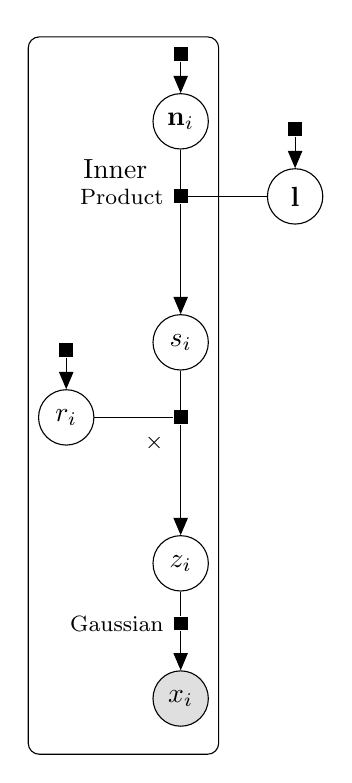
\begin{tikzpicture}

			% \draw[red!20] (-2.4, 2.7) -- (2, 2.7);
			% \draw[red, dotted] (-2.4, 2.7) -- (2, 2.7);
			%
			% \draw[red!20] (-2.4, 5.5) -- (2, 5.5);
			% \draw[red, dotted] (-2.4, 5.5) -- (2, 5.5);

			\node[obs] 											(x)			{$x_i$}; %
			\node[latent, above=of x]                			(z)			{$z_i$}; %

			\factor[above=of z, yshift=10mm] 					{times}		{below left: $\times$} {} {}; %

			\node[latent, above=of times, yshift=-5mm]			(s)			{$s_i$}; %

			\factor[above=of x, yshift=1mm] 					{noise1}	{left:Gaussian} {} {}; %

			\node[latent, left=of times]                		(r)			{$r_i$}; %

			\factor[above=of r] 								{pr}		{} {} {}; %

			\factor[above=of s, yshift=10mm] 					{inner}		{left:Product} {} {}; %

			\node[latent, above=of inner, yshift=-5mm] 			(n)			{$\mathbf{n}_i$}; %
			\node[latent, right=of inner]                		(l)			{$\mathbf{l}$}; %

			\factor[above=of l] 								{pl}		{} {} {}; %

			\factor[above=of n] 								{pn}		{} {} {}; %

			\factoredge {z} 		{noise1} 		{x}; %
			\factoredge {s} 		{times} 		{z}; %
			\factoredge {r} 		{times} 		{}; %
			\factoredge {n} 		{inner} 		{s}; %
			\factoredge {l} 		{inner} 		{}; %
			\factoredge {} 			{pn} 			{n}; %
			\factoredge {} 			{pl} 			{l}; %
			\factoredge {} 			{pr} 			{r}; %

			\plate {} {(pn) (x) (r)} {}; %

			% \fill (r.south) ++ (0, -0.52) circle (3pt) [fill=red] { };
			%
			% \fill (l.south) ++ (0, -0.52) circle (3pt) [fill=red] { };
			%
			% \draw [-stealth, red] (-1.45, 2.85) -- (-1.45, 3.15);
			%
			% \draw [-stealth, red] (1.45, 5.65) -- (1.45, 5.95);

			% \node[yshift=-0.9cm] at (r.south) { $\textcolor{red}{\Delta_i^\mathbf{r}}$ };

			% \node[yshift=-0.9cm] at (l.south) { $\textcolor{red}{\Delta^\mathbf{l}}$ };

			\node[yshift=0.35cm, xshift=-0.83cm] at (inner) { Inner };

		\end{tikzpicture}
		\label{fig:face-model}
	}
  \subfigure[Example face data]{
		\setlength\fboxsep{-0.3mm}
		\setlength\fboxrule{0pt}
		\parbox[b]{3.4cm}{
			\centering
			\small
			\fbox{\includegraphics[width=1.3cm]{figures/sample_N.png}}\\
			Normal $\{\mathbf{n}_i \}$ \vspace{4.5mm} \\
			\fbox{\includegraphics[width=1.3cm]{figures/sample_S.png}} \\
			Shading $\{ s_i \}$ \vspace{4.5mm} \\
			\fbox{\includegraphics[width=1.3cm]{figures/sample_R.png}} \\
			Reflectance $\{ r_i \}$ \vspace{4.5mm} \\
			\fbox{\includegraphics[width=1.3cm]{figures/sample_X.png}} \\
			Observed image $\{ x_i \}$\\
		}
		\label{fig:face-data}
	}
	\mycaption{Sample generative models in computer vision}
  {(a)~Sample renderings from modern graphics engines~\cite{cryengine,lumberyard}.
  Modern graphics provide renderings with stunning level of realism and vision
  problems can be approached as inverting such graphics systems. Images courtesy
  from the official websites of CryEngine~\cite{cryengine} and Lumberyard~\cite{lumberyard}.
  (b)~A layered graphical model (factor graph) for faces (explained in Sec.~\ref{sec:pgm}).
	Here the vision problem
  could be inferring the reflectance map, normal map and light direction from a given
  face image. (c) Sample face data from Yale B face dataset~\cite{Georghiades2001,Lee2005}.}
	\label{fig:sample-gen-models}
\end{figure}

\section{Generative Vision Models}
\label{sec:gen-models}

A conceptually elegant view on computer vision is to consider a generative
model of the physical image formation process. The observed image becomes a
function of unobserved variables of interest (for instance the presence and positions
of objects) and nuisance variables (for instance light sources and shadows).
%
When building such a generative model, we can think of a scene description
$\target$ that produces an image $\obs=G(\target,\theta)$ using a deterministic
rendering engine $G$ with parameters $\params$, or more generally,
results in a distribution over images, $P(\obs|\target,\params)$.
%
Generative models provide a powerful framework for probabilistic reasoning and
are applicable across a wide variety of domains, including computational biology,
natural language processing, and computer vision. For example, in computer vision,
one can use graphical models to express the process by which a face is lit and
rendered into an image, incorporating knowledge of surface normals, lighting and
even the approximate symmetry of human faces. Models that make effective use of this
information will generalize well, and they will require less labelled training data
than their discriminative counterparts (e.g.\ random forests or neural networks) in order
to make accurate predictions.

Given an image observation $\obs$ and a prior over scenes $P(\target)$ we can
then perform \textit{Bayesian inference} to obtain the posterior distribution over the
target variables $P(\target | \obs,\params)$
(also called `posterior inference'):

\begin{equation}
P(\target | \obs,\params) =
\frac{P(\obs|\target,\params)P(\target)}{P(\obs)} =
\frac{P(\obs|\target,\params)P(\target)}{\sum_{\target'} P(\obs|\target',\params)P(\target')}.
\label{eqn:bayes}
\end{equation}

The summation in the denominator runs over all the possible values of $\target$ variable and
would become integral in the case of continuous
variables. $P(\obs|\target,\params)$ is the \emph{likelihood} of the observed data. Inspecting
the above Bayesian formula shows that it is straight forward to compute the numerator
as that involves simply evaluating the generative model. The key difficulty with
Bayesian inference is computing the denominator in Eq.~\ref{eqn:bayes}.
Often, it is not feasible to evaluate the summation
over all the possible target variables even for slightly non-trivial models. This
makes it difficult to obtain closed-form solutions for posterior inference resulting
in the development and use of several approximate inference techniques such
as Markov Chain Monte Carlo (MCMC) sampling and variational inference, which we
will briefly discuss later.

There are different types of generative models with varying model fidelity and
complexity of inference therein. In general, generative models which accurately
model the image formation process (e.g.\ graphics engines) have complex
non-linear functions resulting in a challenging inference task. Building
a good generative model for a given task involves finding a good trade-off
between model fidelity and inference complexity.

Figure~\ref{fig:sample-gen-models} shows some sample generative models in computer vision.
Advances in graphics and physics of light transport resulted in generative models with
high fidelity as is evident in modern computer games and animation movies.
But it is difficult to invert such complex models.
Probabilistic graphical models provide the widely adopted framework
for generative computer vision models. Although graphical models have
less fidelity and only model one or two aspects of the world properties,
they are generally preferred over graphic systems as inference
in them is faster and more reliable. Next, we will discuss these two prominent
generative vision models: \textit{Inverse graphics} and
\textit{Probabilistic graphical models}.

\subsection{Inverse Graphics}
\label{sec:inv-graphics}

Modern graphics engines
(e.g., game engines like CryEngine~\cite{cryengine} and Lumberyard~\cite{lumberyard})
leverage dedicated hardware setups and
provide real-time renderings with stunning level of realism.
Some sample renderings from modern game engines~\cite{cryengine,lumberyard}
are shown in Fig.~\ref{fig:sample-graphics}.
Vision problems can be tackled with posterior
inference (Eq.~\ref{eqn:bayes}) in such accurate computer graphics systems.
This approach for solving vision problems can be understood as
\textit{Inverse Graphics}~\cite{baumgart1974inversegraphics}. The
target variables $\target$ correspond to the input to the graphics system and
the observation variables are the output $\obs=G(\target,\theta)$. The
deterministic graphics system $G$ can be converted into a probabilistic generative
model by defining a prior over the target variables (input to the graphics system) $P(\target)$
and also defining an approximate likelihood function $P(\obs|G(\target,\theta))$
characterizing the model imperfections. If the model imperfections are neglected,
the likelihood can be given using the \emph{delta} function
$P(\obs|\target) = \delta(\obs-G(\target,\theta))$.
An example `inverse graphics' problem, which we tackle in the next chapter,
is depicted in Fig.~\ref{fig:invgraphicsteaser},
where the graphics engine renders a depth image given 3D body mesh
and camera parameters, and a vision problem would be the inverse estimation
of body shape given a depth image.

\begin{figure}[t]
\begin{center}
\centerline{\includegraphics[width=0.7\columnwidth]{figures/invGraphicsDemo.pdf}}
\mycaption{An example `inverse graphics' problem}{A graphics engine renders a 3D
  body mesh and a depth image using an artificial camera. By Inverse
  Graphics we refer to the process of estimating the posterior
  probability over possible bodies given the depth image.}
\label{fig:invgraphicsteaser}
\end{center}
\end{figure}

Modern graphic engines are based on physics principles and thus most of the
rendering parameters $\params$ are set to mimic the real world physics. Learning in graphics
generative models mainly involves learning the prior $P(\target)$
over the target world properties which are input to the graphics system.
Depending on the type of model, several learned priors are proposed in the
literature. An example is the SCAPE model~\cite{anguelov2005scape,hirshberg2012coregistration}
for modeling the prior over human body shape and pose for the example
shown in Fig.~\ref{fig:invgraphicsteaser}.

Since modern rendering engines involve complex non-linear functions, it is
usually not feasible to obtain a closed-form solution for the posterior distribution
(Eq.~\ref{eqn:bayes}). Even several approximate inference techniques like
variational optimization techniques~\cite{koller2009probabilistic} cannot
be easily employed for posterior inference in complex graphics systems.
`Monte Carlo' sampling provides a generic inference technique for
such complex models and can be used even when the internals
of the graphics systems are not known. The aim of sampling methods is to
characterize the posterior distribution with \emph{independent and identically
distributed} samples. There exists many Monte Carlo sampling
strategies such as uniform sampling, rejection sampling,
importance sampling~\cite{hammersley1954poor,rosenbluth1955monte} etc.
Here, we limit our discussion to the widely used Markov Chain Monte Carlo (MCMC)
sampling techniques.

\subsubsection*{MCMC Sampling}
%
MCMC sampling~\cite{metropolis1953} is a
particular instance of sampling methods that generates
a sequence of target variables (samples) by simulating a \textit{reversible}
Markov chain.

\begin{equation}
\target_1 \to \target_2 \to \target_3 \to \dots  \to \target_n
\end{equation}•

This Markov chain of samples approximates the target distribution (posterior
distribution in the case of `inverse graphics'). The Markov property states that
at every sequence step $t$, given the present sample $\target_t$ in the sequence,
the next sample $\target_{t+1}$ is independent of all the previous samples
$P(\target_{t+1}|\target_t,\dots,\target_1) = P(\target_{t+1}|\target_t)$.
%

Let us denote the target distribution with $\pi(\cdot)$. In the inverse
graphics setting, the target distribution is the posterior $\pi(\target)=P(\target | \obs,\params)$.
And, let us denote the transition probability between the two states (samples) in the
Markov chain be $T(\target_{t+1}|\target_{t})$ or $T(\target_t\to\target_{t+1}) \in [0,1]$. One way to ensure that the
Markov chain is \emph{reversible} and converging to the target distribution is to check whether the
following \emph{detailed balance condition} holds for any two states
$\target_t$ and $\targetProp$~\cite{koller2009probabilistic}:

\begin{equation}
\pi(\target_t) T(\target_t \to \targetProp) = \pi(\targetProp) T(\targetProp \to \target_t)
\end{equation}

Note that the above detailed balance condition is satisfied when the transition probability distribution is
close to the target distribution. Since we do not know the target distribution, designing
transition probability distributions that satisfies the detailed balance condition is difficult.
The Metropolis-Hastings (MH) algorithm~\cite{metropolis1953}, instead of devising special transition probabilities,
introduces the \emph{acceptance probability} to each Markov chain transition
$A(\target_t \to \targetProp) \in [0,1]$. The detailed balance condition then becomes:

\begin{equation}
\pi(\target_t) T(\target_t \to \targetProp) A(\target_t\to\targetProp) =
\pi(\targetProp) T(\targetProp \to \target_t) A(\targetProp\to\target_t)
\end{equation}

It can be verified~\cite{koller2009probabilistic} that the following acceptance
probability satisfies the above detailed balance condition:

\begin{equation}
A(\target_t\to\targetProp) = \min\left(1,\frac{\pi(\targetProp)
T(\targetProp \to \target_t)}{\pi(\target_t) T(\target_t \to \targetProp)} \right)
\end{equation}

With the use of the above acceptance rule, instead of designing task-specific
transition probability distributions,
any transition probability distribution $T$ with non-zero probability over
the range of all target variables can be used for MH sampling. $T$ is also
called `proposal distribution' since it is used to propose the next sample in the
Markov chain, which is then either accepted or rejected based on the acceptance probability.
Below, we summarize the Metropolis-Hastings (MH) MCMC algorithm.

\paragraph{Metropolis-Hastings (MH) MCMC:}
Sampling from $\pi(\cdot)$ consists of repeating the
following two steps~\cite{liu2001montecarlo}:

\begin{enumerate}
\item Propose a transition using a \textit{proposal distribution $T$}
  and the current state $\target_t$
\begin{equation*}
\targetProp \sim T(\cdot|\target_t)
\end{equation*}
\item Accept or reject the transition based on Metropolis Hastings (MH) acceptance rule:
\begin{equation*}
\target_{t+1} = \left\{
  \begin{array}{cl}
      \targetProp,  & \textrm{rand}(0,1) < \min\left(1,\frac{\pi(\targetProp)
T(\targetProp \to \target_t)}{\pi(\target_t) T(\target_t \to \targetProp)} \right), \\
     \target_t, & \textrm{otherwise.}
  \end{array}
\right.
\end{equation*}
\end{enumerate}

% Kernel T
Different MCMC techniques mainly differ in the type of the
proposal distribution $T$. Note that we do not need to compute the target (posterior)
probabilities, but only the \textit{ratio} of
posterior probabilities $\frac{\pi(\targetProp)}{\pi(\target_t)}$.
This makes MCMC sampling suitable for the inverse graphics setting
where it is not feasible to get a closed-form solution for the normalization
constant in the posterior distribution (denominator in Eq.~\ref{eqn:bayes}).

The key aspect of the MH sampling is the number of steps it requires until
it converges to the target distribution. If the proposal distribution is very
different from the target distribution, the samples tend to be frequently rejected
resulting in a long wait for convergence. In practice, it is difficult to
measure the convergence of any sampler since we do not know the target
distribution. In Chapter~\ref{chap:infsampler}, we discuss several diagnostic
measures that indicate the convergence of MCMC sampling. In the case of
`inverse graphics', each forward rendering step takes a considerable amount of time and
we would like the sampler to accept as many samples as possible. A key for improving
the MH sampling efficiency is to design the proposal distributions that match
the target posterior distribution. In Chapter~\ref{chap:infsampler}, we devise
such technique by leveraging discriminative learning techniques for learning
the proposal distribution. Refer to~\cite{liu2001montecarlo,koller2009probabilistic}
for more details on MCMC sampling. In Chapter~\ref{chap:infsampler}, we study
the behavior of MCMC sampling and its variants for inverting graphics
engines and propose techniques for improving the sampling efficiency.

\subsection{Probabilistic Graphical Models}
\label{sec:pgm}

Probabilistic graphical models (PGM) provide a rigorous mathematical framework,
based on probability and graph theory, for modeling the relationship between
the world and image properties.
PGMs have been popular not only in computer vision but also in
related fields such as natural language processing,
speech processing, etc. Several model representations, learning and inference
schemes haven been developed in the PGM literature and even a concise description
of them would be an inundating task and is outside the scope of this thesis. Refer
to~\cite{koller2009probabilistic} for a comprehensive overview of PGMs.
PGMs generally represent input-output relationships with
factorized functions and are typically confined to a restricted domain so that
efficient inference techniques can be applied.

PGMs are popular models of choice when the joint distribution of all the target
and observation variables can be factorized into independent distributions
each involving a subset of variables. This factorization of the joint distribution
is represented with the structure of the graph, where each node represents a subset
of variables and edges between the nodes represent the joint or conditional
distributions between the corresponding node variables.

\begin{figure}[t]
	\centering
		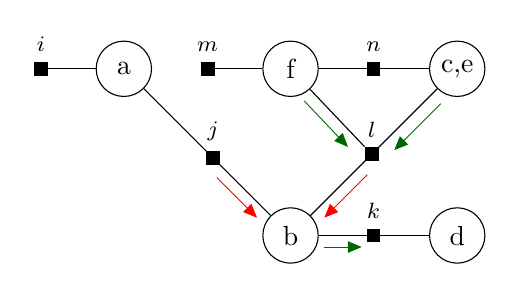
\begin{tikzpicture}

			\node[latent] (var_a) {a};
			\node[latent, right=of var_a, xshift=4mm] (var_f) {f};
			\node[latent, right=of var_f, xshift=4mm] (var_ce) {c,e};
			\node[latent, below=of var_f, yshift=-4mm] (var_b) {b};
			\node[latent, below=of var_ce, yshift=-4mm] (var_d) {d};

			\factor[left=of var_a, xshift=-2mm] {factor_a} {$i$} {} {};
			\factor[left=of var_f, xshift=-2mm] {factor_f} {$m$} {} {};
			\factor[below right=of var_a, xshift=5mm, yshift=-5mm] {factor_ab} {$j$} {} {};
			\factor[above right=of var_b, xshift=4mm, yshift=4mm] {factor_fceb} {$l$} {} {};
			\factor[right =of var_b, xshift=2mm] {factor_bd} {$k$} {} {};
			\factor[right =of var_f, xshift=2mm] {factor_fce} {$n$} {} {};

			\edge[-] {factor_a} {var_a};
			\edge[-] {factor_f} {var_f};
			\edge[-] {var_a} {var_b};
			\edge[-] {var_b} {var_ce};
			\edge[-] {var_f} {factor_fceb};
			\edge[-] {var_b} {var_d};
			\edge[-] {var_f} {var_ce};

			\edge[->, transform canvas={xshift=8.4mm,yshift=-2.4mm,scale=0.8},black!60!green] {var_ce} {factor_fceb};
			\edge[->, transform canvas={xshift=4mm,yshift=-2mm,scale=0.8},black!60!green] {var_f} {factor_fceb};
			\edge[->, transform canvas={xshift=6.5mm,yshift=-4mm,scale=0.8},red] {factor_fceb} {var_b};
			\edge[->, transform canvas={xshift=0.56cm,yshift=-5.7mm,scale=0.8},black!60!green] {var_b} {factor_bd};
			\edge[->, transform canvas={xshift=0.2cm,yshift=-4mm,scale=0.8},red] {factor_ab} {var_b};

		\end{tikzpicture}
		\label{fig:example-graph}
	\mycaption{An example factor graph}{Variable nodes (circles) and factor nodes (squares) representing
	the factorized function
	$P(a,b,c,d,e,f)=\psi_i(a)\psi_j(a,b)\psi_k(b,d)\psi_l(b,c,e,f)\psi_m(f)\psi_n(c,e,f)$. Also shown are sample
	variable-to-factor messages (green arrows) and, factor-to-variable messages (red arrows).}
\end{figure}

\subsubsection{Factor Graph Representation}

Factor graphs provide a useful visualization and mathematical formalization for representing probabilistic
graphical models. Factor graphs are \emph{bipartite} graphs where nodes in the graph
are divided into two types: `variable' nodes represented as circles and `factor' nodes
represented as squares. Variable nodes represent the random variables in the graphical model and
factor nodes represent the statistical relationship between the variable nodes that they are connected to.
Every edge in the factor graph connects a variable node to factor node. That is,
there are no \emph{direct} edges among the variable nodes or factor nodes. An example
factor graph is shown in Fig.~\ref{fig:example-graph}, where we represent variable nodes
as $a,b,c,\cdots$ and factor nodes as $i,j,k,\cdots$. The factor function associated with
a factor node $a$ is represented as $f_a$ and the states of variables associated with
a variable node $i$ is represented as $i$.
The joint function in Fig.~\ref{fig:example-graph},
$P(a,b,c,d,e)$ is factorized into five independent factors
$\psi_i(a)\psi_j(a,b)\psi_k(b,d)\psi_l(b,c,e,f)\psi_m(f)f_n(c,e,f)$.
Each factor in the graph represent a function and the product of all factor functions makes
up the joint function. In the context of probabilistic generative models, these
functions are probability distributions. The edges in the factor can be either directed
or un-directed representing the joint and conditional distributions respectively.
In the case of discrete variables, the factor functions are probability tables
assigning the probabilities for all the states of the factor variables. And, in the
case of continuous variables, the factor functions are probability density functions.
Another example of factor graph, representing a generative model of faces, is
shown in Fig.~\ref{fig:face-model}. We will discuss more about this face model later
in this section.

Graphical representations like factor graphs have several advantages. They provide
an intuitive way of representing the statistical dependencies between the variables.
Given the factor graph, it is easy to visualize \emph{conditional independence}
between variables.
For a factor graph with undirected edges, variables $s$ and $t$ are independent
given a set of variables $\nu$ ($s \ci t | \nu$)
if every path between $s$ and $t$ have some node $v\in\nu$.
For instance, in the factor graph shown in Fig.~\ref{fig:example-graph},
variable $d$ is independent of $a,c,e$ and $f$ given $b$ is observed: $d \ci a,c,e,f | b$.
Perhaps the most important advantage of graphical representations like factor graphs
is that we can perform Bayesian inference by using the graph structure. For example, the widely used
\emph{message-passing} inference is performed by passing messages between factor and variable nodes.

\subsubsection{Message Passing} Message Passing (MP) inference forms a general class
of algorithms that are used to estimate the factor graph distributions,
i.e. maximizing or minimizing the joint distribution (P(a,b,c,d,e,f) in Fig.~\ref{fig:example-graph}).
MP inference proceeds by passing messages (distributions or density functions)
between variable and factor nodes. Here, we describe the message passing in the
famous `Sum-Product' belief-propagation (BP) algorithm.
Messages are probability distributions that represent the beliefs
over the variables to/from which the messages are being sent.
MP inference in factor graphs has two types of messages: Messages
from variable to factor nodes $\mu_{a\rightarrow i}$ (green arrows in Fig.~\ref{fig:example-graph})
and messages from factor to variable nodes $\mu_{i\rightarrow a}$
(red arrows in Fig.~\ref{fig:example-graph}).
In the case of Sum-Product BP, these messages are defined as follows.

\textit{Variable-to-Factor Message:} A message from variable to factor node
is the product of all the messages that the variable node receives from its
neighboring factor nodes except the recipient factor node.
In Fig.~\ref{fig:example-graph}, the message $\mu_{b \rightarrow m}$
from variable $b$ to factor $m$ is the product of the messages that $b$ receives,
i.e. $\mu_{k \rightarrow b} \mu_{l \rightarrow b}$. In general, a message from
a variable node $g$ to factor node $r$ is defined as:

\begin{equation}
\mu_{g \rightarrow r}(x_g) = \prod_{\hat{r}\in N(g)\setminus \{r\}} \mu_{\hat{r} \rightarrow g}(x_g),
\end{equation}

where $N(g)$ is the set of neighboring nodes to $g$ and $x_g$ represent the states
of $g$.

\textit{Factor-to-Variable Message:} A message from factor to variable node
is first computed as the product of factor function with all the incoming messages
from variables except the target variable. The resulting product is then marginalized
over all the variables except the one associated with the target node variables.
For example, in Fig.~\ref{fig:example-graph}, the message from $l$ to $b$ is computed
by marginalizing the product $\psi_l(b,c,e,f)\mu_{c,e\rightarrow l}\mu_{f\rightarrow l}$
over non-target variables $c,e,f$. In general, a message from factor node $r$
to variable node $g$ is defined as:

\begin{equation}
\mu _{r\to g}(x_g)=\sum _{x':V_{r}\setminus g} \psi_{r}(x')\prod_{\hat{g}\in
N(r)\setminus \{g\}}\mu _{\hat{g}\to r}(x_{\hat{g}}),
\end{equation}

where $N(r)$ represents the neighboring nodes of $r$ and $V_r$ represent all the variables
attached to $r$. The summation in the above equation becomes an integral when
dealing with continuous variables.

In a typical message passing inference run, the above messages are repeatedly computed
and sent between factor and variable nodes. Depending on the structure of the factor graph,
different message priorities are used. Upon convergence or passing messages for a
pre-defined number of iterations, the marginal distribution at each variable node is
computed as the product of all its incoming messages from the neighboring factor nodes:

\begin{equation}
P(x_g) = \prod_{\hat{r}\in N(g)} \mu_{\hat{r} \rightarrow g}(x_g).
\end{equation}

Messages represent a probability of each possible state of a variable.
In the case of discrete variables with small number of states, it is easy to represent
messages as probability distribution tables. However, in the case of continuous variables,
the messages must be full functions of the variables. Some approximations are typically
required to represent messages with continuous distributions.
Different message passing algorithms differ in the way the messages are approximated.
Some MP algorithms assume Gaussian form for the messages with either restricting
the type of factor functions~\cite{weiss2001correctness} that always result in Gaussian messages or
projecting the computed messages into Gaussian form~\cite{Minka2001}.
Some other MP algorithms use mixture of Gaussians~\cite{sudderth2010nonparametric} or set of
particles/samples~\cite{ihler2009particle} for representing messages.


\subsubsection{Variational Inference}
Except for small graphical models, exact Bayesian inference (say, with
the above mentioned Sum-Product BP) in PGMs is
usually not possible. This is especially true for computer vision models which
typically involve several hundreds or thousands of variables.
Variational Bayesian inference is one of the widely used technique for performing
inference in PGMs. These methods try to find an
approximation $Q(\target)$ to the true posterior distribution $P(\target|\obs)$
via optimization techniques.
This approximate distribution is usually taken from a known simpler family
of distributions (such as exponential family) and the optimization is
performed over the space of that family of distributions. For example, for the
above joint distribution function $P(a,b,c,d,e,f)$,
an approximation could be a factorized distribution
$Q = Q_1(a) Q_2(b) Q_3(c) Q_4(d) Q_5(e) Q_6(f)$, each from an exponential family of distributions.
The most commonly used optimization function is minimizing the
Kullback-Leibler (KL) divergence of $P$ from $Q$ in order to find a close approximation
to $P$:

\begin{equation}
D_{KL}(Q||P) = \underbrace{\sum_z Q(\target) \frac{Q(\target)}{P(\target,\obs)}}_{-\mathcal{L}(Q)} +
\log P(\obs)
\label{eqn:kl}
\vspace{-0.2cm}
\end{equation}

Minimizing the above KL-divergence translates to maximizing the variational
lower bound $\mathcal{L}(Q)$ as $P(\obs)$ is constant.
$\mathcal{L}(Q)$ is also called \textit{energy functional} or
\textit{variational free energy} as it can be written as the sum of energy
$\mathbb{E}_Q[\log P(\target,\obs)]$ and the entropy of $Q$. $Q$ is chosen
in such a way that $\mathcal{L}(Q)$ becomes tractable and maximizable.

In general, the energy functional is maximized by passing messages between different
variable nodes in the factor graph (e.g. factor graphs in
Figs.~\ref{fig:example-graph},~\ref{fig:face-model}).
Following~\cite{koller2009probabilistic}, depending on the type of approximations
to $Q$ and the energy functional, methods for maximizing $\mathcal{L}(Q)$ can
be categorized into three types. The first category of methods optimizes approximate
versions of the energy functions by passing messages in the simplified versions of the
given factor graph. This includes the
\textit{loopy belief propagation}~\cite{frey1998revolution,weiss2000correctness} algorithm.
The second category of methods try to maximize the exact energy functional but
uses approximate message propagation steps, for example approximating complex
messages with distributions from the exponential family. This is equivalent to using
relaxed consistency constraints on $Q$. These class of methods are also known as
\textit{expectation propagation} (EP)~\cite{Minka2001} algorithms.
The third commonly used category of methods maximize the exact energy functional
but restrict $Q$ to simple factorized distributions, which is called \textit{mean-field}
approximation. One of the most commonly used message passing technique for
optimizing the energy functional is \textit{variational message passing} (VMP)~\cite{Winn2005}.
In Chapter~\ref{chap:cmp}, we show how EP and VMP fail to converge for inference
in model shown in Fig.~\ref{fig:face-model} and propose a remedy for that.

Several other inference techniques such as MCMC sampling can be used for inference
in PGMs. Refer to~\cite{fox2012tutorial} for a tutorial on variational Bayesian
inference and to~\cite{koller2009probabilistic,wainwright2008graphical}
for a comprehensive review of various inference techniques in PGMs.

\subsubsection{Two Example Models}
\label{sec:example_modesl_crf}
Here, we give a brief overview of two popular types of
PGMs in vision which are later used in this thesis:
Layered graphical models and fully connected CRFs.

\paragraph{Layered Graphical Models:} Several vision models are hierarchical
in nature and can be naturally expressed
with layered graphical models. Figure~\ref{fig:face-model} shows an example
layered \textit{factor graph} model for faces. Here, a vision task could be:
Given an observation of pixels $\mathbf{x} = \{x_i\}$,
we wish to infer the reflectance value $r_i$ and normal vector $\mathbf{n_i}$
for each pixel $i$ (see Fig.~\ref{fig:face-data}).
The model shown in Fig.~\ref{fig:face-model} represents the following approximate image
formation process: $x_i = (\mathbf{n_i} \cdot \mathbf{l}) \times r_i + \epsilon$,
thereby assuming Lambertian reflection and an infinitely distant directional
light source with variable intensity. Each factor in the graph is a
conditional probability distribution providing the factorization for the
joint distribution:

\begin{equation}
P(\obs, \mathbf{z}, \mathbf{r}, \mathbf{s}, \mathbf{n}, \mathbf{l})
= P(\mathbf{n}) P(\mathbf{l}) P(\mathbf{r}) \prod_i P(x_i) P(x_i | z_i)
P(z_i | r_i, s_i) P(s_i | \mathbf{n}_i, \mathbf{l}),
\end{equation}

where $s_i$ and $z_i$ represent the intermediate shading and non-noisy
image observation variables. We omitted the model parameters $\params$
in the above equation for the sake of simplicity.
A vision task could to estimate the posterior distribution
$P(\mathbf{r}, \mathbf{s}, \mathbf{n}, \mathbf{l} | \obs)$.
Note that this generative model is only a crude
approximation of the true image formation process
(e.g. each pixel is modeled independently and it does not account for
shadows or specularities). Such approximations are customary to PGMs as
several PGM inference techniques cannot be applied for models with complex
non-linear factors. Note that even for a relatively small image of
size $96 \times 84$, the face model contains over 48,000 latent variables
and 56,000 factors, and as we will show in Chapter~\ref{chap:cmp},
standard message passing routinely fails to converge to
accurate solutions.

\definecolor{city_1}{RGB}{128, 64, 128}
\definecolor{city_2}{RGB}{244, 35, 232}
\definecolor{city_3}{RGB}{70, 70, 70}
\definecolor{city_4}{RGB}{102, 102, 156}
\definecolor{city_5}{RGB}{190, 153, 153}
\definecolor{city_6}{RGB}{153, 153, 153}
\definecolor{city_7}{RGB}{250, 170, 30}
\definecolor{city_8}{RGB}{220, 220, 0}
\definecolor{city_9}{RGB}{107, 142, 35}
\definecolor{city_10}{RGB}{152, 251, 152}
\definecolor{city_11}{RGB}{70, 130, 180}
\definecolor{city_12}{RGB}{220, 20, 60}
\definecolor{city_13}{RGB}{255, 0, 0}
\definecolor{city_14}{RGB}{0, 0, 142}
\definecolor{city_15}{RGB}{0, 0, 70}
\definecolor{city_16}{RGB}{0, 60, 100}
\definecolor{city_17}{RGB}{0, 80, 100}
\definecolor{city_18}{RGB}{0, 0, 230}
\definecolor{city_19}{RGB}{119, 11, 32}
\begin{figure}[t]
  \scriptsize % scriptsize
  \centering
 \fcolorbox{white}{city_1}{\rule{0pt}{1pt}\rule{1pt}{0pt}} Road~~
 \fcolorbox{white}{city_2}{\rule{0pt}{1pt}\rule{1pt}{0pt}} Sidewalk~~
 \fcolorbox{white}{city_3}{\rule{0pt}{1pt}\rule{1pt}{0pt}} Building~~
 \fcolorbox{white}{city_4}{\rule{0pt}{1pt}\rule{1pt}{0pt}} Wall~~
 \fcolorbox{white}{city_5}{\rule{0pt}{1pt}\rule{1pt}{0pt}} Fence~~
 \fcolorbox{white}{city_6}{\rule{0pt}{1pt}\rule{1pt}{0pt}} Pole~~
 \fcolorbox{white}{city_7}{\rule{0pt}{1pt}\rule{1pt}{0pt}} Traffic Light~~
 \fcolorbox{white}{city_8}{\rule{0pt}{1pt}\rule{1pt}{0pt}} Traffic Sign~~\\
 \fcolorbox{white}{city_9}{\rule{0pt}{1pt}\rule{1pt}{0pt}} Vegetation~~
 \fcolorbox{white}{city_10}{\rule{0pt}{1pt}\rule{1pt}{0pt}} Terrain~~
 \fcolorbox{white}{city_11}{\rule{0pt}{1pt}\rule{1pt}{0pt}} Sky~~
 \fcolorbox{white}{city_12}{\rule{0pt}{1pt}\rule{1pt}{0pt}} Person~~
 \fcolorbox{white}{city_13}{\rule{0pt}{1pt}\rule{1pt}{0pt}} Rider~~
 \fcolorbox{white}{city_14}{\rule{0pt}{1pt}\rule{1pt}{0pt}} Car~~
 \fcolorbox{white}{city_15}{\rule{0pt}{1pt}\rule{1pt}{0pt}} Truck~~\\
 \fcolorbox{white}{city_16}{\rule{0pt}{1pt}\rule{1pt}{0pt}} Bus~~
 \fcolorbox{white}{city_17}{\rule{0pt}{1pt}\rule{1pt}{0pt}} Train~~
 \fcolorbox{white}{city_18}{\rule{0pt}{1pt}\rule{1pt}{0pt}} Motorcycle~~
 \fcolorbox{white}{city_19}{\rule{0pt}{1pt}\rule{1pt}{0pt}} Bicycle~~\\
  \subfigure[Sample Image]{%
    \includegraphics[width=.45\columnwidth]{figures/frankfurt00000_008206_given.png}
  }\hspace{4.5mm}
  \subfigure[Ground Truth Semantics]{%
    \includegraphics[width=.45\columnwidth]{figures/frankfurt00000_008206_gt.png}
  }
  \mycaption{Illustration of semantic segmentation task}{A sample image from
  Cityscapes street scene dataset~\cite{Cordts2015Cvprw} and the corresponding
  ground truth semantic labels.}
\label{fig:example-seg}
\end{figure}


\paragraph{Fully Connected CRFs:} Fully connected conditional random fields,
also known as DenseCRFs, are CRF models where every variable in the image is connected to
every other variable via pairwise edge potentials. For illustration purposes,
let us consider the task of semantic segmentation which is labelling each pixel
in a given image with a semantic class. See Fig.~\ref{fig:example-seg} for an
illustration. For the segmentation problem, DenseCRFs
are generally used to encode the prior knowledge about the problem:
`Pixels that are spatially and photometrically similar are more likely to have the same label'.

For an image $\obs$ with $n$ pixels, the semantic segmentation task is to produce a
labelling $\target$ with discrete values
$\{y_1,\dots,y_n\}$ in the label space $y_i\in\{1,\ldots,\mathcal{L}\}$. The DenseCRF model has
unary potentials $\psi_u(y)\in\mathbb{R}$, e.g., these can be the output of CNNs.
The pairwise potentials, as introduced in~\cite{krahenbuhl2012efficient},
are of the form $\psi^{ij}_p(y_i,y_j) = \mu(y_i,y_j) k(\f_i,\f_j)$
where $\mu$ is a label compatibility matrix, $k$ is a Gaussian kernel
$k(\f_i,\f_j)=\exp(-(\f_i-\f_j)^{\top}\Sigma^{-1}(\f_i-\f_j))$ and
the vectors $\f_i$ are feature vectors at each point. Commonly used features are
position and color values at the pixels (e.g., $\f=(x,y,r,g,b)^\top$).
In the DenseCRF model, the energy functional for an image $\obs$ thus reads:

\begin{equation}
P(\target|\obs)\propto\exp(-\sum_i\psi_u(y_i)-\sum_{i>j}\psi^{ij}_p(y_i,y_j)).
\end{equation}

Because of the dense connectivity, exact MAP or marginal inference is intractable. The main result
of~\cite{krahenbuhl2012efficient} is to derive the mean-field approximation for this model and to relate it
to bilateral filtering which enables tractable approximate inference.
As described above, mean-field approximation is a type of variational inference
where the approximate distribution $Q$ is considered to be fully-factorized
across pixels:
$Q=\prod_{i \in n} Q_i(x_i)$. Variational inference then solves for $Q$ by minimizing
the KL divergence of $P$ from $Q$(see Eq.~\ref{eqn:kl}).The work of~\cite{krahenbuhl2012efficient}
showed that the inference can be performed with efficient bilateral filtering
~\cite{aurich1995non, smith97ijcv, tomasi1998bilateral, adams2010fast} operations.
Specifially, mean-field inference results in a fixed point equation which
can be solved iteratively $t=0,1,\ldots$ to update the marginal distributions $Q_i$:

\begin{equation}
Q^{t+1}_i(x_i) = \frac{1}{Z_i} \exp(-\psi_u(x_i) - \sum_{l \in \mathcal{L}}\underbrace{\sum_{j \ne i}
\psi^{ij}_p(x_i,l) Q^{t}_j(l)}_\text{bilateral filtering}),
\label{eq:mfupdate}
\end{equation}

where $Z_i$ denotes a normalization constant and can be easily computed as $Q_i$ is
a single dimensional distribution. Although we used semantic segmentation task
for illustration purposes, DenseCRFs are shown to be useful for tackling
other tasks such as material segmentation~\cite{bell2015minc}, optical flow
estimation~\cite{sun2013fully} and intrinsic image decomposition~\cite{bell2014intrinsic}.

One of the fundamental limitations of the existing use of DenseCRFs is the
confinement of pairwise potentials $\psi^{ij}_p(y_i,y_j)$ to be Gaussian as
bilateral filtering is traditionally implemented with a Gaussian kernel. In Chapter~\ref{chap:bnn},
we show how we can learn a more general form of bilateral filters and
apply that technique for learning pairwise edge potentials in DenseCRF.

\subsection{Advantages and Limitations}
\label{sec:gen-adv-limits}

This generative modeling view is appealing as it is relatively easy to incorporate our knowledge
of physics and light transport into models and was advocated since the late
1970~\cite{horn1977imageintensities,
grenander1976patterntheory,zhu1997learning,mumford2010patterntheory,
mansinghka2013approximate,yuille2006vision}.
For example, the knowledge of how light reflects on objects with different
material properties or the knowledge of how roads and buildings are structured
are relatively easy to incorporate into generative models.
Due to incorporation of strong prior knowledge into the systems, generative
models usually work better when there is little or no data available for a
particular problem.
Since a single generative model can model different world and image
characteristics, it can be used for many different applications.
In addition, it is easier to diagnose the flaws in generative model as most
of the model is manually designed.

% Depressive perspective: 30 years of non-working models
Despite its intuitive appeal and advantages,
in practice, generative models are used only for a few vision problems.
The few successes of the idea have been in limited settings.
In the successful examples, either
the generative model was restricted to few high-level latent
variables, e.g.,~\cite{oliver2000humaninteractions},
or restricted to a set of image transformations in a fixed reference
frame, e.g.,~\cite{black2000imageappearance},
or it modeled only a limited aspect such as
object shape masks~\cite{eslami2012shapeboltzmann},
or the generative model was merely used to generate
training data for a discriminative model~\cite{shotton2011kinect,gaidon2016virtual,
ros2016synthia,richter2016playing,shafaei2016play}.
%
With all its intuitive appeal, its beauty and simplicity, it is fair to say
that the track record of generative models in computer vision is poor.
%
As a result, the field of computer vision is now dominated by
efficient but data-hungry discriminative models,
the use of empirical risk minimization for learning,
and energy minimization on heuristic objective functions for inference.

% What is the challenge in this picture?
Why did generative models not succeed? There are two key problems that
need to be addressed, the design of an accurate generative model, and
the inference therein.
The first key problem which is the design of accurate generative model is partly
addressed by recent advances in graphics. Although modern graphics provide
rendering with stunning level of realism, priors of world parameters are difficult
to characterize. This results in complex priors together with more complex
forward models for accurate generative models which in turn results in
difficult inference.

This brings us to the second key problem in the generative world view which is
the difficulty of posterior inference at test time.
%
This difficulty stems from a number of reasons:
\emph{first}, the target variable $\target$ is typically high-dimensional and so is
the posterior.
%
\emph{Second}, given $\target$, the image formation process realizes complex and
\emph{dynamic} dependency structures, for example when objects occlude or
self-occlude each other. These intrinsic ambiguities result in multi-modal
posterior distributions.
%
\emph{Third}, while most renderers are real-time, each simulation of the
forward process is expensive and prevents exhaustive enumeration. Overall,
the limitations of generative approaches out-weigh their advantages making
them not succeed in building practical computer vision systems.

Despite these limitations, we still believe in the usefulness of generative
models in computer vision, but argue that we need to leverage existing discriminative
or even heuristic computer vision methods for alleviating some of the difficulties in the
posterior inference. Inference techniques proposed in this thesis are steps
in this direction.

\section{Discriminative Vision Models}

With the advances in internet and image capturing technology, there is an explosive
growth of visual data during the last few years. Moreover, presence of crowd-sourcing
platforms like `Amazon Mechanical Turk'~\cite{mturk} make it easier to annotate large
amounts of data by millions of people. Discriminative models directly model the
contingency of world properties on the observed data $P(\target|\obs)$.
Unlike generative models, discriminative
models are task-specific and learning takes the central role in defining the model.
Discriminative models comprise of functions directly approximating
the posterior distribution $P(\target|\obs, \params)$, where $\params$ denote
the parameters of the model. Supervised learning with annotated training data
is usually employed to fit the model parameters to the given task.
Since discriminative models directly characterize
the posterior distribution, inference is reduced to simple evaluation of
the model.

Due to the availability of large amounts of training data and the computing power
that can handle rich high-capacity models, discriminative models have been very
successful in many vision problems. In addition, inference is fast
since this involves a simple evaluation of the model. This makes discriminative
models particularly attractive for many practical applications. Many
mathematical functions that are rich enough to capture the relationship between
the observation and target variables can be used as discriminative models.
Hence, many types of discriminative models have been used in the computer vision
literature.

Discriminative models are traditionally partitioned into two modules:
\textit{feature extraction} and \textit{prediction} modules.
Before the advent of modern convolutional neural networks (CNNs),
these two components are studied separately in the literature.
We briefly discuss these two components in the discriminative models.

\paragraph{Feature Extraction:}
Depending on the type of vision task, features are extracted either at all
pixels (points) in the observed data or only at some key points. For example,
registering two images taken from different view-points requires finding
corresponding points (key points) in each image and then matching.
For such tasks, an additional step of key point detection is required before
feature computation. For image classification, a single feature vector
is extracted for the entire image.

An ideal feature representation should be compact, efficient to compute
and invariant to specific transformations. As an example,
for semantic segmentation, features should be invariant to intra-class
variations such as illumination, scale, rotation, object articulations, etc.,
while being sensitive to changes across different semantic categories.
Several feature extraction schemes have
been proposed in the vision literature, most of them are hand crafted.
Some popular choices include SIFT~\cite{lowe1999object}, HoG~\cite{bay2006surf},
SURF~\cite{dalal2005histograms}, DAISY~\cite{tola2008fast}, etc.
Models for feature extraction and prediction are plentiful and discussing
all of them is outside the scope of this thesis.
With the recent advances in CNNs, feature extraction is coupled with
prediction which are learned together end-to-end.

\paragraph{Prediction:}
Once the image features are extracted, the task is to estimate the
posterior distribution $P(\target|\f(\obs))$, where $\f(\obs)$ denotes the features.
A common strategy is to learn a rich parametric or non-parametric model with
supervised learning techniques. This makes the availability of training data
crucial for discriminative approaches. Several learning based prediction
models have become popular in tackling vision tasks including support vector
machines (SVM)~\cite{cortes1995support},
boosting~\cite{schapire1990strength, freund1995desicion},
random forests~\cite{breiman2001random,ho1995random},
deep convolutional neural networks~\cite{lecun1998gradient},
etc. Refer to~\cite{friedman2001elements}
for a review of different prediction techniques.
Next, we briefly review random forests and CNN models as we either make use of
or propose extensions to these models in this thesis.

\subsection{Random Forests}
\label{sec:forests}

Random forests~\cite{breiman2001random,ho1995random}
are an ensemble of $K$ randomly trained prediction (classification or regression)
trees, where each tree $T(\target|\f(\obs),\params^k)$ represents a non-linear
function approximating the posterior $P(\target|\f(\obs))$.
The trees are typically binary trees and can be viewed as performing a
discriminative hierarchical clustering of the feature space.
And a simple model fit (e.g.,\ linear model) is used in each cluster.

Trees are grown incrementally from the root node to the leaves and
each node represents a partition of the feature space. These partitions can be any linear
or non-linear functions, but the simple axis-aligned partitions are the most used ones
due to their simplicity and efficiency. For simplicity, let us assume the partition functions
are axis-aligned. At each node, a feature $\kappa$ and
its split value $\tau$ are chosen to split the feature space,
so as to minimize an energy function $E$. Let us
consider training the $j^{th}$ node in a $k^{th}$ tree. Let all the data points falling
in that node be $\mathcal{S}_j$ (due to splitting of its ancestor nodes)
and $\mathcal{T}_j$ denotes the discrete set of
\textit{randomly} selected feature axes $\{(\kappa,\tau)_i\}$
(feature indices and their corresponding values)
for the node $j$. Training the $j^{th}$ node corresponds to choosing the optimal
split $\theta^k_j \in \mathcal{T}_j$ among the randomly chosen splits that
minimizes an energy function $E$:

\begin{equation}
\theta^k_j = \argmin_{\gamma \in \mathcal{T}_j} E(\mathcal{S}_j,\gamma)
\end{equation}

Depending on the type of task and data, different energy functions $E$ are
used. Each split $\gamma$ partitions the training data $\mathcal{S}_j$ in
the node $j$ into two parts $\mathcal{S}^L_j$ and $\mathcal{S}^R_j$ which are
assigned to left and right child nodes respectively.
A common energy function measures how well a regression/classification model
fit the data in each of the left and right child nodes created by a split $\gamma$:

\begin{equation}
E(\mathcal{S}_j,\gamma) = - (M(\mathcal{S}^L_j, \beta) + M(\mathcal{S}^R_j, \beta)).
\label{eqn:forest_energy}
\end{equation}

Where $M(\mathcal{S}_j,\beta)$ denotes the model likelihood i.e., how well the model with parameters
$\beta$ can explain the data $\mathcal{S}_j$.
For example, in the case of regression tasks, $M$ can be a linear regression fit
and in the case of classification
(like in semantic segmentation), $M$ can be the classification accuracy.
Like this, the trees are recursively grown by splitting the leaf nodes into left and right
child nodes. The set of all node splits $\theta^k=\{\theta^k_j\}_{j=1,\cdots,J}$ represents
the parameters of the $k^{th}$ tree.
Once a tree is trained, a simple prediction
model is fitted to the data in the leaf nodes. A deep tree might overfit the data
and a shallow tree would under-fit the data and miss important structure. Restricting
the tree size corresponds to regularizing the model and size should be adaptively
chosen based on the training data. Some training stopping criteria include setting the
maximum depth of the trees; minimum number of data points in each node;
a threshold for energy function $E$, etc.

Random forests are distinguished from other tree-based
supervised learning techniques such as boosted decision trees, by the way different
trees are trained in a forest. Each tree in a random forest is trained independently
and randomness is added either in terms of choosing a random subset of training data for each
tree (called \textit{bagging}~\cite{breiman1996bagging}) and/or randomly
choosing the split candidates (feature indices and their values) at each node.
Typically, the estimates across the trees $T(\target|\f(\obs),\params^k)$
are averaged to get the final model $P(\target|\f(\obs))$:

\begin{equation}
P(\target|\f(\obs)) = \frac{1}{K}\sum_{k} T(\target|\f(\obs),\params^k).
\end{equation}

Due to the randomness, different trees are identically distributed
resulting in a low-variance estimate when the final estimate is taken as the average
across the trees.
Random forests are highly flexible and several different types of models are
conceivable with using a combination of different splitting criteria.
Due to their simplicity and flexibility, random forests have become a popular
choice for supervised learning in vision.
Random forests are easy to implement and train. Also, they can be easily adapted
to a wide range of classification and regression tasks with relatively simple
changes to the model. Moreover, they are non-parametric in
nature with the ability to consume large amounts of training data.
Random forests are successfully applied for vision tasks such as
human pose estimation~\cite{shotton2011kinect}, semantic segmentation~\cite{shotton2008semantic}, etc.
In the case of semantic segmentation, a popular model is to extract TextonBoost
features~\cite{shotton2006textonboost}
at each pixel and then train a random forest classifier to predict the class
label at each pixel.
One of the crucial advantages of random forests with respect
to neural networks is that the loss function $E$ need not be differentiable.
In Chapter~\ref{chap:infsampler}, we use random forest models
to improve inference in inverse graphics via our informed
sampler approach. In Chapter~\ref{chap:cmp}, we use random forests
for predicting messages resulting in improved variational inference in
layered graphical models. Refer to~\cite{Criminisi2013} for a comprehensive
overview of random forests and their applications in computer vision and medical
image analysis.

\subsection{Convolutional Neural Networks}
\label{sec:cnn}

Neural networks are a class of models with complex parametric non-linear
functions relating the input $\obs$ to the target $\target$. The complex non-linear
function is usually realized by stacking a series of simple and differentiable
linear and non-linear functions:

\begin{equation}
P(\target|\obs,\params) = \func_1(\func_2(\cdots \func_k(\obs,\theta_k)\cdots, \params_2),\params_1).
\end{equation}

Learning involves finding the parameters $\{\params_1, \params_2, \cdots, \params_k\}$
that best approximates the desired relationship between the input and target variables.
The component functions are usually simple linear functions such as convolutions
$\func(\mathbf{s},\theta)=\mathbf{W(\params)}\mathbf{s}+b$ (where $\mathbf{s} \in \mathbb{R}^q$,
$\mathbf{W} \in \mathbb{R}^{p \times q}$) interleaved
with simple non-linear functions such as rectified linear units (ReLU) $\func(\mathbf{s})=max(0,\mathbf{s})$.
A linear function together with a non-linearity is usually called a single layer
in the network. Intermediate layers in a neural network are also called \textit{hidden}
layers and the number of units in intermediate layers determine the \textit{width}
of the network.
A theoretical result~\cite{csaji2001approximation,hornik1991approximation}
is that any complex continuous function can be approximated by a simple two
layered neural network, given sufficient number of intermediate units (width of
the network).
From a practical point of view, neural networks are attractive because of their
fast inference (simple forward pass through the network) and an end-to-end prediction
(going from input to output variables without the intermediate handcrafted feature
extraction) capabilities.

Convolutional neural networks (CNN) are a special class of neural networks
tailored for processing 2D or higher dimensional visual data on a grid.
The main characteristic of CNNs is the use of spatial convolutions instead of
\textit{fully-connected} matrix-vector multiplications for building linear
functions. This greatly reduces the amount of parameters due to parameter sharing
across different spatial locations and speeds up the
network computation and training. One of the main hurdles for the success of
CNNs was the lack of computational resources required to train models
with millions of parameters. Recent availability of large datasets together
with efficient model and training implementations in GPUs made it possible
to successfully apply CNNs to real-world vision tasks. Since CNNs typically have
millions of parameters, they are highly prone to overfit the training data.
Advances in simple yet powerful regularization techniques (such as
DropOut~\cite{srivastava2014dropout}) are another reason for the successful deployment of
CNN models. Currently, CNNs are state-of-the-art
in many traditional vision problems such as image classification~\cite{he2015deep,krizhevsky2012imagenet},
object detection~\cite{girshick2014rich,redmon2015you,ren2015faster},
semantic segmentation~\cite{long2014fully,chen2016deeplab}, etc.

\begin{figure}[t!]
 \centering
 \includegraphics[width=0.9\columnwidth]{figures/supplementary/lenet_cnn_network}
 \mycaption{Sample CNN architecture for character recognition}
 {LeNet-7~\cite{lecun1998mnist} architecture generally used for character recognition
 (used for Assamese character recognition in Chapter~\ref{chap:bnn}).
 `C$n$' corresponds to convolution layer with $n\times n$ filters; `MP$n$' corresponds
 to max-pooling layer with window size $n$; `IP' corresponds to fully-connected
 inner-product layer; `ReLU' and `TanH' corresponds to rectified linear units
 and tanh non-linear layers and `Softmax' layer produces probabilities for 183
 output classes.}
\label{fig:lenet7}
\end{figure}

CNN architectures are typically composed of the following layers: Convolution,
pooling, non-linearity, fully-connected (FC) and loss layers.
Convolution layers are simple spatial convolutions,
pooling layers do spatial downsampling
and FC layers connect each output unit to all input units. Non-linear layers
are simple yet important functions that model non-linearities in the CNN
model. Some popular non-linear functions include ReLU, TanH, sigmoid function,
etc. Loss layers are problem specific layers that are used at the end of the
network and implement the differentiable empirical loss $\sigma(\hat{\target}, \target^*)$
between the predicted target $\hat{\target}$ and the ground truth target $\target^*$.
Figure~\ref{fig:lenet7} shows a sample CNN architecture generally used for character
recognition. The input is a grayscale image $\obs$ with the size $96\times96$ and the
output is a vector of probabilities for each class $P(\target|\obs)$. Also shown
are the sizes of intermediate CNN representations.

Training the parameters $\params_k$ of each layer involves back-propagating
the empirical loss from the loss layers backwards to the early CNN layers.
To avoid over-fitting to the training data, the loss is usually augmented
with a regularization over the network parameters. The optimization objective
for a given dataset with $m$ training instances is given as an average loss $L$:

\begin{equation}
L(\params) = \frac{1}{m} \sum_{i=1}^{m} \sigma(\hat{\target_i}, \target_i^{*}) + \lambda r(\params),
\end{equation}

where $r$ denotes the regularization over the parameters $\params$ with weight $\lambda$.
Then the parameters $\theta$ are updated using gradient descent methods
such as stochastic gradient descent (SGD), AdaDelta~\cite{zeiler2012adadelta},
Adam~\cite{kingma2014adam}, etc.
The parameter update steps to update a single parameter $\params^i \in \params$ in SGD are given as:

\begin{align}
\begin{split}
v_{t+1} &= \mu v_t - \gamma \nabla L(\params^i_t)
\\
\params^i_{t+1} &= \params_t + v_{t+1}
\end{split}
\end{align}

where $v, \gamma, \mu \in \mathbb{R}$,
$v_t$ denotes the parameter update in the previous step and
$\nabla L(\params^i_t)$ denotes the gradient of loss $L$ with respect
to the parameter $\params^i$. Thus the parameter update $v_{t+1}$ is a weighted
combination of the previous update and the negative gradient of loss $L$.
The weights $\mu$ and $\gamma$ are called \textit{momentum} and
\textit{learning rate} respectively which are generally chosen to obtain
good performance on a given validation data.
In practice, since the size of the dataset $m$ is large, only a small subset (batch)
of dataset is used for computing the loss and updating parameters in each step.

Instead of computing the gradients of loss $L$ with respect to all the network parameters
in one step, the gradients are back-propagated across the layers.
Thus, one of the fundamental requirements for a component function (except the first layer)
in CNNs is that it should be differentiable with respect to both its inputs
and its parameters. Once the network is trained,
inference is a simple forward pass through the network. Like in many discriminative
models, inference in CNNs amounts to evaluation of the model.

In Chapter~\ref{chap:bnn}, we generalize the standard spatial convolutions found
in CNNs to sparse high-dimensional filters and in Chapter~\ref{chap:binception},
we propose an efficient CNN module for long-range spatial propagation of information
across intermediate CNN representations. There are several other types of
neural networks, such as recurrent neural networks,
that are currently being used in the computer vision community.
Refer to~\cite{Goodfellow-et-al-2016-Book,888} for more details regarding CNNs or
neural networks in general.

\subsection{Advantages and Limitations}

Discriminative models are mainly data-driven methods where inference amounts to
simple evaluation of the model. In general, discriminative models are
fast, robust to model mismatch and are also high performing when
trained with enough amounts of data. Discriminative models are attractive
because of their practical utility and also their flexibility in terms of
being able to use same model architecture and training for different vision tasks.

\begin{figure}[t!]
 \centering
 \includegraphics[width=0.9\columnwidth]{figures/seg_net_illustration.pdf}
 \mycaption{Sample CNN architecture for semantic segmentation}
 {Semantic segmentation CNN architectures typically consists of convolution (Conv.),
 pooling (Pool) and $1\times1$ convolution layers (FC) interleaved with non-linearities (ReLU).
 The use of pooling results in lower resolution CNN output which is generally up-sampled
 with either interpolation, deconvolution and/or CRF techniques. CRF techniques also help
 in incorporating prior knowledge about semantic segmentation.}
\label{fig:seg-net}
\end{figure}

On the other hand, discriminative models also have several limitations.

\begin{itemize}
\item Discriminative models are data hungry and typically fail to work where
there is little data available. Availability of large datasets for several vision
tasks and online annotation tools like Amazon Mechanical Turk~\cite{mturk} help
in mitigating this limitation.
\item Since discriminative models tend to have a large number of parameters
which are directly learned from data, when the performance is not as expected,
it is difficult to find the cause of the problem and accordingly modify the models.
As a result, there are no guaranteed ways
to find the right model architecture for a given task.
These problems are generally handled with either regularizations on model complexity
or with trial-and-error strategy on various model architectures.
\item One of the fundamental limitations of discriminative models is the lack of key
approaches to inject prior knowledge into the models. This is especially true
in the case of end-to-end trained models like CNNs. In the case of hand crafted
features, we can inject some prior context in the form of image or pixel features.
It is not easy to inject the knowledge of generative models into discriminative
approaches such as CNNs. For example, in the case of semantic segmentation,
post-processing steps such as DenseCRFs are generally employed to model the
relationship (prior knowledge) between the pixels and output labels.
Figure~\ref{fig:seg-net} shows a prominent CNN architecture for semantic segmentation.
\item Discriminative models are task-specific and a single trained model can not
be easily transferred to other vision problems.
Although several transfer learning techniques~\cite{pan2010survey} exists that
can help transfer the knowledge across different discriminative models,
they are generally task specific and have limited success.
One of the main advantages of CNNs, in comparison to other discriminative models,
is that a CNN trained on image classification task is shown to perform reasonably well on other related
tasks such as semantic segmentation, object detection etc. with only minor adaptions
to the new task.

\end{itemize}

Recently, hybrid models combining generative and discriminative models are proposed
to alleviate some of the limitations in both and make use of their complementary
advantages. We will discuss these models in the next section.

\section{Combining Generative and Discriminative Models}
\label{sec:gen-disc-comb}

As we have argued in the previous sections, generative and discriminative
models have complementary advantages and limitations. Generative models have the
advantage of incorporating prior knowledge while being slow; whereas discriminative
models are fast and robust but it is difficult to incorporate prior knowledge.
Typically, generative models suffer from high bias due to model mismatch, whereas
discriminative models suffer from higher variance.
In general, discriminative models work well and are robust to model
mismatch when the available annotated training data is large. If the
available data is small in comparison to the required model complexity, we need
ways to constrain model parameters with the use of prior knowledge. Generative
models provide principled ways to incorporate such prior knowledge and can even
make use of unlabelled data which is generally abundant.
The work of~\cite{jordan2002discriminative} is one of the first comparative studies on generative and
discriminative models resulting in the common knowledge of using discriminative
models when the data is abundant, otherwise use generative approach for
a given problem.

We hypothesize that combining generative and discriminative
models can leverage the advantages in both. At the same time, combining these complementary
models can also bring forward the limitations in both. The generative and discriminative
models are often studied in isolation, but during the past decade,
several synergistic combinations of generative and discriminative models have been proposed.

There are 3 ways in which generative and discriminative models can be combined.
1. Use a generative model to improve the model or the inference in the discriminative model
(indicated as `Generative $\rightarrow $ Discriminative'); 2. Use a discriminative model for
improving the model and/or inference in the generative model (indicated as
`Discriminative $\rightarrow $ Generative'); and 3. Hybrid generative and discriminative
models (indicated as `Generative $\leftrightarrow $ Discriminative').

\subsubsection{Generative $\rightarrow $ Discriminative}

One way to use generative models for improving discriminative models is by
feature extraction using generative models. The work of~\cite{jaakkola1999exploiting} showed that
the gradients of the generative models
can be used as features in discriminative models.
The gradients of a generative model are called `Fisher vectors' and are
particularly useful for building kernel functions (Fisher kernels)
that can be used in kernel based techniques such as SVMs.

Another popular way to incorporate generative prior knowledge
is to provide prior constraints while training discriminative models.
For instance, CNN models can be trained
with extra loss layers encoding the prior relationship between the output
variables. The overall training loss is a combination
of the discriminative prediction loss and also a generative prior loss.
A related strategy for training CNNs is to first train a discriminative CNN
using generative prior loss with large amounts of unlabelled data,
and then fine-tune the network using discriminative prediction loss with
limited labelled data. Instead of training a single discriminative
model with prior constraints,~\cite{tu2010auto} proposed to train a sequence of
discriminative predictors, each taking as input not only the input features
but also features from previous stage predictions. This way, it is easy to
incorporate the prior constraints on output target variables using features
extracted on predictions. This technique is called `Auto-Context'~\cite{tu2010auto} and
the sequence of predictors is usually trained with stacked generalization
method~\cite{wolpert1992stacked}. Despite being simple, auto-context method
is shown to be powerful and useful in many vision problems
(for e.g.,~\cite{tu2010auto,jiang2009efficient,jampani15wacv}).

More recently, structured prediction layers~\cite{ionescu2015matrix,zheng2015conditional,schwing2015fully,chandra2016fast}
are introduced into
discriminative CNN frameworks. These layers are mainly adapted from the models and inference
techniques in generative models. For example, in the case of semantic segmentation
CNNs, mean-field inference in fully-connected CRFs can be formulated as
recurrent neural network modules~\cite{domke2013learning,zheng2015conditional}
and is used to augment the existing
CNN architectures resulting in better performance. The work of~\cite{chandra2016fast}
proposed a way to incorporate Gaussian CRFs into end-to-end trained semantic
segmentation CNNs. In Chapter~\ref{chap:bnn}, we generalize the standard spatial convolutions
in CNNs to sparse high-dimensional filters and show it can be used to incorporate
structured prior knowledge into CNNs resulting in better model and inference.
In Chapter~\ref{chap:binception}, we propose a specialized structured prediction
module to be used in CNNs for dense pixel prediction tasks such as semantic
segmentation.

\subsubsection{Discriminative $\rightarrow $ Generative}

Although generative models provide an elegant formalism to encode prior
knowledge about the problem, their use is mainly hampered by the difficulty in
the posterior inference. Since discriminative models directly characterize the posterior
distribution, they have the potential to be useful for inference in a corresponding
generative model.

Since many of the generative models require approximate
Bayesian inference for estimating the posterior distribution, some components of
the Bayesian inference can be completely replaced with discriminative models.
\textit{Inference machines}~\cite{Ross2011} are a successful example of such technique.
Inference machines pose the message passing inference in a given generative model
as a sequence of computations that can be performed efficiently by training
discriminative models like random forests. Instead of learning complex potential
functions and computing messages between the variables, discriminative predictors
that directly learn to pass the messages are proposed. This technique
is shown to perform well on real world tasks~\cite{Ross2011,ramakrishna2014pose,shapovalov2013spatial}
such as human pose estimation, 3D surface layout estimation and 3D point cloud estimation.
Inference machines help bridging the gap between the message
passing and random forest techniques. Similar technique~\cite{Heess2013} is also shown to be
useful to predict messages for
expectation propagation~\cite{Minka2001} inference in generative models. More recently,
~\cite{lin2015deeply} proposed to use discriminative deep learning models for predicting
messages in message passing inference.

By completely replacing the components of Bayesian inference with discriminative predictors,
we lose the theoretical guarantees from the original inference
techniques. However,
discriminative models can still be used to improve the inference process.
Data driven Markov chain Monte Carlo (DDMCMC)~\cite{tu2002image} methods
leverage discriminative models to speed up the MCMC inference.
DDMCMC methods have been used in image segmentation~\cite{tu2002image}, object
recognition~\cite{zhu2000integrating}, and human pose estimation~\cite{lee2004proposal}.
In Chapters~\ref{chap:infsampler} and~\ref{chap:cmp}, we propose
principal techniques for leveraging discriminative models for Bayesian
inference in inverse graphics and layered graphical models respectively.

Another way of using discriminative models to improve
generative approaches is to use discriminative prediction loss for training
the generative model parameters. This is called `discriminatively training
generative models'~\cite{bouchard2004tradeoff,holub2005discriminative,yakhnenko2005discriminatively}
and is akin to using a generative prior loss for training discriminative models.
Such models are also called hybrid models~\cite{lasserre2006principled} (discussed
more below) if different parameters are used for defining discriminative and
generative models.

\subsubsection{Generative $\leftrightarrow $ Discriminative}

It is possible to define both discriminative and generative models for the same
task and train them together. This synergistic training
can help in a better model fit in both. With
such hybrid models, it is possible to  train with both unlabelled and labelled
data together~\cite{lasserre2006principled,minka2005discriminative}.

Recent advances in deep learning showed that neural network models can also be
used as good approximators for generative models of images
(for e.g.,~\cite{dosovitskiy2015learning,gregor2015draw,theis2015generative}). Thus, it is
possible to define a hybrid model with different neural networks approximating
the corresponding generative and discriminative models for a task, and then train them together.
One popular model in this category is `Auto-encoding variational Bayes'
~\cite{kingma2013auto,rezende2014stochastic}. Here,
a generative model with exponential family distributions is approximated with
a neural network. At the same time, variational Bayesian posterior inference in that model is
approximated with a different neural network. Both generative and discriminative
(inference) networks are trained by minimizing the variational lower bound (Eq.~\ref{eqn:kl}).
The work of ~\cite{eslami2016attend} uses such hybrid models with recurrent neural networks
and an attention mechanism to tackle vision problems involving multiple unknown number of objects in an image.
These models are shown to perform well on small scale vision problems such as
character recognition and are not scaled for tackling mainstream vision problems.
The formulation of such hybrid models is elegant and has potential to be useful
for many vision tasks.

Very recently, in a similar spirit to auto-context,~\cite{saining16} proposes to learn
a top-down CNN for capturing the contextual relationships between the
target variables. The top-down generative CNN learns to predict the target variables
from the surrounding target variables (context).
This top-down CNN is then coupled with original discriminative
CNN to serve as top-down constraints for intermediate CNN representations.
As an advantage over the auto-context framework where different models are learned
at different stages, a single discriminative model is learned and shown to be sufficient.

Hybrid generative and discriminative CNN models are a very active area of
research with different architectures being proposed frequently.
We only discussed a few model architectures here.
It is plausible that
in the near future, hybrid generative and discriminative models dominate
the field of computer vision.

\section{Discussion and Conclusions}

In this chapter, we have discussed various generative and discriminative computer vision models.
Models form the core of any computer vision system,
we choose to discuss some prominent models in relation
to this thesis while highlighting the advantages and limitations in
popular generative and discriminative models.

Generative models are conceptually elegant to incorporate prior knowledge about
the task while their use is mainly hampered by the difficulty of posterior inference.
Discriminative models, on the other hand, are robust to model mismatch while
being fast but require large amount of labelled data and there is a lack of standard
approaches for incorporating prior knowledge into them. Hybrid generative and
discriminative models, discussed in the previous section, try to bridge the gap
between these two complementary approaches.

The main aim of this thesis is to improve inference with in various computer
vision models. In Part I of the thesis, we concentrate on improving inference
in generative vision models. We do this by learning separate discriminative models
and propose algorithms for better inference in prominent generative models in
vision namely inverse graphics models (Chapter~\ref{chap:infsampler})
and layered graphical models (Chapter~\ref{chap:cmp}).

In Part II of the thesis, we concentrate on improving inference in discriminative
vision models. Since inference is simple evaluation of the model in discriminative models, we
propose techniques for modifying the model itself enabling the introduction of
prior knowledge into CNN models. Specifically, we generalize the standard spatial convolutions
in prominent CNN models to sparse high-dimensional filtering (Chapter~\ref{chap:bnn}) and then
propose a neural network approach for propagating information across video frames (Chapter~\ref{chap:vpn}).
In Chapter~\ref{chap:binception}, we propose a new CNN module that can be added to existing
segmentation CNN architectures that helps in image adaptive filtering of intermediate CNN units.


\part{Inference in Generative Vision Models}
\section{Synthetic data examples}
\label{sec:simstudy}

The principal goal of analyzing longitudinal data is to estimate the mean and covariance structure of the subject's repeated measurements. We conduct simulation studies to evaluate the proposed method on fulfilling this goal. In the following, Section \ref{subsec:simmean} evaluates the
reliability of the proposed model in capturing the fluctuation of the mean structure, and Section \ref{subsec:simcov} explores the performance of the proposed model in estimating within subject covariance structure. 
%Both of them deal with dichotomous ordinal responses. 
Unless otherwise specified, the posterior analyses in this section are based on 5000 posterior samples collected every 4 iterations from a Markov chain of 30000 iterations, with the first 10000 samples being discarded. 

 
\subsection{Estimating mean structure}
\label{subsec:simmean}

Consider a generic process of generating longitudinal binary responses,
\begin{equation}
\begin{split}
    &\mathbf{Y}_i=Y_i(\boldsymbol{\tau})\stackrel{i.i.d.}{\sim} Bin(1,\eta(\mathcal{Z}_i(\boldsymbol{\tau}))),\quad \boldsymbol{\tau}_i=(\tau_{i1},\cdots,\tau_{iT_i}),\quad i=1,\cdots,n,\\
    & \mathcal{Z}_i(\boldsymbol{\tau})=\boldsymbol{\mathcal{Z}}_i=f(\boldsymbol{\tau}_i)+\boldsymbol{\omega}_i+\boldsymbol{\epsilon}_i\quad \boldsymbol{\epsilon}_i\stackrel{i.i.d.}{\sim} N(\mathbf{0},\sigma_{\epsilon}^2\mathbf{I}),
    \end{split}    
    \label{eq:datagensim}
\end{equation}
where $\eta(\cdot)$ is a generic link function mapping $\mathbb{R}$ to $(0,1)$, $f(\tau)$ is a signal function, and 
$\boldsymbol{\omega}_i$ is a realization from a mean zero continuous stochastic process that depicts the temporal covariance within subject. The objective is twofold. First, to estimate the subject's probability response curve, which is defined as the probability of obtaining positive response, as a function of time. Second, to estimate the true underlying signal function. 

We consider three data generating processes. The specific choice of $\eta(\cdot)$, $f(\tau)$ and $\boldsymbol{\omega}_i$ for each generating process is summarized as follows:
\begin{itemize}
\item Case 1: $\eta_1(\cdot)=\varphi(\cdot)$, where $\varphi(\cdot)$ is the expit function, $f_1(\tau)=0.3+3\sin(0.5\tau)+\cos(\tau/3)$, and $\boldsymbol{\omega}_i\stackrel{i.i.d.}{\sim} N(\mathbf{0},K_1(\boldsymbol{\tau},\boldsymbol{\tau}))$, with covariance kernel $K_1(\tau_{t},\tau_{t^{\prime}})=\exp(-|\tau_t-\tau_{t^{\prime}}|^2)$.
\item Case 2: $\eta_2(\cdot)=\Phi(\cdot)$, where $\Phi(\cdot)$ denotes the CDF of standard normal distribution, $f_2(\tau)=0.1+2\sin(0.25\tau)+\cos(0.25\tau)$, and $\boldsymbol{\omega}_i\stackrel{i.i.d.}{\sim} MVT(5,\mathbf{0},K_2(\boldsymbol{\tau},\boldsymbol{\tau}))$, with covariance kernel $K_2(\tau_{t},\tau_{t^{\prime}})=\frac{1}{3}\exp(-|\tau_t-\tau_{t^{\prime}}|^2)$.
\item Case 3: a mixture of Case 1 and Case 2, with equal probability of generating data from each model. 
\end{itemize}

For $n=30$ subjects, we simulate $T=31$ binary observations at time $\tau=0,\cdots,30$, following the aforementioned data generating processes. To enforce an unbalanced study design, we randomly drop out a proportion of the simulated data. We term the drop out proportion sparsity level, for which we consider $10\%$, $25\%$ and $50\%$. 

The proposed hierarchical model is applied to the data, with a weakly informative prior placed on the mean structure. We obtain posterior inference of the probability response curve and the signal process on a finer grid $\boldsymbol{\tau}^+=(0,\frac{1}{3},\frac{2}{3},\cdots,30)$. Figure \ref{fig:signalprobcurvesub} plots posterior point and interval estimates of the subject's probability response curve for a randomly selected one in each case. Despite the data generating process and the sparsity level, the model can recover the evolution of the underlying probability used in generating binary responses. We observe a shrink in the interval estimate at the set of grid points where at least one subject has observation, that is, $\boldsymbol{\tau}$. The expanding of the credible interval width at $\check{\boldsymbol{\tau}}$ reflect the lack of information at those time grids.   

\begin{figure}[t!]
\centering
\begin{subfigure}{\textwidth}
  \centering 
  % include first image
  \includegraphics[width=16cm,height=3.2cm]{SignalProbCurveSub90.png}  
  \caption{Sparsity level at $10\%$.}
  \label{subfig:signalprobcurve90}
\end{subfigure}
\begin{subfigure}{\textwidth}
  \centering 
  % include first image
  \includegraphics[width=16cm,height=3.2cm]{SignalProbCurveSub75.png}  
  \caption{Sparsity level at $25\%$.}
  \label{subfig:signalprobcurve75}
\end{subfigure}
\begin{subfigure}{\textwidth}
  \centering
%  % include second image
  \includegraphics[width=16cm,height=3.2cm]{plot/SignalProbCurveSub50.png}  
  \caption{Sparsity level at $50\%$.}
  \label{subfig:signalprobcurve50}
\end{subfigure}

\caption{Simulation study regarding the mean structure. Inference results for the probability response curve.  In each panel, the dashed line and shaded region correspond to the posterior mean and $95\%$ credible interval estimates, the (orange) dot is the original binary data, whereas the (green) cross denotes the true probability of generating that responses.}
\label{fig:signalprobcurvesub}
\end{figure}

We further investigate the model's ability in out-of-sample prediction, by estimating the probability response curve for a new subject from the same cohort. Figure \ref{fig:signalprobcurvenew} shows the posterior point and interval estimates of $\text{Pr}(Y_{*}(\tau_{*t})=1)$, including, as a reference point, the posterior mean estimates of each subject's probability response curve $\text{Pr}(Y_{i}(\tau_{it})=1)$, $i=1,\cdots,n$. The true probability function that triggered the binary response, given as the signal transformed by the link function, is also shown in the figure. It is obtained with the simulated data with $10\%$ sparsity, while there is no major difference for the other two sparsity levels. The behavior of the probability response curve for the new subject is to be expected. It follows the overall trend depicted by the true underlying probability function, while suffers from a comparable level of measurement error with the observed subjects.  

\begin{figure}[t!]
\centering
\includegraphics[width=16cm,height=4cm]{SignalProbCurveNew.png}
\caption{Simulation study regarding the mean structure. Prediction of the probability response curve for a new subject. In each panel, the dashed lines and shaded region shows the posterior mean and $95\%$ interval estimates of probability response curve for a new subject. The solid lines are the posterior mean estimates of probability response curves for the in-sample subjects. The dotted line is the true probability function for generating binary responses.}
\label{fig:signalprobcurvenew}
\end{figure}

It is also of interest to assess the model's ability in recovering the underlying continuous signal process, since the signal process describes the intrinsic behavior and is crucial to answer related scientific questions.  
In our proposed model, the signal process is modeled nonparametricly through a GP. To further emphasize the benefits of this model formulation, we compare the proposed model with its simplified backbone. The simpler model differs from the original one in modeling the mean function. Instead of modeling the mean function $\mu$ through a GP, we consider modeling it parametricly by $\mu(\tau)\equiv\mu_0$, and $\mu_0\sim N(a_{\mu},b_{\mu})$. The model's ability in capturing the signal process is summarized by the rooted mean square error (RMSE), which is defined by $\text{RMSE}^{\mathcal{M}}=\sqrt{\frac{1}{n}\sum_{i=1}^n\frac{1}{|\boldsymbol{\tau}^+|}\sum_{\tau\in\boldsymbol{\tau}^+}(\hat{Z}^{\mathcal{M}}_i(\tau)-f(\tau))^2}$. Here $\hat{Z}^{\mathcal{M}}_i(\tau)$ denote the model $\mathcal{M}$ estimated signal for subject $i$ evaluated at time $\tau$, which can be obtained at every MCMC iteration. Figure \ref{fig:signalRMSE} explores the posterior distribution of the RMSE under the proposed model and its simplified version, for different data generating process and sparsity level combinations. Despite the scenario, the proposed model shows a notably smaller RMSE. Contrasting the performance with the simpler model highlights the practical utility of including the layer of GP for the mean function in terms of effective estimation of the underlying continuous signal process.     

\begin{figure}[t!]
\centering
\includegraphics[width=16cm,height=4cm]{SignalRMSE.png}
\caption{Simulation study regarding the mean structure. Box and violin plots of the posterior samples of RMSE for different data generating process and sparsity level combinations. The red box corresponds to the proposed model while the blue box is for the simplified model. }
\label{fig:signalRMSE}
\end{figure}


\subsection{Estimating covariance structure}
\label{subsec:simcov}

Since we emphasize the importance of modeling dependence in longitudinal data, we now explore how well our model works for estimating different covariance structure. Consider the data generating process in (\ref{eq:datagensim}), with expit link function and signal $f(\tau)=0.1+2\sin(0.5\tau)+\cos(0.5\tau)$. We examine a number of possible choices for generating $\boldsymbol{\omega}_i$, that imply covariance structures which would not be in the same form as the covariance kernel used in the proposed model. The primary interest is to exhibit the robustness of covariance kernel choice to different true covariance structures. We let $T_i=T$ and $\tau_{it}=\tau_t$, namely that all subjects are observed over the same time grids. For $n=100$ subjects, we generate sequences of length $T=11$ at time $\tau=0,\cdots,10$. We study the following options of generating $\boldsymbol{\omega}_i$:
         
\begin{itemize}
\item Case 1: $\boldsymbol{\omega}_i\stackrel{i.i.d.}{\sim} N(\mathbf{0},K_1(\boldsymbol{\tau},\boldsymbol{\tau}))$, with squared exponential kernel $K_1(\tau_{t},\tau_{t^{\prime}})=\exp(-|\tau_t-\tau_{t^{\prime}}|^2/(2\cdot 3^2))$. Each realized trajectory is infinitely differentiable. 
\item Case 2:  $\boldsymbol{\omega}_i\stackrel{i.i.d.}{\sim} N(\mathbf{0},K_2(\boldsymbol{\tau},\boldsymbol{\tau}))$, with exponential kernel $K_2(\tau_{t},\tau_{t^{\prime}})=\exp(-|\tau_t-\tau_{t^{\prime}}|/5)$. Each realization is effectively from a continuous-time AR(1) GP.
\item Case 3:  $\boldsymbol{\omega}_i\stackrel{i.i.d.}{\sim} MVT(5,\mathbf{0},K_3(\boldsymbol{\tau},\boldsymbol{\tau}))$, with compound symmetry kernel $K_3(\tau_{t},\tau_{t^{\prime}})=\mathbf{I}_{\{\tau_t=\tau_{t^{\prime}}\}}+0.4\mathbf{I}_{\{\tau_t\neq\tau_{t^{\prime}}\}}$. The covariance between two observations remains a constant, despite their distance.
\item Case 4: $\boldsymbol{\omega}_i\stackrel{i.i.d.}{\sim} MVT(5,\mathbf{0},K_4(\boldsymbol{\tau},\boldsymbol{\tau}))$, with kernel $K_4(\tau_{t},\tau_{t^{\prime}})=0.7K_2(\tau_{t},\tau_{t^{\prime}})+0.3K_3(\tau_{t},\tau_{t^{\prime}})$, a mixture of AR(1) and compound symmetry covariance structure.
\end{itemize}

In terms of longitudinal binary responses, the covariance structure can be elucidated in two senses, namely the covariance between the pair of binary data $(Y_i(\tau_{t}),Y_i(\tau_{t^{\prime}}))$ and between the pair of signal $(Z_i(\tau_t),Z_i(\tau_{t^{\prime}}))$. We consider the covariance structure of the signal process first. From Proposition \ref{prop:marginalsignal}, $\text{Cov}(Z_i(\tau_t),Z_i(\tau_{t^{\prime}}))=\Psi_{\boldsymbol{\phi}}(\tau_t,\tau_{t^{\prime}})$, $\forall i$, where the covariance function $\Psi_{\boldsymbol{\phi}}$ is defined in (\ref{eq:matern52covfun}). Hence, the signal covariance structure estimated from the model is also isotropic, facilitating a graphic comparison between the posterior estimate of  $\Psi_{\boldsymbol{\phi}}(\tau_d)$ versus the true covariance kernel $K(\tau_d)$, where $\tau_d=|\tau_t-\tau_{t^{\prime}}|$. The results are presented in Figure \ref{fig:covariogram}. As expected, the proposed model recovers the truth, despite the mis-specification of the covariance kernel. Comparing with the other three cases, the posterior point estimate of covariance kernel is less accurate in Case 3. This can be explained by noticing that the constant covariance in that case violates the model assumption. Nonetheless, the posterior interval still covers the truth. 

\begin{figure}[t!]
\centering
\includegraphics[width=16cm,height=4cm]{Covariogram.png}
\caption{Simulation study regarding the covariance structure. Inference results for the signal covariance kernels. In each panel, the dashed line and shaded region correspond to the posterior mean and 95\% credible interval estimates, whereas the solid line denotes the true covariance kernel.}
\label{fig:covariogram}
\end{figure}

As for the covariance between the pair of binary data, we consider two measurements, the Pearson correlation coefficient and the tetrachoric correlation coefficient. For a review of the definitions and properties of these two correlation coefficients, we refer to \citet{Joakim2011}. At each MCMC iteration, we predict a new sequence of binary responses of length $T$, denoted as $\{Y^{(s)}_{i^*}(\boldsymbol{\tau}):s=1,\cdots,S\}$. Correspondingly, we also obtain samples of binary sequences from the true data generating process, denoted by $\{\hat{Y}^{(s)}_{i^*}(\boldsymbol{\tau}):s=1,\cdots,S\}$. Both sets of binary sequences form $S/n$ datasets that mimic  the original samples. From the datasets comprised by posterior predictive samples $Y^{(s)}_{i^*}(\boldsymbol{\tau})$, we obtain interval estimates of the two correlation coefficients. In addition, for $\hat{Y}^{(s)}_{i^*}(\boldsymbol{\tau})$ that are generated from the truth, we obtain point estimates, which can be viewed as the correlation coefficients from the data, accounting for the variation in the data generating process. Notice that marginally the binary process is not guaranteed to be isotropic. Hence, the correlation coefficients should be calculated for every possible pair of $(\tau_t,\tau_{t^{\prime}})\in\boldsymbol{\tau}$. The resulting point and interval estimates of both types of correlation coefficients are displayed in Figure \ref{fig:bincorrCI}. All the posterior interval estimates cover the truth, indicating that the proposed model effectively captures the binary covariance structure.  

 \begin{figure}[t!]
    \centering
    \begin{subfigure}[b]{0.24\textwidth}
            \includegraphics[width=\textwidth,height=4cm]{bincorrCIsqexp}
            \caption{Case 1.}
    \end{subfigure}
    \begin{subfigure}[b]{0.24\textwidth}
            \includegraphics[width=\textwidth,height=4cm]{bincorrCIou}
            \caption{Case 2.}
    \end{subfigure}
    \begin{subfigure}[b]{0.24\textwidth}
            \includegraphics[width=\textwidth,height=4cm]{bincorrCIcsy}
            \caption{Case 3.}
    \end{subfigure}
    \begin{subfigure}[b]{0.24\textwidth}
            \includegraphics[width=\textwidth,height=4cm]{bincorrCImix}
            \caption{Case 4.}
    \end{subfigure}
    \caption{Simulation study regarding the covariance structure. Posterior interval estimate of correlation coefficients (``box'') versus point estimate obtained from the true data generating process (``$\star$''). In each panel, the upper triangle and the lower triangle are for the Pearson and the  rachoric correlation coefficient, respectively.}
    \label{fig:bincorrCI}
\end{figure}


%\begin{figure}[t!]
%\centering
%\begin{subfigure}{\textwidth}
%  \centering 
  % include first image
%  \includegraphics[width=16cm,height=4cm]{bincorrphicover.png}  
%  \caption{Coverage of the Phi correlation coefficient.}
%  \label{subfig:bincorrphicover}
%\end{subfigure}
%\begin{subfigure}{\textwidth}
%  \centering 
%  % include first image
%  \includegraphics[width=16cm,height=4cm]{bincorrtetcover.png}  
%  \caption{Coverage of the tetrachoric correlation coefficient.}
%  \label{subfig:bincorrtetcover}
%\end{subfigure}
%\caption{Simulation study regarding the covariance structure. $\tilde{\text{CL}}$ (upper triangle) versus $\hat{\text{CL}}$ (lower triangle). The numbers on the diagonal are the time indices. In each row, the figures from the left to the right correspond to the data generated from Case 1 to 4, respectively. The cell is marked by a cross if the corresponding coverage is greater than 0.9.}
%\label{fig:bincorrcover}
%\end{figure}

The simulation studies have illustrated the virtue of our approach, which is avoiding possible bias in covariance structure estimation caused by mis-specification of the covariance kernel for the signal process. This virtue is led by the IWP prior putting on the covariance function. To emphasize this point, we consider an alternative, simplified modeling approach, with $Z_i\stackrel{i.i.d.}{\sim}GP(\mu,\Psi_{\boldsymbol{\phi}})$, $\mu\sim GP(\mu_0,\Psi_{\boldsymbol{\phi}}/\kappa)$. That is, instead of modeling the covariance function nonparametricly, we assume a covariance kernel of certain parametric form, specified by $\Psi_{\boldsymbol{\phi}}$. We consider the centralized signal process $\omega_i=Z_i-\mu$ evaluated at a finite grid $\boldsymbol{\tau}$, denoted as $\boldsymbol{\omega}_i$. Under the proposed model, $\boldsymbol{\omega}_i\stackrel{i.i.d.}{\sim}MVT(\nu,\mathbf{0},\Psi_{\boldsymbol{\phi}}(\boldsymbol{\tau},\boldsymbol{\tau}))$, while under the simplified model, $\boldsymbol{\omega}_i\stackrel{i.i.d.}{\sim} N(\mathbf{0},(1+\frac{1}{\kappa})\Psi_{\boldsymbol{\phi}}(\boldsymbol{\tau},\boldsymbol{\tau}))$. We know the true distribution of $\boldsymbol{\omega}_i$ from the data generating process. Therefore, we can compute the 2-Wasserstein distance between the model estimated distribution of $\boldsymbol{\omega}_i$ to the truth. The usage of 2-Wasserstein distance is motivated by its straightforward interpretation: a 2-Wasserstein distance of $d$ means that coordinatewise standard deviations differ by at most $d$ \citep[Thm.~3.4]{Huggins2020}. Iterating over the posterior samples of model parameters, we obtain the distributions of 2-Wasserstein distance between the model estimated distribution of $\boldsymbol{\omega}_i$ and the truth, which is shown in Figure \ref{fig:covwassd}. Clearly, for the proposed model, the 2-Wasserstein distances are substantially small. Contrasting the performance testifies our motivation of modeling the covariance structure nonparametricly.

\begin{figure}[t!]
\centering
\includegraphics[width=16cm,height=6cm]{covwassd.png}
\caption{Simulation study regarding the covariance structure. Histogram for the posterior samples of the 2-Wasserstein distance between the f.d.d.s. of the centralized signal process obtained from the proposed model (upper panel) and the simplified model (lower panel) to the truth.}
\label{fig:covwassd}
\end{figure}






%\subsection{Polychotomous ordinal responses}
%\label{subsec:simordinal}

%Simulation studies with multinomial ordinal responses. Check the performance in estimating the mean and covariance structure.  

%I plan to add two categorical covariates, one ordinal and one nominal. Consider a multinomial ordinal responses that are generated from the continuation-ratio logits model with the latent continuous variable having different structure with the model assumption. I will perform the proposed model and show the estimate of both the probability response curves and the covariance structure. May also include the analysis of error in the supplement material.




\section{Application with binary responses: \textit{Studentlife} data}
\label{sec:realapp}

%\subsection{Studentlife data}
%\label{subsec:studentlife}

%We focus on the PAM (a measure of the students emotion) EMA data. It contains multiple forms of binary/ordinal responses. The proposed ordinal responses to consider are valence (binary), arousal (binary), PAM score (trinary).
%Perform the proposed model, may include only the best result in the paper and move the others to the supplement material. Compare our model with a classic parametric generalized linear mixed effect model. 

\subsection{Data for analysis}
\label{subsec:datarealapp}

% about the study

\textit{Studentlife} \citep{StudentLife2014} is a study that integrates automatic 
sensing data and an EMA component to probe students' mental health status and to study 
its relationship with students' academic performance and behavior trends. The data were 
collected by a smartphone app carried by 48 students over a 10-week term at Dartmouth 
College. The dataset %and background information are 
is available from the R package ``studentlife'' \citep{Studentlifepackage}. 

% about the valence and arousal

We focus on a subset of the data that corresponds to assessing the students' emotional status. 
In the \textit{Studentlife} study, the assessment of emotion is conducted by the Photographic 
Affect Meter (PAM), a tool for measuring affect in which users select from a wide variety of 
photos the one which best suits their current mood \citep{Pollak2011}. The PAM survey is 
deployed to the mobile app and prompts everyday during the study period. The participants 
either respond to the survey, or ignore it, introducing missingness. The outcome of the survey 
contains two attributes, the PAM valence and the PAM arousal. They are scores of -2 to 2 
(excluding 0) that measure the subject's extent of displeasure to pleasure or state of 
activation ranging from low to high, respectively. We dichotomize the valence and arousal 
scores by their sign, representing the positive values by 1. In this section, we focus on 
analyzing the change of binary valence and arousal responses to evaluate students' affects 
as the term progresses.    

% about the studying period

The data were collected during the spring 2013 term at Dartmouth college. We set the study 
period according to the official academic calendar, from the first day of classes (March 25, 2013) 
to the end of the final exam period (June 4, 2013), resulting in a total of 72 days. We exclude 
subjects with less than 12 responses, resulting in 45 students. The longitudinal recordings of 
valence or arousal of the $i$-th student are denoted by $Y_i(\boldsymbol{\tau}_i)$, for
$i=1,\cdots,45$, where the student-specific grid points are a subset of $\boldsymbol{\tau}=$
$(0,1,\cdots,71)^{\top}$, representing the days on which the measurements are recorded. 
Several special events occurred during the study period, and we are particularly interested 
in investigating the change of students' affects on the time intervals around these events. 
Specifically, the events and corresponding periods are: (i) Days following the Boston marathon 
bombing (April 15, 2013 to April 17, 2013); (ii) The Green Key (a spring festival at Dartmouth) 
period (May 17, 2013 to May 18, 2013); (iii) The Memorial Day long weekend (May 25, 2013 to 
May 27, 2013); (iv) The final examination period (May 31, 2013 to June 3, 2013).       

% summary of EDA result

We retrieve the data for the specific responses and study period from the R package 
``studentlife'' that contains the database for the entire study. Over all observations, 
the percentage of missing values is 31.1\%. There are slightly more missing responses at 
the beginning and toward the end of the study, while the missing pattern for each subject 
can be viewed as random. We further explore the correlations between the binary responses 
within a week. We split the whole observation sequence into batches representing a week, 
and empirically calculate the Pearson and the tetrachoric correlation coefficient for each 
pair of time and distance combinations. Figure \ref{fig:datacorr} presents the results. 
It suggests that the correlation of the students' response to valence and arousal decreases 
slowly in time. 
%
%We use a prior for the range parameter $\rho$ that allows for moderate to large values.
%
%The slowly decreasing correlation provides indirect insight into specifying a prior for 
%$the range parameter $\rho$ that should allow for moderate to large values. 
%

\begin{figure}[t!]
    \centering
    \begin{subfigure}[b]{0.48\textwidth}
            \includegraphics[width=\textwidth,height=5cm]{covdataval.png}
            \caption{{\footnotesize Valence.}}
    \end{subfigure}
    \begin{subfigure}[b]{0.48\textwidth}
            \includegraphics[width=\textwidth,height=5cm]{covdataaro.png}
            \caption{{\footnotesize Arousal.}}
    \end{subfigure}
\caption{\textit{Studentlife} data. Empirical estimate of the correlation coefficients 
between binary responses within a week. In each panel, the upper triangle and the lower 
triangle are for the Pearson and the tetrachoric correlation coefficient, respectively. }
    \label{fig:datacorr}
\end{figure}



\subsection{Analysis and results}
\label{subsec:resultsrealapp}

We fit the proposed model for the binary valence and arousal responses separately. 
We specify the prior for the model parameters by the procedure mentioned in 
Section \ref{subsec:modelapply}. (Results from prior sensitivity analysis are 
presented in the Supplementary Material.) Posterior inference results are based on 
5000 MCMC samples obtained every 4 iterations from a chain of 50000 iterations with 
a 30000 burn-in period (which is conservative). 


We first examine in Figure \ref{fig:realappprobcurve} the probability response curves, 
defined as the probability of obtaining positive valence or arousal as a function of time.
For the valence, the happiness level drops as the term begins and increases when the term 
ends. The Boston marathon bombing may have had a minor effect on the valence. We observe 
local peaks around the Green Key festival and the Memorial Day holiday. As the students 
finish their exams, there is a trend toward happiness. As for arousal, it is relatively 
stable at the beginning of the term, and fluctuates as the term progresses. There is a 
drop in activation level after the Boston marathon bombing and during the final exam 
period, while the activation level reaches a local maximum at around the Green Key 
festival and the Memorial Day holiday. 
%The findings obtained here is reasonable to believe. 
 
\begin{figure}[t!]
\centering
\includegraphics[width=16cm,height=5cm]{ValAroProbCurve.png}
\caption{\textit{Studentlife} data. Posterior mean (dashed line) and 95\% interval estimate 
(shaded region) of the probability response curve for an out-of-sample subject. The posterior 
mean estimates of probability response curves for in-sample subjects are given by the solid 
lines. The vertical shaded regions correspond to the four special time periods 
(see Section \ref{subsec:datarealapp}).}
\label{fig:realappprobcurve}
\end{figure}


Moreover, we assess the student's emotional status on specific days. According to 
\citet{Russell1980}, various states of emotional status can be represented by points 
located at the two dimensional mood coordinate space spanned by valence for the horizontal 
dimension and arousal for the vertical dimension. Moods such as excitement, distress, 
depression, and contentment, are represented by points in the quadrants of the space. 
For each observation, we can map the corresponding pairs of probabilities for positive 
valence and arousal onto the unit square in the mood space. In Figure \ref{fig:densityday}, 
the density heatmap is obtained by the posterior samples of positive probabilities for 
a new student of the same cohort, while the posterior means of the in-sample positive 
probabilities are marked by crosses. Panels (a) and (b) suggest the students are mostly 
excited at the festival and holiday. Moving from panel (c) to panel (d), we observe that 
the happiness level increases and the activation level decreases towards the end of the 
exam period. 
%Note that the plots displayed in Figure \ref{fig:densityday} not only depict 
%the average mood, but also induce the full posterior distribution of the emotional status.  
%\footnote{
%\textcolor{blue}{do we need this last sentence? if it's kept, we should be a bit more
%clear about what we mean by ``full posterior distribution'', the heatmap depicts 
%posterior predictive uncertainty for a new student, right?}
%}


\begin{figure}[t!]
    \centering
    \begin{subfigure}[b]{0.24\textwidth}
            \includegraphics[width=\textwidth,height=4cm]{5-17-2013.png}
            \caption{{\footnotesize Green Key}}
    \end{subfigure}
    \begin{subfigure}[b]{0.24\textwidth}
            \includegraphics[width=\textwidth,height=4cm]{5-27-2013.png}
            \caption{{\footnotesize Memorial Day}}
    \end{subfigure}
    \begin{subfigure}[b]{0.24\textwidth}
            \includegraphics[width=\textwidth,height=4cm]{5-31-2013.png}
            \caption{{\footnotesize Final exams begin}}
    \end{subfigure}
    \begin{subfigure}[b]{0.24\textwidth}
            \includegraphics[width=\textwidth,height=4cm]{6-3-2013.png}
            \caption{{\footnotesize Final exams end}}
    \end{subfigure}
\caption{\textit{Studentlife} data. Posterior density estimate of an out-of-sample 
subject's valence and arousal probability over the mood coordinate space on four 
specific days. In each panel, the crosses represent the posterior means of the 
in-sample subjects' valence and arousal probability mapped to the mood coordinate space.}
    \label{fig:densityday}
\end{figure}


%\begin{figure}[t!]
%    \centering
%    \begin{subfigure}[b]{0.48\textwidth}
%            \includegraphics[width=\textwidth,height=5cm]{valcovpost.png}
%            \caption{{\footnotesize Valence.}}
%    \end{subfigure}
%    \begin{subfigure}[b]{0.48\textwidth}
%            \includegraphics[width=\textwidth,height=5cm]{arocovpost.png}
%            \caption{{\footnotesize Arousal.}}
%    \end{subfigure}
%    \caption{\textit{Studentlife} data. Posterior mean (solid line) and 95\% interval estimate of signal covariance kernel and its eigenfunctions corresponding to the top four largest eigenvalue.}
%    \label{fig:valarocovdecomp}
%\end{figure}

We also obtain the posterior point and 95\% interval estimate for the covariance kernel 
of the signal process, which is displayed in Figure \ref{fig:valarocov}. 
%Despite the responses, the covariance kernel of the signal process decreases in the 
%same pattern. 
It is noteworthy that there is a similar decreasing trend for the two distinct 
binary responses of valence and arousal. The practical range, defined as the distance 
at which the correlation is 0.05, has an estimated mean of 20.99 for valence 
and 22.97 for arousal. 

\begin{figure}[t!]
\centering
\includegraphics[width=16cm,height=4cm]{simplepostcov.png}
\caption{\textit{Studentlife} data. Posterior mean (solid line) and 95\% interval 
estimate of the signal process covariance kernel. }
\label{fig:valarocov}
\end{figure}



\subsection{Performance comparisons}
\label{subsec:comparerealapp}

For comparison with a traditional approach, we consider an analysis of the data under
the GLMM setting. In particular, we assume the model
\begin{equation*}
	%\begin{split}
		%&Y_{i}(\tau_{it})\mid Z_{i}(\tau_{it}) \stackrel{ind.}{\sim} Bern(\varphi(Z_{it})), \quad t=1,\cdots,T_i, \quad i=1,\cdots, n,\\
		%&Z_{it}=\tilde{\boldsymbol{\tau}}_{it}^{\top}\boldsymbol{\beta}+\sum_{k=1}^KS_{itk}b_{k}+\mu_i+\epsilon_{it},
		Y_{it}\mid \mathcal{Z}_{it} \stackrel{ind.}{\sim} Bin(1,\varphi(\mathcal{Z}_{it})), \,\,
		\mathcal{Z}_{it}=\tilde{\boldsymbol{\tau}}_{it}^{\top}\boldsymbol{\beta}+\sum_{k=1}^KS_{itk}b_{k}+\mu_i+\epsilon_{it},\,\, 
		t=1,\cdots,T_i, \,\, i=1,\cdots, n,
	%\end{split}
\end{equation*}  
where $\tilde{\boldsymbol{\tau}}_{it}=(1,\tau_{it})^{\top}$, $\boldsymbol{\beta}$ is the 
vector of fixed effects, and $\epsilon_{it}\stackrel{i.i.d.}{\sim}N(0,\sigma^2_{\epsilon})$ 
is the measurement error. To allow flexibility in modeling the time effect, we consider 
cubic B-spline basis functions with $K=9$ knots that separate naturally the observed interval
by week; $S_{itk}$ is the $k$-th basis associated with time, with parameter 
$b_k\stackrel{i.i.d.}{\sim}N(0,\sigma^2_b)$. Finally, $\mu_i\stackrel{i.i.d.}{\sim}N(0,\sigma_{\mu}^2)$ 
are subject-specific random effects. The model is implemented using the integrated nested Laplace 
approximation (INLA) approach \citep{Rue2009} with the ``INLA'' package in R \citep{Rue2017}. 
We used the default choices provided by the R package for the prior on $\boldsymbol{\beta}$
(a flat prior), and for the values of the variance terms, $\sigma^2_{\epsilon}$, $\sigma^2_{b}$, 
and $\sigma^2_{\mu}$.


%We perform model comparison using three different metrics: the posterior predictive loss 
%criterion which combines a goodness-of-fit term, $G(\mathcal{M})$, and a penalty term, 
%$P(\mathcal{M})$, for model complexity \citep{GelfandGhosh1998}; the continuous ranked 
%probability score (CRPS), defined in terms of predictive cumulative distribution 
%functions \citep{Gneiting2007}; and, the log pseudo-marginal likelihood (LPML) criterion,
%defined through the conditional predictive ordinate (CPO), i.e., the predictive density 
%of one observation based on all the data except itself \citep{GelfandDey1994}. 
%\footnote{
%\textcolor{blue}{how did you compute the LPML criterion, by removing the entire data 
%vector for each subject? and did you use any tricks to avoid refitting the model? if so,
%are you sure the results are stable? anyway, it may be a bit cheating, but things would 
%look much better for us overall if we were to skip the LPML numbers; BTW, we should include 
%an extra column for the GG criterion with the sum of G(M) and P(M)}
%}


\begin{table}[t!] \centering
\small
\caption{\textit{Studentlife} data. Summary of comparison between the proposed model 
and the generalized linear mixed effects model using two different criteria. The values 
in bold correspond to the model favored by the particular criterion.} 
\label{tab:comprealapp}
\begin{tabular}{cccccc}
\hline
\hline
\multirow{2}{*}{Response} & \multirow{2}{*}{Model} & \multicolumn{3}{c}{Posterior predictive loss} & \multirow{2}{*}{CRPS} \\
\cline{3-5} & & $G(\mathcal{M})$ & $P(\mathcal{M})$ & $G(\mathcal{M})+P(\mathcal{M})$ & \\
\hline
\hline
\multirow{2}{*}{Valence} & Proposed & \textbf{428.09} & \textbf{475.31} & \textbf{903.40} & \textbf{0.19}\\
& GLMM & 456.09 & 475.83 & 931.92 & 0.20 \\
\hline
\multirow{2}{*}{Arousal} & Proposed & \textbf{457.62} & 496.63 & \textbf{954.25} & \textbf{0.20}\\
& GLMM & 476.17 & \textbf{492.28} & 968.45 & 0.21 \\
\hline
\hline
\end{tabular}
\end{table}


We perform model comparison using two different metrics: the posterior predictive loss 
criterion which combines a goodness-of-fit term, $G(\mathcal{M})$, and a penalty term, 
$P(\mathcal{M})$, for model complexity \citep{GelfandGhosh1998}; and, the continuous 
ranked probability score (CRPS), defined in terms of predictive cumulative distribution 
functions \citep{Gneiting2007}. Both criteria can be calculated from the posterior samples 
for model parameters, and both favor the model with a smaller value.        
Table \ref{tab:comprealapp} summarizes the results. For the 
valence response, both criteria favor the proposed model. As for the arousal response, 
the proposed model provides a more accurate fit to the data, while being penalized more 
than the GLMM with respect to model complexity. Nonetheless, our model is favored in terms 
of total posterior predictive loss, as well as by the CRPS criterion.
%It is favored under the first two criteria that are based on the posterior 
%predictive samples, while it is borderline outperformed by the GLMM under the LPML criterion. 
%In general, our model provides improvement over the GLMM approach. 




%Table \ref{tab:comprealapp} shows the performance metrics of the two models. When considering valence, all three criteria favor the proposed model. As for arousal, the proposed model provides a more accurate fit to the data, while sacrificing a little in model complexity. It is favored under the first two criteria that are based on the posterior predictive samples, while it is borderline outperformed by the GLMM
%under the LPML criterion. In general, our model provides improvement over the GLMM approach. 


%\begin{table}[t!] \centering
%\small
%\caption{\textit{Studentlife} data. Summary of comparison between the proposed model 
%and the generalized linear mixed effects model using different criteria. The values 
%in bold correspond to the model favored by the particular criterion.} 
%\label{tab:comprealapp}
%\begin{tabular}{cccccc}
%\hline
%\hline
%\multirow{2}{*}{Response} & \multirow{2}{*}{Model} & \multicolumn{2}{c}{Posterior predictive loss} & \multirow{2}{*}{CRPS} & \multirow{2}{*}{LPML} \\
%\cline{3-4} & & $G(\mathcal{M})$ & $P(\mathcal{M})$ & & \\
%\hline
%\hline
%\multirow{2}{*}{Valence} & Proposed & \textbf{428.09} & \textbf{475.31} & \textbf{0.19} & \textbf{-1370.35}\\
%& GLMM & 456.09 & 475.83 & 0.20 & -1374.06 \\
%\hline
%\multirow{2}{*}{Arousal} & Proposed & \textbf{457.62} & 496.63 & \textbf{0.20} & -1441.39\\
%& GLMM & 476.17 & \textbf{492.28} & 0.21 & \textbf{-1411.47} \\
%\hline
%\hline
%\end{tabular}
%\end{table}





\part{Inference in Discriminative Vision Models}

\section{Model for ordinal responses}
\label{sec:polyordinalmodel}

\subsection{The extended model}
\label{subsec:ordinalmodel}

We extend the model developed in Section \ref{subsec:standardmodel} to handle ordinal responses. 
Suppose the observation on subject $i$ at time $\tau_{it}$, denoted by $Y_{it}$, takes $C$ possible 
categories. We can equivalently encode the response as a vector with binary entries 
$\mathbf{Y}_{it}=(Y_{i1t}\cdots,Y_{iCt})$, such that $Y_{it}=j$ is equivalent to $Y_{ijt}=1$ 
and $Y_{ikt}=0$ for any $k\neq j$. We assume a multinomial response distribution for 
$\mathbf{Y}_{it}$, factorized in terms of binomial distributions,
\begin{equation}
	Mult(\mathbf{Y}_{it}\mid m_{it},\omega_{i1t},\cdots,\omega_{iCt})=\prod_{j=1}^{C-1}Bin(Y_{ijt}\mid m_{ijt},\varphi(Z_{ijt}+\epsilon_{ijt}))
	\label{eq:factmulti}
\end{equation}
where $m_{it}=\sum_{j=1}^CY_{ijt}\equiv 1$, $m_{i1t}=m_{it}$, and $m_{ijt}=m_{it}-\sum_{k=1}^{j-1}Y_{ikt}$. %Treating the variables as the functional evaluation at the corresponding time, (\ref{eq:factormultinomial}) can be written from a functional data analysis perspective,
%\begin{equation*}
%	Mult(\mathbf{Y}_{i}(\tau_{it})\mid m_{i}(\tau_{it}),\pi_{i1}(\tau_{it}),\cdots,\pi_{iC}(\tau_{it}))=\prod_{j=1}^{C-1}Bin(Y_{ij}(\tau_{it})\mid m_{ij}(\tau_{it}),\varphi(Z_{ij}(\tau_{it})+\epsilon_{ij}(\tau_{it})))
%	\label{eq:factormultinomial}
%\end{equation*}
This factorization bridges the gap between binary and ordinal responses. Similar to the model 
for binary responses, we adopt a functional data analysis perspective on $\{Z_{ijt}\}$, modeling 
them separately through the hierarchical framework developed in Section \ref{subsec:standardmodel}. 
That is, $Z_{ij}(\tau)\mid \mu_j,\Sigma_j\stackrel{i.i.d.}{\sim} GP(\mu_j,\Sigma_j)$, 
for $i=1,\cdots,n$, and $\mu_j|\Sigma_j\stackrel{ind.}{\sim} GP(\mu_{0j}, (\nu_j -3) \Sigma_j)$, $\Sigma_j\stackrel{ind.}{\sim}IWP(\nu_j,\Psi_{\boldsymbol{\phi}_j})$, where 
$\boldsymbol{\phi}_j=\{\sigma^2_j,\rho_j\}$, for $j=1,\cdots,C-1$. The error terms are modeled as 
$\epsilon_{ijt} \mid \sigma^2_{\epsilon j} \stackrel{ind.}{\sim}N(0,\sigma^2_{\epsilon j})$. 
Hence, the hierarchical model for the data can be expressed as 
\begin{equation}
    \begin{split}
        &\mathbf{Y}_i|\{\mathbf{Z}_{ij}\},\{\boldsymbol{\epsilon}_{ij}\}\stackrel{ind.}{\sim} \prod_{t=1}^{T_i}\prod_{j=1}^{C-1}Bin(Y_{ijt}\mid m_{ijt},\varphi(Z_{ijt}+\epsilon_{ijt})),\quad i=1,\cdots,n,\\
        &\mathbf{Z}_{ij}\mid \mu_j(\boldsymbol{\tau}_i),\Sigma_j(\boldsymbol{\tau}_i,\boldsymbol{\tau}_i)\stackrel{ind.}{\sim} N(\mu_j(\boldsymbol{\tau}_i),\Sigma_j(\boldsymbol{\tau}_i,\boldsymbol{\tau}_i)),\quad \boldsymbol{\epsilon}_{ij}\mid \sigma_{\epsilon j}^2\stackrel{ind.}{\sim} 
        N(\mathbf{0},\sigma_{\epsilon j}^2 \, \mathbf{I}),\\
        & \boldsymbol{\mu}_j\mid\mu_{0j},\boldsymbol{\Sigma}_j,\nu_j \stackrel{ind.}{\sim} 
        N(\mu_{0j}\mathbf{1}, (\nu_j - 3) \boldsymbol{\Sigma}_j); \, \boldsymbol{\Sigma}_j\mid\nu_j,\boldsymbol{\Psi}_j\stackrel{ind.}{\sim} 
        IW(\nu_j,\boldsymbol{\Psi}_j), \, j=1,\cdots,C-1
    \end{split}
    \label{eq:fddsmulti}
\end{equation}
where $\mathbf{Y}_{i}=(\mathbf{Y}_{i1},\cdots,\mathbf{Y}_{iT_i})^{\top}$, 
$\mathbf{Z}_{ij}=(Z_{ij1},\cdots,Z_{ijT_i})^{\top}$, 
$\boldsymbol{\epsilon}_{ij}=(\epsilon_{ij1},\cdots,\epsilon_{ijT_i})^{\top}$, 
and the collection of the functional evaluations on the pooled grid $\boldsymbol{\tau}$ 
are denoted by the corresponding bold letter.
%adopt the proposed model for the signal process and noise on the category specific signal $Z_{ij}(\tau)$ and noise $\epsilon_{ij}(\tau)$, $j=1,\cdots,C-1$, arriving at the model for ordinal functional data
%\begin{equation}
%	\begin{split}
%		&\mathbf{Y}_{i}(\tau_{it})\mid \{Z_{ij}(\tau_{it}),\epsilon_{ijt}\}_{j=1}^{C-1}\stackrel{ind.}{\sim} \prod_{j=1}^{C-1}Bin(Y_{ij}(\tau)\mid m_{ij}(\tau),\varphi(Z_{ij}(\tau)+\epsilon_{ij}(\tau)))\\
%		& Z_{ij}(\tau)\mid \mu_j,\Sigma_j\stackrel{i.i.d.}{\sim} GP(\mu_j,\Sigma_j),\quad \epsilon_{ij}(\tau)\stackrel{i.i.d.}{\sim} GP(0,\sigma_{\epsilon j}^2I_{\{\tau=\tau^{\prime}\}}),\quad i=1,\cdots,n\\
%		& \mu_j|\Sigma_j\stackrel{ind.}{\sim} GP(\mu_{0j},\Sigma_j/\kappa_j),\quad \Sigma_j\stackrel{ind.}{\sim}IWP(\nu_j,\Psi_{\boldsymbol{\phi}_j}),\quad j=1,\cdots,C-1.
%	\end{split}
%	\label{eq:modelgeneral}
%\end{equation}	


The structure in (\ref{eq:factmulti}) is referred to as the continuation-ratio logits representation 
of the multinomial distribution \citep{Tutz1991}. In the context of Bayesian nonparametric modeling,
it has been used as the kernel of nonparametric mixture models for cross-sectional ordinal 
regression \citep{KangKottas2022}. 


Examining model properties reveals the practical utility of the continuation-ratio logits 
structure. The factorization in (\ref{eq:factmulti}) allows us to examine the probability response 
curves and the within subject covariance structure in the same fashion as for binary responses. 
Specifically, the continuation-ratio logit for response category $j$ is the logit of the conditional 
probability of response $j$, given that the response is $j$ or higher. As a consequence, for any 
finite grid $\boldsymbol{\tau}=(\tau_1,\cdots,\tau_T)^{\top}$, the probability response 
curves are given by
\begin{equation}
\begin{split}
\mathbf{P}_{\mathbf{j}\boldsymbol{\tau}}& = (\text{Pr}(Y_{\tau_1}=j\mid \mathbf{Z}_{\boldsymbol{\tau}},\sigma_{\epsilon}^2),
\cdots,\text{Pr}(Y_{\tau_T}=j\mid \mathbf{Z}_{\boldsymbol{\tau}},
\sigma_{\epsilon}^2))^{\top}\\
&=\text{E}\left( \boldsymbol{\pi}_{j \boldsymbol{\tau}}\mid \mathbf{Z}_{j 
\boldsymbol{\tau}},\sigma_{\epsilon j}^2 \right)
\prod_{k=1}^{j-1} \text{E}\left( (1-\boldsymbol{\pi}_{k \boldsymbol{\tau}})\mid \mathbf{Z}_{k \boldsymbol{\tau}},\sigma_{\epsilon k}^2 \right),
\end{split}
	\label{eq:probmult}
\end{equation}
%\begin{equation*}
%\begin{split}
%	\text{Pr}(\mathbf{Y}_{\boldsymbol{\tau}}&=\mathbf{j}\mid\{\mathbf{Z}_{\boldsymbol{j \tau}}\},\{\sigma_{\epsilon j}^2\})\\
%	&=\left\{\begin{aligned} & E[\varphi(\boldsymbol{\mathcal{Z}}_{j \boldsymbol{\tau}}\mid \mathbf{Z}_{j \boldsymbol{\tau}},\sigma_{\epsilon j}^2)]\prod_{k=1}^{j-1}E[1-\varphi(\boldsymbol{\mathcal{Z}}_{k \boldsymbol{\tau}}\mid \mathbf{Z}_{k\boldsymbol{\tau}},\sigma_{\epsilon k}^2)] & j=1,\cdots, C-1\\ & \prod_{k=1}^{C-1}E[1-\varphi(\boldsymbol{\mathcal{Z}}_{k \boldsymbol{\tau}}\mid \mathbf{Z}_{k\boldsymbol{\tau}},\sigma_{\epsilon k}^2)] & j=C \end{aligned}\right.,
%\end{split}
%	\label{eq:probmult}
%\end{equation*}
where %$\mathbf{j}$ represents a vector of $j$ with length $|\boldsymbol{\tau}|$, 
$\boldsymbol{\pi}_{j\boldsymbol{\tau}}=(\varphi(\boldsymbol{\mathcal{Z}}_{j1}),\cdots,\varphi(\boldsymbol{\mathcal{Z}}_{jT}))^{\top}$ 
and $\boldsymbol{\mathcal{Z}}_{j \boldsymbol{\tau}}\mid \mathbf{Z}_{j 
\boldsymbol{\tau}},\sigma_{\epsilon j}^2\sim N(\mathbf{Z}_{j \boldsymbol{\tau}},
\sigma_{\epsilon j}^2\mathbf{I}_T)$, for $j=1,\cdots,C$.
To avoid redundant expressions, we include the term $\boldsymbol{\pi}_{C\boldsymbol{\tau}}$ 
and set it always equal to 1. As for the covariance structure, we study the joint probability 
of the repeated measurements on the same subject at time $\tau$ and $\tau^{\prime}$ taking 
category $j$ and $j^{\prime}$. Exploiting the conditional independence structure across 
the categories, 
\begin{equation}
\begin{split}
	&\text{Pr}(Y_{\tau}=j,Y_{\tau^{\prime}}=j^{\prime}\mid\{\mathbf{Z}_{\boldsymbol{j \tau}}\},\{\sigma_{\epsilon j}^2\})\\
	&=\left\{\begin{aligned} & \text{E}(\pi_{j\tau}\pi_{j\tau^{\prime}}\mid \mathbf{Z}_{j \boldsymbol{\tau}},\sigma_{\epsilon j}^2)\prod_{k\neq j}\text{E}[(1-\pi_{k\tau})(1-\pi_{k\tau^{\prime}})\mid \mathbf{Z}_{k \boldsymbol{\tau}},\sigma_{\epsilon k}^2] & j=j^{\prime}\\ & \text{E}[\pi_{j\tau}(1-\pi_{j\tau^{\prime}})\mid \mathbf{Z}_{j \boldsymbol{\tau}},\sigma_{\epsilon j}^2] \, 
 \text{E}[(1-\pi_{j^{\prime}\tau})\pi_{j^{\prime}\tau^{\prime}}\mid \mathbf{Z}_{j^{\prime} \boldsymbol{\tau}},\sigma_{\epsilon j^{\prime}}^2] & \\
 &\times \prod_{k\neq j,j^{\prime}}\text{E}[(1-\pi_{k\tau})(1-\pi_{k\tau^{\prime}})\mid \mathbf{Z}_{k \boldsymbol{\tau}},\sigma_{\epsilon k}^2] & j\neq j^{\prime} \end{aligned}\right..
\end{split}
	\label{eq:jointprobmult}
\end{equation}  
%Here, we slightly abuse notation by writing $\mathbf{Y}_{\tau}=j$, while it is actually $\mathbf{Y}_{\tau}=\mathbf{1}_j$, the unit vector in $\mathbb{R}^C$ with the $j$th element equal to 1. 
Hence, we can explore the covariance of the two ordinal responses 
$\mathbf{Y}_{\tau},\mathbf{Y}_{\tau^{\prime}}$ by studying the pairwise covariance 
for each entry.  


The continuation-ratio logits structure is also key to efficient model implementation. It implies 
a sequential mechanism, such that the ordinal response is determined through a sequence of binary 
outcomes. Starting from the lowest category, each binary outcome indicates whether the ordinal 
response belongs to that category or to one of the higher categories. This mechanism inspires 
a novel perspective on the model implementation. That is, we can re-organize the original data 
set containing longitudinal ordinal responses to create $C-1$ data sets with longitudinal 
binary outcomes. Then, fitting model (\ref{eq:fddsmulti}) to the original data set is equivalent 
to fitting the model of Section \ref{subsec:standardmodel} separately on the $C-1$ re-organized 
data sets. The procedure is elaborated below. 


Denote the set of all possible subject and time indices by $\boldsymbol{\mathcal{I}}_1$, 
that is, $\boldsymbol{\mathcal{I}}_1=\{(i,t):i=1,\cdots,n,t=1,\dots,T_i\}$. To build the first 
re-organized data set with binary outcomes, we create binary indicators $Y^{(1)}_{it}$, such 
that $Y^{(1)}_{it}=1$ if $Y_{i1t}=1$ and $Y^{(1)}_{it}=0$ if $Y_{i1t}=0$. The first 
data set is then $\boldsymbol{\mathcal{D}}_1 = \{Y^{(1)}_{it}: (i,t)\in\boldsymbol{\mathcal{I}}_1\}$.  
Moving to the second data set, we first filter out the observations that are already 
categorized into the smallest scale, and denote the remaining indices set 
by $\boldsymbol{\mathcal{I}}_2=\boldsymbol{\mathcal{I}}_1\setminus\{(i,t):Y_{i1t}=1\}$. 
This is the set of indices with original ordinal responses belonging to categories higher 
than or equal to the second smallest scale. Then, we create new binary indicators $Y^{(2)}_{it}$, 
such that $Y^{(2)}_{it}=1$ if $Y_{i2t}=1$, and $Y^{(2)}_{it}=0$ if $Y_{i2t}=0$. 
The second data set is obtained as $\boldsymbol{\mathcal{D}}_2 = \{Y^{(2)}_{it}: (i,t)\in\boldsymbol{\mathcal{I}}_2\}$. The process is continued until we obtain the 
$(C-1)$-th data set, 
$\boldsymbol{\mathcal{D}}_{C-1}=\{Y^{(C-1)}_{it}: (i,t)\in\boldsymbol{\mathcal{I}}_{C-1}\}$, 
where $\boldsymbol{\mathcal{I}}_{C-1}$ is the indices set such that the original ordinal 
responses belong to either category $C-1$ or $C$. Notice that every re-organized data 
set $\boldsymbol{\mathcal{D}}_{j}$, for $j=1,\cdots,C-1$, contains longitudinal binary 
outcomes for which the model of Section \ref{subsec:standardmodel} is directly applicable. 
Provided the priors placed on each ordinal response category's parameters are independent,
it is straightforward to verify that fitting separately the model for binary responses to the 
re-organized data sets $\{\boldsymbol{\mathcal{D}}_{j}: j=1,\cdots,C-1\}$ is
equivalent to fitting model (\ref{eq:fddsmulti}) to the original data set.
We formalize the conclusion in the following proposition.

\begin{proposition}
\label{prop:fitseparate}
Fitting the ordinal responses model in (\ref{eq:fddsmulti}) is equivalent to fitting 
the model for binary responses separately, $C-1$ times to the data sets 
$\{\boldsymbol{\mathcal{D}}_{j}: j=1,\cdots,C-1\}$.
\end{proposition}

Based on Proposition \ref{prop:fitseparate}, the posterior simulation algorithm for the ordinal 
responses model can be parallelized and implemented on separate cores. In applications where 
the number of response categories is moderate to large, such a parallel computing scheme 
is especially beneficial. Also, since the binary responses model serves as the backbone for 
modeling ordinal responses, the prior specification strategy and the posterior simulation 
method described in Section \ref{subsec:modelapply} can be readily extended to 
model (\ref{eq:fddsmulti}). Finally, from (\ref{eq:probmult}) and (\ref{eq:jointprobmult}), 
it is clear that the posterior samples obtained from the $C-1$ separate models suffice to 
obtain full posterior inference for the ordinal response process.
 
 %For ordinal data analysis, several other methods have been proposed, such as the adjacent-categories logits, the cumulative logits, and the proportional odds model, we refer to \citet[chap.~8]{Agresti2012} for a comprehensive review. Of particular interest to us is the continuation-ratio logits parameterization, because it implies a sequential mechanism, such that the ordinal response is determined through a sequence of binary outcomes. Starting from the lowest category, each binary outcome indicates whether the ordinal response belongs to that category or to one of the higher categories. The continuation-ratio logit for response category $j$ is the logit of the conditional probability of response $j$, given that the response is $j$ or higher.  A key consequence is that, the multivariate response distribution can be factorized into complete conditionals which are given by the univariate binary response models, which have been extensively studied in Section \ref{sec:binarymodel}. Despite its virtue, the continuation-ratio logits have not been explored for general Bayesian nonparametric methods in dealing with ordinal data. To our knowledge, the most relevant article is \citet{KangKottas2022}, in which they focused on the cross-sectional ordinal regression problem and proposed a nonparametric Bayesian mixture model with the continuation-ratio logits structure as the mixing kernel.  
 
%We summarize the major benefit of adopting the continuation-ratio logits parameterization in the following proposition. 



%This result follows directly from the factorization property of continuation-ratio logits parameterization of multinomial distribution and the independent prior we placed on the category specific signal and noise process. Proposition \ref{prop:fitseparate} suggests that we can collect the original ordinal responses $\{Y_{it}: i=1,\cdots,n, t=1,\cdots,T_i\}$ into $C-1$ smaller datasets, $\mathcal{D}_j:=\{Y_{ijt},i=1,\cdots,n, t=1,\cdots,T_i\}$, where $Y_{ijt}$ is a binary response such that $Y_{ijt}=1$ if $Y_{it}\geq j$ and $Y_{ijt}=0$ if $Y_{it}< j$, $j=1,\cdots,C-1$. We then fit the model proposed in the previous section on these $C-1$ smaller datasets separately. This process can be completely parallelized, facilitating the implementation to the ordinal responses with moderate to large number of possible categories. 
%Similar as for the longitudinal binary data, the primary quantities of interest for the ordinal responses are the probability response curves, and the covariance structure for the ordinal responses observed on the specific subject. 




\subsection{Data illustration}
\label{subsec:orddataexample}

As an illustration example, we consider the PAM arousal score on the original scale, which is 
obtained from the same EMA study discussed in Section \ref{sec:realapp}. PAM arousal is a -2 to 2 
(excluding 0) score. We examine the same cohort of students on the same study period as described 
in Section \ref{subsec:datarealapp}. Over all observations, the distribution of arousal scores 
involves $16.6\%$ for level -2, $27.7\%$ for level -1, $12.6\%$ for level 1, and $12\%$ for level 2, 
while $31.1\%$ of the observations are missing. 


To implement model (\ref{eq:fddsmulti}), we follow the procedure outlined above 
Proposition \ref{prop:fitseparate}. We re-organize the original data into separate data sets 
$\{\boldsymbol{\mathcal{D}_j}: j=1,\cdots,3\}$, each of them containing the binary responses 
indicating whether the arousal scores are at level $j$ or a higher level. Then, the proposed 
model is fitted to the three data sets in parallel. 
%To be conservative, we conduct posterior inference using 5000 posterior samples obtained 
%every 6 iterations from a chain of 30000 post burn-in iterations.


The primary inference focus is on the change of arousal scores as the term progresses, which 
is depicted by the probability response curve of each response level. We display posterior 
point and interval estimates of $\mathbf{P}_{\mathbf{j}\boldsymbol{\tau}}$ (defined 
in (\ref{eq:probmult})) in Figure \ref{fig:quadaroprob}. The probability of the highest arousal 
level drops dramatically as the term begins, indicating that the excitement of a new quarter 
may vanish within a week. The Boston marathon bombing slightly triggers higher probability 
for moderately low to low arousal level. There is a drop of the probability for moderately 
high to high arousal level after the Green Key festival and the Memorial Day holiday. 
The exams may have a significant impact on the arousal level. We observe peaks of arousal 
at the beginning of the final exam period, and also the middle of the term, which corresponding 
to the midterm exam period. Since the students are taking different courses, the midterm exam 
times vary, resulting in some curves with lead or lag peaks compared to the majority. This 
pattern is not clear in the analysis of binary arousal scores. Hence, examining the finer 
ordinal scale enables us to discover subtle changes of the students activation states.  
We have also investigated the temporal covariance structure of the ordinal responses, with 
details presented in the Supplementary Material.  

\begin{figure}[t!]
\centering
\includegraphics[width=16cm,height=10cm]{QuadAroProbCurve.png}
\caption{Four levels arousal score data. Posterior mean (dashed line) and 95\% interval 
estimate (shaded region) of probability response curve for an out-of-sample subject. 
The posterior mean estimates for the probability response curves of in-sample subjects 
are given by the solid lines. The vertical shaded regions correspond to the four 
special time periods (see Section \ref{subsec:datarealapp}).}
\label{fig:quadaroprob}
\end{figure}

%Particular to the ordinal responses, we assess the time dependence through the joint probability $\text{Pr}(\mathbf{Y}_{\tau}=j,\mathbf{Y}_{\tau^{\prime}}=j^{\prime}\mid\{\mathbf{Z}_{j\boldsymbol{\tau}}\},\{\sigma^2_{\epsilon j}\})$. Figure \ref{fig:quadarojointprob} displays the posterior point and interval estimate for all possible pairs of the joint probabilities. It suggests that the proposed model enables flexible estimate of the time dependence among the ordinal responses. 

%\begin{figure}[t!]
%\centering
%\includegraphics[width=16cm,height=10cm]{QuadAroJointProb.png}
%\caption{Four levels arousal score data. Posterior mean (dashed line) and 95\% interval estimate (shaded region) of the joint probability of the observations on the same subject made at time $\tau$ and $\tau^{\prime}$.}
%\label{fig:quadarojointprob}
%\end{figure}


%For comparison, we consider the binomial GLMM mentioned in Section \ref{subsec:comparerealapp}, implemented under the continuation-ratio logtis scheme to incorporate the ordinal responses. The criteria for model selection are the posterior predictive loss, the CRPS, and the LPML, computed at each ordinal level. The result is summarized in Table \ref{tab:compquadaro}. The proposed model is always  favored by the CRPS criterion. It also provides a more accurate fit to the data, except on level 2. The price to pay comes from model complexity. Here, the LPML criterion is teetering in determining the better model. Each model is favored on two levels, while the difference is insignificant. On the whole, the our method provides improvement over the GLMM approach in dealing with ordinal responses as well.   




%\begin{table}[t!] \centering
%\small
%\caption{Four levels arousal score data. Summary of comparison between the proposed model 
%and the generalized linear mixed effects model using different criteria. The values 
%in bold correspond to the model favored by the particular criterion.} 
%\label{tab:compquadaro}
%\begin{tabular}{cccccc}
%\hline
%\hline
%\multirow{2}{*}{Arousal} & \multirow{2}{*}{Model} & \multicolumn{2}{c}{Posterior predictive loss} & \multirow{2}{*}{CRPS} & \multirow{2}{*}{LPML} \\
%\cline{3-4} & & $G(\mathcal{M})$ & $P(\mathcal{M})$ & & \\
%\hline
%\hline
%\multirow{2}{*}{Level 1} & Proposed & \textbf{291.20} & 358.92 & \textbf{0.130} & -1010.57\\
%& GLMM & 295.08 & \textbf{309.59} & 0.132 & \textbf{-983.60}\\
%\hline
%\multirow{2}{*}{Level 2} & Proposed & 326.41 & 406.52 & \textbf{0.146} & -1085.20\\
%& GLMM & \textbf{321.29} & \textbf{279.13} & 0.144 & \textbf{-1037.62} \\
%\hline
%\multirow{2}{*}{Level 3} & Proposed & \textbf{500.06} & 458.89 & \textbf{0.224} & \textbf{-1483.51}\\
%& GLMM & 546.97 & \textbf{425.93} & 0.245 & -1535.75 \\
%\hline
%\multirow{2}{*}{Level 4} & Proposed & \textbf{383.12} & \textbf{314.23} & \textbf{0.172} & \textbf{-1223.42}\\
%& GLMM & 446.41 & 529.90 & 0.200 & -1379.08 \\
%\hline
%\hline
%\end{tabular}
%\end{table}


\chapter{Video Propagation Networks}
\label{chap:vpn}

In this chapter, we leverage the learnable bilateral filters developed in the
previous chapter, and develop a novel neural network architecture for inference
in video data. We focus on the task of propagating information across video
frames. Standard CNNs are poor candidates for filtering video data.
Standard spatial CNNs have fixed receptive fields whereas the video content
changes differently in different videos depending on the type of scene and camera
motion. So, filters with video adaptive receptive fields are better candidates
for video filtering.

Based on this observation, we adapt the bilateral convolution layers (BCL) proposed
in the previous chapter for filtering video data.
By stacking several BCL and standard spatial convolutional
layers, we develop a neural network architecture for video information propagation
which we call `Video Propagation Network' (VPN). We evaluate VPN on different
tasks of video object segmentation and semantic video segmentation
and show increased performance comparing to the best previous task-specific methods,
while having favorable runtime. Additionally we demonstrate our approach on an example
regression task of propagating color in a grayscale video.

\section{Introduction}

% Why information propagation in videos?
We focus on the problem of propagating structured information across video frames in this chapter.
~This problem appears in many forms (e.g., semantic segmentation or depth estimation) and is a pre-requisite for many applications.~An example instance is shown in Fig.~\ref{fig:illustration-vpn}.
Given an accurate object mask for the first frame, the problem is to propagate this mask forward
through the entire video sequence.~Propagation of semantic information through time and video
colorization are other problem instances.

% What are the main challenges?
Videos pose both technical and representational challenges.
The presence of scene and camera motion lead to the difficult association problem of optical flow.
Video data is computationally more demanding than static images. A naive per-frame approach would scale at least linear with frames.
These challenges complicate the use of standard convolutional neural networks (CNNs) for video processing.
As a result, many previous works for video propagation use slow optimization based techniques.


\begin{figure}[t!]
\begin{center}
\centerline{\includegraphics[width=\columnwidth]{figures/teaser_network.pdf}}
  \mycaption{Video Propagation with VPNs} {The end-to-end trained VPN network is composed
  of a bilateral network followed by a standard spatial network and can be used for
  propagating information across frames. Shown here is an example result
  of foreground mask from the 1$^{st}$ frame to other video frames.}
  \label{fig:illustration-vpn}
  \vspace{-0.3cm}
\end{center}
\end{figure}

% What we do in this work? And also briefly about VPNs
We propose a generic neural network architecture that propagates information across
video frames. The main innovation is the use of image adaptive convolutional operations that automatically
adapt to
the video stream content.~This allows the network to adapt to the changing content of the video stream.
It can be applied to several types of information, e.g. labels, colors, etc. and runs online, that is, only requiring current and previous frames.

% Briefly about VPNs
Our architecture is composed of two components (see Fig.~\ref{fig:illustration-vpn}).
A temporal \textit{bilateral network} that performs image-adaptive spatio-temporal dense filtering.
This part allows to connect densely all pixels from current and previous frames and to propagate associated pixel information to the current frame.
The bilateral network allows the specification of a metric between video pixels and allows a straight-forward integration of temporal information.
This is followed by a standard \textit{spatial CNN} on the filter output to refine and predict for the present video frame.
We call this combination a \textit{Video Propagation Network (VPN)}.
In effect we are combining a filtering technique with rather small spatial CNNs which leads to a favorable runtime compared to many previous approaches.

VPNs have the following suitable properties for video processing:

\vspace{-0.5cm}
\paragraph{General applicability:} VPNs can be used for propagating any
type of information content i.e., both discrete
(e.g., semantic labels) and continuous (e.g. color) information across video frames.
\vspace{-0.5cm}
\paragraph{Online propagation:} The method needs no future frames
and so can be used for online video analysis.
\vspace{-0.5cm}
\paragraph{Long-range and image adaptive:} VPNs can efficiently handle a large
number of input frames and are adaptive to the video.
\vspace{-0.5cm}
\paragraph{End-to-end trainable:} VPNs can be trained end-to-end, so they
can be used in other deep network architectures.
\vspace{-0.5cm}
\paragraph{Favorable runtime:} VPNs have favorable runtime in comparison to several current
best methods, also making them amenable for learning with
large datasets.

Empirically we show that VPNs, despite being generic,
perform better or on-par with current best approaches on video object segmentation
and semantic label propagation while being faster.
VPNs can easily be integrated into sequential per-frame approaches
and require only a small fine-tuning step that can be performed separately.

\section{Related Work}
\label{sec:related}

The literature on propagating information across video frames contains a vast and varied number of approaches.
Here, we only discuss those works that are related to our technique and applications.

\vspace{-0.3cm}
\paragraph{General propagation techniques}
Techniques for propagating content across
image or video pixels are predominantly
optimization based or filtering techniques. Optimization
based techniques typically formulate the propagation as an energy minimization problem
on a graph constructed across video pixels or frames.
A classic example is the color propagation technique from~\cite{levin2004colorization} which uses
graph structure that encodes prior knowledge about pixel colors in a local neighborhood.
Although efficient closed-form
solutions~\cite{levin2008closed} exists for certain scenarios,
optimization tends to be slow due to either large graph structures for videos and/or the use of
complex connectivity resulting in the use of iterative optimization schemes. Fully-connected conditional
random fields (CRFs)~\cite{krahenbuhl2012efficient} open a way for incorporating dense
and long-range pixel connections while retaining fast inference.

Filtering techniques~\cite{kopf2007joint,chang2015propagated,he2013guided} aim to propagate
information with the use of image or video filters resulting in fast runtimes compared
to optimization techniques. Bilateral filtering~\cite{aurich1995non,tomasi1998bilateral} is
one of the popular filters for long-range information propagation.
We have already discussed bilateral filtering and its generalization in the previous
chapter. A popular application, that is also discussed in previous chapter, is joint
bilateral up-sampling~\cite{kopf2007joint} that up-samples a low-resolution signal with
the use of a high-resolution guidance image.
Chapter~\ref{chap:bnn} and the works
of~\cite{li2014mean,domke2013learning,zheng2015conditional,schwing2015fully,barron2015bilateral}
showed that one can back-propagate through the bilateral filtering operation for
learning filter parameters (Chapter~\ref{chap:bnn}) or doing optimization in the bilateral
space~\cite{barron2015bilateral,barron2015defocus}.
Recently, several works proposed to do upsampling
in images by learning CNNs that mimics edge-aware filtering~\cite{xu2015deep} or
that directly learns to up-sample~\cite{li2016deep,hui2016depth}.
Most of these works are confined to images and are either not extendible or computationally
too expensive for videos. We leverage some of these previous works and propose a
scalable yet robust neural network based approach for video content propagation.

\vspace{-0.3cm}
\paragraph{Video object segmentation}

Prior work on video object segmentation can be broadly categorized into two types:
Semi-supervised methods that require manual annotation to define what is foreground
object and unsupervised methods that does segmentation completely automatically.
Unsupervised techniques such as
~\cite{faktor2014video,li2013video,lee2011key,papazoglou2013fast,wang2015saliency,
zhang2013video,taylor2015causal,dondera2014interactive}
use some prior information about the foreground objects such as
distinctive motion, saliency etc. And, they typically fail if these
assumptions do not hold in a video.

In this work, we focus on the semi-supervised task of propagating the foreground
mask from the first frame to the entire video. Existing works
predominantly use graph-based optimization frameworks that perform graph-cuts~\cite{boykov2001fast,
boykov2001interactive,shi2000normalized} on video data.
Several of these works~\cite{reso2014interactive,
li2005video,price2009livecut,wang2005interactive,kohli2007dynamic,jain2014supervoxel}
aim to reduce the complexity of graph structure with
clustering techniques such as spatio-temporal superpixels and
optical flow~\cite{tsaivideo}.
Another direction was to estimate correspondence between different frame
pixels~\cite{agarwala2004keyframe,bai2009video,lang2012practical} by using
nearest neighbor fields~\cite{fan2015jumpcut} or optical flow~\cite{chuang2002video}
and then refine the propagated masks with the use of local classifiers.
Closest to our technique are the works of~\cite{perazzi2015fully} and~\cite{marki2016bilateral}.
~\cite{perazzi2015fully} proposed to use fully-connected CRF over the
refined object proposals across the video frames.~\cite{marki2016bilateral} proposed a
graph-cut in the bilateral space. Our approach is similar in the regard that we also
use a bilateral space embedding. Instead of graph-cuts, we learn
propagation filters in the high-dimensional bilateral space with CNNs.
This results in a more generic architecture and allows integration into other deep learning frameworks.

Two contemporary works~\cite{caelles2016one,khoreva2016learning} proposed CNN based
approaches for video object segmentation. Both works rely on fine-tuning a deep network
using the first frame annotation of a given test sequence. This could potentially result
in overfitting to the background.
In contrast, the proposed approach relies only on offline training and thus can be easily adapted
to different problem scenarios.

\vspace{-0.3cm}
\paragraph{Semantic video segmentation}
Earlier methods such as~\cite{brostow2008segmentation,sturgess2009combining} use structure from motion
on video frames to compute geometrical and/or motion features.
More recent works~\cite{ess2009segmentation,chen2011temporally,de2012line,miksik2013efficient,tripathi2015semantic,
kundu2016feature} construct large graphical models on videos and enforce temporal consistency across frames. \cite{chen2011temporally} used dynamic temporal links in their CRF energy formulation.
\cite{de2012line} proposes to use Perturb-and-MAP random field model with spatio-temporal energy terms
based on Potts model and \cite{miksik2013efficient} propagate predictions across time by learning
a similarity function between pixels of consecutive frames.

In the recent years, there is a big leap in the performance of semantic image
segmentation~\cite{long2014fully,chen2014semantic} with the use of CNNs but mostly
applied to images. Recently,~\cite{shelhamer2016clockwork}
proposed to retain the intermediate CNN representations while sliding the image based
CNN across the frames. Another approach, which inspired our work, is to take unary
predictions from CNN and then propagate semantic information across the frames. A recent
prominent approach in this direction is of~\cite{kundu2016feature} which proposes
a technique for optimizing feature spaces for fully-connected CRF.

\section{Video Propagation Networks}
\label{sec:vpn}

We aim to adapt the bilateral filtering operation to predict information forward in time, across video frames.
Formally, we work on a sequence of $n$ (color or grayscale) images $\obs = \{\obs_1, \obs_2, \cdots, \obs_n\}$
and denote with $\target = \{\target_1, \target_2, \cdots, \target_n\}$ a sequence of outputs, one per frame.
Consider as an example, a sequence $\target_1,\ldots,\target_n$ of foreground masks for a moving object in the
scene. Our goal is to develop an online propagation method, that is, a function that has no access to the future frames.
Formally we predict $\target_t$, having observed the video up to frame $t$ and possibly previous $\target_{1,\cdots,t-1}$
\begin{equation}
\mathcal{F}(\target_{t-1}, \target_{t-2}, \cdots; \obs_t, \obs_{t-1}, \obs_{t-2},\cdots) = \target_t.
\end{equation}

\begin{figure*}[t!]
\begin{center}
\centerline{\includegraphics[width=\textwidth]{figures/net_illustration.pdf}}
  \mycaption{Computation Flow of Video Propagation Network} {Bilateral networks (BNN) consist of a series of bilateral filterings interleaved with ReLU non-linearities. The filtered information from BNN is then passed into a spatial network (CNN) which refines the features with convolution layers interleaved with ReLU
  non-linearities, resulting in the prediction for the current frame.}
  \label{fig:net_illustration}
\end{center}
\end{figure*}


If training examples $(\obs,\target)$ with full or partial knowledge of $\target$ are available, it is possible to learn $\mathcal{F}$ and for a complex and unknown relationship between input and output, a deep CNN is a natural design
choice. However, any learning based method has to face the main challenge: the scene and camera motion and its
effect on $\target$. Since no motion in two different videos is the same, fixed-sized static receptive fields of CNN units are insufficient.
We propose to resolve this with video-adaptive convolutional component, an adaption of the bilateral filtering to videos.
Our Bilateral Network (Section~\ref{sec:bilateralnetwork}) has a connectivity that adapts to video sequences, its output is then fed into a common Spatial Network (Section~\ref{sec:spatialcnn}) that further refines the desired output.
The combined network layout of this Video Propagation Network is depicted in Fig.~\ref{fig:net_illustration}.
It is a sequence of learnable bilateral and spatial filters that is efficient, trainable end-to-end and adaptive to the video input.

\begin{figure*}[t!]
\begin{center}
  \centerline{\includegraphics[width=\textwidth]{figures/permutohedral_illustration_2.pdf}}
    \mycaption{Schematic of Fast Bilateral Filtering for Video Processing}
    {Mask probabilities from previous frames $V_{1,\cdots,t-1}$ are splatted on to the
    lattice positions defined by the image features $f_{I_{1}},f_{I_2},\cdots,f_{I_{t-1}}$.
    The splatted result is convolved with a $1 \times 1$ filter $B$, and the filtered
    result is sliced back to the original image space to get $V_t$ for the present frame.
    Input and output need not be $V_t$, but can also be an intermediate neural network representation.
    $B$ is learned via back-propagation through these operations.}
    \label{fig:filter_illustration}
\end{center}
\end{figure*}

\subsection{Bilateral Network (BNN)}\label{sec:bilateralnetwork}
In this section, we describe the extension of the learnable bilateral filtering, proposed in
Chapter~\ref{chap:bnn} to video data.
Several properties of bilateral filtering make it a perfect candidate for information propagation in videos.
In particular, our method is inspired by two main ideas that we extend in this work: joint bilateral up-sampling~\cite{kopf2007joint} and learnable bilateral filters (Chapter~\ref{chap:bnn}). Although,
bilateral filtering has been used for filtering video data before~\cite{paris2008edge},
its use has been limited to fixed filter weights (say, Gaussian).

{\bf Fast Bilateral Up-sampling across Frames} The idea of joint bilateral up-sampling~\cite{kopf2007joint}
is to view up-sampling as a filtering operation.
A high resolution guidance image is used to up-sample a low-resolution result.
In short, a smaller number of input points $\target_i$ and the corresponding features $\f_i$
are given $\target_i,\f_i; i=1,\ldots,N_{in}$, for example a segmentation result $\target_i$ at a lower resolution.
This is then scaled to a larger number of output points $\f_j;j=1,\ldots,N_{out}$ using the
bilateral filtering operation, that is to compute the following bilateral filtering equation:

\begin{equation}
  \target'_i = \sum_{j=1}^n \bw_{\f_i,\f_j} \target_j
  \label{eq:bilateral2}
\end{equation}

where the sum runs over all $N_{in}$ points and the output is computed for all $N_{out}$ positions.
We will use this idea to propagate content from previous frames to the current frame (all of which have the same dimensions), using the current frame as a guidance image.
This is illustrated in Fig.~\ref{fig:filter_illustration}. We take all previous frame results $\target_{1,\cdots,t-1}$
 and splat them into a lattice using the features computed on video frames $\obs_{1,\cdots,t-1}$.
A filtering (described below) is applied to every lattice point and the result is then sliced back using the
current frame $\obs_t$.
This result need not be the final $\target_t$, in fact we compute a filter bank of responses and continue with further
processing as will be discussed.

For videos, we need to extend bilateral filtering to temporal data, and there are two natural choices.
First, one can simply attach a frame index $t$ as an additional time dimension to the input data, yielding a six dimensional feature vector $\f=(x,y,r,g,b,t)^{\top}$ for every pixel in every frame.
The summation in Eq.~\ref{eq:bilateral2} now runs over \emph{all} previous frames and pixels.
Imagine a video where an object moves to reveal some background.
Pixels of the object and background will be close spatially $(x,y)$ and temporally $(t)$ but likely be of different color $(r,g,b)$.
Therefore they will have no strong influence on each other (being splatted to distant positions in the six-dimensional bilateral space).
In summary, one can understand the filter to be adaptive to color changes across frames, only pixels that are static and have similar color have a strong influence on each other (end up nearby in the lattice space).
The second possibility is to use optical flow. If the perfect flow is available, the video frames could be warped into a common frame of reference. This would resolve the corresponding problem and make information propagation much easier.
We can make use of an optical flow estimate by warping pixel positions $(x,y)$ by their displacement vector $(u_x,u_y)$ to $(x+u_x,y+u_y)$.

Another property of permutohedral filtering that we exploit
is that the \emph{inputs points need not lie on a regular grid} since the filtering
is done in the high-dimensional lattice. Instead of splatting millions of pixels on to the
lattice, we randomly sample or use superpixels and perform filtering using these sampled
points as input to the filter. In practice, we observe that this results in big computational
gains with minor drop in performance (more in Sec.~\ref{sec:videoseg}).

{\bf Learnable Bilateral Filters} The property of propagating information forward using a guidance image through filtering solves the problem of pixel association.
But a Gaussian filter may be insufficient and further, we would like to increase the capacity by using a filter bank instead of a single fixed filter.
We propose to use the technique proposed in previous chapter
to learn the filter values in the permutohedral lattice using back-propagation.

The process works as follows.
A input video is used to determine the positions in the bilateral space to splat the input points
$\target(i)\in\mathbb{R}^D$ i.e. the features $\f$ (e.g. $(x,y,r,g,b,t)$) define the splatting matrix $S_{splat}$.~This leads to a number of vectors $\target_{splatted} = S_{splat}\target$, that lie on the permutohedral lattice, with dimensionality $\target_{splatted}\in\mathbb{R}^D$.
In effect, the splatting operation groups points that are close together, that is, they have similar $\f_i,\f_j$.
All lattice points are now filtered using a filter bank $B\in\mathbb{R}^{F\times D}$ which results in $F$ dimensional vectors on the lattice points.
These are sliced back to the $N_{out}$ points of interest (present video frame).
The values of $B$ are learned by back-propagation.
General parameterization of $B$ from previous chapter allows to have
any neighborhood size for the filters. Since constructing the neighborhood structure in
high-dimensions is time consuming, we choose to use $1 \times 1$ filters for speed reasons.
This makes up one \emph{Bilateral Convolution Layer (BCL)} which we will stack and concatenate to form a Bilateral Network. See Fig.~\ref{fig:filter_illustration} for an illustration of a BCL.

{\bf BNN Architecture} The Bilateral Network (BNN) is illustrated in the green box of
Fig.~\ref{fig:net_illustration}.
The input is a video sequence $\obs$ and the corresponding predictions $\target$ up to frame
$t$. Those are filtered using two BCLs with $32$ filters each.
For both BCLs, we use the same features $\f$ but scale them with different diagonal matrices
$\f_a=\Lambda_a\f,\f_b=\Lambda_b\f$. The feature scales are found by cross-validation.
The two $32$ dimensional outputs are concatenated, passed through a ReLU non-linearity and passed to a
second layer of two separate BCL filters that uses same feature spaces $\f_a,\f_b$.
The output of the second filter bank is then reduced using a $1\times 1$ spatial filter (C-1) to map to
the original dimension of $\target$.
We investigated scaling frame inputs with an exponential time decay and found that, when processing
frame $t$, a re-weighting with $(\alpha \target_{t-1}, \alpha^2 \target_{t-2}, \alpha^3 \target_{t-3} \cdots)$ with
$0\le\alpha\le 1$ improved the performance a little bit.

In the experiments, we also included a simple BNN variant,
where no filters are applied inside the permutohedral space, just splatting and slicing
with the two layers $BCL_a$ and $BCL_b$ and adding the results.
We will refer to this model as \emph{BNN-Identity},
it corresponds to an image adaptive smoothing of the inputs $\target$.
We found this filtering to have a positive effect and include it as a baseline in our experiments.

\vspace{-0.1cm}
\subsection{Spatial Network}\label{sec:spatialcnn}

The BNN was designed to propagate the information from the previous frames, respecting the scene and object motion.
We then add a small spatial CNN with 3 layers, each with $32$ filters of size $3\times 3$,
interleaved with ReLU non-linearities.
The final result is then mapped to the desired output of $\target_t$ using a $1\times 1$
convolution.
The main role of this spatial CNN is to refine the information in frame $t$.
Depending on the problem and the size of the available training data, other network designs are
conceivable. We use the same network architecture shown in Fig.~\ref{fig:net_illustration}
for all the experiments to demonstrate the generality of VPNs.

\vspace{-0.1cm}
\section{Experiments}
\label{sec:exps}

We evaluated VPN on three different propagation tasks: foreground masks, semantic
labels and color information in videos. Our implementation runs in Caffe~\cite{jia2014caffe} using standard settings. We used Adam~\cite{kingma2014adam} stochastic optimization for training VPNs, multinomial-logistic loss for label propagation networks and Euclidean loss for training
color propagation networks. Runtime computations were performed using a
Nvidia TitanX GPU and a 6 core Intel i7-5820K CPU clocked at 3.30GHz machine.
We will make available all the code and experimental results.

\subsection{Video Object Segmentation}
\label{sec:videoseg}

The task of class-agnostic video object segmentation aims to segment foreground objects in
videos. Since the semantics of the foreground object is not pre-defined, this problem is
usually addressed in a semi-supervised manner. The goal is to propagate a
given foreground mask of the first frame to the entire video frames.
Object segmentation in videos is useful for several high level tasks such
as video editing, summarization, rotoscoping etc.

\vspace{-0.5cm}
\paragraph{Dataset} We use the recently published DAVIS dataset~\cite{Perazzi2016}
for experiments on this task. The
DAVIS dataset consists of 50 high-quality (1080p resolution) unconstrained videos
with number of frames in each video ranging from 25 to 104. All the frames come with
high-quality per-pixel annotation of the foreground object. The videos for this
dataset are carefully chosen to contain motion blur, occlusions, view-point changes
and other occurrences of object segmentation challenges.
For robust evaluation and to get results on all the dataset videos,
we evaluate our technique using 5-fold cross-validation.
We randomly divided the data into
5 folds, where in each fold, we used 35 images for training, 5 for validation and
the remaining 10 for the testing. For the evaluation, we used the 3 metrics that
are proposed in~\cite{Perazzi2016}: Intersection over Union (IoU) score, Contour
accuracy ($\mathcal{F}$) score and temporal instability ($\mathcal{T}$) score. The widely
used IoU score is defined as $TP/(TP+FN+FP)$, where TP: True positives; FN: False negatives
and FP: False positives. Please refer to~\cite{Perazzi2016} for the definition of the contour
accuracy and temporal instability scores. We are aware of some other datasets for
this task such as JumpCut~\cite{fan2015jumpcut} and
SegTrack~\cite{tsai2012motion}, but we note that the number of videos in these datasets is too
small for a learning based approach.

\begin{table}[t]
    % \scriptsize
    % \fontsize{5}{3.2}\selectfont
    \centering
    \begin{tabular}{p{3.0cm}>{\centering\arraybackslash}p{1.2cm}>{\centering\arraybackslash}
      p{1.2cm}>{\centering\arraybackslash}p{1.2cm}>{\centering\arraybackslash}p{1.2cm}>{\centering\arraybackslash}p{1.2cm}
      >{\centering\arraybackslash}p{0.6cm}}
        \toprule
        \scriptsize
        & Fold-1 & Fold-2 & Fold-3 & Fold-4 & Fold-5 & All\\ [0.1cm]
        \midrule
        BNN-Identity & 56.4 & 74.0 & 66.1 & 72.2 & 66.5 & 67.0 \\
        VPN-Stage1 & 58.2 & 77.7 & 70.4 & 76.0 & 68.1 & 70.1 \\
        VPN-Stage2 & \textbf{60.9} & \textbf{78.7} & \textbf{71.4} & \textbf{76.8} & \textbf{69.0} & \textbf{71.3} \\

        \bottomrule
        \\
    \end{tabular}
    \mycaption{5-Fold Validation on DAVIS Video Segmentation Dataset}
    {Average IoU scores for different models on the 5 folds.}
    \label{tbl:davis-folds}
\end{table}

\begin{table}[t]
    % \scriptsize
    % \fontsize{5}{3.2}\selectfont
    \centering
    \begin{tabular}{p{3.0cm}>{\centering\arraybackslash}p{1.2cm}>{\centering\arraybackslash}
      p{1.2cm}>{\centering\arraybackslash}p{1.2cm}>{\centering\arraybackslash}p{2.3cm}}
      \toprule
      \scriptsize
      & \textit{IoU$\uparrow$} & $\mathcal{F}\uparrow$ & $\mathcal{T}\downarrow$ & \textit{Runtime}(s) \\ [0.1cm]
      \midrule
      BNN-Identity & 67.0 & 67.1 & 36.3 & 0.21\\
      VPN-Stage1 & 70.1 & 68.4 & 30.1 & 0.48\\
      VPN-Stage2 & 71.3 & 68.9 & 30.2 & 0.75\\
      \midrule
      \multicolumn{4}{l}{\emph{With pre-trained models}} & \\
      DeepLab & 57.0 & 49.9 & 47.8 & 0.15 \\
      VPN-DeepLab & \textbf{75.0} & \textbf{72.4} & 29.5 & 0.63 \\
      \midrule
      OFL~\cite{tsaivideo} & 71.1 & 67.9 & 22.1 & $>$60\\
      BVS~\cite{marki2016bilateral} & 66.5 & 65.6 & 31.6 &  0.37\\
      NLC~\cite{faktor2014video} & 64.1 & 59.3 & 35.6 & 20\\
      FCP~\cite{perazzi2015fully} & 63.1 & 54.6 & 28.5 & 12\\
      JMP~\cite{fan2015jumpcut} & 60.7 & 58.6 & \textbf{13.2} & 12\\
      HVS~\cite{grundmann2010efficient} & 59.6 & 57.6 & 29.7 & 5\\
      SEA~\cite{ramakanth2014seamseg} & 55.6 & 53.3 & 13.7 & 6\\
      \bottomrule
        \\
    \end{tabular}
    \mycaption{Results of Video Object Segmentation on DAVIS dataset}
    {Average IoU score, contour accuracy ($\mathcal{F}$),
    temporal instability ($\mathcal{T}$) scores, and average runtimes (in seconds)
    per frame for different VPN models along with recent published
    techniques for this task. VPN runtimes also include superpixel computation (10ms).
    Runtimes of other methods are taken from~\cite{marki2016bilateral,perazzi2015fully,tsaivideo}
    and only indicative and are not directly comparable to our runtimes. Runtime of VPN-Stage1 includes
    the runtime of BNN-Identity which is in-turn included in the runtime of VPN-Stage2. Runtime
    of VPN-DeepLab model includes the runtime of DeepLab.}
    \label{tbl:davis-main}
    \vspace{-0.7cm}
\end{table}

\begin{figure}[t!]
\begin{center}
  \centerline{\includegraphics[width=0.5\columnwidth]{figures/acc_points_plots.pdf}}
    \mycaption{Random Sampling of Input Points vs. IoU}
    {The effect of randomly sampling points from input video frames on object
    segmentation IoU of BNN-Identity on DAVIS dataset.
    The points sampled are out of $\approx$2 million points from the previous 5 frames.}
    \label{fig:acc_vs_points}
\end{center}
\vspace{-0.8cm}
\end{figure}

\begin{figure}[th!]
\begin{center}
  \centerline{\includegraphics[width=0.65\columnwidth]{figures/video_seg_visuals.pdf}}
    \mycaption{Video Object Segmentation}
    {Shown are the different frames in example videos with the corresponding
    ground truth (GT) masks, predictions from BVS~\cite{marki2016bilateral},
    OFL~\cite{tsaivideo}, VPN (VPN-Stage2) and VPN-DLab (VPN-DeepLab) models.}
    \label{fig:video_seg_visuals}
\end{center}
\vspace{-1.0cm}
\end{figure}

\vspace{-0.5cm}
\paragraph{VPN and Results} In this task, we only have access to foregound mask
for the first frame $V_1$.
For the ease of training VPN, we obtain initial set of predictions with
\emph{BNN-Identity}. We sequentially apply \emph{BNN-Identity} at each frame
and obtain an initial set of foreground masks for the entire video.
These BNN-Identity propagated masks are then used as inputs to train a VPN to
predict the refined masks at each frame. We refer to this
VPN model as \emph{VPN-Stage1}. Once VPN-Stage1 is trained, its refined training
mask predictions are in-turn used as inputs to train another VPN model which we
refer to as \emph{VPN-Stage2}. This resulted in further refinement of foreground
masks. Training further stages did not result in any improvements.

Following the recent work of~\cite{marki2016bilateral} on video object segmentation,
we used scaled features $\f=(x,y,Y,Cb,Cr,t)$ with YCbCr color features for bilateral filtering.
To be comparable with the one of the fastest state-of-the-art technique~\cite{marki2016bilateral},
we do not use any optical flow information. First, we analyze the performance of BNN-Identity by changing the number of randomly sampled input points. Figure~\ref{fig:acc_vs_points} shows how the segmentation IoU changes with the increase
in the number of sampled points (out of 2 million points) from the previous frames.
The IoU levels out after sampling 25\% of points. For
further computational efficiency, we used superpixel sampling instead of random
sampling. Usage of superpixels reduced the IoU slightly (0.5\%), while reducing the
number of input points by a factor of 10 in comparison to a large number
of randomly sampled points. We used 12000 SLIC~\cite{achanta2012slic} superpixels from each frame
computed using the fast GPU implementation from~\cite{gSLICr_2015}. For predictions
at each frame, we input mask probabilities of previous 9 frames into VPN as we observe
no significant improvements with more frames. We set $\alpha$ to $0.5$ and the
feature scales for bilateral filtering are presented in Tab.~\ref{tbl:parameters_supp}.

Table~\ref{tbl:davis-folds} shows the IoU scores for each of the 5 folds and
Tab.~\ref{tbl:davis-main} shows the overall scores and runtimes of different VPN
models along with the best performing segmentation techniques.
The performance improved consistently across all 5 folds with the addition of new VPN stages.~BNN-Identity already performed reasonably well.
And with 1-stage and 2-stage VPNs, we outperformed the present fastest
BVS method~\cite{marki2016bilateral} by a significant margin on all
the performance measures of IoU, contour accuracy and temporal instability scores,
while being comparable in runtime. We perform marginally better than OFL method~\cite{tsaivideo}
while being at least 80$\times$ faster and OFL relies on optical flow whereas we
obtain similar performance without using any optical flow.
~Further, VPN has the advantage of doing online processing
as it looks only at previous frames whereas BVS processes entire video at once.
One can obtain better VPN performance with using better superpixels and
also incorporating optical flow, but this increases runtime as well.
Figure~\ref{fig:video_seg_visuals} shows some qualitative results and more are present
in Figs.~\ref{fig:video_seg_pos_supp}. A couple of
failure cases are shown in Fig.~\ref{fig:video_seg_neg_supp}. Visual results indicate that learned VPN is able to retain foreground masks even with large variations in viewpoint and object size.

\paragraph{Augmenation of Pre-trained Models:} One of the main advantages of the proposed
VPN architecture is that it is end-to-end trainable and can be easily integrated into
other deep neural network architectures. To demonstrate this, we augmented VPN architecture
with standard DeepLab segmentation architecture from~\cite{chen2014semantic}.
We replaced the last classification layer of DeepLab-LargeFOV model
from~\cite{chen2014semantic} to output 2 classes (foreground and background)
in our case and bi-linearly up-sampled the resulting low-resolution probability map to
the original image dimension. 5-fold fine-tuning of the DeepLab model on DAVIS dataset
resulted in the IoU of 57.0 and other scores are shown in Tab.~\ref{tbl:davis-main}.
Then, we combine the VPN and DeepLab models in the following way: The output from
the DeepLab network and the bilateral network are concatenated and then passed on to the spatial network.
In other words, the bilateral network propagates label information from previous frames to the present
frame, whereas the DeepLab network does the prediction for the present frame. The results
of both are then combined and refined by the spatial network in the VPN architecture.
We call this `VPN-DeepLab' model. We trained this model end-to-end and observed big
improvements in performance. As shown in Tab.~\ref{tbl:davis-main}, the VPN-DeepLab
model has the IoU score of 75.0 and contour accuracy score of 72.4 resulting
in significant improvements over the published results. Since DeepLab has also fast
runtime, the total runtime of VPN-DeepLab is only 0.63s which makes this also one of
the fastest video segmentation systems. A couple of visual results of
VPN-DeepLab model are shown in Fig.~\ref{fig:video_seg_visuals}
and more are present in
Figs.~\ref{fig:video_seg_pos_supp} and~\ref{fig:video_seg_neg_supp}.

\vspace{-0.2cm}
\subsection{Semantic Video Segmentation}

A semantic video segmentation assigns a semantic label to every video pixel.
Since the semantics between adjacent frames does not change
radically, intuitively, propagating semantic information across frames should improve
the segmentation quality of each frame. Unlike mask propagation in the previous
section where the ground-truth mask for the first frame is given, we approach
semantic video segmentation in a fully automatic fashion. Specifically, we start
with the unary predictions of standard CNNs and use VPN for propagating semantics across the frames.

\begin{table}[t]
    % \scriptsize
    % \fontsize{5}{3.2}\selectfont
    \centering
    \begin{tabular}{p{5.0cm}>{\centering\arraybackslash}p{2.4cm}>{\centering\arraybackslash}p{3.5cm}}
        \toprule
        \scriptsize
        & \textit{IoU} & \textit{Runtime}(s) \\ [0.1cm]
        \midrule
        CNN from ~\cite{yu2015multi} & 65.3 & 0.38\\
        + FSO-CRF~\cite{kundu2016feature} & 66.1 & \textbf{$>$}10\\
        + BNN-Identity  & 65.3 & 0.31\\
        + BNN-Identity-Flow  & 65.5 & 0.33\\
        + VPN (Ours) & 66.5 & 0.35\\
        + VPN-Flow (Ours) & \textbf{66.7} & 0.37\\
        \midrule
        CNN from ~\cite{richter2016playing} & 68.9 & 0.30\\
        + VPN-Flow (Ours) & \textbf{69.5} & 0.38\\
        \bottomrule
        \\
    \end{tabular}
    \mycaption{Results of Semantic Segmentation on the CamVid Dataset}{
    Average IoU and runtimes (in seconds)
    per frame of different models on \textit{test} split.
    Runtimes exclude CNN computations which are shown separately.
    VPN and BNN-Identity runtimes include superpixel computation which
    takes up large portion of computation time (0.23s).}
    \label{tbl:camvid}
    \vspace{-0.5cm}
\end{table}

\vspace{-0.4cm}
\paragraph{Dataset} We use the CamVid dataset~\cite{brostow2009semantic} that contains 4 high
quality videos captured at 30Hz while the semantically labelled 11-class ground truth is
provided at 1Hz. While the original dataset comes at a resolution of 960$\times$720, similar to
previous works~\cite{yu2015multi,kundu2016feature}, we operate on a resolution of 640$\times$480.
We use the same splits proposed in~\cite{sturgess2009combining} resulting in
367, 100 and 233 frames with ground-truth for training, validation and testing.
Following common practice, we report the IoU scores for evaluation.

\begin{figure}[th!]
\begin{center}
  \centerline{\includegraphics[width=0.9\columnwidth]{figures/semantic_visuals.pdf}}
    \mycaption{Semantic Video Segmentation}
    {Input video frames and the corresponding ground truth (GT)
    segmentation together with the predictions of CNN~\cite{yu2015multi} and with
    VPN-Flow.}
    \label{fig:semantic_visuals}
\end{center}
\vspace{-0.7cm}
\end{figure}

\vspace{-0.5cm}
\paragraph{VPN and Results} Since we already have CNN predictions for every
frame, we train a VPN that takes the CNN predictions of previous \emph{and} present
frames as input and predicts the refined predictions for the present frame.
We compare with the state-of-the-art CRF approach for this problem~\cite{kundu2016feature}
which we refer to as `FSO-CRF'. Following~\cite{kundu2016feature}, we also experimented with
optical flow in our framework and refer that model as \emph{VPN-Flow}.
We used the fast optical flow method that uses dense inverse search
~\cite{kroeger2016fast} to compute flows and modify the positional features of previous frames.
We used the superpixels method of Dollar et al.~\cite{DollarICCV13edges} for this dataset as
gSLICr~\cite{gSLICr_2015} has introduced artifacts.

We experimented with predictions from two different CNNs:
One is with dilated convolutions~\cite{yu2015multi} (CNN-1) and another one~\cite{richter2016playing} (CNN-2)
is trained with the additional data obtained from a video game,
which is the present state-of-the-art on this dataset.
For CNN-1 and CNN-2, using 2 and 3 previous frames respectively as input
to VPN is found to be optimal. Other parameters of the bilateral network are presented
in Tab.~\ref{tbl:parameters_supp}. Table~\ref{tbl:camvid} shows quantitative results on this dataset.
Using BNN-Identity only slightly improved the CNN performance whereas training the
entire VPN significantly improved the CNN performance by over 1.2\% IoU, with both
VPN and VPN-Flow networks. Moreover, VPN is at least 25$\times$ faster, and simpler to use
compared to the optimization based FSO-CRF which relies on
LDOF optical flow~\cite{brox2009large}, long-term tacks~\cite{sundaram2010dense} and
edges~\cite{dollar2015fast}.
We further improved the performance of the state-of-the-art CNN~\cite{richter2016playing}
with the use of VPN-Flow model. Using better optical flow estimation
might give even better results. Figure~\ref{fig:semantic_visuals} shows some qualitative
results and more are presented in Fig.~\ref{fig:semantic_visuals_supp}.

\subsection{Video Color Propagation}

We also evaluate VPNs on a different kind of information and
experimented with propagating color information in a grayscale video. Given the
color image for the first video frame, the task is to propagate the color to the entire
video. Note that this task is fundamentally different from automatic colorization of images
for which recent CNN based based methods have become popular.
For experiments on this task, we again used the DAVIS dataset~\cite{Perazzi2016} with the
first 25 frames from each video. We randomly divided the dataset into 30 train,
5 validation and 15 test videos.

\begin{table}[t]
    % \scriptsize
    % \fontsize{5}{3.2}\selectfont
    \centering
    \begin{tabular}{p{4.0cm}>{\centering\arraybackslash}p{2.6cm}>{\centering\arraybackslash}p{3.5cm}}
        \toprule
        \scriptsize
        & \textit{PSNR} & \textit{Runtime}(s) \\ [0.1cm]
        \midrule
        BNN-Identity & 27.89 & 0.29\\
        VPN-Stage1 & \textbf{28.15} & 0.90\\
        \midrule
        Levin et al.~\cite{levin2004colorization} & 27.11 & 19\\
        \bottomrule
        \\
    \end{tabular}
    \mycaption{Results of Video Color Propagation}{Average PSNR results and runtimes of
    different methods for video color propagation on images from DAVIS dataset.}
    \label{tbl:color}
    \vspace{-0.5cm}
\end{table}

\begin{figure}[th!]
\begin{center}
  \centerline{\includegraphics[width=0.9\columnwidth]{figures/colorization_visuals.pdf}}
    \mycaption{Video Color Propagation}
    {Input grayscale video frames and corresponding ground-truth (GT) color images
    together with color predictions of Levin et al.~\cite{levin2004colorization} and VPN-Stage1 models.}
    \label{fig:color_visuals}
\end{center}
\vspace{-1.0cm}
\end{figure}

We work with YCbCr representation of images and propagate CbCr values from previous
frames with pixel intensity, position and time features as guidance for VPN.
The same strategy as in object segmentation is used, where an initial
set of color propagated results was obtained with BNN-Identity and then used to trained a VPN-Stage1 model.
Training further VPN stages did not improve the performance.
Table~\ref{tbl:color} shows the PSNR results.
We use 300K radomly sampled points from previous 3 frames as input
to the VPN network. We also show a baseline result of~\cite{levin2004colorization} that
does graph based optimization and uses optical flow. We used fast
DIS optical flow~\cite{kroeger2016fast} in the baseline method~\cite{levin2004colorization}
and we did not observe significant differences with using LDOF optical flow~\cite{brox2009large}.
Figure~\ref{fig:color_visuals} shows a visual result with more
in Fig.~\ref{fig:color_visuals_supp}.
From the results,
VPN works reliably better than~\cite{levin2004colorization} while being 20$\times$ faster.
The method of~\cite{levin2004colorization} relies heavily on optical flow
and so the color drifts away with incorrect flow. We observe that our method also bleeds color
in some regions especially when there are large viewpoint changes.
We could not compare against recent video color propagation techniques such as
~\cite{heu2009image,sheng2014video} as their codes are not available online.
This application shows general applicability of VPNs in propagating different
kinds of information.

\vspace{-0.3cm}
\section{Discussion and Conclusions}
\label{sec:conclusion}

We proposed a fast, scalable and generic neural network based learning approach
for propagating information across video frames.~The video propagation network uses
bilateral network for long-range video-adaptive propagation of information from previous
frames to the present frame which is then refined by a standard spatial network.
Experiments on diverse tasks show that VPNs, despite being generic, outperformed
the current state-of-the-art task-specific methods. At the core of our technique
is the exploitation and modification of learnable bilateral filtering for the use
in video processing. We used a simple and fixed network architecture for all the
tasks for showcasing the generality of the approach. Depending on the type of
problems and the availability of data, using more filters and deeper layers
would result in better performance. In this work, we manually tuned the feature scales which
could be amendable to learning. Finding optimal yet fast-to-compute bilateral features for
videos together with the learning of their scales is an important future
research direction.

\chapter{Bilateral Inception Networks}
\label{chap:binception}

\newcommand{\bff}{\mathbf{f}}
\newcommand{\bz}{\mathbf{z}}
\newcommand{\mF}{\mathcal{F}}
\newcommand{\mbF}{\mathcal{\mathbf{F}}}

\newcommand{\deconv}{DeconvNet}
\newcommand{\deconvcrf}{DeconvNet-CRF}
\newcommand{\mincnet}{AlexNet~}
\newcommand{\mincnetcrf}{AlexNet-CRF~}


\newcommand{\deeplablargefov}{DeepLab}
\newcommand{\deeplablargefovcrf}{DeepLab-CRF}
\newcommand{\deeplabmsclargefovcrf}{DeepLab-MSc-CRF}

\newcommand{\deeplab}{DeepLab}
\newcommand{\deeplabcrf}{DeepLab-CRF}
\newcommand{\deeplabstrong}{DeepLab-COCO-Strong}
\newcommand{\deeplabstrongcrf}{DeepLab-COCO-Strong-CRF}
\newcommand{\deeplabmsclargefov}{DeepLab-LargeFOV}

\newcommand{\bi}[2]{BI$_{#1}(#2)$}
\newcommand{\Bi}[1]{BI$_{#1}$}
\newcommand{\gi}[1]{G$(#1)$}
\newcommand{\fc}[1]{FC$_{#1}$}

\hypersetup{
  linkcolor  = black,
  citecolor = black,
  urlcolor   = green!20!black,
  colorlinks = true,
}

\DeclareRobustCommand\onedot{\futurelet\@let@token\@onedot}
\def\onedot{\ifx\let@token.\else.\null\fi\xspace}
\def\eg{\emph{e.g}\onedot} \def\Eg{\emph{E.g}\onedot}
\def\ie{\emph{i.e}\onedot} \def\Ie{\emph{I.e}\onedot}
\def\cf{\emph{c.f}\onedot} \def\Cf{\emph{C.f}\onedot}
\def\wrt{w.r.t\onedot} \def\dof{d.o.f\onedot}

\newcommand{\fix}{\marginpar{FIX}}
\newcommand{\new}{\marginpar{NEW}}

Following up on previous chapters, where we introduced learnable bilateral
filters and their application to a wide range of problems, in this chapter,
we construct a CNN module which we call `Bilateral Inception' that can be
inserted into \emph{existing} CNN architectures for better inference in
pixel prediction tasks.
% What is this paper about?
The bilateral inception module performs bilateral
filtering, at multiple feature-scales, between superpixels in an image.
The feature spaces for bilateral
filtering and other parameters of the module are learned end-to-end using
standard back-propagation techniques.
Instead of using learnable bilateral filtering proposed in Chapter~\ref{chap:bnn},
here, we explicitly construct the Gaussian filter kernel between input
and output superpixels. We show how this explicit Gaussian filtering
results in fast runtimes and also enables the learning of bilateral features.

% Why is this useful?
We focus on the problem of semantic segmentation.
The bilateral inception module addresses two issues that
arise with general CNN segmentation architectures. First, this module propagates
information between (super)pixels while respecting image edges, thus
using the structured information of the problem for improved results.
Second, the layer recovers a full resolution segmentation result from the
lower resolution solution of a CNN.

% Results and conclusion
In the experiments, we modify several existing CNN architectures by inserting
our inception module between the last CNN ($1\times1$ convolution) layers. Empirical results
on three different datasets show reliable improvements not only in comparison
to the baseline networks, but also in comparison to several dense-pixel prediction
techniques such as CRFs, while being competitive in time.

%%%%%%%%% BODY TEXT
\section{Introduction}

In this work, we propose a CNN architecture for semantic image segmentation.
Given an image $\obs=(x_1,\ldots,x_N$) with $N$ pixels $x_i$, the task of semantic segmentation is to infer a labeling $\target=(y_1,\ldots,y_N)$ with a label $y_i\in\mathcal{Y}$ for every pixel.
This problem can be naturally formulated as a structured prediction problem $g:\obs\rightarrow \target$.
Empirical performance is measured by comparing $\target$ to a human labeled $\target^*$ via a
loss function $\Delta(\target,\target^*)$, \eg with the Intersection over Union (IoU) or pixel-wise
Hamming Loss.

A direct way to approach this problem would be to ignore the structure of the
output variable $\target$ and train a classifier that predicts the class membership of the center
pixel of a given image patch. This procedure reduces the problem to a standard multi-class
classification problem and allows the use of standard learning algorithms. The resulting
classifier is then evaluated at every possible patch in a sliding window fashion (or using
coarse-to-fine strategies) to yield a full segmentation of the image.
With high capacity models and large amounts of training data, this approach would
be sufficient, given that the loss decomposes over the pixels.
Such a per-pixel approach ignores the relationship between the variables $(y_1,\ldots,y_N)$, which are not i.i.d.~since there is an underlying common image. Therefore, besides learning
discriminative per-pixel classifiers, most segmentation approaches further encode the output
relationship of $\target$. A dominating approach is to use Conditional Random Fields
(CRF)~\cite{lafferty2001crf}, which allows an elegant and principled way
to combine single pixel predictions and shared structure through unary, pairwise and
higher order factors.

\begin{figure}[t]
\begin{center}
\centerline{\includegraphics[width=\textwidth]{figures/net_illustration_2.pdf}}
  \mycaption{Illustration of CNN layout} {We insert the \emph{Bilateral Inception (BI)} modules
  between the \emph{FC} ($1\times1$ convolution) layers found in
  most networks thus removing the necessity
  of further up-scaling algorithms. Bilateral Inception modules also propagate information
  between distant pixels based on their spatial and color similarity and work
  better than other label propagation approaches.}\label{fig:illustration}
  \vspace{-0.3cm}
\end{center}
\end{figure}

What relates the outputs $(y_1,\ldots,y_N$)? The common hypothesis that
we use in this chapter could be summarized as:
\emph{Pixels that are spatially and photometrically similar are more likely to have the same label.}
Particularly if two pixels $x_i,x_j$ are close in the image and have similar
$RGB$ values, then their corresponding labels $y_i,y_j$ will most likely be the same.
The most prominent example of spatial similarity encoded in a CRF is the Potts model (Ising model for
the binary case).
The work of~\cite{krahenbuhl2012efficient} described a densely connected pairwise CRF (DenseCRF) that includes
pairwise factors encoding both spatial \emph{and} photometric similarity.
The DenseCRF has been used in many recent works on image segmentation
which find also empirically improved results over pure pixel-wise CNN
classifiers~\cite{chen2014semantic,bell2015minc,zheng2015conditional,chen2015semantic}.

In this chapter, we implement the above-mentioned hypothesis of nearby pixels which are photometrically
similar sharing a common label, by designing a new
`Bilateral Inception' (BI) module that can be inserted before/after the last $1\times1$ convolution
layers (which we refer to as `FC' layers - `Fully-Connected' in the original image classification network) of the standard segmentation CNN architectures. The bilateral inception module does edge-aware information propagation across different spatial CNN units of the previous FC layer. Instead of using the spatial grid-layout that is common in CNNs,
we incorporate the superpixel-layout for information propagation. The information
propagation is performed using standard bilateral filters with Gaussian kernels, at
different feature scales. This construction is inspired by~\cite{szegedy2014googlenet,lin2014network}. Feature spaces and other parameters of
the modules can be learned end-to-end using standard back-propagation techniques.
The application of superpixels reduces the number of necessary computations and implements a long-range edge-aware inference between different superpixels. Moreover, since superpixels
provides an output at the full image resolution, it removes the need
for any additional post-processing step.

We introduce BI modules in the CNN segmentation models
of~\cite{chen2014semantic,zheng2015conditional,bell2015minc}.
See Fig.~\ref{fig:illustration} for an illustration. This
achieves better segmentation results than the proposed
interpolation/inference techniques of DenseCRF~\cite{bell2015minc,chen2014semantic},
on all three datasets that we experimented with,
while being faster. Moreover, the results compare favorably against some recently
proposed dense pixel prediction techniques.
As illustrated in Fig.~\ref{fig:illustration}, the BI modules
provide an alternative approach to commonly used up-sampling and CRF
techniques.

%------------------------------------------------------------------------

\vspace{-0.3cm}
\section{Related Work}\label{sec:related}

The literature on semantic segmentation is large and therefore we
will limit our discussion to those works that perform segmentation with
CNNs and discuss the different ways to encode the output structure.

%% CNN + CRFs
A natural combination of CNNs and CRFs is to use the CNN as unary potential
and combine it with a CRF that also includes pairwise or higher order factors.
For instance~\cite{chen2014semantic,bell2015minc}
observed large improvements in pixel accuracy when combining a DenseCRF~\cite{krahenbuhl2012efficient}
with a CNN. The mean-field steps of the DenseCRF can
be learned and back-propagated as noted by~\cite{domke2013learning} and implemented
by~\cite{zheng2015conditional,arxivpaper,li2014mean,schwing2015fully} for semantic segmentation and~\cite{kiefel2014human} for human pose estimation.
The works of~\cite{chen2014learning,lin2015efficient,liu2015semantic}
use CNNs also in pairwise and higher order factors for more expressiveness.
The recent work of~\cite{chen2015semantic} replaced the costly
DenseCRF with a faster domain transform performing smoothing filtering while
predicting the image edge maps at the same time.
Our work was inspired by DenseCRF approaches but with the aim to replace the
expensive mean-field inference. Instead of propagating information across unaries
obtained by a CNN, we aim to do the edge-aware information propagation across
\textit{intermediate} representations of the CNN. Experiments on different datasets indicate that
the proposed approach generally gives better results in comparison to DenseCRF
while being faster.

%% Deconvolutions, spatial pyramid pooling and Structured layers inside CNNs
A second group of works aims to inject the structural knowledge in intermediate
CNN representations by using structural layers among CNN internal layers.
The deconvolution layers model from~\cite{zeiler2010deconvolutional}
are being widely used for local propagation of information.
They are computationally efficient and are used in segmentation networks, \eg~\cite{long2014fully}.
They are however limited to small receptive fields. Another
architecture proposed in~\cite{he2014spatial} uses spatial pyramid pooling layers to max-pool
over different spatial scales. The work of~\cite{ionescu2015matrix} proposed specialized
structural layers such as normalized-cut layers with matrix back-propagation techniques.
All these works have either fixed local receptive fields and/or have their complexity increasing exponentially with longer range pixel connections.
Our technique allows for modeling long range (super)pixel dependencies without compromising the computational efficiency.
A very recent work~\cite{yu2015multi} proposed the use of dilated convolutions
for propagating multi-scale contextual information among CNN units.

%% Superpixel convolutions
A contribution of this work is to define convolutions over superpixels by defining
connectivity among them. In~\cite{he2015supercnn}, a method to use superpixels
inside CNNs has been proposed by re-arranging superpixels based on their
features. The technique proposed here is more generic and alleviates the need
for rearranging superpixels. A method to filter irregularly sampled data has been developed
in~\cite{bruna2013spectral} which may be applicable to superpixel convolutions. The difference
being that their method requires a pre-defined graph structure for every example/image
separately while our approach directly works on superpixels.
We experimented with Isomap embeddings~\cite{tenenbaum2000global} of superpixels but for speed reasons
opted for the more efficient kernels presented in this chapter. The work of~\cite{mostajabi2014feedforward}
extracted multi-scale features at each superpixel and performs semantic segmentation
by classifying each superpixel independently. In contrast, we propagate
information across superpixels by using bilateral filters with learned feature
spaces.

%% Works on graph convolutions, bilateral convolutions etc.
Another core contribution of this work is the end-to-end trained bilateral filtering
module.
Several recent works on bilateral filtering~\cite{barron2015bilateral,barron2015defocus}
(including ours in Chapter~\ref{chap:bnn})
back-propagate through permutohedral lattice approximation~\cite{adams2010fast}, to either learn the
filter parameters (Chapter~\ref{chap:bnn}) or do optimization in the
bilateral space~\cite{barron2015bilateral,barron2015defocus}. Most of the existing works
on bilateral filtering use pre-defined feature spaces. In~\cite{campbell2013fully}, the feature
spaces for bilateral filtering are obtained via a non-parametric embedding into
an Euclidean space. In contrast, by explicitly computing the bilateral filter kernel,
we are able to back-propagate through features, thereby learning
the task-specific feature spaces for bilateral filters through integration into
end-to-end trainable CNNs.

%------------------------------------------------------------------------

\section{Bilateral Inception Networks}

We first formally introduce superpixels in Sec.~\ref{sec:superpixels} before we
describe the bilateral inception modules in Sec.~\ref{sec:inception}.

\subsection{Superpixels}\label{sec:superpixels}

The term \emph{superpixel} refers to a set of $n_i$ pixels $s_i=\{t_1,\ldots,t_{n_i}\}$ with
$t_k\in\{1,\ldots,N\}$ pixels. We use a set of $M$ superpixels $S=\{s_1,\ldots,s_M\}$
that are disjoint $s_i\cap s_j=\emptyset, \forall i,j$ and decompose the image,
$\cup_i s_i = \mathcal{I}$.

% \begin{wrapfigure}[]{r}{7.3cm}
\begin{figure}[t]
  \centering
\includegraphics[width=0.5\textwidth]{figures/superpixel_plot_both.pdf}
  \mycaption{Superpixel Quantization Error} {Best achievable segmentation
    performance with a varying number
    of SLIC superpixels~\cite{achanta2012slic} on Pascal VOC12 segmentation~\cite{voc2012segmentation} and MINC material
    segmentation~\cite{bell2015minc} datasets.}
    \label{fig:quantization}
\end{figure}
% \end{wrapfigure}

Superpixels have long been used for image segmentation in many previous
works, \eg~\cite{Gould:ECCV2014,gonfaus2010harmony,nowozin2010parameter,mostajabi2014feedforward},
as they provide a reduction of the problem size.
Instead of predicting a label $y_i$ for every pixel $x_i$, the classifier predicts a label $y_i$
per superpixel $S_i$ and extends this label to all pixels within.
A superpixel algorithm can pre-group pixels based on spatial and photometric similarity,
reducing the number of elements and also thereby regularizing the problem in a
meaningful way. The downside is that superpixels introduce a quantization error whenever
pixels within one segment have different ground truth label assignments.

Figure~\ref{fig:quantization} shows the superpixel quantization effect with
the best achievable performance
as a function in the number of superpixels, on two different segmentation datasets:
PascalVOC~\cite{voc2012segmentation} and Materials in Context~\cite{bell2015minc}.
We find that the quantization effect is small compared to the current best segmentation
performance. Practically, we use the SLIC superpixels~\cite{achanta2012slic} for their runtime and~\cite{DollarICCV13edges} for their lower quantization error to decompose the image into superpixels. For details of the algorithms, please refer to the respective papers. We use the publicly-available
real-time GPU implementation of SLIC, called gSLICr~\cite{gSLICr_2015}, which
runs at over 250 frames per second. And the publicly available Dollar superpixels code~\cite{DollarICCV13edges} computes a super-pixelization for a $400\times 500$ image in about 300ms using an Intel Xeon 3.33GHz CPU.

\subsection{Bilateral Inceptions}\label{sec:inception}

Next, we describe the \emph{Bilateral Inception} (BI) module that performs Gaussian bilateral
filtering on multiple scales of the representations within a CNN.
The BI module can be inserted in between layers of existing CNN architectures.

{\bfseries Bilateral Filtering:} We first describe the Gaussian bilateral filtering,
the building block of the BI module.
A visualization of the necessary computations is shown in Fig.~\ref{fig:bi_module}.
Let the previous layer CNN activations be $\bz\in\mathbb{R}^{P\times C}$, that is $P$ points and $C$ filter responses.
With $\bz_c\in\mathbb{R}^P$ we denote the vector of activations of filter $c$.
Additionally we have for every point $j$ a feature vector $\bff_j\in\mathbb{R}^D$.
This denotes its spatial position ($D=2$, not necessarily a grid), position and RGB color ($D=5$), or others.
Separate from the input points with features $F_{in}=\{\bff_1,\ldots,\bff_P\}$, we have $Q$ output points with features $F_{out}$.
These can be the same set of points, but also fewer ($Q<P$), equal ($Q=P$), or more ($Q>P$) points.
For example we can filter a $10\times 10$ grid ($P=100$) and produce the result on a $50\times 50$ grid ($Q=2500$) or vice versa.

\begin{figure}[t]
\begin{center}
\centerline{\includegraphics[width=\textwidth]{figures/bi_module/new_bi_module.pdf}}
  \mycaption{Computation flow of the Gaussian bilateral filtering} {
We implemented the bilateral convolution with five separate computation blocks. $\Lambda$ and $\theta$
are the free parameters.}\label{fig:bi_module}
\end{center}
\end{figure}

\begin{figure}[t]
\begin{center}
\centerline{\includegraphics[width=\textwidth]{figures/inception_module.pdf}}
  \mycaption{Visualization of a Bilateral Inception (BI) Module} {The unit activations $\bz$
    are passed through several bilateral filters defined over different feature spaces. The result
  is linearly combined to $\bar{\bz}$ and passed on to the next network layer. Also shown are sample
  filtered superpixel images using bilateral filters defined over different example feature spaces. $(u,v)$ correspond to position and $(r,g,b)$ correspond to color features.}\label{fig:inception}
\end{center}
\end{figure}

The bilateral filtered result will be denoted as $\hat{\bz}\in\mathbb{R}^{Q\times C}$.
We apply the same Gaussian bilateral filter to every channel $c$ separately.
A filter has two free parameters: the filter specific scale $\theta\in\mathbb{R}_+$ and the
global feature transformation parameters $\Lambda\in\mathbb{R}^{D\times D}$.
For~$\Lambda$, a more general scaling could be applied using more features or a separate CNN.
Technically the bilateral filtering amounts to a matrix-vector multiplication for all $c$:

%% matrix-vector multiplication.
\begin{equation}
\hat{\bz}_c = K(\theta, \Lambda, F_{in}, F_{out}) \bz_c,
\label{eq:filter}
\end{equation}
where $K\in\mathbb{R}^{Q\times P}$ and values for $f_i\in F_{out}, f_j\in F_{in}$:
\begin{equation}
K_{i,j} = \frac{\exp(-\theta\|\Lambda \bff_i- \Lambda \bff_j\|^2)}{\sum_{j'}\exp(-\theta\|\Lambda \bff_i- \Lambda \bff_{j'}\|^2)}.
\label{eq:filter}
\end{equation}

From a kernel learning terminology, $K$ is nothing but a Gaussian Gram matrix and it is symmetric if $F_{in}=F_{out}$.
We implemented this filtering in Caffe~\cite{jia2014caffe} using different layers as depicted in Fig.~\ref{fig:bi_module}.
While approximate computations of $K\bz_c$ exist and have improved
runtime~\cite{adams2010fast,paris2006fast,gastal2011domain,adams2009gaussian}, we chose an explicit and exact computation of $K$ due to its small size.
Our implementation makes use of the GPU and the intermediate pairwise similarity computations are re-used across different
modules. The entire runtime is only a fraction of the CNN runtime, but of course applications to larger values of $P$ and $Q$
would require aforementioned algorithmic speed-ups.

{\bfseries Bilateral Inception Module:}
The \textit{bilateral inception module} (BI) is a weighted combination of different bilateral filters.
We combine the output of $H$ different filter kernels~$K$, with different scales $\theta^1,\ldots,\theta^H$.
All kernels use the same feature transformation~$\Lambda$ which allows for easier pre-computation of pairwise difference and avoids an over-parametrization of the filters.
The outputs of different filters $\hat{\bz}^h$ are combined linearly to produce $\bar{\bz}$:
\begin{equation}
\bar{\bz}_c = \sum_{h=1}^H \bw_c^h \hat{\bz}_c^h,
  \label{eq:module}
\end{equation}
using individual weights $\bw_c^h$ per scale $\theta^h$ and channel $c$.
The weights $\bw \in \mathbb{R}^{H\times C}$ are learned using error back-propagation.
The result of the inception module has $C$ channels for every of its $Q$ points, thus $\bar{\bz} \in \mathbb{R}^{Q \times C}$.
The inception module is schematically illustrated in Fig.~\ref{fig:inception}.
In short, information from CNN layers below is filtered using bilateral filters defined in a transformed feature space ($\Lambda \mathbf{f}$).
Most operations in the inception module are parallelizable, resulting in fast runtimes on a GPU.
In this work, inspired from the DenseCRF architecture from~\cite{krahenbuhl2012efficient},
we used pairs of BI modules: one with position features $(u,v)$ and another with both position and
color features $(u,v,r,g,b)$, each with multiple scales $\{\theta^h\}$.

{\bfseries Motivation and Comparison to DenseCRF:}
A BI module filters the activations of a CNN layer. Contrast this with the use of a DenseCRF on the CNN
output. At that point the fine-grained information that intermediate CNN layers represent has been condensed already to a low-dimensional vector representing beliefs over labels. Using a mean-field update is propagating information between these beliefs. Similar behavior is obtained using the BI modules but on different scales (using multiple different filters $K(\theta^h)$) and on the intermediate CNN activations $\bz$. Since in the end, the to-be-predicted pixels are not i.i.d., this blurring leads to better performance both when using a bilateral filter as an approximate message passing step of a DenseCRF as well as in the system outlined here. Both attempts are encoding prior knowledge about the problem, namely that pixels close in position and color are likely to have the same label. Therefore such pixels can also have the same intermediate representation. Consider one would average CNN representations for all pixels that have the same ground truth label. This would result in an intermediate CNN representation that would be very easy to classify for the later layers.

\subsection{Superpixel Convolutions}
The bilateral inception module allows to change how information is stored in the higher level of a CNN. This is where the superpixels are used.
Instead of storing information on a fixed grid, we compute for every image, superpixels $S$ and use the mean color and position of their included pixels as features.
We can insert bilateral inception modules to change from grid representations to superpixel representations and vice versa.
Inception modules in between superpixel layers convolve the unit activations between all superpixels depending on their distance in the feature space.
This retains all properties of the bilateral filter, superpixels that are spatially close and have a similar mean color will have a stronger influence on each other.

Superpixels are not the only choice, in principle one can also sample random points from the image and use them as intermediate representations.
We are using superpixels for computational reasons, since they can be used to propagate label information to the full image resolution.
Other interpolation techniques are possible, including the well known bilinear interpolation, up-convolution networks~\cite{zeiler2010deconvolutional}, and DenseCRFs~\cite{krahenbuhl2012efficient}.
The quantization error mentioned in Sec.~\ref{sec:superpixels} only enters because the superpixels are used for interpolation.
Also note that a fixed grid, that is independent of the image is a hard choice of where information should be stored.
One could in principle evaluate the CNN densely, at all possible spatial locations,
but we found that this resulted in poor performance compared to interpolation methods.


\subsubsection{Back-propagation and Training.}

All free parameters of the inception module $\bw$, $\{\theta^h\}$ and $\Lambda$ are learned
via back-propagation. We also back-propagate the error with respect to the module inputs
thereby enabling the integration of our inception modules inside CNN frameworks without
breaking the end-to-end learning paradigm.
As shown in Fig.~\ref{fig:bi_module}, the bilateral filtering
can be decomposed into 5 different sub-layers.
Derivatives with respect to the open parameters are obtained by the
corresponding layer and standard back-propagation through the directed
acyclic graph.
For example, $\Lambda$ is optimized by back-propagating gradients through $1\times1$ convolution.
Derivatives for non-standard layers (pairwise similarity, matrix
multiplication) are straight forward to obtain using matrix calculus.
To let different filters learn the information propagation at
different scales, we initialized $\{\theta^h\}$ with well separated
scalar values (\eg $\{1, 0.7, 0.3,...\}$).
The learning is performed using the stochastic optimization
method of Adam~\cite{kingma2014adam}.
The implementation is done in the Caffe neural network framework~\cite{jia2014caffe},
and the code is available at http://segmentation.is.tuebingen.mpg.de.


\definecolor{voc_1}{RGB}{0, 0, 0}
\definecolor{voc_2}{RGB}{128, 0, 0}
\definecolor{voc_3}{RGB}{0, 128, 0}
\definecolor{voc_4}{RGB}{128, 128, 0}
\definecolor{voc_5}{RGB}{0, 0, 128}
\definecolor{voc_6}{RGB}{128, 0, 128}
\definecolor{voc_7}{RGB}{0, 128, 128}
\definecolor{voc_8}{RGB}{128, 128, 128}
\definecolor{voc_9}{RGB}{64, 0, 0}
\definecolor{voc_10}{RGB}{192, 0, 0}
\definecolor{voc_11}{RGB}{64, 128, 0}
\definecolor{voc_12}{RGB}{192, 128, 0}
\definecolor{voc_13}{RGB}{64, 0, 128}
\definecolor{voc_14}{RGB}{192, 0, 128}
\definecolor{voc_15}{RGB}{64, 128, 128}
\definecolor{voc_16}{RGB}{192, 128, 128}
\definecolor{voc_17}{RGB}{0, 64, 0}
\definecolor{voc_18}{RGB}{128, 64, 0}
\definecolor{voc_19}{RGB}{0, 192, 0}
\definecolor{voc_20}{RGB}{128, 192, 0}
\definecolor{voc_21}{RGB}{0, 64, 128}
\definecolor{voc_22}{RGB}{128, 64, 128}

\begin{figure*}[t]
  \small
  \centering

  \subfigure{%
    \includegraphics[width=.15\columnwidth]{figures/2007_000033_given.png}
  }
  \subfigure{%
    \includegraphics[width=.15\columnwidth]{figures/2007_000033_sp.png}
  }
  \subfigure{%
    \includegraphics[width=.15\columnwidth]{figures/2007_000033_gt.png}
  }
  \subfigure{%
    \includegraphics[width=.15\columnwidth]{figures/2007_000033_cnn.png}
  }
  \subfigure{%
    \includegraphics[width=.15\columnwidth]{figures/2007_000033_crf.png}
  }
  \subfigure{%
    \includegraphics[width=.15\columnwidth]{figures/2007_000033_ours.png}
  }\\[-2ex]
  \setcounter{subfigure}{0}
  \subfigure[\scriptsize Input]{%
    \includegraphics[width=.15\columnwidth]{figures/2009_003564_given.png}
  }
  \subfigure[\scriptsize Superpixels]{%
    \includegraphics[width=.15\columnwidth]{figures/2009_003564_sp.png}
  }
  \subfigure[\scriptsize GT]{%
    \includegraphics[width=.15\columnwidth]{figures/2009_003564_gt.png}
  }
  \subfigure[\scriptsize Deeplab]{%
    \includegraphics[width=.15\columnwidth]{figures/2009_003564_cnn.png}
  }
  \subfigure[\scriptsize +DenseCRF]{%
    \includegraphics[width=.15\columnwidth]{figures/2009_003564_crf.png}
  }
  \subfigure[\scriptsize Using BI]{%
    \includegraphics[width=.15\columnwidth]{figures/2009_003564_ours.png}
  }
  \mycaption{Semantic segmentation}{Example results of semantic segmentation
  on Pascal VOC12 dataset.
  (d) depicts the DeepLab CNN result, (e) CNN + 10 steps of mean-field inference,
  (f) result obtained with bilateral inception (BI) modules (\bi{6}{2}+\bi{7}{6}) between \fc~layers.}\label{fig:semantic_visuals}
\end{figure*}



\section{Experiments}

We study the effect of inserting and learning bilateral inception modules
in various existing CNN architectures.
As a testbed, we perform experiments on semantic segmentation
using the Pascal VOC12 segmentation
benchmark dataset~\cite{voc2012segmentation}, Cityscapes street scene dataset~\cite{Cordts2015Cvprw}
and on material segmentation using the Materials in Context (MINC)
dataset from~\cite{bell2015minc}. We take different CNN architectures from the works
of~\cite{chen2014semantic,zheng2015conditional,bell2015minc} and insert the
inception modules before and/or after the spatial FC layers. In Appendix~\ref{sec:binception-app},
we presented some quantitative results with approximate bilateral filtering using the permutohedral
lattice~\cite{adams2010fast}.

\subsection{Semantic Segmentation}

We first use the Pascal VOC12 segmentation dataset~\cite{voc2012segmentation}
with 21 object classes.
For all experiments on VOC12, we train using the extended training set of
10581 images collected by~\cite{hariharan2011moredata}. Following~\cite{zheng2015conditional},
we use a reduced validation set of 346 images for validation.
We experiment on two different network architectures, (a) The DeepLab model from~\cite{chen2014semantic}
which uses a CNN followed by DenseCRF and (b) The CRFasRNN model from~\cite{zheng2015conditional} which uses a
CNN with deconvolution layers followed by DenseCRF trained end-to-end.

\subsubsection{DeepLab}\label{sec:deeplabmodel}
We use the publicly available state-of-the-art pre-trained CNN models from~\cite{chen2014semantic}.
We use the DeepLab-LargeFOV variant as a base architecture and refer to it as `\deeplab'.
The \deeplab~CNN model produces a lower resolution prediction ($\frac{1}{8}\times$)
which is then bilinearly interpolated to the input image resolution.
The original models have been fine-tuned using both the MSCOCO~\cite{lin2014microsoft} and the extended VOC~\cite{hariharan2011moredata} datasets.
Next, we describe modifications to these models and show performance improvements in terms of both IoU and runtimes.

% \begin{wraptable}[24]{r}{0pt}
\begin{table}[t]
\centering
  \small
  \begin{tabular}{>{\raggedright\arraybackslash}p{4.8cm}>{\raggedright\arraybackslash}p{1.8cm}>{\centering\arraybackslash}p{1.2cm}>{\centering\arraybackslash}p{1.7cm}}
    \toprule
    \textbf{Model} & Training & \emph{IoU} & \emph{Runtime}(ms)\\
    \midrule
  \deeplablargefov~\cite{chen2014semantic} &  & 68.9 & 145\\
  \midrule
  With BI modules & & & \\
  \bi{6}{2} & only BI & \href{http://host.robots.ox.ac.uk:8080/anonymous/31URIG.html}{70.8} & +20 \\
  \bi{6}{2} & BI+FC & \href{http://host.robots.ox.ac.uk:8080/anonymous/JOB8CE.html}{71.5} & +20\\
  \bi{6}{6} & BI+FC & \href{http://host.robots.ox.ac.uk:8080/anonymous/IB1UAZ.html}{72.9} & +45\\
  \bi{7}{6} & BI+FC & \href{http://host.robots.ox.ac.uk:8080/anonymous/EQB3CR.html}{73.1} & +50\\
  \bi{8}{10} & BI+FC & \href{http://host.robots.ox.ac.uk:8080/anonymous/JR27XL.html}{72.0} & +30\\
  \bi{6}{2}-\bi{7}{6} & BI+FC & \href{http://host.robots.ox.ac.uk:8080/anonymous/VOTV5E.html}{73.6} & +35\\
  \bi{7}{6}-\bi{8}{10} & BI+FC & \href{http://host.robots.ox.ac.uk:8080/anonymous/X7A3GP.html}{73.4} & +55\\
  \bi{6}{2}-\bi{7}{6} & FULL &  \href{http://host.robots.ox.ac.uk:8080/anonymous/CLLB3J.html}{\textbf{74.1}} & +35\\
  \bi{6}{2}-\bi{7}{6}-CRF & FULL & \href{http://host.robots.ox.ac.uk:8080/anonymous/7NGWWU.html}{\textbf{75.1}} & +865\\
  \midrule
  \deeplablargefovcrf~\cite{chen2014semantic} & & 72.7 & +830\\
  \deeplabmsclargefovcrf~\cite{chen2014semantic} & & \textbf{73.6} & +880\\
  DeepLab-EdgeNet~\cite{chen2015semantic} & & 71.7 & +30\\
  DeepLab-EdgeNet-CRF~\cite{chen2015semantic} & & \textbf{73.6} & +860\\
  \bottomrule
\end{tabular}
\mycaption{Semantic segmentation using \deeplablargefov~model}
{IoU scores on Pascal VOC12 segmentation test dataset
and average runtimes (ms) corresponding to different models. Also shown are the results
corresponding to competitive dense pixel prediction techniques that used
the same base DeepLab CNN. Runtimes also include superpixel
computation (6ms). In the second column, `BI', `FC' and `FULL'
correspond to training `BI', `FC' and full model layers respectively.}
\label{tab:deeplabresults}
\end{table}

We add inception modules after different FC layers in the original model and
remove the DenseCRF post processing. For this dataset, we use
1000 SLIC superpixels~\cite{achanta2012slic,gSLICr_2015}.
The inception modules after \fc{6}, \fc{7} and \fc{8} layers are referred to as
\bi{6}{H}, \bi{7}{H} and \bi{8}{H} respectively, where $H$ is the number
of kernels. All results using the~\deeplab~model on Pascal VOC12 dataset
are summarized in Tab.~\ref{tab:deeplabresults}.
We report the `test' numbers without validation numbers, because the released
DeepLab model that we adapted was trained using both train and validation sets.
The~\deeplab~network achieves an IoU of 68.9 after bilinear interpolation.
Experiments with the \bi{6}{2}
module indicate that even only learning the inception module while keeping the remaining
network fixed results in a reliable IoU improvement ($+1.9$).
Additional joint training with \fc{} layers significantly improved the performance.
The results also show that more kernels improve performance.
Next, we add multiple modules to the base DeepLab network at various stages and train them jointly. This
results in further improvement of the performance. The \bi{6}{2}-\bi{7}{6} model with
two inception modules shows significant improvement in IoU by $4.7$ and $0.9$
 in comparison to the baseline model and DenseCRF application respectively.
Finally, fine-tuning the entire network (FULL in Tab.~\ref{tab:deeplabresults})
boosts the performance by $5.2$ and $1.4$ compared to the baseline and DenseCRF application.

Some visual results are shown in Fig.~\ref{fig:semantic_visuals} and more
are included in Appendix~\ref{sec:qualitative-app}.
Several other variants of using BI are conceivable. During our experiments,
we have observed that more kernels and more modules improve the performance,
so we expect that even better results can be achieved.
In Tab.~\ref{tab:deeplabresults}, the runtime in milliseconds is included for several models.
These numbers have been obtained using a
Nvidia Tesla K80 GPU and standard Caffe time benchmarking~\cite{jia2014caffe}.
DenseCRF timings are taken from~\cite{chen2015semantic}. The runtimes indicate
that the overhead with BI modules is quite minimal in comparison to
using Dense CRF.

In addition, we include the results of some other dense pixel prediction methods that
are build on top of the same DeepLab base model. \deeplabmsclargefovcrf~is a multi-scale
version~\cite{chen2014semantic} of \deeplab~with DenseCRF on top. DeepLab-EdgeNet~\cite{chen2015semantic}
is a recently proposed fast and discriminatively trained domain transform technique
for propagating information across pixels. Comparison with these techniques in terms
of performance and runtime indicates that our approach performs on par with latest
dense pixel prediction techniques with significantly less time overhead.
Several
state-of-the-art CNN based systems~\cite{lin2015efficient,liu2015semantic}
have achieved higher results than \deeplab~on Pascal VOC12. These models are not yet
publicly available and so we could not test the use of BI models in them.
A close variant~\cite{barron2015bilateral} of our work, which propose
to do optimization in the bilateral space also has fast runtimes, but reported
lower performance in comparison to the application of DenseCRF.

\begin{table}
\centering
  \small
  \begin{tabular}{>{\raggedright\arraybackslash}p{5.0cm}>{\centering\arraybackslash}p{1.2cm}>{\centering\arraybackslash}p{1.9cm}}
    \toprule
    \textbf{Model} & \emph{IoU} & \emph{Runtime}(ms)\\
    \midrule
  \deconv(CNN+Deconv.) & 72.0 & 190 \\
  \midrule
  With BI modules & & \\
  \bi{3}{2}-\bi{4}{2}-\bi{6}{2}-\bi{7}{2} & \textbf{74.9} & 245 \\
  \midrule
  CRFasRNN (\deconvcrf)& 74.7 & 2700\\
  \bottomrule
\end{tabular}
\mycaption{Semantic segmentation using CRFasRNN model}{IoU scores and runtimes corresponding to different models on Pascal VOC12 test dataset. Note that runtime also includes superpixel computation.}
\label{tab:deconvresults}
\end{table}

\subsubsection{CRFasRNN}
As a second architecture, we modified the CNN architecture
trained by~\cite{zheng2015conditional} that
produces a result at an even lower resolution ($\frac{1}{16} \times$).
Multiple deconvolution steps are employed to obtain the segmentation at input
image resolution. This result is then passed onto the DenseCRF recurrent neural network
to obtain the final segmentation result.
We insert BI modules after score-pool3, score-pool4, \fc{6} and \fc{7} layers, please
see~\cite{long2014fully,zheng2015conditional} for the network architecture details.
Instead of combining outputs from the above layers with deconvolution steps, we introduce
BI modules after them and linearly combined the outputs to obtain a final segmentation result.
Note that we entirely removed both the deconvolution and the DenseCRF parts of the original model~\cite{zheng2015conditional}.
See Tab.~\ref{tab:deconvresults} for results on the DeconvNet model.
Without the DenseCRF part and only evaluating the deconvolutional part of this
model, one obtains an IoU score of $72.0$.
Ten steps of mean field inference increase the IoU to $74.7$~\cite{zheng2015conditional}. Our model, with few additional parameters compared to the base CNN,
achieves a IoU performance of $74.9$, showing an improvement of 0.2 over the CRFasRNN model.
The BI layers lead to better performance than deconvolution and DenseCRF combined while being much faster.

\subsubsection{Hierarchical Clustering Analysis}
We learned the network parameters using 1000 gSLIC superpixels per image, however the inception module allows to change the resolution (a non-square $K$).
To illustrate this, we perform agglomerative clustering of the superpixels, sequentially merging the nearest (in spatial and
photometric features) two superpixels into a single one.
We then evaluated the DeepLab-\bi{6}{2}-\bi{7}{6} network using different levels of the resulting hierarchy re-using all the trained network parameters.
Results in Fig.~\ref{fig:clustering} show that the IoU score on the validation set decreases slowly with decreasing number of points and then drops for less than 200 superpixels.
This validates that the network generalizes to different superpixel layouts and it is sufficient to represent larger regions of similar color by fewer points.
In future, we plan to explore different strategies to allocate the representation to those regions that require more resolution and to remove the superpixelization altogether.
Fig.~\ref{fig:clustering} shows example image with 200, 600, and 1000 superpixels and their obtained segmentation with BI modules.


\begin{figure}[t]
\begin{tabular}{c}
  \subfigure{%
    \includegraphics[width=0.25\textwidth]{figures/superpixel_plot_agg_clustering.pdf}
  }
\end{tabular} \hfill
\begin{tabular}{c}
  \subfigure{%
    \includegraphics[width=0.14\textwidth]{figures/2007_001311_given.png}
  }\\
  \subfigure{%
    \includegraphics[width=0.14\textwidth]{figures/2007_001311_gt.png}
  }
\end{tabular} \hfill
\begin{tabular}{c}
  \subfigure{%
    \includegraphics[width=0.14\textwidth]{figures/2007_001311_agg_1000_200_sp.png}
  }\\
  \subfigure{%
    \includegraphics[width=0.14\textwidth]{figures/2007_001311_agg_200_ours.png}
  }
\end{tabular}\hfill
\begin{tabular}{c}
  \subfigure{%
    \includegraphics[width=0.14\textwidth]{figures/2007_001311_agg_1000_600_sp.png}
  }\\
  \subfigure{%
    \includegraphics[width=0.14\textwidth]{figures/2007_001311_agg_600_ours.png}
  }
\end{tabular}\hfill
\begin{tabular}{c}
  \subfigure{%
    \includegraphics[width=0.14\textwidth]{figures/2007_001311_agg_1000_1000_sp.png}
  }\\
  \subfigure{%
    \includegraphics[width=0.14\textwidth]{figures/2007_001311_agg_1000_ours.png}
  }
\end{tabular}
  \mycaption{Hierarchical clustering analysis}{From left to right: Validation performance when using different super-pixel layouts, visualization of an image with ground truth segmentation, and the \bi{6}{2}-\bi{7}{6} result with 200, 600, and 1000 superpixels.}
  \label{fig:clustering}
\end{figure}

\subsection{Material Segmentation}

We also experiment on a different pixel prediction task of
material segmentation by adapting a CNN
architecture fine-tuned for Materials in Context (MINC)~\cite{bell2015minc} dataset.
MINC consists of 23 material classes and is available in three different
resolutions with the same aspect ratio: low ($550^2$), mid ($1100^2$) and an original higher
resolution.
The authors of~\cite{bell2015minc} train CNNs on the mid resolution images and then
combine with a DenseCRF to predict and evaluate on low resolution images.
We build our work based on the AlexNet model~\cite{krizhevsky2012imagenet}
released by the authors of~\cite{bell2015minc}. To obtain a
per pixel labeling of a given image, there are several
processing steps that~\cite{bell2015minc} use for good performance. First,
a CNN is applied at several scales with different strides followed by an interpolation of
the predictions to reach the input image resolution and is then followed by a
DenseCRF. For simplicity, we choose to run the CNN network
with single scale. The authors used just one kernel
with $(u, v, L, a, b)$ features in the DenseCRF part.
We used the same features in our inception modules.
We modified the base AlexNet model by inserting BI modules after \fc{7}
and \fc{8} layers. Again, 1000 SLIC superpixels are used for all experiments.
Results on the test set are shown in Table~\ref{tab:mincresults}.
When inserting BI modules, the performance improves both in total pixel accuracy as well as in class-averaged
accuracy. We observe an improvement
of $12\%$ compared to CNN predictions and $2-4\%$ compared to CNN+DenseCRF results.
Qualitative examples are shown in Fig.~\ref{fig:material_visuals} and more are included
in Appendix~\ref{sec:qualitative-app}. The weights to combine outputs in the BI layers are
found by validation on the validation set. For this model we do not provide any
learned setup due to very limited segment training data.

\begin{table}
\centering
  \small
% \begin{wraptable}[15]{r}{0pt}
  \begin{tabular}{p{4.2cm}>{\centering\arraybackslash}p{4cm}>{\centering\arraybackslash}p{1.9cm}}
    \toprule
    \textbf{Model} & \emph{Class / Total accuracy} & \emph{Runtime}(ms)\\
    \midrule
    AlexNet CNN & 55.3 / 58.9 & 300 \\
    \midrule
    %With BI modules & & \\
    \bi{7}{2}-\bi{8}{6} & 67.7 / 71.3 & 410 \\
    \bi{7}{6}-\bi{8}{6} & \textbf{69.4 / 72.8} & 470 \\
    \midrule
    AlexNet-CRF & 65.5 / 71.0 & 3400 \\
    \bottomrule
  \end{tabular}
  \mycaption{Material segmentation using AlexNet}{Pixel accuracies and runtimes (in ms)
  of different models on the MINC material segmentation dataset~\cite{bell2015minc}.
  Runtimes also include the time for superpixel extraction (15ms).}
  \label{tab:mincresults}
\end{table}

\definecolor{minc_1}{HTML}{771111}
\definecolor{minc_2}{HTML}{CAC690}
\definecolor{minc_3}{HTML}{EEEEEE}
\definecolor{minc_4}{HTML}{7C8FA6}
\definecolor{minc_5}{HTML}{597D31}
\definecolor{minc_6}{HTML}{104410}
\definecolor{minc_7}{HTML}{BB819C}
\definecolor{minc_8}{HTML}{D0CE48}
\definecolor{minc_9}{HTML}{622745}
\definecolor{minc_10}{HTML}{666666}
\definecolor{minc_11}{HTML}{D54A31}
\definecolor{minc_12}{HTML}{101044}
\definecolor{minc_13}{HTML}{444126}
\definecolor{minc_14}{HTML}{75D646}
\definecolor{minc_15}{HTML}{DD4348}
\definecolor{minc_16}{HTML}{5C8577}
\definecolor{minc_17}{HTML}{C78472}
\definecolor{minc_18}{HTML}{75D6D0}
\definecolor{minc_19}{HTML}{5B4586}
\definecolor{minc_20}{HTML}{C04393}
\definecolor{minc_21}{HTML}{D69948}
\definecolor{minc_22}{HTML}{7370D8}
\definecolor{minc_23}{HTML}{7A3622}
\definecolor{minc_24}{HTML}{000000}

\begin{figure*}[t]
  \tiny % scriptsize
  \centering
%  \fcolorbox{white}{minc_1}{\rule{0pt}{1pt}\rule{1pt}{0pt}} Brick~~
%  \fcolorbox{white}{minc_2}{\rule{0pt}{1pt}\rule{1pt}{0pt}} Carpet~~
%  \fcolorbox{white}{minc_3}{\rule{0pt}{1pt}\rule{1pt}{0pt}} Ceramic~~
%  \fcolorbox{white}{minc_4}{\rule{0pt}{1pt}\rule{1pt}{0pt}} Fabric~~
%  \fcolorbox{white}{minc_5}{\rule{0pt}{1pt}\rule{1pt}{0pt}} Foliage~~
%  \fcolorbox{white}{minc_6}{\rule{0pt}{1pt}\rule{1pt}{0pt}} Food~~
%  \fcolorbox{white}{minc_7}{\rule{0pt}{1pt}\rule{1pt}{0pt}} Glass~~
%  \fcolorbox{white}{minc_8}{\rule{0pt}{1pt}\rule{1pt}{0pt}} Hair~~\\
%  \fcolorbox{white}{minc_9}{\rule{0pt}{1pt}\rule{1pt}{0pt}} Leather~~
%  \fcolorbox{white}{minc_10}{\rule{0pt}{1pt}\rule{1pt}{0pt}} Metal~~
%  \fcolorbox{white}{minc_11}{\rule{0pt}{1pt}\rule{1pt}{0pt}} Mirror~~
%  \fcolorbox{white}{minc_12}{\rule{0pt}{1pt}\rule{1pt}{0pt}} Other~~
%  \fcolorbox{white}{minc_13}{\rule{0pt}{1pt}\rule{1pt}{0pt}} Painted~~
%  \fcolorbox{white}{minc_14}{\rule{0pt}{1pt}\rule{1pt}{0pt}} Paper~~
%  \fcolorbox{white}{minc_15}{\rule{0pt}{1pt}\rule{1pt}{0pt}} Plastic~~\\
%  \fcolorbox{white}{minc_16}{\rule{0pt}{1pt}\rule{1pt}{0pt}} Polished Stone~~
%  \fcolorbox{white}{minc_17}{\rule{0pt}{1pt}\rule{1pt}{0pt}} Skin~~
%  \fcolorbox{white}{minc_18}{\rule{0pt}{1pt}\rule{1pt}{0pt}} Sky~~
%  \fcolorbox{white}{minc_19}{\rule{0pt}{1pt}\rule{1pt}{0pt}} Stone~~
%  \fcolorbox{white}{minc_20}{\rule{0pt}{1pt}\rule{1pt}{0pt}} Tile~~
%  \fcolorbox{white}{minc_21}{\rule{0pt}{1pt}\rule{1pt}{0pt}} Wallpaper~~
%  \fcolorbox{white}{minc_22}{\rule{0pt}{1pt}\rule{1pt}{0pt}} Water~~
%  \fcolorbox{white}{minc_23}{\rule{0pt}{1pt}\rule{1pt}{0pt}} Wood~~\\
  \subfigure{%
    \includegraphics[width=.15\columnwidth]{figures/000000531_given.png}
  }
  \subfigure{%
    \includegraphics[width=.15\columnwidth]{figures/000000531_sp.png}
  }
  \subfigure{%
    \includegraphics[width=.15\columnwidth]{figures/000000531_gt.png}
  }
  \subfigure{%
    \includegraphics[width=.15\columnwidth]{figures/000000531_cnn.png}
  }
  \subfigure{%
    \includegraphics[width=.15\columnwidth]{figures/000000531_cnncrf.png}
  }
  \subfigure{%
    \includegraphics[width=.15\columnwidth]{figures/000000531_ours.png}
  }\\[-2ex]
  \setcounter{subfigure}{0}
  \subfigure[\tiny Input]{%
    \includegraphics[width=.15\columnwidth]{figures/000034078_given.png}
  }
  \subfigure[\tiny Superpixels]{%
    \includegraphics[width=.15\columnwidth]{figures/000034078_sp.png}
  }
  \subfigure[\tiny GT]{%
    \includegraphics[width=.15\columnwidth]{figures/000034078_gt.png}
  }
  \subfigure[\tiny AlexNet]{%
    \includegraphics[width=.15\columnwidth]{figures/000034078_cnn.png}
  }
  \subfigure[\tiny +DenseCRF]{%
    \includegraphics[width=.15\columnwidth]{figures/000034078_cnncrf.png}
  }
  \subfigure[\tiny Using BI]{%
    \includegraphics[width=.15\columnwidth]{figures/000034078_ours.png}
  }
  \mycaption{Material segmentation}{Example results of material segmentation.
  (d) depicts the AlexNet CNN result, (e) CNN + 10 steps of mean-field inference,
  (f) results obtained with bilateral inception (BI) modules (\bi{7}{2}+\bi{8}{6}) between
  \fc~layers.}
\label{fig:material_visuals}
\end{figure*}


\begin{table}
\centering
  \small
  \begin{tabular}{p{3.2cm}>{\centering\arraybackslash}p{2.8cm}>{\centering\arraybackslash}p{2.8cm}>{\centering\arraybackslash}p{1.9cm}}
    \toprule
    \textbf{Model} & \emph{IoU (Half-res.)} & \emph{IoU (Full-res.)} & \emph{Runtime}(s)\\
    \midrule
    %%%%%%%%%%%% Scores computed by us)%%%%%%%%%%%%
    \deeplablargefov~CNN & 62.2 & 65.7 & 0.3 \\
    \midrule
    \bi{6}{2} & 62.7 & 66.5 & 5.7 \\
    \bi{6}{2}-\bi{7}{6} & \textbf{63.1} & \textbf{66.9} & 6.1 \\
    \midrule
    \deeplablargefovcrf & 63.0 & 66.6 & 6.9 \\
    \bottomrule
  \end{tabular}
  \mycaption{Street scene Segmentation using \deeplablargefov~model}
  {IoU scores and runtimes (in sec) of different models on Cityscapes
  segmentation dataset~\cite{Cordts2015Cvprw}, for both half-resolution
  and full-resolution images. Runtime computations also include superpixel
  computation time (5.2s).}
  \label{tab:cityscaperesults}
\end{table}

\subsection{Street Scene Segmentation}

We further evaluate the use of BI modules on the Cityscapes dataset~\cite{Cordts2015Cvprw}.
Cityscapes contains 20K high-resolution ($1024\times2048$) images of street scenes with
coarse pixel annotations and another 5K images with fine annotations, all annotations are from 19 semantic classes.
The 5K images are divided into 2975 train, 500 validation and remaining test images.
Since there are no publicly available pre-trained models for this dataset yet,
we trained a \deeplablargefov~model.
We trained the base \deeplablargefov~model with half resolution images ($512\times1024$) so that the model fits into GPU memory. The result is then interpolated to full-resolution using bilinear interpolation.

\definecolor{city_1}{RGB}{128, 64, 128}
\definecolor{city_2}{RGB}{244, 35, 232}
\definecolor{city_3}{RGB}{70, 70, 70}
\definecolor{city_4}{RGB}{102, 102, 156}
\definecolor{city_5}{RGB}{190, 153, 153}
\definecolor{city_6}{RGB}{153, 153, 153}
\definecolor{city_7}{RGB}{250, 170, 30}
\definecolor{city_8}{RGB}{220, 220, 0}
\definecolor{city_9}{RGB}{107, 142, 35}
\definecolor{city_10}{RGB}{152, 251, 152}
\definecolor{city_11}{RGB}{70, 130, 180}
\definecolor{city_12}{RGB}{220, 20, 60}
\definecolor{city_13}{RGB}{255, 0, 0}
\definecolor{city_14}{RGB}{0, 0, 142}
\definecolor{city_15}{RGB}{0, 0, 70}
\definecolor{city_16}{RGB}{0, 60, 100}
\definecolor{city_17}{RGB}{0, 80, 100}
\definecolor{city_18}{RGB}{0, 0, 230}
\definecolor{city_19}{RGB}{119, 11, 32}
\begin{figure*}[t]
  \tiny % scriptsize
  \centering
%  \fcolorbox{white}{city_1}{\rule{0pt}{1pt}\rule{1pt}{0pt}} Brick~~
%  \fcolorbox{white}{city_2}{\rule{0pt}{1pt}\rule{1pt}{0pt}} Carpet~~
%  \fcolorbox{white}{city_3}{\rule{0pt}{1pt}\rule{1pt}{0pt}} Ceramic~~
%  \fcolorbox{white}{city_4}{\rule{0pt}{1pt}\rule{1pt}{0pt}} Fabric~~
%  \fcolorbox{white}{city_5}{\rule{0pt}{1pt}\rule{1pt}{0pt}} Foliage~~
%  \fcolorbox{white}{city_6}{\rule{0pt}{1pt}\rule{1pt}{0pt}} Food~~
%  \fcolorbox{white}{city_7}{\rule{0pt}{1pt}\rule{1pt}{0pt}} Glass~~
%  \fcolorbox{white}{city_8}{\rule{0pt}{1pt}\rule{1pt}{0pt}} Hair~~\\
%  \fcolorbox{white}{city_9}{\rule{0pt}{1pt}\rule{1pt}{0pt}} Leather~~
%  \fcolorbox{white}{city_10}{\rule{0pt}{1pt}\rule{1pt}{0pt}} Metal~~
%  \fcolorbox{white}{city_11}{\rule{0pt}{1pt}\rule{1pt}{0pt}} Mirror~~
%  \fcolorbox{white}{city_12}{\rule{0pt}{1pt}\rule{1pt}{0pt}} Other~~
%  \fcolorbox{white}{city_13}{\rule{0pt}{1pt}\rule{1pt}{0pt}} Painted~~
%  \fcolorbox{white}{city_14}{\rule{0pt}{1pt}\rule{1pt}{0pt}} Paper~~
%  \fcolorbox{white}{city_15}{\rule{0pt}{1pt}\rule{1pt}{0pt}} Plastic~~\\
%  \fcolorbox{white}{city_16}{\rule{0pt}{1pt}\rule{1pt}{0pt}} Polished Stone~~
%  \fcolorbox{white}{city_17}{\rule{0pt}{1pt}\rule{1pt}{0pt}} Skin~~
%  \fcolorbox{white}{city_18}{\rule{0pt}{1pt}\rule{1pt}{0pt}} Sky~~
%  \fcolorbox{white}{city_19}{\rule{0pt}{1pt}\rule{1pt}{0pt}} Stone~~\\
  \subfigure{%
    \includegraphics[width=.18\columnwidth]{figures/frankfurt00000_008206_given.png}
  }
  \subfigure{%
    \includegraphics[width=.18\columnwidth]{figures/frankfurt00000_008206_sp.png}
  }
  \subfigure{%
    \includegraphics[width=.18\columnwidth]{figures/frankfurt00000_008206_gt.png}
  }
  \subfigure{%
    \includegraphics[width=.18\columnwidth]{figures/frankfurt00000_008206_cnn.png}
  }
  \subfigure{%
    \includegraphics[width=.18\columnwidth]{figures/frankfurt00000_008206_ours.png}
  }\\[-2ex]
  \setcounter{subfigure}{0}
  \subfigure[\scriptsize Input]{%
    \includegraphics[width=.18\columnwidth]{figures/frankfurt00000_016005_given.png}
  }
  \subfigure[\scriptsize Superpixels]{%
    \includegraphics[width=.18\columnwidth]{figures/frankfurt00000_016005_sp.png}
  }
  \subfigure[\scriptsize GT]{%
    \includegraphics[width=.18\columnwidth]{figures/frankfurt00000_016005_gt.png}
  }
  \subfigure[\scriptsize Deeplab]{%
    \includegraphics[width=.18\columnwidth]{figures/frankfurt00000_016005_cnn.png}
  }
  \subfigure[\scriptsize Using BI]{%
    \includegraphics[width=.18\columnwidth]{figures/frankfurt00000_016005_ours.png}
  }
  \mycaption{Street scene segmentation}{Example results of street scene segmentation.
  (d) depicts the DeepLab results, (e) result obtained by adding bilateral inception (BI) modules (\bi{6}{2}+\bi{7}{6}) between \fc~layers.}
\label{fig:street_visuals}
\end{figure*}


We experimented with two layouts: only a single \bi{6}{2}
and one with two inception \bi{6}{2}-\bi{7}{6} modules. We notice that the
SLIC superpixels~\cite{achanta2012slic} give higher quantization error than on VOC
and thus used 6000 superpixels using~\cite{DollarICCV13edges} for our experiments.
Quantitative results on the validation set are
shown in Tab.~\ref{tab:cityscaperesults}. In contrast to the findings on the previous datasets, we only
observe modest improvements with both DenseCRF and our inception modules in comparison
to the base model. Similar to the previous experiments, the inception modules achieve
better performance than DenseCRF while being faster. The majority of the computation
time in our approach is due to the extraction of superpixels
($5.2s$) using a CPU implementation. Some visual results with \bi{6}{2}-\bi{7}{6} model are shown in Fig.~\ref{fig:street_visuals} with more in Appendix~\ref{sec:qualitative-app}.

%------------------------------------------------------------------------
\section{Discussion and Conclusions}
The DenseCRF~\cite{krahenbuhl2012efficient} with mean field inference has been used in many CNN segmentation approaches.
Its main ingredient and reason for the improved performance is the use of a bilateral filter applied to the beliefs over labels. We have introduced a CNN approach that uses this key component in a novel way: filtering intermediate representations of higher levels in CNNs while jointly learning the task-specific feature spaces.
This propagates information between earlier and more detailed intermediate representations of the classes instead of beliefs over labels.
Further we show that image adaptive layouts in the higher levels of CNNs can be used to an advantage in the same spirit as CRF graphs have been constructed using superpixels in previous works on semantic segmentation.
The computations in the $1\times1$ convolution layers scales in the number of superpixels which may be an advantage. Further we have shown that the same representation can be used to interpolate the coarser representations to the full image.

The use of image-adaptive convolutions in between the FC layers retains the appealing effect of producing segmentation masks with sharp edges.
This is not a property of the superpixels, using them to represent information in FC layers and their use to interpolate to the full resolution are orthogonal.
Different interpolation steps can be used to propagate the label information to the entire image, including bilinear interpolation, bilateral upsampling, up-convolutions and DenseCRFs.
We plan to investigate the effect of different sampling strategies to represent information in the higher layers of CNNs and apply similar image-adaptive ideas to videos.

We believe that the Bilateral Inception models are an interesting step that aims to directly include the model structure of CRF factors into the forward architecture of CNNs.
The BI modules are easy to implement and are applicable to CNNs that perform structured output prediction.



\begin{comment}
\begin{figure}
\includegraphics[width=\linewidth]{figs/beyond_tss_lesion.pdf}
\caption[]{End-to-End runtime lesion study of the entire MNIST dataset and the FMA featurized music dataset. Each of DROP's contributions provides a runtime improvement.}
\label{fig:beyond_lesion}
\end{figure}
\end{comment}



\section{Conclusion}
\label{sec:conclusion}

Advanced data analytics techniques must scale to rising data volumes. 
DR techniques offer a powerful toolkit when processing these datasets, with PCA frequently outperforming popular techniques in exchange for high computational cost. 
In response, we propose DROP, a new dimensionality reduction optimizer. 
DROP combines progressive sampling, progress estimation, and online aggregation to identify high quality low dimensional bases via PCA without processing the entire dataset by balancing the runtime of downstream tasks and achieved dimensionality. 
Thus, DROP provides a first step in bridging the gap between quality and efficiency in end-to-end DR for downstream \red{analytics}. 

%We revisit canonical operators for time series dimensionality reduction and the measurement study of~\cite{keogh-study}, and show that PCA is more effective than popular alternatives in the data mining literature often by a margin of over $2\times$ on average on gold-standard time series benchmark data sets with respect to output data dimension. More surprisingly, we empirically demonstrate that a small number of samples are sufficient to accurately characterize directions of maximum variance and obtain a high-quality low-dimensional transformation.




\appendix
\onecolumn


% \tableofcontents{}

% \newpage

\section*{Supplementary Material}
\addcontentsline{toc}{section}{Supplementary Material}


Throughout this discussion, 
we will make frequently use 
of the following standard results
concerning the exponential concentration 
of random variables:

\begin{lemma}[Hoeffding's inequality for independent RVs~\citep{hoeffding1994probability}] Let $Z_1, Z_2, \ldots, Z_n$ be independent bounded random variables with $Z_i \in [a,b]$ for all $i$, then 
    \begin{align*}
        \prob\left( \frac{1}{n} \sum_{i=1}^n (Z_i - \Expo{Z_i}) \ge t \right) \le \exp{\left( -\frac{2nt^2}{(b-a)^2} \right) }
    \end{align*} 
    and 
    \begin{align*}
        \prob\left( \frac{1}{n} \sum_{i=1}^n (Z_i - \Expo{Z_i}) \le -t \right) \le \exp{\left( -\frac{2nt^2}{(b-a)^2} \right) }
    \end{align*} 
    for all $t \ge 0$. 
\end{lemma}

\begin{lemma}[Hoeffding's inequality for sampling with replacement~\citep{hoeffding1994probability}] \label{lem:hoeffding_sampling} Let $\calZ = (Z_1, Z_2, \ldots, Z_N)$ be a finite population of $N$ points with $Z_i \in [a.b]$ for all $i$. Let $X_1, X_2, \ldots X_n$ be a random sample drawn without replacement from $\calZ$. Then for all $t \ge 0$, we have 
    \begin{align*}
        \prob\left( \frac{1}{n} \sum_{i=1}^n (X_i - \mu ) \ge t \right) \le \exp{\left( -\frac{2nt^2}{(b-a)^2} \right) }
    \end{align*} 
    and 
    \begin{align*}
        \prob\left( \frac{1}{n} \sum_{i=1}^n (X_i - \mu ) \le -t \right) \le \exp{\left( -\frac{2nt^2}{(b-a)^2} \right) } \,,
    \end{align*} 
    where $\mu = \frac{1}{N} \sum_{i=1}^{N} Z_i$. 
\end{lemma}

We now discuss one condition that generalizes the exponential concentration to dependent random variables.
\begin{condition}[Bounded difference inequality] \label{cond:BDC} Let $\calZ$ be some set and $\phi: \calZ^n \to \Real$. We say that $\phi$ satisfies the bounded difference assumption if 
there exists $c_1, c_2, \ldots c_n \ge 0$ s.t. for all $i$, we have 
\begin{align*}
    \sup_{Z_1,Z_2, \ldots,Z_n, Z_i^\prime \in \calZ^{n+1} } \abs{\phi (Z_1, \ldots, Z_i, \ldots, Z_n ) - \phi (Z_1, \ldots, Z_i^\prime, \ldots, Z_n ) } \le c_i \,.
\end{align*} 
\end{condition}

\begin{lemma}[McDiarmid’s inequality~\citep{mcdiarmid1989}] \label{lem:McDiarmid} Let $Z_1, Z_2, \ldots, Z_n$ be independent random variables on set $\calZ$ and $\phi : \calZ^n \to \Real$ satisfy bounded difference inequality (\codref{cond:BDC}). Then for all $t>0$, we have 
    \begin{align*}
        \prob\left( \phi(Z_1, Z_2, \ldots, Z_n) - \Expo{\phi(Z_1, Z_2, \ldots, Z_n)} \ge t \right) \le \exp{\left( -\frac{2t^2}{\sum_{i=1}^n c_i^2} \right) } 
    \end{align*} 
    and 
    \begin{align*}
        \prob\left( \phi(Z_1, Z_2, \ldots, Z_n) - \Expo{\phi(Z_1, Z_2, \ldots, Z_n)} \le -t \right) \le \exp{\left( -\frac{2t^2}{\sum_{i=1}^n c_i^2} \right) } \,.
    \end{align*} 
\end{lemma}


\section{Proofs from \secref{sec:ERM_training}}\label{app:proof_erm}

\textbf{Additional notation {} {}} Let $m_1$ be the number of mislabeled points ($\wt S_M$) and $m_2$ be the number of correctly labeled points ($\wt S_C$). Note $m_1 + m_2 = m$. 


\subsection{Proof of \thmref{thm:error_ERM}}


\begin{proof}[Proof of \lemref{lem:fit_mislabeled}] 
    The main idea of our proof is to regard 
    the clean portion of the data 
    ($S \cup \wt S_C$) as fixed.   
    Then, there exists an (unknown) classifier $f^*$ 
    that minimizes the expected risk
    calculated on the (fixed) clean data
    and (random draws of) the mislabeled data $\wt S_M$. 
    % 
    % 
    Formally, 
    \begin{align}
    f^* \defeq \argmin_{f \in \calF} \error_{\widecheck {\calD}} (f) \,, \label{eq:modified_ERM}
    \end{align}
    where $$\widecheck \calD = \frac{n}{m+n} \calS + \frac{m_2}{m+n} \wt \calS_C  + \frac{m_1}{m+n}\calDm \,.$$ 
    Note here that $\widecheck \calD$ is a combination 
    of the \emph{empirical distribution} 
    over correctly labeled data $S \cup \wt S_C$
    and the (population) distribution 
    over mislabeled data $\calDm$.
    Recall that 
    \begin{align}
    \wh f \defeq \argmin_{f \in \calF} \error_{\calS \cup \wt S} (f) \,. \label{eq:orig_ERM}
    \end{align}
    % 
    % 
    Since, $\widehat f$ minimizes 0-1 error 
    on $S \cup \wt S$, using ERM optimality on \eqref{eq:orig_ERM},  
    we have 
    \begin{align}
        \error_{\calS \cup \wt \calS}(\widehat f) \le \error_{
            \calS \cup \wt \calS}(f^*) \,.    \label{eq:step1}
    \end{align}
    Moreover, since $f^*$ is independent of $\wt S_M$, using Hoeffding's bound,
    % \footnote{For a fully rigorous argument,
    % refer to the complete proof in App.~\ref{app:proof_erm}.} 
    we have with probability at least $1-\delta$ that
    \begin{align}
      \error_{\wt \calS_M}(f^*) \le \error_{ \calDm}(f^*) +  \sqrt{\frac{\log(1/\delta)}{2 m_1}} \,. \label{eq:step2} 
    \end{align}
    %$ 
    %for some constant $c_1\le 1/2$. 
    Finally, since $f^*$ is the optimal classifier on $\widecheck \calD$, 
    we have 
    \begin{align}
        \error_{\widecheck \calD}(f^*) \le \error_{\widecheck \calD}(\widehat f) \,. \label{eq:step3}
    \end{align}
    Now to relate \eqref{eq:step1} and \eqref{eq:step3}, we multiply \eqref{eq:step2} by $\frac{m_1}{m+n}$ and add $\frac{n}{m+n} \error_{\calS} (f)  + \frac{m_2}{m+n} \error_{\wt \calS_C} (f)$ both the sides. Hence, 
    we can rewrite \eqref{eq:step2} as follows: 
    \begin{align}
        \error_{\calS \cup \wt\calS}(f^*) \le \error_{ \widecheck \calD}(f^*) +  \frac{m_1}{m+n}\sqrt{\frac{\log(1/\delta)}{2 m_1}} \,. \label{eq:step4} 
    \end{align}
    Now we combine equations \eqref{eq:step1}, \eqref{eq:step4}, and \eqref{eq:step3}, to get 
    \begin{align}
        \error_{\calS \cup \wt \calS}(\wh f) \le \error_{\widecheck \calD}(\wh f) +  \frac{m_1}{m+n}\sqrt{\frac{\log(1/\delta)}{2 m_1}} \,, 
    \end{align}
    which implies 
    \begin{align}
        \error_{ \wt \calS_M}(\wh f) \le \error_{\calDm}(\wh f) + \sqrt{\frac{\log(1/\delta)}{2 m_1}} \,. \label{eq:lemma1_final}
    \end{align}
    Since $\wt S$ is obtained by randomly labeling an unlabeled dataset, we assume $2m_1 \approx m$ \footnote{Formally, with probability at least $1-\delta$, we have  $(m - 2m_1)\le \sqrt{m\log(1/\delta)/2}$.}. Moreover, using $\error_{\calDm} = 1 - \error_{\calD}$ we obtain the desired result.   
    % Combining the above steps and using the fact 
    % that $\error_\calD = 1- \error_{\calDm} $, 
    % we obtain the desired result.
\end{proof}

\begin{proof}[Proof of \lemref{lem:mislabeled_error}]
    Recall $\error_{\wt S} (f) = \frac{m_1}{m} \error_{\wt S_M}(f) + \frac{m_2}{m} \error_{\wt S_C}(f)$. Hence, we have 
    \begin{align}
        2\error_{\wt S}(f) - \error_{\wt S_M}(f) - \error_{\wt S_C}(f) &= \left(\frac{2m_1}{m} \error_{\wt S_M}(f) - \error_{\wt S_M}(f)\right) + \left(\frac{2m_2}{m} \error_{\wt S_C}(f) - \error_{\wt S_C}(f)\right) \\ &= \left(\frac{2m_1}{m} - 1\right) \error_{\wt S_M}(f) + \left(\frac{2m_2}{m} - 1 \right)\error_{\wt S_C} (f) \,.
    \end{align} 
    Since the dataset is labeled uniformly at random, with probability at least $1-\delta$, we have  $\left(\frac{2m_1}{m} - 1\right) \le \sqrt{\frac{\log(1/\delta)}{2m}}$. Similarly, we have with probability at least $1-\delta$, $\left(\frac{2m_2}{m} - 1\right) \le \sqrt{\frac{\log(1/\delta)}{2m}}$. Using union bound, with probability at least $1-\delta$, we have
    % \begin{align}
    %     2\error_{\wt S} - \error_{\wt S_M}(f) - \error_{\wt S_C}(f) \le \sqrt{\frac{\log(2/\delta)}{2m}} \left(\error_{\wt S_M}(f) + \error_{\wt S_C}(f) \right) \le 2\sqrt{\frac{\log(2/\delta)}{2m}} \,. \label{eq:lemma2_final}
    % \end{align}
    \begin{align}
        2\error_{\wt S} - \error_{\wt S_M}(f) - \error_{\wt S_C}(f) \le \sqrt{\frac{\log(2/\delta)}{2m}} \left(\error_{\wt S_M}(f) + \error_{\wt S_C}(f) \right) \,. \label{eq:lemma2_prefinal}
    \end{align}
    With re-arranging $\error_{\wt S_M}(f) + \error_{\wt S_C}(f)$ and using the inequality $ 1- a\le \frac{1}{1+a} $, we have  
    \begin{align}
        2\error_{\wt S} - \error_{\wt S_M}(f) - \error_{\wt S_C}(f) \le 2\error_{\wt \calS} \sqrt{\frac{\log(2/\delta)}{2m}}  \,. \label{eq:lemma2_final}
    \end{align}

    % We obtain the desired result by using 
\end{proof}

\begin{proof}[Proof of \lemref{lem:clear_error}]
% Recall 0-1 error on each point  $(x,y) \in S \cup \wt S$ is given by $\I{ f(x)\ne y}$.
In the set of correctly labeled points $S \cup \wt S_C$, we have $S$ as a random subset of $S \cup \wt S_C$. Hence, using Hoeffding's inequality for sampling without replacement (\lemref{lem:hoeffding_sampling}), we have with probability at least $1-\delta$
\begin{align}
    \error_{\wt \calS_C} (\wh f)- \error_{\calS \cup \wt \calS_C}( \wh f) \le  \sqrt{\frac{\log(1/\delta)}{2m_2}} \,.
\end{align}
Re-writing $\error_{\calS \cup \wt \calS_C}( \wh f)$ as $\frac{m_2}{m_2 + n} \error_{\wt \calS_C }(\wh f) + \frac{n}{m_2 + n} \error_{\calS }(\wh f)$, we have with probability at least $1-\delta$
\begin{align}
   \left(\frac{n}{n+m_2}\right) \left(\error_{\wt \calS_C} (\wh f)- \error_{\calS}( \wh f) \right) \le  \sqrt{\frac{\log(1/\delta)}{2m_2}} \,.
\end{align}
As before, assuming $2m_2 \approx m$, we have with probability at least $1-\delta$ 
\begin{align}
    \error_{\wt \calS_C} (\wh f)- \error_{\calS}( \wh f) \le \left(1+\frac{m_2}{n}\right)  \sqrt{\frac{\log(1/\delta)}{m}} \le \left(1 + \frac{m}{2n}\right) \sqrt{\frac{\log(1/\delta)}{m}} \,. \label{eq:lemma3_final}
\end{align} 
\end{proof}

\begin{proof}[Proof of \thmref{thm:error_ERM}] 
    Having established these core intermediate results, we can now combine above three lemmas to prove the main result. 
    In particular, we bound the population error on clean data ($\error_\calD(\wh f)$) as follows:  
    \begin{enumerate}[(i)]
        \item First, use \eqref{eq:lemma1_final}, to obtain an upper bound on the population error on clean data, i.e., with probability at least $1-\delta/4$, we have
        \begin{align}
            \error_{ \calD} (\wh f) \le 1 - \error_{ \wt \calS_M}(\wh f) + \sqrt{\frac{\log(4/\delta)}{m}} \,. 
        \end{align}
        \item  Second, use \eqref{eq:lemma2_final}, to relate the error on the mislabeled fraction with error on clean portion of randomly labeled data and error on whole randomly labeled dataset, i.e., with probability at least $1-\delta/2$, we have 
        \begin{align}
            - \error_{\wt S_M}(f) \le \error_{\wt S_C}(f) - 2\error_{\wt S}  + 2\error_{\wt S} \sqrt{\frac{\log(4/\delta)}{2m}}  \,. 
        \end{align} 
        \item Finally, use \eqref{eq:lemma3_final} to relate the error on the clean portion of randomly labeled data and error on clean training data, i.e., with probability $1-\delta/4$, we have 
        \begin{align}
            \error_{\wt \calS_C} (\wh f)\le - \error_{\calS}( \wh f) + \left(1 + \frac{m}{2n} \right) \sqrt{\frac{\log(4/\delta)}{m}} \,. 
        \end{align} 
    \end{enumerate}

    Using union bound on the above three steps, we have with probability at least $1-\delta$: 
    \begin{align}
        \error_\calD (\wh f) \le \error_{\calS}(\wh f)   + 1 - 2\error_{\wt \calS}(\wh f)   + \left(\sqrt{2} \error_{\wt S} + 2 + \frac{m}{2n}\right)  \sqrt{\frac{\log(4/\delta)}{m}} \,.
    \end{align}
    % Note that $(1/\sqrt{2} + 2.5)$ is a loose constant. In experiments, we use the ratio $\frac{m}{n}$
    %  the exact error $\error_{\wt \calS}(\wh f)$ 
    % to evaluate R.H.S.    
\end{proof}

\subsection{Proof of \propref{prop:rademacher}}

\begin{proof}[Proof of \propref{prop:rademacher}]
    For a classifier $ f: \calX \to \{-1, 1\}$, we have $1 - 2\,\indict{ f(x) \ne y} = y \cdot f(x)$. Hence, by definition of $\error$, we have 
    \begin{align}
        1 -2\error_{\wt \calS}(f) = \frac{1}{m}\sum_{i=1}^m y_i \cdot f(x_i) \le \sup_{f \in \calF} \, \frac{1}{m} \sum_{i=1}^m y_i \cdot f(x_i)  \,. \label{eq:error_rademacher}
    \end{align}
    Note that for fixed inputs $(x_1, x_2, \ldots, x_m)$ in $\wt S$, $(y_1, y_2, \ldots y_m)$ are random labels. Define $\phi_1 (y_1, y_2, \ldots, y_m) \defeq \sup_{f \in \calF} \, \frac{1}{m} \sum_{i=1}^m y_i \cdot f(x_i)$. We have the following bounded difference condition on $\phi_1$. For all i, 
    \begin{align}
        \sup_{y_1, \ldots y_m, y_i^\prime \in \{-1, 1\}^{m+1} } \abs{ \phi_1 (y_1,\ldots, y_i, \ldots, y_m) - \phi_1 (y_1,\ldots, y_i^\prime, \ldots, y_m)  } \le 1/m \,. \label{cond1_rademacher}
    \end{align} 
    
    Similarly, we define $\phi_2 (x_1, x_2, \ldots, x_m) \defeq \Expt{ y_i \sim_U \{-1, 1\}  }{ \sup_{f \in \calF} \, \frac{1}{m}  \sum_{i=1}^m y_i \cdot f(x_i)}$. We have the following bounded difference condition on $\phi_2$. 
    For all i,
    \begin{align}
        \sup_{x_1, \ldots x_m, x_i^\prime \in \calX^{m+1} } \abs{ \phi_2 (x_1,\ldots, x_i, \ldots, x_m) - \phi_1 (x_1,\ldots, x_i^\prime, \ldots, x_m)  } \le 1/m \,. \label{cond2_rademacher}
    \end{align}
    Using McDiarmid’s inequality (\lemref{lem:McDiarmid}) twice 
    with Condition \eqref{cond1_rademacher} and \eqref{cond2_rademacher}, 
    with probability at least $1-\delta$, we have
    \begin{align}
        \sup_{f \in \calF} \, \frac{1}{m} \sum_{i=1}^m y_i \cdot f(x_i)  - \Expt{x,y}{\sup_{f \in \calF} \, \frac{1}{m} \sum_{i=1}^m y_i \cdot f(x_i) } \le \sqrt{\frac{2\log(2/\delta)}{m}} \,. \label{eq:final_rademacher}
    \end{align} 
    Combining \eqref{eq:error_rademacher} and \eqref{eq:final_rademacher}, we obtain the desired result. 
\end{proof}


\subsection{Proof of \thmref{thm:error_regularized_ERM}}

Proof of \thmref{thm:error_regularized_ERM} follows similar to the proof of \thmref{thm:error_ERM}. Note that the same results in \lemref{lem:fit_mislabeled}, \lemref{lem:mislabeled_error}, and \lemref{lem:clear_error} hold in the regularized ERM case. However, the arguments in the proof of \lemref{lem:fit_mislabeled} change slightly. Hence, we state the lemma for regularized ERM and prove it here for completeness. 

\begin{lemma} \label{lem:lemma1_reg}
    Assume the same setup as \thmref{thm:error_regularized_ERM}. 
    Then for any $\delta >0$, with probability at least  $1-\delta$ 
    over the random draws of mislabeled data $\wt S_M$, we have 
    \begin{align}
        \error_\calD(\widehat f)  \le 1 -\error_{\wt \calS_M}(\widehat f) + \sqrt{\frac{\log(1/\delta)}{m}}\,. 
    \end{align} 
\end{lemma}
\begin{proof}
    The main idea of the proof remains the same, i.e. regard 
    the clean portion of the data 
    ($S \cup \wt S_C$) as fixed.   
    Then, there exists a classifier $f^*$ 
    that is optimal over draws 
    of the mislabeled data $\wt S_M$. 

    
    Formally, 
    \begin{align}
    f^* \defeq \argmin_{f \in \calF} \error_{\widecheck {\calD}} (f)  + \lambda R(f) \,, \label{eq:modified_ERM_reg}
    \end{align}
    where $$\widecheck \calD = \frac{n}{m+n} \calS + \frac{m_1}{m+n} \wt \calS_C  + \frac{m_2}{m+n}\calDm \,.$$ That is, $\widecheck \calD$ a combination of 
    the \emph{empirical distribution} 
    over correctly labeled data $S \cup \wt S_C$
    % in $S\cup \wt S$ 
    and the (population) distribution 
    over mislabeled data $\calDm$.
    Recall that 
    \begin{align}
    \wh f \defeq \argmin_{f \in \calF} \error_{\calS \cup \wt S} (f) + \lambda R(f) \,. \label{eq:orig_ERM_reg}
    \end{align}
    % 
    % 
    Since, $\widehat f$ minimizes 0-1 error 
    on $S \cup \wt S$, using ERM optimality on \eqref{eq:orig_ERM},  
    we have 
    \begin{align}
        \error_{\calS \cup \wt \calS}(\widehat f) + \lambda R(\wh f) \le \error_{
            \calS \cup \wt \calS}(f^*) + \lambda R(f^*) \,.    \label{eq:step1_reg}
    \end{align}
    Moreover, since $f^*$ is independent of $\wt S_M$, using Hoeffding's bound,
    % \footnote{For a fully rigorous argument,
    % refer to the complete proof in App.~\ref{app:proof_erm}.} 
    we have with probability at least $1-\delta$ that
    \begin{align}
      \error_{\wt \calS_M}(f^*) \le \error_{ \calDm}(f^*) +  \sqrt{\frac{\log(1/\delta)}{2 m_1}} \,. \label{eq:step2_reg} 
    \end{align}
    %$ 
    %for some constant $c_1\le 1/2$. 
    Finally, since $f^*$ is the optimal classifier on $\widecheck \calD$, 
    we have 
    \begin{align}
        \error_{\widecheck \calD}(f^*) + \lambda R(f^*) \le \error_{\widecheck \calD}(\widehat f) + \lambda R(\wh f) \,. \label{eq:step3_reg}
    \end{align}
     Now to relate \eqref{eq:step1_reg} and \eqref{eq:step3_reg}, we can re-write the \eqref{eq:step2_reg} as follows: 
    \begin{align}
        \error_{\calS \cup \wt\calS}(f^*) \le \error_{ \widecheck \calD}(f^*) +  \frac{m_1}{m+n}\sqrt{\frac{\log(1/\delta)}{2 m_1}} \,. \label{eq:step4_reg} 
    \end{align}
    After adding $\lambda R(f^*)$ on both sides in \eqref{eq:step4_reg}, we combine equations \eqref{eq:step1_reg}, \eqref{eq:step4_reg}, and \eqref{eq:step3_reg}, to get 
    \begin{align}
        \error_{\calS \cup \wt \calS}(\wh f) \le \error_{\widecheck \calD}(\wh f) +  \frac{m_1}{m+n}\sqrt{\frac{\log(1/\delta)}{2 m_1}} \,, 
    \end{align}
    which implies 
    \begin{align}
        \error_{ \wt \calS_M}(\wh f) \le \error_{\calDm}(\wh f) + \sqrt{\frac{\log(1/\delta)}{2 m_1}} \,. \label{eq:lemma_reg_final}
    \end{align}
    Similar as before, since $\wt S$ is obtained by randomly labeling an unlabeled dataset, we assume 
    $2m_1 \approx m$. Moreover, using $\error_{\calDm} = 1 - \error_{\calD}$ we obtain the desired result. 
\end{proof}
% \begin{proof}[Proof of ]
    
% \end{proof}

\subsection{Proof of \thmref{thm:multiclass_ERM}}

To prove our results in the multiclass case,
we first state and prove lemmas
parallel to those
% We first state and prove lemmas 
% parallel 
% to the three lemmas 
used in the proof of balanced binary case. 
We then combine these results 
% in the three lemmas 
to obtain the result in \thmref{thm:multiclass_ERM}. 

Before stating the result, 
we define mislabeled distribution $\calDm$ for any $\calD$.
While $\calDm$ and $\calD$ share 
the same marginal distribution over inputs $\calX$,
the conditional distribution over labels $y$ 
given an input $x\sim \calD_\calX$ is changed as follows:
For any $x$, the Probability Mass Function (PMF) over $y$ is defined as:  
$p_{\calDm} (\cdot \vert x) \defeq \frac{1 - p_{\calD}(\cdot \vert x)}{k - 1}$, where $ p_{\calD}(\cdot \vert x)$ is the PMF over $y$ for the distribution $\calD$. 

\begin{lemma} \label{lem:fit_mislabeled_multi}
    Assume the same setup as \thmref{thm:multiclass_ERM}. 
    Then for any $\delta >0$, with probability at least  $1-\delta$ 
    over the random draws of mislabeled data $\wt S_M$, we have 
    \begin{align}
        \error_\calD(\widehat f)  \le (k-1)\left(1 -\error_{\wt \calS_M}(\widehat f)\right) + (k-1)\sqrt{\frac{\log(1/\delta)}{m}}\,. \label{eq:lemma1_multi}
    \end{align}   
\end{lemma} 

\begin{proof}
   
    The main idea of the proof remains the same.
    We begin by regarding the clean portion of the data 
    ($S \cup \wt S_C$) as fixed. 
    Then, there exists a classifier $f^*$ 
    that is optimal over draws 
    of the mislabeled data $\wt S_M$. 
    
    However, in the multiclass case,
    we cannot as easily relate the population error on mislabeled data 
    to the population accuracy on clean data.   
    While for binary classification, 
    % we could upper bound $\error_{\wt \calS_M}$ 
    % with $1-\error_\calD$ 
    we could lower bound the population accuracy $1-\error_\calD$
    with the empirical error on mislabeled data $\error_{\wt \calS_M}$ 
    (in the proof of \lemref{lem:fit_mislabeled}), 
    for multiclass classification, 
    error on the mislabeled data 
    and accuracy on the clean data 
    in the population 
    are not so directly related.  
    To establish \eqref{eq:lemma1_multi},
    we break the error on the 
    (unknown) mislabeled data 
    into two parts: one term corresponds 
    to predicting the true label on mislabeled data, 
    and the other corresponds to predicting 
    neither the true label 
    nor the assigned (mis-)label.  
    Finally, we relate these errors to their
    population counterparts to establish \eqref{eq:lemma1_multi}. 
    
    Formally, 
    \begin{align}
    f^* \defeq \argmin_{f \in \calF} \error_{\widecheck {\calD}} (f)  + \lambda R(f) \,, \label{eq:modified_ERM_reg2}
    \end{align}
    where $$\widecheck \calD = \frac{n}{m+n} \calS + \frac{m_1}{m+n} \wt \calS_C  + \frac{m_2}{m+n}\calDm \,.$$ 
    That is, $\widecheck \calD$ is a combination 
    of the \emph{empirical distribution} 
    over correctly labeled data $S \cup \wt S_C$
    % in $S\cup \wt S$ 
    and the (population) distribution 
    over mislabeled data $\calDm$.
    Recall that 
    \begin{align}
    \wh f \defeq \argmin_{f \in \calF} \error_{\calS \cup \wt S} (f) + \lambda R(f) \,. \label{eq:orig_ERM_reg2}
    \end{align}
    % 
    % 
    Following the exact steps from the proof of \lemref{lem:lemma1_reg}, 
    with probability at least $1-\delta$, we have  
    \begin{align}
        \error_{ \wt \calS_M}(\wh f) \le \error_{\calDm}(\wh f) + \sqrt{\frac{\log(1/\delta)}{2 m_1}} \,. \label{eq:lemma1_final_multi_prev}
    \end{align}
    Similar to before, since $\wt S$ is obtained 
    by randomly labeling an unlabeled dataset, 
    we assume 
    $\frac{k}{k-1} m_1 \approx m$. 
    
    Now we will relate $\error_{\calDm} (\wh f)$ with $\error_{\calD}(\wh f)$. 
    Let $y^T$ denote the (unknown) true label 
    for a mislabeled point $(x, y)$ 
    (i.e., label before replacing it with a mislabel). 
    \begin{align*}    
         \Expt{(x, y) \in \sim \calDm}{\indict{ \wh f(x) \ne y }}  &= \underbrace{\Expt{(x, y) \in \sim \calDm}{\indict{ \wh f(x) \ne y \land \wh f(x) \ne y^T}}}_{\RN{1}} \\ &\qquad \qquad + \underbrace{\Expt{(x, y) \in \sim \calDm}{\indict{ \wh f(x) \ne y \land \wh f(x) = y^T}}}_{\RN{2}} \,. \numberthis \label{eq:excess_term}
    \end{align*}
    Clearly, term 2 is one minus the accuracy 
    on the clean unseen data, i.e.,
    \begin{align}
        \RN{2} = 1 - \Expt{{x,y} \sim \calD}{ \indict{ \wh f(x) \ne y}} = 1- \error_{\calD}(\wh f) \,. \label{eq:term1}    
    \end{align}
    Next, we relate term 1 with the error on the unseen clean data. 
    We show that term 1 is equal to the error on the unseen clean data 
    scaled by $\frac{k-2}{k-1}$,
    where $k$ is the number of labels.
    Using the definition of mislabeled distribution $\calDm$,  
    we have 
    \begin{align}
        \RN{1} = \frac{1}{k-1} \left( \Expt{(x, y) \in \sim \calD}{ \sum_{i \in \calY \land i\ne y}  \indict{ \wh f(x) \ne i \land \wh f(x) \ne y}} \right) = \frac{k-2}{k-1} \error_{\calD}(\wh f) \,.\label{eq:term2}
    \end{align}    

    Combining the result in \eqref{eq:term1}, \eqref{eq:term2} and \eqref{eq:excess_term}, we have 
    \begin{align}
        \error_{\calDm}(\wh f) = 1- \frac{1}{k-1} \error_{\calD}(\wh f) \,.\label{eq:combine_terms}
    \end{align}
    Finally, combining the result in \eqref{eq:combine_terms} 
    with equation \eqref{eq:lemma1_final_multi_prev}, 
    we have with probability $1-\delta$, 
    \begin{align}
      \error_{\calD}(\wh f) \le  (k-1) \left( 1- \error_{ \wt \calS_M}(\wh f) \right)  + (k-1) \sqrt{\frac{k \log(1/\delta)}{ 2(k-1)m}} \,. \label{eq:lemma1_final_multi}
    \end{align}
\end{proof}

\begin{lemma} \label{lem:mislabeled_error_multi}
    Assume the same setup as \thmref{thm:multiclass_ERM}. 
    Then for any $\delta >0$, 
    with probability at least $1-\delta$ 
    over the random draws of $\wt S$, we have  
    % \begin{align}
        $$\abs{k\error_{\wt \calS}(\widehat f) - \error_{\wt \calS_C}(\widehat f) -  (k-1)\error_{\wt \calS_M}(\widehat f) } \le  2k\sqrt{\frac{\log(4/\delta)}{2m}}\,. $$ % \label{eq:lemma2}
    % \end{align}   
    %  for some constant $c_3 \le 1.0\,$.
\end{lemma} 


\begin{proof}
    Recall $\error_{\wt S} (f) = \frac{m_1}{m} \error_{\wt S_M}(f) + \frac{m_2}{m} \error_{\wt S_C}(f)$. Hence, we have 
    \begin{align*}
        k\error_{\wt S}(f) - (k-1)\error_{\wt S_M}(f) - \error_{\wt S_C}(f) &= (k-1)\left(\frac{k m_1}{(k-1) m} \error_{\wt S_M}(f) - \error_{\wt S_M}(f)\right) \\ & \qquad \qquad + \left(\frac{km_2}{m} \error_{\wt S_C}(f) - \error_{\wt S_C}(f)\right) \\ &= k \left[ \left(\frac{m_1}{m} - \frac{k-1}{k}\right) \error_{\wt S_M}(f) + \left(\frac{m_2}{m} - \frac{1}{k} \right) \error_{\wt S_C} (f) \right] \,.
    \end{align*} 
    Since the dataset is randomly labeled, 
    we have with probability at least $1-\delta$, 
    $\left(\frac{m_1}{m} - \frac{k-1}{k}\right) \le \sqrt{\frac{\log(1/\delta)}{2m}}$. 
    Similarly, we have with probability at least $1-\delta$, 
    $\left(\frac{m_2}{m} - \frac{1}{k}\right) \le \sqrt{\frac{\log(1/\delta)}{2m}}$. 
    Using union bound, we have with probability at least $1-\delta$
    % \begin{align}
    %     2\error_{\wt S} - \error_{\wt S_M}(f) - \error_{\wt S_C}(f) \le \sqrt{\frac{\log(2/\delta)}{2m}} \left(\error_{\wt S_M}(f) + \error_{\wt S_C}(f) \right) \le 2\sqrt{\frac{\log(2/\delta)}{2m}} \,. \label{eq:lemma2_final}
    % \end{align}
    \begin{align}
        k\error_{\wt S}(f) - (k-1)\error_{\wt S_M}(f) - \error_{\wt S_C}(f)  \le k \sqrt{\frac{\log(2/\delta)}{2m}} \left(\error_{\wt S_M}(f) + \error_{\wt S_C}(f) \right) \,. \label{eq:lemma2_final_multi}
    \end{align}

    % We obtain the desired result by using 
\end{proof}

\begin{lemma} \label{lem:clear_error_multi}
    Assume the same setup as \thmref{thm:multiclass_ERM}. 
    Then for any $\delta >0$, with probability at least $1-\delta$ 
    over the random draws of $\wt S_C$ and $S$, we have 
    % \begin{align}
        $$\abs{\error_{\wt \calS_C}(\widehat f) - \error_{\calS}(\widehat f) } \le 1.5 \sqrt{\frac{k\log(2/\delta)}{2m}}\,.$$ %\label{eq:lemma3}
    % \end{align}   
    % for some constant $c_2 \le 1.2\,$.
\end{lemma} 
\begin{proof}
    % Recall 0-1 error on each point  $(x,y) \in S \cup \wt S$ is given by $\I{ f(x)\ne y}$.
    In the set of correctly labeled points $S \cup \wt S_C$,
    we have $S$ as a random subset of $S \cup \wt S_C$. 
    Hence, using Hoeffding's inequality 
    for sampling without replacement 
    (\lemref{lem:hoeffding_sampling}), 
    we have with probability at least $1-\delta$
    \begin{align}
        \error_{\wt \calS_c} (\wh f)- \error_{\calS \cup \wt \calS_C}( \wh f) \le  \sqrt{\frac{\log(1/\delta)}{2m_2}} \,.
    \end{align}
    Re-writing $\error_{\calS \cup \wt \calS_C}( \wh f)$ 
    as $\frac{m_2}{m_2 + n} \error_{\wt \calS_C }(\wh f) + \frac{n}{m_2 + n} \error_{\calS }(\wh f)$, 
    we have with probability at least $1-\delta$
    \begin{align}
       \left(\frac{n}{n+m_2}\right) \left(\error_{\wt \calS_c} (\wh f)- \error_{\calS}( \wh f) \right) \le  \sqrt{\frac{\log(1/\delta)}{2m_2}} \,.
    \end{align}
    As before, assuming $km_2 \approx m$, 
    we have with probability at least $1-\delta$ 
    \begin{align}
        \error_{\wt \calS_c} (\wh f)- \error_{\calS}( \wh f) \le \left(1+\frac{m_2}{n}\right)  \sqrt{\frac{k\log(1/\delta)}{2m}} \le \left( 1 + \frac{1}{k}\right) \sqrt{\frac{k\log(1/\delta)}{2m}} \,. \label{eq:lemma3_final_multi}
    \end{align} 
\end{proof}

\begin{proof}[Proof of \thmref{thm:multiclass_ERM}] 
    Having established these core intermediate results, 
    we can now combine above three lemmas. 
    In particular, we bound the population error 
    on clean data ($\error_\calD(\wh f)$) as follows:  
    \begin{enumerate}[(i)]
        \item First, use \eqref{eq:lemma1_final_multi}, 
        to obtain an upper bound on the population error on clean data, 
        i.e., with probability at least $1-\delta/4$, we have
        \begin{align}
            \error_{ \calD} (\wh f) \le (k-1)\left(1 - \error_{ \wt \calS_M}(\wh f) \right) + (k-1) \sqrt{\frac{k\log(4/\delta)}{2(k-1)m}} \,. 
        \end{align}
        \item  Second, use \eqref{eq:lemma2_final_multi}
        to relate the error on the mislabeled fraction 
        with error on clean portion of randomly labeled data 
        and error on whole randomly labeled dataset, 
        i.e., with probability at least $1-\delta/2$, we have 
        \begin{align}
            - (k-1)\error_{\wt S_M}(f) \le \error_{\wt S_C}(f) - k\error_{\wt S}  + k\sqrt{\frac{\log(4/\delta)}{2m}}  \,. 
        \end{align} 
        \item Finally, use \eqref{eq:lemma3_final_multi} 
        to relate the error on the clean portion of randomly labeled data 
        and error on clean training data, 
        i.e., with probability $1-\delta/4$, we have 
        \begin{align}
            \error_{\wt \calS_C} (\wh f)\le - \error_{\calS}( \wh f) + \left(1 + \frac{m}{kn} \right) \sqrt{\frac{k\log(4/\delta)}{2m}} \,. 
        \end{align} 
    \end{enumerate}

    Using union bound on the above three steps, 
    we have with probability at least $1-\delta$: 
    \begin{align}
        \error_\calD (\wh f) \le \error_{\calS}(\wh f) + (k-1) - k\error_{\wt \calS}(\wh f)   + (\sqrt{k(k-1)} + k + \sqrt{k} + \frac{m}{n\sqrt{k}})  \sqrt{\frac{\log(4/\delta)}{2m}} \,.\label{eq:multiclass_ERM_final}
    \end{align}
    Simplifying the term in RHS of \eqref{eq:multiclass_ERM_final}, 
    we get the desired result. 
    % Note that since $\frac{m}{n\sqrt{k}}$ 
    % is much smaller than the sum of the other terms
    % the other terms in summation, 
    % we ignore $\frac{m}{n\sqrt{k}}$  
    % Z: ??? --- great
    % that 
    % them
    in the final bound. 
    % we ignore that in the final bound. 
    % Note that $(1/\sqrt{2} + 2.5)$ is a loose constant. In experiments, we use the ratio $\frac{m}{n}$
    %  the exact error $\error_{\wt \calS}(\wh f)$ 
    % to evaluate R.H.S.    
\end{proof}

\newpage
\section{Proofs from \secref{sec:linear_models}}\label{app:proof_gd}
We suppose that the parameters of the linear function 
are obtained via gradient descent on 
the following $L_2$ regularized problem: 
\begin{align}
    % n in denominator is avoided deliberately
    \calL_S(w; \lambda) \defeq \sum_{i=1}^n{(w^Tx_i - y_i)^2} + \lambda \norm{w}{2}^2 \,, \label{eq:l2_MSE_app}   
\end{align}
where $\lambda\ge0$ is a regularization parameter. 
We assume access to a clean dataset 
$S = \{(x_i, y_i)\}_{i=1}^n \sim \calD^n$ 
and randomly labeled dataset 
$\wt S = \{(x_i, y_i)\}_{i=n+1}^{n+m} \sim \wt \calD^m$. 
Let $\bX = [x_1, x_2, \cdots, x_{m+n}]$ 
and $\by = [y_1, y_2, \cdots, y_{m+n}]$. 
Fix a positive learning rate $\eta$ such that 
$\eta \le 1/\left(\norm{\bX^T\bX}{\text{op}} + \lambda^2\right)$ 
and an initialization $w_0 = 0$. 
% \todos{Assumption made for simplicty}. 
Consider the following gradient descent iterates 
to minimize objective \eqref{eq:l2_MSE_app} on $S \cup \wt S$:
\begin{align}
w_t = w_{t-1} - \eta \grad_w \calL_{S \cup \wt S} (w_{t-1}; \lambda) \quad \forall t=1,2,\ldots \label{eq:GD_iterates_app}
\end{align} 
Then we have $\{ w_t\}$ converge to the limiting solution 
$\wh w = \left( \bX^T\bX+\lambda \boldsymbol{I}\right)^{-1}\bX^T\by$. Define $\widehat f (x) \defeq f(x ; \wh w) $.  

% \subsection{\textcolor{red}{Errata}}

% We wish to correct the following error in the body:
% \codref{cond:error_stability} is not enough 
% to guarantee the result in \thmref{thm:linear}. 
% We now present a slightly stronger condition 
% called \emph{hypothesis stability} 
% under which we obtain a result 
% similar to \thmref{thm:linear}. 

% This error doesn't change the main arguments of the proof,
% where we show that the empirical train error 
% is less than or equal to the leave-one-out error.
% We need a stronger condition to relate leave-one-out error 
% with the population error of the original classifier. 
% Specifically, while \codref{cond:error_stability} 
% relates the average population error of leave-one-out classifiers 
% with the population error of the original classifier, 
% we need the new condition to show the concentration 
% of the empirical leave-one-out error 
% and average population error of leave-one-out classifiers. 
% main takeaway 

% Note that the new condition, 
% while being stronger than the previous one, 
% still doesn't imply generalization \citep{bousquet2002stability,elisseeff2003leave,abou2019exponential}. 
% Overall, the main results in \secref{sec:ERM_training} 
% and takeaways of the paper remain unaffected by the error.  

% We now present the new condition 
% and a corrected statement of \thmref{thm:linear}. 
% Recall, for a given training set $S \sim \calD^n $, 
% we use $S_{(i)}$ to denote the training set $S$ 
% with the $i^{\text{th}}$ point removed.

% \begin{condition}[Hypothesis Stability] 
%     \label{cond:hypothesis_stability}
%     We have $\beta$ hypothesis stability 
%     if our training algorithm $\calA$ satisfies the following: 
%     \begin{align*}
%     % ${\sum_{i=1}^n \frac{\error_{\calD}( f(\calA, S_{(i)}))}{n} - \error_\calD(f(\calA, S))} \le \beta\,$.
%     \forall i \in \{1,2,\ldots, n\}, \quad  \Expt{\calS, (x,y) \in \calD}{ \abs{\error\left( f(x) ,y  \right) - \error\left( f_{(i)}(x), y \right) }} \le \frac{\beta}{n} \,,
%     \end{align*}
%     where $f_{(i)} \defeq f(\calA, S_{(i)})$ and $ f \defeq f(\calA, S)$.
% \end{condition}

% \begin{theorem}[Correct statement of \thmref{thm:linear}] \label{thm:new_linear}
%     Assume that this gradient descent algorithm satisfies \codref{cond:hypothesis_stability}
%     with $\beta=\calO(1)$.  
%     Then for any $\delta >0$, with probability at least $1-\delta$ 
%     over the random draws of datasets $\wt S$ and $S$, we have:
%     \begin{align}
%         \error_\calD(\widehat f) \le \error_\calS(\widehat f) + 1 - 2 \error_{\wt\calS}(\widehat f) + \left(\frac{1}{\sqrt{2}} + 1.5 \right) \sqrt{\frac{\log(4/\delta)}{m}} + \sqrt{\frac{4}{\delta}\left(\frac{1}{m} +\frac{3\beta}{m+n} \right)}  \,. \label{eq:gd_error}
%     \end{align} 
%     % for some constant $c\le 3.2$.
% \end{theorem}

\subsection{Proof of \thmref{thm:linear}}
We use a standard result from linear algebra, 
namely the Shermann-Morrison formula 
\citep{sherman1950adjustment} for matrix inversion:  

\begin{lemma}[\citet{sherman1950adjustment}] \label{lem:sherman}
    Suppose $\bA \in \Real^{n \times n}$ 
    is an invertible square matrix 
    and $u,v \in \Real^n$ are column vectors. 
    Then $\bA + uv^T$ is invertible iff $1 + v^T \bA u \ne 0$ 
    and in particular
    \begin{align}
        (\bA + u v^T)^{-1} = \bA^{-1}  - \frac{\bA^{-1} uv^T \bA^{-1} }{ 1 + v^T \bA^{-1} u} \,.
    \end{align}   
\end{lemma}
\newcommand\byy[1]{\by_{\left(#1\right)}}
\newcommand\bXX[1]{\bX_{\left(#1\right)}}
\newcommand\ff[1]{\wh f_{\left(#1\right)}}

For a given training set $S \cup \wt S_C$, 
define leave-one-out error 
on mislabeled points in the training data 
as $$\error_{\text{LOO}(\wt S_M) } = \frac{\sum_{(x_i, y_i) \in \wt S_M} \error( f_{(i)}( x_i), y_i)}{ \abs{\wt S_M }} \,, $$
where $f_{(i)} \defeq f(\calA, (S \cup \wt S)_{(i)})$. 
To relate empirical leave-one-out error and population error 
with hypothesis stability condition, 
we use the following lemma:   

\begin{lemma}[\citet{bousquet2002stability}] \label{lem:stability_error}
    For the leave-one-out error, we have
    \begin{align}
        \Expo{ \left( \error_{\calDm}(\wh f) -\error_{\text{LOO}(\wt S_M) } \right)^2 } \le \frac{1}{2m_1}+  \frac{3\beta}{n + m}\,.
    \end{align}   
    % where $ f \defeq f(\calA, S \cup \wt S) $.
\end{lemma}

Proof of the above lemma is similar 
to the proof of Lemma 9 in \citet{bousquet2002stability} 
and can be found in \appref{app:proof_lem_error}. 
% 
% Before presenting the result, we introduce some notation. 
Before presenting the proof of \thmref{thm:linear}, 
we introduce some more notation. 
Let $\bX_{(i)}$ denote the matrix of covariates 
with the $i^{\text{th}}$ point removed. 
Similarly, let $\by_{(i)}$ be the array of responses 
with the $i^{\text{th}}$ point removed. 
Define the corresponding regularized GD solution 
as $\wh w_{(i)} = \left( \bXX{i}^T\bXX{i}+\lambda \boldsymbol{I}\right)^{-1}\bXX{i}^T\byy{i}$. 
Define $\ff{i}(x) \defeq f(x ; \wh w_{(i)}) $.

\begin{proof}[Proof of \thmref{thm:linear}]
    Because squared loss minimization does not imply 0-1 error minimization, 
    we cannot use arguments from \lemref{lem:fit_mislabeled}. 
    This is the main technical difficulty. 
    To compare the 0-1 error at a train point with an unseen point, 
    we use the closed-form expression for $\widehat{w}$ 
    and Shermann-Morrison formula 
    to upper bound training error 
    with leave-one-out cross validation error. 
    
    The proof is divided into three parts: 
    In part one, we show that 0-1 error 
    on mislabeled points in the training set 
    is lower than the error obtained 
    by leave-one-out error at those points. 
    In part two, we relate this leave-one-out error 
    with the population error on mislabeled distribution
    using \codref{cond:hypothesis_stability}.
    While the empirical leave-one-out error is an unbiased estimator 
    of the average population error of leave-one-out classifiers, 
    we need hypothesis stability 
    to control the variance 
    of empirical leave-one-out error. 
    Finally, in part three, we show 
    that the error on the mislabeled training points 
    can be estimated with just the randomly labeled 
    and clean training data (as in proof of \thmref{thm:error_ERM}).  

    \textbf{Part 1 {} {}} First we relate training error with leave-one-out error.        
    For any training point $(x_i, y_i)$ in $\wt S \cup S$, we have 
    \begin{align}
        \error(\wh f(x_i), y_i ) &= \indict{ y_i \cdot x_i^T \wh w < 0 } = \indict{ y_i \cdot x_i^T \left( \bX^T\bX+\lambda \boldsymbol{I}\right)^{-1}\bX^T\by < 0 } \\
        &= \indict{ y_i \cdot x_i^T \underbrace{\left( \bXX{i}^T\bXX{i} + x_i ^T x_i +\lambda \boldsymbol{I}\right)^{-1}}_{\RN{1}} (\bXX{i}^T\byy{i} + y_i \cdot x_i) < 0 } \,.
    \end{align}
    Letting $\bA = \left(\bXX{i}^T\bXX{i} +\lambda \boldsymbol{I}\right)$ 
    and using \lemref{lem:sherman} on term 1, we have 
    \begin{align}
        \error(\wh f(x_i), y_i ) &= \indict{ y_i \cdot x_i^T \left[\bA^{-1} -  \frac{\bA^{-1} x_i x_i^T \bA^{-1}}{ 1 + x_i ^T \bA^{-1} x_i } \right] (\bXX{i}^T\byy{i} + y_i \cdot x_i) < 0 } \\
        &= \indict{ y_i \cdot\left[ \frac{ x_i^T \bA^{-1} ( 1 + x_i ^T \bA^{-1} x_i ) -  x_i^T \bA^{-1} x_i x_i^T \bA^{-1}}{ 1 + x_i ^T \bA ^{-1}x_i } \right] (\bXX{i}^T\byy{i} + y_i \cdot x_i) < 0 } \\
        &= \indict{ y_i \cdot\left[ \frac{ x_i^T \bA^{-1}}{ 1 + x_i ^T \bA ^{-1}x_i } \right] (\bXX{i}^T\byy{i} + y_i \cdot x_i) < 0 } \,.
    \end{align}

    Since $1 + x_i^T \bA^{-1} x_i > 0$, we have 
    \begin{align}
        \error(\wh f(x_i), y_i ) &= \indict{ y_i \cdot x_i^T \bA^{-1} (\bXX{i}^T\byy{i} + y_i \cdot x_i) < 0 } \\
        &= \indict{ x_i^T \bA^{-1} x_i +  y_i \cdot x_i^T \bA^{-1} (\bXX{i}^T\byy{i}) < 0 } \\
        &\le \indict{ y_i \cdot x_i^T \bA^{-1} (\bXX{i}^T\byy{i}) < 0 } = \error(\ff{i}(x_i), y_i ) \,.\label{eq:LOO_error}
    \end{align}

    Using \eqref{eq:LOO_error}, we have 
    \begin{align}
        \error_{\wt \calS_M } (\wh f) \le \error_{\text{LOO} (\wt S_M)} \defeq \frac{\sum_{(x_i, y_i) \in \wt S_M} \error(\ff{i}(x_i), y_i ) }{\abs{\wt \calS_M}}\label{eq:LOO_error_final} \,.
    \end{align}
    \textbf{Part 2 {}{}} We now relate RHS in \eqref{eq:LOO_error_final} 
    with the population error on mislabeled distribution. 
    To do this, we leverage \codref{cond:hypothesis_stability} 
    and \lemref{lem:stability_error}. 
    In particular, we have 

    \begin{align}
        \Expt{\calS \cup \wt \calS_M }{ \left(\error_{\calDm}(\wh f) - \error_{\text{LOO} (\wt S_M)}\right)^2 } \le \frac{1}{2m_1} + \frac{3\beta}{m+n} \,.
    \end{align}

    Using Chebyshev's inequality, with probability at least $1-\delta$, we have 
    \begin{align}
        \error_{\text{LOO} (\wt S_M)} \le  \error_{\calDm}(\wh f)   + \sqrt{\frac{1}{\delta}\left(\frac{1}{2m_1} +\frac{3\beta}{m+n} \right)} \,. \label{eq:final_mislabeled_linear}
    \end{align}
    

    \textbf{Part 3 {}{}} Combining \eqref{eq:final_mislabeled_linear} and \eqref{eq:LOO_error_final}, we have 

    \begin{align}
        \error_{\wt \calS_M } (\wh f) \le \error_{\calDm}(\wh f)   + \sqrt{\frac{1}{\delta}\left(\frac{1}{2m_1} +\frac{3\beta}{m+n} \right)} \,. \label{eq:linear_parallel_lem1}
    \end{align}

    Compare \eqref{eq:linear_parallel_lem1} with \eqref{eq:lemma1_final} 
    in the proof of \lemref{lem:fit_mislabeled}. 
    We obtain a similar relationship 
    between $\error_{\wt \calS_M }$ and $\error_{\calDm}$ 
    but with a polynomial concentration 
    instead of exponential concentration. 
    In addition, since we just use concentration arguments 
    to relate mislabeled error to the errors
    on the clean and unlabeled portions 
    of the randomly labeled data, 
    we can directly use the results 
    in \lemref{lem:mislabeled_error} and \lemref{lem:clear_error}. 
    Therefore, combining results in \lemref{lem:mislabeled_error}, \lemref{lem:clear_error}, and \eqref{eq:linear_parallel_lem1} with union bound, 
    we have with probability at least $1-\delta$
    \begin{align}
        \error_\calD(\widehat f) \le \error_\calS(\widehat f) + 1 - 2 \error_{\wt\calS}(\widehat f) + \left(\sqrt{2}\error_{\wt\calS}(\widehat f) + 1 + \frac{m}{2n} \right) \sqrt{\frac{\log(4/\delta)}{m}} + \sqrt{\frac{4}{\delta}\left(\frac{1}{m} +\frac{3\beta}{m+n} \right)}  \,.
    \end{align}
    

       
\end{proof}

\subsection{Extension to multiclass classification} \label{app:multiclass_linear}
For multiclass problems with squared loss minimization, as standard practice, we consider one-hot encoding for the underlying label, i.e., a class label $c \in [k]$ is treated as $(0, \cdot, 0,1,0, \cdot, 0) \in \Real^k$ (with $c$-th coordinate being 1).  As before, we suppose that the parameters of the linear function 
are obtained via gradient descent on the following $L_2$ regularized problem: 
\begin{align}
    % n in denominator is avoided deliberately
    \calL_S(w; \lambda) \defeq \sum_{i=1}^n\norm{w^Tx_i - y_i}{2}^2 + \lambda \sum_{j=1}^k \norm{w_j}{2}^2 \,, \label{eq:l2_multiclass_MSE_app}   
\end{align}
where $\lambda\ge0$ is a regularization parameter. 
We assume access to a clean dataset 
$S = \{(x_i, y_i)\}_{i=1}^n \sim \calD^n$ 
and randomly labeled dataset 
$\wt S = \{(x_i, y_i)\}_{i=n+1}^{n+m} \sim \wt \calD^m$. 
Let $\bX = [x_1, x_2, \cdots, x_{m+n}]$ 
and $\by = [e_{y_1}, e_{y_2}, \cdots, e_{y_{m+n}}]$. 
Fix a positive learning rate $\eta$ such that 
$\eta \le 1/\left(\norm{\bX^T\bX}{\text{op}} + \lambda^2\right)$ 
and an initialization $w_0 = 0$. 
% \todos{Assumption made for simplicty}. 
Consider the following gradient descent iterates 
to minimize objective \eqref{eq:l2_MSE_app} on $S \cup \wt S$:
\begin{align}
{w_j}^t = {w_j}^{t-1} - \eta \grad_{w_j} \calL_{S \cup \wt S} (w^{t-1}; \lambda) \quad \forall t=1,2,\ldots \text{ and } j=1,2,\ldots,k  \,. \label{eq:GD_multi_iterates_app}
\end{align} 
Then we have $\{ {w_j}^t\}$ for all $j =1,2,\cdots, k$ converge to the limiting solution 
$\wh w_j = \left( \bX^T\bX+\lambda \boldsymbol{I}\right)^{-1}\bX^T\by_j$. Define $\widehat f (x) \defeq f(x ; \wh w) $.  

\begin{theorem}\label{thm:multi_linear}
    Assume that this gradient descent algorithm satisfies \codref{cond:hypothesis_stability}
    with $\beta=\calO(1)$.  
    Then for a multiclass classification problem wth $k$ classes, for any $\delta >0$, with probability at least $1-\delta$, we have:
    \begin{align*}
        \error_\calD(\widehat f) \le \error_\calS(\widehat f) &+ (k-1)\left(1 - \frac{k}{k-1} \error_{\wt\calS}(\widehat f) \right) \\ &+ \left(k + \sqrt{k} + \frac{m}{n\sqrt{k}} \right) \sqrt{\frac{\log(4/\delta)}{2m}} + \sqrt{k(k-1)} \sqrt{\frac{4}{\delta}\left(\frac{1}{m} +\frac{3\beta}{m+n} \right)}  \,. \numberthis \label{eq:gd_multi_error}
    \end{align*} 
    % for some constant $c\le 3.2$.
\end{theorem}
\begin{proof}
    The proof of this theorem is divided into two parts. In the first part, we relate the error on the mislabeled samples with the population error on the mislabeled data. Similar to the proof of \thmref{thm:linear}, we use Shermann-Morrison formula to upper bound training error with leave-one-out error on each $\wh w^j$. Second part of the proof follows entirely from the proof of \thmref{thm:multiclass_ERM}. In essence, the first part derives an equivalent of \eqref{eq:lemma1_final_multi_prev} for GD training with squared loss and then the second part follows from the proof  of \thmref{thm:multiclass_ERM}. 
    
    \textbf{Part-1:} Consider a training point $(x_i,y_i)$ in $\wt S \cup S $. For simplicity, we use $c_i$ to denote the class of $i$-th point and use $y_i$ as the corresponding one-hot embedding. Recall error in multiclass point is given by $\error(\wh f(x_i), y_i ) = \indict{ c_i \not \in \argmax x_i^T \wh w }$. Thus, there exists a $j \ne c_i \in [k]$, such that we have
     \begin{align}
        \error(\wh f(x_i), y_i ) &= \indict{ c_i \not \in \argmax x_i^T \wh w } = \indict{ x_i^T \wh w_{c_i} < x_i^T \wh w_{j}  } \\ &= \indict{ x_i^T \left( \bX^T\bX+\lambda \boldsymbol{I}\right)^{-1}\bX^T\by_{c_i} < x_i^T \left( \bX^T\bX+\lambda \boldsymbol{I}\right)^{-1}\bX^T\by_{j} } \\
        &= \indict{ x_i^T \underbrace{\left( \bXX{i}^T\bXX{i} + x_i ^T x_i +\lambda \boldsymbol{I}\right)^{-1}}_{\RN{1}} \left(\bXX{i}^T{\by_{c_i}}_{(i)} + x_i - \bXX{i}^T{\by_{j}}_{(i)}\right) < 0 } \,.
    \end{align}
    Letting $\bA = \left(\bXX{i}^T\bXX{i} +\lambda \boldsymbol{I}\right)$ 
    and using \lemref{lem:sherman} on term 1, we have 
    \begin{align}
        \error(\wh f(x_i), y_i ) &= \indict{ x_i^T \left[\bA^{-1} -  \frac{\bA^{-1} x_i x_i^T \bA^{-1}}{ 1 + x_i ^T \bA^{-1} x_i } \right]  \left(\bXX{i}^T{\by_{c_i}}_{(i)} + x_i - \bXX{i}^T{\by_{j}}_{(i)}\right) < 0 } \\
        &= \indict{ \left[ \frac{ x_i^T \bA^{-1} ( 1 + x_i ^T \bA^{-1} x_i ) -  x_i^T \bA^{-1} x_i x_i^T \bA^{-1}}{ 1 + x_i ^T \bA ^{-1}x_i } \right]  \left(\bXX{i}^T{\by_{c_i}}_{(i)} + x_i - \bXX{i}^T{\by_{j}}_{(i)}\right) < 0 } \\
        &= \indict{ \left[ \frac{ x_i^T \bA^{-1}}{ 1 + x_i ^T \bA ^{-1}x_i } \right]  \left(\bXX{i}^T{\by_{c_i}}_{(i)} + x_i - \bXX{i}^T{\by_{j}}_{(i)}\right) < 0} \,.
    \end{align}
    Since $1 + x_i^T \bA^{-1} x_i > 0$, we have 
    \begin{align}
        \error(\wh f(x_i), y_i ) &= \indict{ x_i^T \bA^{-1}  \left(\bXX{i}^T{\by_{c_i}}_{(i)} + x_i - \bXX{i}^T{\by_{j}}_{(i)}\right) < 0 } \\
        &= \indict{ x_i^T \bA^{-1} x_i +  x_i^T \bA^{-1}  \bXX{i}^T{\by_{c_i}}_{(i)}  - x_i^T\bA^{-1}  \bXX{i}^T{\by_{j}}_{(i)} < 0 } \\
        &\le \indict{  x_i^T \bA^{-1}  \bXX{i}^T{\by_{c_i}}_{(i)}  - x_i^T\bA^{-1}  \bXX{i}^T{\by_{j}}_{(i)} < 0  } = \error(\ff{i}(x_i), y_i ) \,.\label{eq:LOO_error_multi}
    \end{align}
    Using \eqref{eq:LOO_error_multi}, we have 
    \begin{align}
        \error_{\wt \calS_M } (\wh f) \le \error_{\text{LOO} (\wt S_M)} \defeq \frac{\sum_{(x_i, y_i) \in \wt S_M} \error(\ff{i}(x_i), y_i ) }{\abs{\wt \calS_M}}\label{eq:LOO_error_multi_final} \,.
    \end{align}
    
    We now relate RHS in \eqref{eq:LOO_error_final} 
    with the population error on mislabeled distribution. 
    Similar as before, to do this, we leverage \codref{cond:hypothesis_stability} 
    and \lemref{lem:stability_error}. Using  \eqref{eq:final_mislabeled_linear} and \eqref{eq:LOO_error_multi_final}, we have 
    \begin{align}
        \error_{\wt \calS_M } (\wh f) \le \error_{\calDm}(\wh f)   + \sqrt{\frac{1}{\delta}\left(\frac{1}{2m_1} +\frac{3\beta}{m+n} \right)} \,. \label{eq:linear_multi_parallel_lem1}
    \end{align}
    
    We have now derived a parallel to \eqref{eq:lemma1_final_multi_prev}. Using the same arguments in the proof of \lemref{lem:fit_mislabeled_multi}, we have 
    \begin{align}
      \error_{\calD}(\wh f) \le  (k-1) \left( 1- \error_{ \wt \calS_M}(\wh f) \right)  + (k-1)\sqrt{\frac{k}{\delta(k-1)}\left(\frac{1}{2m_1} +\frac{3\beta}{m+n} \right)}  \,. \label{eq:lemma1_linear_final_multi}
    \end{align}
    
    \textbf{Part-2:} We now combine the results in \lemref{lem:mislabeled_error_multi} and \lemref{lem:clear_error_multi} to obtain the final inequality in terms of quantities that can be computed from just the randomly labeled and clean data. Similar to the binary case, we obtained a polynomial concentration instead of exponential concentration. Combining \eqref{eq:lemma1_linear_final_multi} with \lemref{lem:mislabeled_error_multi} and \lemref{lem:clear_error_multi}, we have with probability at least $1-\delta$
    \begin{align*}
        \error_\calD(\widehat f) \le \error_\calS(\widehat f) &+ (k-1)\left(1 - \frac{k}{k-1} \error_{\wt\calS}(\widehat f) \right) \\ &+ \left(k + \sqrt{k} + \frac{m}{n\sqrt{k}} \right) \sqrt{\frac{\log(4/\delta)}{2m}} + \sqrt{k(k-1)} \sqrt{\frac{4}{\delta}\left(\frac{1}{m} +\frac{3\beta}{m+n} \right)}  \,. \numberthis \label{eq:gd_multi_error_proof}
    \end{align*} 
\end{proof}

\subsection{Discussion on \codref{cond:hypothesis_stability}} \label{app:discuss_cond1}
The quantity in LHS of \codref{cond:hypothesis_stability} 
measures how much the function learned by the algorithm 
(in terms of error on unseen point) will change 
when one point in the training set is removed. 
% Discussion on exponential concentration and stronger condition. 
% Notice that hypothesis stability implies error stability, i.e., \codref{cond:error_stability} \citep{bousquet2002stability}.  
% In summary, while error stability allowed us 
% to relate the average population error 
% of the leave-one-out classifiers 
% with the population error of the original classifier, 
We need hypothesis stability condition 
to control the variance of the empirical leave-one-out error to show concentration of average leave-one-error with the population error. 

Additionally, we note that while the dominating term in the RHS of \thmref{thm:linear} matches with the dominating term in ERM bound in \thmref{thm:error_ERM}, there is a polynomial concentration term 
(dependence on $1/\delta$ instead of $\log(\sqrt{1/\delta})$) 
in \thmref{thm:linear}. 
Since with hypothesis stability, 
we just bound the variance, 
the polynomial concentration is due 
to the use of Chebyshev's inequality 
instead of an exponential tail inequality
(as in \lemref{lem:fit_mislabeled}).
Recent works have highlighted that 
a slightly stronger condition than hypothesis stability 
can be used to obtain an exponential concentration 
for leave-one-out error \citep{abou2019exponential},
but we leave this for future work for now. 
% We leave 
% However, the constants 

% we also want to highlight  

\subsection{Formal statement and proof of \propref{prop:early_stop}} \label{app:formal_early_stop}

Before formally presenting the result, 
we will introduce some notation.  
By $\calL_{S}(w)$, we denote 
the objective in \eqref{eq:l2_MSE_app} with $\lambda=0$. 
Assume Singular Value Decomposition (SVD) of $\bX$
as $\sqrt{n} \bU \bS^{1/2} \bV^T$. 
Hence $\bX^T \bX = \bV \bS \bV^T$.
Consider the GD iterates defined in \eqref{eq:GD_iterates_app}. 
% 
We now derive closed form expression 
for the $t^\text{th}$ iterate of gradient descent:  
% 
\begin{align}
    w_t = w_{t-1} + \eta \cdot \bX^T (\by - \bX w_{t-1}) = (\bI - \eta \bV \bS \bV^T )w_{k-1} + \eta \bX^T \by \,.
\end{align}
Rotating by $\bV^T$, we get 
\begin{align}
    \wt w_t = (\bI - \eta\bS )\wt w_{k-1} + \eta \wt \by \label{eq:GD_recur},
\end{align}
where $\wt w_t = \bV^T w_t $ and $\wt \by = \bV^T \bX^T \by$. 
Assuming the initial point $w_0 = 0$ 
and applying the recursion in \eqref{eq:GD_recur}, we get
\begin{align}
    \wt w_t = \bS ^{-1} ( \bI - (\bI - \eta \bS)^k ) \wt \by \,, 
\end{align} 
Projecting solution back to the original space, we have 
\begin{align}
     w_t = \bV \bS ^{-1} ( \bI - (\bI - \eta \bS)^k ) \bV^T \bX^T \by \,. 
\end{align} 
% We will work with this GD solution at any iterate $t$ in the next proposition. 
Define $f_t(x) \defeq f(x;w_t)$ 
as the solution at the $t^{\text{th}}$ iterate. 
Let $\wt w_{\lambda} = \argmin_{w} \calL_\calS (w;\lambda) = (\bX^T \bX + \lambda \bI)^{-1} \bX^T \by = \bV (\bS + \lambda \bI )^{-1} \bV^T \bX^T \by $. 
% ) \,,$ for all $t=1,2,\ldots\,.$ 
and define $\wt f_\lambda(x) \defeq f(x;\wt w_\lambda)$ as the regularized solution. 
Assume $\kappa$ be the condition number 
of the population covariance matrix 
and let $s_\text{min}$ be the minimum positive 
singular value of the empirical covariance matrix. 
Our proof idea is inspired from recent work 
on relating gradient flow solution 
and regularized solution 
for regression problems \citep{ali2018continuous}. 
We will use the following lemma in the proof: 
\begin{lemma} \label{lem:ineq_soln}
    For all $x \in [0,1]$ and for all $ k \in \mathbb{N}$, 
    we have (a) $ \frac{kx}{1+kx} \le 1- (1-x)^k$ 
    and (b) $ 1- (1-x)^k \le 2 \cdot \frac{kx}{kx+1} $.
    %  where $g(c)$ is a constant dependent on $c$. For $c = 1$, $g(c) = 2.0$.   
\end{lemma}
\begin{proof}
    % [Proof of \lemref{lem:ineq_soln}]
    % Part (a) is easy. 
    Using $ (1-x)^k \le \frac{1}{1+kx}$, we have part (a). 
    For part (b), we numerically maximize 
    $\frac{ (1+kx ) (1 - (1-x)^k) }{kx}$ 
    for all $k\ge 1$ and for all $x \in [0, 1]$.  
\end{proof}

% 
% Next, 

\begin{prop}[Formal statement of \propref{prop:early_stop}] \label{prop:formal_early_stop}
Let $\lambda = \frac{1}{t\eta}$. 
For a training point $x$, we have 
\begin{align*}
    \Expt{x \sim \calS}{(f_t(x) - \wt f_\lambda(x))^2} &\le c(t,\eta) \cdot \Expt{x \sim \calS}{f_t(x)^2} \,, %\label{eq:early_stop}
\end{align*}
where $c(t, \eta) \defeq \min( 0.25, \frac{1}{s_\text{min}^2 t^2 \eta^2})$. 
Similarly for a test point, we have 
\begin{align*}
    \Expt{x \sim \calD_\calX}{(f_t(x) - \wt f_\lambda(x))^2} &\le \kappa \cdot c(t,\eta) \cdot \Expt{x \sim \calD_\calX}{f_t(x)^2} \,. %\label{eq:early_stop}
\end{align*}
\end{prop} 

\begin{proof}
    %%%%%%%%%%%%% 
    We want to analyze the expected squared difference output 
    of regularized linear regression 
    with regularization constant $\lambda = \frac{1}{\eta t}$ 
    and the gradient descent solution at the $t^\text{th}$ iterate. 
    We separately expand the algebraic expression 
    for squared difference at a training point and a test point. 
    % We start by considering the difference  
    Then the main step is to show that 
    $\left[ \bS ^{-1} ( \bI - (\bI - \eta \bS)^k )  - (\bS + \lambda \bI )^{-1}\right] \preceq c(\eta, t) \cdot \bS ^{-1} ( \bI - (\bI - \eta \bS)^k ) $.

    %%%%%%%%%%%%%
    
   \textbf{Part 1 {} {}} 
    First, we will analyze the squared difference 
    of the output at a training point 
    (for simplicity, we refer to $S \cup \wt S$ as $S$), i.e., 
    \begin{align}
        \Expt{ x \sim \calS }{\left(f_t(x) - \wt f_\lambda (x)\right)^2} &= \norm{\bX w_t - \bX \wt w_\lambda}{2}^2\\ &=   \norm{\bX \bV \bS ^{-1} ( \bI - (\bI - \eta \bS)^t ) \bV^T \bX^T \by - \bX \bV (\bS + \lambda \bI )^{-1} \bV^T \bX^T \by }{2}^2 \\
        &= \norm{\bX \bV \left(\bS ^{-1} ( \bI - (\bI - \eta \bS)^t ) - (\bS + \lambda \bI )^{-1} \right) \bV^T \bX^T \by  }{2} \\
        &=  \by^T \bV \bX \left( \underbrace{\bS ^{-1} ( \bI - (\bI - \eta \bS)^t ) - (\bS + \lambda \bI )^{-1}}_{\RN{1}} \right)^2 \bS \bV^T \bX^T \by \label{eq:train_GD_rel} \,.
        %  (\bX \bV \bS ^{-1} ( \bI - (\bI - \eta \bS)^k ) \bV^T \bX^T \by)^T \bX \bV \bS ^{-1} ( \bI - (\bI - \eta \bS)^k ) \bV^T \bX^T \by
    \end{align}
    We now separately consider term 1. 
    Substituting $\lambda = \frac{1}{t \eta}$, 
    we get
    \begin{align}
        \bS ^{-1} ( \bI - (\bI - \eta \bS)^t ) - (\bS + \lambda \bI )^{-1} &= \bS^{-1} \left( ( \bI - (\bI - \eta \bS)^t ) - (\bI + \bS^{-1} \lambda )^{-1}\right) \\
        &= \underbrace{\bS^{-1} \left( ( \bI - (\bI - \eta \bS)^t ) - (\bI + ( \bS t \eta)^{-1}  )^{-1}\right)}_{\bA} \,.
    \end{align}

    We now separately bound the diagonal entries in matrix $\bA$. 
    With $s_i$, we denote $i^{\text{th}}$ diagonal entry of $\bS$.
    Note that since $ \eta\le 1/\norm{S}{\text{op}}$, 
    for all $i$, $\eta s_i  \le 1$.  
    Consider $i^{\text{th}}$ diagonal term (which is non-zero) 
    of the diagonal matrix $\bA$, we have 
    \begin{align}
        \bA_{ii} = \frac{1}{s_i} \left(  1 - (1 - s_i \eta)^t - \frac{t \eta s_i}{1 + t \eta s_i } \right) &=  \frac{1 - (1 - s_i \eta)^t}{s_i} \left( \underbrace{ 1 - \frac{t \eta s_i}{(1 + t \eta s_i)(1 - (1 - s_i \eta)^t)}}_{\RN{2}} \right) \\ 
         &\le \frac{1}{2}\left[ \frac{1 - (1 - s_i \eta)^t}{ s_i} \right] \tag*{(Using \lemref{lem:ineq_soln} (b))} \,.
    \end{align} 
    Additionally, we can also show the following upper bound on term 2: 
    \begin{align}
         1 - \frac{t \eta s_i}{(1 + t \eta s_i)(1 - (1 - s_i \eta)^t)} &= \frac{(1 + t \eta s_i)(1 - (1 - s_i \eta)^t) - t \eta s_i }{(1 + t \eta s_i)(1 - (1 - s_i \eta)^t)} \\
         & \le  \frac{ 1 -  (1 - s_i \eta)^t - t \eta s_i (1 - s_i \eta)^t}{(1 + t \eta s_i)(1 - (1 - s_i \eta)^t)} \\
         & \le \frac{1}{t\eta s_i} \,. \tag{Using \lemref{lem:ineq_soln} (a)}
        %  &\le \frac{1}{2}\left[ \frac{1 - (1 - s_i \eta)^t}{ s_i} \right] \tag*{(Using \lemref{lem:ineq_soln})} \,.
    \end{align} 

    Combining both the upper bounds 
    on each diagonal entry $\bA_{ii}$, we have 
    \begin{align}
    \bA \preceq c_1(\eta, t) \cdot \bS^{-1} ( \bI - (\bI - \eta \bS)^t ) \,, \label{eq:upperbound_diagonal}
    \end{align}
    where $c_1(\eta, t ) = \min(0.5, \frac{1}{t s_i \eta })$. Plugging this into \eqref{eq:train_GD_rel}, we have 
    \begin{align}
        \Expt{ x \sim \calS }{\left(f_t(x) - \wt f_\lambda (x)\right)^2} &\le c(\eta, t) \cdot \by^T \bV \bX  \left( \bS^{-1} ( \bI - (\bI - \eta \bS)^t ) \right)^2 \bS \bV^T \bX^T \by \\
        &=   c(\eta, t) \cdot \by^T \bV \bX  \left( \bS^{-1} ( \bI - (\bI - \eta \bS)^t ) \right) \bS \left( \bS^{-1} ( \bI - (\bI - \eta \bS)^t ) \right) \bV^T \bX^T \by \\
        & =  c(\eta, t) \cdot \norm{\bX w_t}{2}^2 \\
        &= c(\eta, t) \cdot  \Expt{ x \sim \calS }{\left(f_t(x) \right)^2} \,,
    \end{align}
    where $c(\eta, t ) = \min(0.25, \frac{1}{t^2 s^2_i \eta^2 })$.

    \textbf{Part 2 {} {}} With $\bSigma$, 
    we denote the underlying true covariance matrix. 
    We now consider the squared difference of output at an unseen point: 
    \begin{align}
        \Expt{ x \sim \calD_{\calX} }{\left(f_t(x) - \wt f_\lambda (x)\right)^2} &= \Expt{x \sim \calD_{\calX}}{\norm{x^T w_t - x^T \wt w_\lambda}{2}} \\
        &=   \norm{x^T \bV \bS ^{-1} ( \bI - (\bI - \eta \bS)^t ) \bV^T \bX^T \by - x^T \bV (\bS + \lambda \bI )^{-1} \bV^T \bX^T \by }{2} \\
        &= \norm{x^T \bV \left(\bS ^{-1} ( \bI - (\bI - \eta \bS)^t ) - (\bS + \lambda \bI )^{-1} \right) \bV^T \bX^T \by  }{2} \\
        &= \by^T \bV \bX \left( \bS ^{-1} ( \bI - (\bI - \eta \bS)^t ) - (\bS + \lambda \bI )^{-1} \right) \bV^T \bSigma \bV \\ &\qquad \qquad \qquad \qquad \qquad \left( (\bI - (\bI - \eta \bS)^t ) - (\bS + \lambda \bI )^{-1} \right) \bV^T \bX^T \by \\
        &\le \sigma_{\text{max}} \cdot \by^T \bV \bX \left( \underbrace{\bS ^{-1} ( \bI - (\bI - \eta \bS)^t ) - (\bS + \lambda \bI )^{-1}}_{\RN{1}} \right)^2 \bV^T \bX^T \by \,, \label{eq:test_GD_rel}
        %  (\bX \bV \bS ^{-1} ( \bI - (\bI - \eta \bS)^k ) \bV^T \bX^T \by)^T \bX \bV \bS ^{-1} ( \bI - (\bI - \eta \bS)^k ) \bV^T \bX^T \by
    \end{align}
    where $\sigma_{\text{max}}$ is the maximum eigenvalue 
    of the underlying covariance matrix $\bSigma$. 
    Using the upper bound on term 1 in \eqref{eq:upperbound_diagonal}, 
    we have 
    \begin{align}
        \Expt{ x \sim \calD_{\calX} }{\left(f_t(x) - \wt f_\lambda (x)\right)^2} &\le \sigma_{\text{max}} \cdot c(\eta, t) \cdot \by^T \bV \bX  \left( \bS^{-1} ( \bI - (\bI - \eta \bS)^t ) \right)^2 \bV^T \bX^T \by \\
        &=   \kappa \cdot c(\eta, t) \cdot \sigma_{\text{min}}\cdot \norm{\bV \left( \bS^{-1} ( \bI - (\bI - \eta \bS)^t ) \right) \bV^T \bX^T \by}{2}^2 \\
        &\le \kappa \cdot c(\eta, t) \cdot \left[ \bV \left( \bS^{-1} ( \bI - (\bI - \eta \bS)^t ) \right) \bV^T \bX^T \right]^T \bSigma \\
        &\qquad \qquad \qquad \qquad \qquad \left[ \bV \left( \bS^{-1} ( \bI - (\bI - \eta \bS)^t ) \right) \bV^T \bX^T \right] \by \\
        & = \kappa \cdot c(\eta, t) \cdot \Expt{x \sim \calD_{\calX}}{\norm{x^T w_t}{2}} \,.
    \end{align}
% 
% 
    % Since $ \eta\le 1/\norm{S}{\text{op}}$, invoking \lemref{lem:ineq_soln} to upper bound term 1 with
\end{proof}

\subsection{Extension to deep learning} \label{appsubsec:ext_DL}
Under \asmpref{appsubsec:justifying_assumption1}, we present the formal result parallel to \thmref{thm:multiclass_ERM}. 
\begin{theorem} \label{thm:multiclass_ERM_algoA}
    Consider a multiclass classification problem 
    with $k$ classes. Under \asmpref{asmp:deep_models}, 
    for any $\delta >0$, with probability at least $1-\delta$,
    we have
    \vspace{-10pt}
    \begin{align*}
        \error_\calD(\widehat f)  \le \error_\calS(\widehat f) + (k-1) \left(1 - \tfrac{k}{k-1} \error_{\wt\calS}(\widehat f)\right) + c\sqrt{\frac{\log(\frac{4}{\delta})}{2m}} \,,\numberthis \label{eq:multiclass_ERM_deep}
    % \vspace{-20pt}
    \end{align*}
    for some constant $c \le ((c+1) k+\sqrt{k} + \frac{m}{n\sqrt{k}})$.
\end{theorem}

The proof follows exactly as in step (i) to (iii) in \thmref{thm:multiclass_ERM}.  

\subsection{Justifying~\asmpref{asmp:deep_models}} \label{appsubsec:justifying_assumption1}

Motivated by the analysis on linear models, we now discuss alternate (and weaker) conditions that imply \asmpref{asmp:deep_models}. 
We need hypothesis stability (\codref{cond:hypothesis_stability}) and the following assumption relating training error and leave-one-error: 

\begin{assumption} \label{asmp:loo_error}
Let $\wh f$ be a model obtained by training with algorithm $\calA$ on a mixture of clean $S$ and randomly labeled data $\wt S$. Then we assume we have 
\begin{align*}
    \error_{\wt \calS_M} (\wh f) \le  \error_{\text{LOO} (\wt S_M)} \,, 
\end{align*}
for all $(x_i, y_i) \in  \wt S_M$ where $\wh f_{(i)} \defeq f(\calA, S \cup {{}\wt S_M}_{(i)})$ and  $\error_{\text{LOO} (\wt S_M)} \defeq  \frac{\sum_{(x_i, y_i) \in \wt S_M} \error(\ff{i}(x_i), y_i ) }{\abs{\wt \calS_M}}$.  
\end{assumption}

% we assume this to extend our result (parallel to \thmref{thm:multi_linear}) for deep models. 
Intuitively, this assumption states that the error on a (mislabeled) datum $(x,y)$ included in the training set is less than the error on that datum $(x,y)$ obtained by a model trained on the training set $S - \{(x,y)\}$. We proved this for linear models trained with GD in the proof of \thmref{thm:multi_linear}. 
% 
\codref{cond:hypothesis_stability} with $\beta = \calO(1)$ and \asmpref{asmp:loo_error} together with \lemref{lem:stability_error} implies \asmpref{asmp:deep_models} with a polynomial residual term (instead of logarithmic in $1/\delta$): 
\begin{align}
     \error_{\calS_M} (\wh f) \le  \error_{\calDm}(\wh f)   + \sqrt{\frac{1}{\delta}\left(\frac{1}{m} +\frac{3\beta}{m+n} \right)} \,.
\end{align}
% Note that this  

\newpage 
\section{Additional experiments and details}\label{app:exp}
\newcommand\tab[1][1cm]{\hspace*{#1}}

\subsection{Datasets} \label{sec:app_dataset}

\textbf{Toy Dataset {} {}} Assume fixed constants $\mu$ and $\sigma$. For a given label $y$, we simulate features $x$ in our toy classification setup as follows: 
\begin{align*}
    x \defeq \texttt{concat} \left[ x_1, x_2\right] \quad \text{where} \quad  x_1 \sim  \calN( y \cdot \mu, \sigma^2 I_{d \times d}) \ \  \text{and} \ \  x_1 \sim  \calN( 0, \sigma^2 I_{d \times d}) \,.
\end{align*}  
% where $y$ is the true label and $x$ is the corresponding feature vector. 
In experiements throughout the paper, we fix dimention $d=100$, $\mu = 1.0 $, and $\sigma = \sqrt{d}$. Intuitively, $x_1$ carries the information about the underlying label and $x_2$ is additional noise independent of the underlying label. 

\textbf{CV datasets {} {}} We use MNIST~\citep{lecun1998mnist} and CIFAR10~\cite{krizhevsky2009learning}. 
% For binary tasks, 
We produce a binary variant from the multiclass classification problem by mapping classes $\{0,1,2,3,4\}$ to label $1$ and $\{ 5,6,7,8,9\}$ to label $-1$. For CIFAR dataset, we also use the standard data augementation of random crop and horizontal flip. PyTorch code is as follows: 

\texttt{(transforms.RandomCrop(32, padding=4),\\
\tab transforms.RandomHorizontalFlip())}

\textbf{NLP dataset {} {}} We use IMDb Sentiment analysis~\citep{maas2011learning} corpus.  

\subsection{Architecture Details} 

All experiments were run on NVIDIA GeForce RTX 2080 Ti GPUs. We used PyTorch~\citep{NEURIPS2019a9015} and Keras with Tensorflow~\citep{abadi2016tensorflow} backend for experiments. 
% , ELMo embeddings~\citep{Peters:2018}, and Hugging Face Transformers~\citep{wolf-etal-2020-transformers}. 

\textbf{Linear model {} {}} For the toy dataset, we simulate a linear model with scalar output and the same number of parameters as the number of dimensions.   

\textbf{Wide nets {} {}} To simulate the NTK regime, we experiment with $2-$layered wide nets. The PyTorch code for 2-layer wide MLP is as follows: 


\texttt{ nn.Sequential( \\
\tab     nn.Flatten(),\\
\tab    nn.Linear(input\_dims, 200000, bias=True),\\
\tab    nn.ReLU(),\\
\tab    nn.Linear(200000, 1, bias=True)\\
\tab     )}


We experiment both (i) with the second layer fixed at random initialization; (ii)  and updating both layers' weights.     

\textbf{Deep nets for CV tasks {} {}} We consider a 4-layered MLP. The PyTorch code for 4-layer MLP is as follows: 

\texttt{ nn.Sequential(nn.Flatten(), \\
\tab        nn.Linear(input\_dim, 5000, bias=True),\\
\tab        nn.ReLU(),\\
\tab        nn.Linear(5000, 5000, bias=True),\\
\tab        nn.ReLU(),\\
\tab        nn.Linear(5000, 5000, bias=True),\\
\tab        nn.ReLU(),\\
% \tab        nn.Linear(5000, 5000, bias=True),\\
% \tab        nn.ReLU(),\\
\tab        nn.Linear(1024, num\_label, bias=True)\\
\tab        )}

For MNIST, we use $1000$ nodes instead of $5000$ nodes in the hidden layer. 
% 
We also experiment with convolutional nets. In particular, we use ResNet18 \citep{he2016deep}. Implementation adapted from:  \url{https://github.com/kuangliu/pytorch-cifar.git}. 

\textbf{Deep nets for NLP {} {}} We use a simple LSTM model with embeddings intialized with ELMo embeddings~\citep{Peters:2018}. Code adapted from: \url{https://github.com/kamujun/elmo_experiments/blob/master/elmo_experiment/notebooks/elmo_text_classification_on_imdb.ipynb} 

We also evaluate our bounds with a BERT model. In particular, we fine-tune an off-the-shelf uncased BERT model~\citep{devlin2018bert}. Code adapted from Hugging Face Transformers~\citep{wolf-etal-2020-transformers}: \url{https://huggingface.co/transformers/v3.1.0/custom_datasets.html}. 


\subsection{Additonal experiments}

\textbf{Results with SGD on underparameterized linear models {} {}} 

\begin{figure*}[h]
    \centering 
    % \vspace{-15pt}
    % \includegraphics[width=0.9\linewidth]{example-image-a}
    \includegraphics[width=0.3\linewidth]{figures/lowdim-Gaussian-SGD.pdf}
    % \includegraphics[width=0.9\linewidth]{figures/{CIFAR10_rn=0.1_lr=0.2_wd=0.005}.png}
    \vspace{-5pt}
    \caption{ 
    % Predicted lower bound 
    % on different
    We plot the accuracy and corresponding bound 
    (RHS in \eqref{eq:erm}) at $\delta = 0.1$
    for toy binary classification task. 
    Results aggregated over $3$ seeds. 
    % i.e., $1-\error$ where $\error$ is the term in the RHS of \eqref{eq:erm}
    Accuracy vs fraction of unlabeled data (w.r.t clean data) 
    in the toy setup with a linear model trained with SGD. Results parallel to \figref{fig:error_binary}(a) with SGD.  }
    \label{fig:error_binary_linear}
    \vspace{-5pt}
\end{figure*}

\textbf{Results with wide nets on binary MNIST {} {}}

\begin{figure*}[h]
    \centering 
    % \vspace{-15pt}
    % \includegraphics[width=0.9\linewidth]{example-image-a}
    \subfigure[GD with MSE loss]{\includegraphics[width=0.3\linewidth]{figures/MNIST-GD_MSE.pdf}} \hfil
    \subfigure[SGD with CE loss]{\includegraphics[width=0.3\linewidth]{figures/MNIST-SGD_CE.pdf}}
    \subfigure[SGD with MSE loss]{\includegraphics[width=0.3\linewidth]{figures/MNIST-SGD_MSE-first-layer.pdf}}
    % \includegraphics[width=0.9\linewidth]{figures/{CIFAR10_rn=0.1_lr=0.2_wd=0.005}.png}
    \vspace{-5pt}
    \caption{ 
    % Predicted lower bound 
    % on different
    We plot the accuracy and corresponding bound 
    (RHS in \eqref{eq:erm}) at $\delta = 0.1$ 
    for binary MNIST classification. 
    Results aggregated over $3$ seeds. 
    % i.e., $1-\error$ where $\error$ is the term in the RHS of \eqref{eq:erm}
    Accuracy vs fraction of unlabeled data 
    for a 2-layer wide network on binary MNIST with both the layers training in (a,b) and only first layer training in (c). 
    Results parallel to \figref{fig:error_binary}(b) .  }
    \label{fig:error_binary_MNIST}
    \vspace{-5pt}
\end{figure*}

% \begin{figure*}[h]
%     \centering 
%     % \vspace{-15pt}
%     % \includegraphics[width=0.9\linewidth]{example-image-a}
%     \subfigure[GD with MSE loss]{\includegraphics[width=0.3\linewidth]{figures/MNIST.pdf}} \hfil
    
%     \subfigure[SGD with CE loss]{\includegraphics[width=0.3\linewidth]{figures/MNIST.pdf}}
%     % \includegraphics[width=0.9\linewidth]{figures/{CIFAR10_rn=0.1_lr=0.2_wd=0.005}.png}
%     \vspace{-5pt}
%     \caption{ 
%     % Predicted lower bound 
%     % on different
%     We plot the accuracy and corresponding bound 
%     (RHS in \eqref{eq:erm}) at $\delta = 0.1$
%     for binary MNIST classification. 
%     Results aggregated over $3$ seeds. 
%     % i.e., $1-\error$ where $\error$ is the term in the RHS of \eqref{eq:erm}
%     Accuracy vs fraction of unlabeled data 
%     for a 2-layer wide network on binary MNIST with just the first layer training. 
%     Results parallel to \figref{fig:error_binary}(b) with only the first layer training.  }
%     \label{fig:error_binary_MNIST}
%     \vspace{-5pt}
% \end{figure*}

\textbf{Results on CIFAR 10 and MNIST {} {}} 
% 
We plot epoch wise error curve for results in \tabref{table:multiclass}(\figref{fig:error_epoch_CIFAR10} and \figref{fig:error_epoch_MNIST}). We observe the same trend as in \figref{fig:error_CIFAR10}. Additionally, we plot an \emph{oracle bound} obtained by tracking the error on mislabeled data which nevertheless were predicted as true label. To obtain an exact emprical value of the oracle bound, we need underlying true labels for the randomly labeled data. 
% Note that our bound in \thmref{thm:multiclass_ERM}, lower bounds the accuracy as predicted by the oracle bound. 
While with just access to extra unlabeled data we cannot calculate oracle bound, we note that the oracle bound is very tight and never violated in practice underscoring an importamt aspect of generalization in multiclass problems. This highlight that even a stronger conjecture may hold in multiclass classification, i.e., error on mislabeled data (where nevertheless true label was predicted) lower bounds the population error on the distribution of mislabeled data and hence, the error on (a specific) mislabeled portion predicts the population accuracy on clean data. 
% 
On the other hand, the dominating term of in \thmref{thm:multiclass_ERM} is loose when compared with the oracle bound. The main reason, we believe is the pessimistic upper bound in \eqref{eq:lemma1_final_multi_prev} in the proof of \lemref{lem:fit_mislabeled_multi}. We leave an investigation on this gap for future. 
% of fit 

% However, oracle bound highlights two . One,  



\begin{figure}[h]
    \centering 
    % \vspace{-15pt}
    % \includegraphics[width=0.9\linewidth]{example-image-a}
    \subfigure[MLP]{\includegraphics[width=0.3\linewidth]{figures/CIFAR10-FNN.pdf}} \hfil
    \subfigure[ResNet]{\includegraphics[width=0.3\linewidth]{figures/CIFAR10-Resnet.pdf}}
    % \includegraphics[width=0.9\linewidth]{figures/{CIFAR10_rn=0.1_lr=0.2_wd=0.005}.png}
    % \vspace{-10pt}
    \caption{ Per epoch curves for CIFAR10 corresponding results in \tabref{table:multiclass}. As before, we just plot the dominating term in the RHS of \eqref{eq:multiclass_ERM} as predicted bound. Additionally, we also plot the predicted lower bound by the error on mislabeled data which nevertheless were predicted as true label. We refer to this as ``Oracle bound''. See text for more details. 
    % 
    % except for the stopping point. 
    % The bound predicted by RATT (RHS in \eqref{eq:multiclass_ERM}) is vacuous. 
    }\label{fig:error_epoch_CIFAR10}
    % \vspace{-15pt}
\end{figure}


\begin{figure}[h]
    \centering 
    % \vspace{-15pt}
    % \includegraphics[width=0.9\linewidth]{example-image-a}
    \subfigure[MLP]{\includegraphics[width=0.3\linewidth]{figures/MNIST-FNN.pdf}} \hfil
    \subfigure[ResNet]{\includegraphics[width=0.3\linewidth]{figures/MNIST-Resnet.pdf}}
    % \includegraphics[width=0.9\linewidth]{figures/{CIFAR10_rn=0.1_lr=0.2_wd=0.005}.png}
    % \vspace{-10pt}
    \caption{ Per epoch curves for MNIST corresponding results in \tabref{table:multiclass}. As before, we just plot the dominating term in the RHS of \eqref{eq:multiclass_ERM} as predicted bound. Additionally, we also plot the predicted lower bound by the error on mislabeled data which nevertheless were predicted as true label. We refer to this as ``Oracle bound''. See text for more details. 
    % 
    % except for the stopping point. 
    % The bound predicted by RATT (RHS in \eqref{eq:multiclass_ERM}) is vacuous. 
    }\label{fig:error_epoch_MNIST}
    % \vspace{-15pt}
\end{figure}

\textbf{Results on CIFAR 100 {} {}} 
% 
On CIFAR100, our bound in \eqref{eq:multiclass_ERM} yields vacous bounds. However, the oracle bound as explained above yields tight guarantees in the initial phase of the learning (i.e., when learning rate is less than $0.1$) (\figref{fig:error_CIFAR100}).  

\begin{figure}[h]
    \centering 
    % \vspace{-15pt}
    % \includegraphics[width=0.9\linewidth]{example-image-a}
    \includegraphics[width=0.3\linewidth]{figures/CIFAR100-Resnet.pdf}
    % \includegraphics[width=0.9\linewidth]{figures/{CIFAR10_rn=0.1_lr=0.2_wd=0.005}.png}
    % \vspace{-10pt}
    \caption{ Predicted lower bound by the error on mislabeled data which nevertheless were predicted as true label with ResNet18 on CIFAR100. We refer to this as ``Oracle bound''. See text for more details. 
    % 
    % except for the stopping point. 
    The bound predicted by RATT (RHS in \eqref{eq:multiclass_ERM}) is vacuous. 
    }\label{fig:error_CIFAR100}
    % \vspace{-15pt}
\end{figure}


% \paragraph{Experiments on CIFAR100} 


% \subsection{Model Selection using RATT}


\subsection{Hyperparameter Details}


\textbf{\figref{fig:error_CIFAR10} {} {}} We use clean training dataset of size $40,000$. We fix the amount of unlabeled data at $20\%$ of the clean size, i.e. we include additional $8,000$ points with randomly assigned labels. We use test set of $10,000$ points. For both MLP and ResNet, we use SGD with an initial learning rate of $0.1$ and momentum $0.9$. We fix the weight decay parameter at $5\times 10^{-4}$. After $100$ epochs, we decay the learning rate to $0.01$. We use SGD batch size of $100$. 

\textbf{\figref{fig:error_binary} (a) {} {}} We obtain a toy dataset according to the process described in \secref{sec:app_dataset}. We fix $d=100$ and create a dataset of $50,000$ points with balanced classes. Moreover, we sample additional covariates with the same procedure to create randomly labeled dataset. For both SGD and GD training, we use a fixed learning rate $0.1$.    

\textbf{\figref{fig:error_binary} (b) {} {}} Similar to binary CIFAR, we use clean training dataset of size $40,000$ and fix the amount of unlabeled data at $20\%$ of the clean dataset size. To train wide nets, we use a fixed learning of $0.001$ with GD and SGD. We decide the weight decay parameter and the early stopping point that maximizes our generalization bound (i.e. without peeking at unseen data ).  We use SGD batch size of $100$. 

\textbf{\figref{fig:error_binary} (c) {} {}} With IMDb dataset, we use a clean dataset of size $20,000$ and as before, fix the amount of unlabeled data at $20\%$ of the clean data. To train ELMo model, we use Adam optimizer with a fixed learning rate $0.01$ and weight decay $10^{-6}$ to minimize cross entropy loss. We train with batch size $32$ for 3 epochs. To fine-tune BERT model, we use Adam optimizer with learning rate $5\times 10^{-5}$ to minimize cross entropy loss. We train with a batch size of $16$ for 1 epoch.    

\textbf{\tabref{table:multiclass} {} {}} For multiclass datasets, we train both MLP and ResNet with the same hyperparameters as described before. We sample a clean training dataset of size $40,000$ and fix the amount of unlabeled data at $20\%$ of the clean size. We use SGD with an initial learning rate of $0.1$ and momentum $0.9$. We fix the weight decay parameter at $5\times 10^{-4}$. After $30$ epochs for ResNet and after $50$ epochs for MLP, we decay the learning rate to $0.01$.  We use SGD with batch size $100$. 
For \figref{fig:error_CIFAR100}, we use the same hyperparameters as 
CIFAR10 training, except we now decay learning rate after $100$ epochs. 


In all experiments, to identify the best possible accuracy on just the clean data, we use the exact same set of hyperparamters except the stopping point. We choose a stopping point that maximizes test performance. 

\subsection{Summary of experiments }

\begin{center}
    \begin{table}[H] 
        \centering
        \begin{tabular}{|c|c|c|c|} 
        \hline
        Classification type & Model category & Model & Dataset  \\ [0.5ex] 
        \hline
        \hline
        \multirow{10}{*}{Binary} & Low dimensional & Linear model & Toy Gaussain dataset  \\
                        \cline{2-4}
                         & Overparameterized 
                        %  & Linear model & Toy Gaussain dataset \\
                        %  \cline{3-4}
                        %  & & 2-layer wide net& Toy Gaussain dataset \\
                        %  \cline{3-4}
                         & \multirow{2}{*}{2-layer wide net} & \multirow{2}{*}{Binary MNIST} \\
                         & linear nets & &  
                         \\
                         \cline{2-4}                 
                         & \multirow{6}{*}{Deep nets} & \multirow{2}{*}{MLP} & Binary MNIST \\
                         \cline{4-4}
                         & &  & Binary CIFAR \\
                         \cline{3-4}
                         &  & \multirow{2}{*}{ResNet} & Binary MNIST \\
                         \cline{4-4}
                         & &  & Binary CIFAR \\
                         \cline{3-4}
                         &  & ELMo-LSTM model & IMDb Sentiment Analysis \\
                         \cline{3-4}
                         & & BERT pre-trained model & IMDb Sentiment Analysis \\
        \hline
        \multirow{5}{*}{Multiclass} & \multirow{5}{*}{Deep nets} & \multirow{2}{*}{MLP} & MNIST \\
                        \cline{4-4} 
                        & & & CIFAR10 \\                   
                        \cline{3-4}
                         &   & \multirow{3}{*}{ResNet} & MNIST \\
                         \cline{4-4}
                         &   & & CIFAR10 \\
                         \cline{4-4}
                         &   & & CIFAR100 \\
        \hline
        \end{tabular}
        % \caption{Summary of experiments performed} \label{table:experiments}
    \end{table}    
    % \footnotetext[6]{We use both MSE loss and cross-entropy loss.}
    % \footnotetext[6]{We try 2 variants: one with a fixed first layer and the other with both layers trainable.}
\end{center}

\newpage
\section{Proof of \lemref{lem:stability_error}} \label{app:proof_lem_error}

\begin{proof}[Proof of \lemref{lem:stability_error}]
    Recall, we have a training set $S \cup \wt S_C$. We defined leave-one-out error on mislabeled points as $$\error_{\text{LOO}(\wt S_M) } = \frac{\sum_{(x_i, y_i) \in \wt S_M} \error( f_{(i)}( x_i), y_i)}{ \abs{\wt S_M }} \,, $$
    where $f_{(i)} \defeq f(\calA, (S \cup \wt S)_{(i)})$. Define $S^\prime \defeq S \cup \wt S$. Assume $(x,y)$ and $(x^\prime,y^\prime)$ as i.i.d. samples from ${\calDm}$. 
    Using Lemma 25 in \citet{bousquet2002stability}, we have
    \begin{align*}
        \Expo{ \left( \error_{\calDm}(\wh f) -\error_{\text{LOO}(\wt S_M) } \right)^2 } \le & \Expt{ S^\prime, (x,y), (x^\prime,y^\prime) }{ \error(\wh f(x), y ) \error(\wh f(x^\prime), y^\prime )} - 2 \Expt{ S^\prime, (x,y) }{ \error(\wh f(x), y ) \error(f_{(i)}(x_i), y_i )} \\
        & + \frac{m_1-1}{m_1}\Expt{ S^\prime }{  \error(f_{(i)}(x_i), y_i )  \error(f_{(j)}(x_j), y_j )} + \frac{1}{m_1} \Expt{ S^\prime }{  \error(f_{(i)}(x_i), y_i ) } \,. \numberthis \label{eq:main_reln}
    \end{align*}
    We can rewrite the equation above as : 
    \begin{align*}
        \Expo{ \left( \error_{\calDm}(\wh f) -\error_{\text{LOO}(\wt S_M) } \right)^2 } \le &  \, \underbrace{\Expt{ S^\prime, (x,y), (x^\prime,y^\prime) }{ \error(\wh f(x), y ) \error(\wh f(x^\prime), y^\prime ) - \error(\wh f(x), y ) \error(f_{(i)}(x_i), y_i )}}_{\RN{1}} \\
        & + \underbrace{\Expt{ S^\prime }{  \error(f_{(i)}(x_i), y_i )  \error(f_{(j)}(x_j), y_j ) -  \error(\wh f(x), y ) \error(f_{(i)}(x_i), y_i )}}_{\RN{2}} \\ &+ \underbrace{\frac{1}{m_1} \Expt{ S^\prime }{  \error(f_{(i)}(x_i), y_i ) - \error(f_{(i)}(x_i), y_i )  \error(f_{(j)}(x_j), y_j ) }}_{\RN{3}} \,. \numberthis \label{eq:main_reln2}
    \end{align*}
    
    We will now bound term $\RN{3}$.  Using Cauchy-Schwarz's inequality, we have
    
    \begin{align}
        \Expt{ S^\prime }{  \error(f_{(i)}(x_i), y_i ) - \error(f_{(i)}(x_i), y_i )  \error(f_{(j)}(x_j), y_j ) }^2 &\le  \Expt{ S^\prime }{  \error(f_{(i)}(x_i), y_i ) }^2 \Expt{S^\prime}{1 -   \error(f_{(j)}(x_j), y_j ) }^2 \\
        &\le \frac{1}{4} \,.\label{eq:term1_lem12}
    \end{align}
    
    Note that since $(x_i,y_i)$, $(x_j ,y_j )$, $(x,y)$, and $(x^\prime, y^\prime)$ are all from same distribution $\calDm$, we directly incorporate the bounds on term $\RN{1}$ and $\RN{2}$ from the proof of Lemma 9 in \citet{bousquet2002stability}. Combining that with \eqref{eq:term1_lem12} and our definition of hypothesis stability in \codref{cond:hypothesis_stability}, we have the required claim. 
    
    
    % We now re-write term $\RN{1}$ as
    % \begin{align*}
    %         &\Expt{S^\prime, (x,y), (x^\prime,y^\prime) }{ \error(\wh f(x), y ) \error(\wh f(x^\prime), y^\prime ) - \error(\wh f(x), y ) \error(f_{(i)}(x_i), y_i )} \\ & \qquad = \Expt{ S^\prime, (x,y), (x^\prime,y^\prime) }{ \error(\wh f(x), y ) \error(\wh f  (x^\prime), y^\prime ) - \error(\wh f ^\prime(x), y ) \error(f_{(i)}(x^\prime), y^\prime )} \tag{Exchanging $(x_i, y_i)$ with $(x^\prime, y^\prime)$ in the second term} \\
    %         & \qquad = \Expt{ S^\prime, (x,y), (x^\prime,y^\prime) }{  \left(\error(\wh f(x), y )-  \error(f_{(i)}(x), y ) \right) \error(\wh f  (x^\prime), y^\prime )  } \\
    %         & \qquad  + \Expt{ S^\prime, (x,y), (x^\prime,y^\prime) }{  \left(\error(f_{(i)}(x), y ) -\error(\wh f ^\prime(x), y ) \right) \error(\wh f  (x^\prime), y^\prime )}  \\
    %         & \qquad +\Expt{ S^\prime, (x,y), (x^\prime,y^\prime) }{  \left( \error(\wh f  (x^\prime), y^\prime ) -  \error(f_{(i)}(x^\prime), y^\prime ) \right) \error(\wh f ^\prime(x), y ) }  \,, \numberthis \label{eq:term1_final}
    % \end{align*}
    % where $\wh f^\prime$ is the classifier obtained by training on $ S^\prime_{(i)} \cup \{ (x^\prime, y^\prime) \} $. Similarly we can re-write term $\RN{2}$ as 
    % \begin{align*}
    %     & \Expt{ S^\prime }{  \error(f_{(i)}(x_i), y_i )  \error(f_{(j)}(x_j), y_j ) -  \error(\wh f(x), y ) \error(f_{(i)}(x_i), y_i )} \\
    %     &\quad  = \Expt{ S^\prime, (x,y), (x^\prime,y^\prime)}{  \error(f^{\prime\prime}_{(i)}(x), y )  \error(f_{(j)}^{\prime}(x^\prime), y^\prime ) -  \error(\wh f(x), y ) \error(f_{(i)}(x_i), y_i )} \tag{Exchanging $(x_i, y_i)$ with $(x, y)$ and $(x_j, y_j)$ with $(x^\prime, y^\prime)$ in the first term}\\
    %     &\quad = \Expt{ S^\prime, (x,y), (x^\prime,y^\prime)}{  \error(f^{\prime\prime}_{(j)}(x), y )  \error(f_{(i)}^{\prime}(x^\prime), y^\prime ) -  \error(\wh f^\prime (x), y ) \error(f^\prime_{(j)}(x^\prime), y^\prime )} \tag{Exchanging $(x_i, y_i)$ and $(x_j, y_j)$ and then replacing $(x_j, y_j)$ with $(x^\prime, y^\prime)$ in the second term} \\
    %     & \quad = \Expt{ S^\prime, (x,y), (x^\prime,y^\prime) }{  \left( \error(f_{(i)}^{\prime}(x^\prime), y^\prime )   -  \error(\wh f^{\prime\prime}  (x^\prime), y^\prime ) \right)  \error(f^{\prime\prime}_{(j)}(x), y )   } \\
    %     & \quad  + \Expt{ S^\prime, (x,y), (x^\prime,y^\prime) }{  \left( \error(f^{\prime\prime}_{(j)}(x), y )  -\error(\wh f ^\prime(x), y ) \right) \error(\wh f^{\prime\prime}  (x^\prime), y^\prime )  }  \\
    %     & \quad+ \Expt{ S^\prime, (x,y), (x^\prime,y^\prime) }{  \left( \error(\wh f^{\prime\prime}  (x^\prime), y^\prime )  -  \error(f^\prime_{(j)}(x^\prime), y^\prime ) \right)  \error(\wh f^\prime (x), y ) }   \\
    %     & \quad = \Expt{ S^\prime, (x,y), (x^\prime,y^\prime) }{  \left( \error(f_{(i)}^{\prime}(x^\prime), y^\prime )   -  \error(\wh f (x^\prime), y^\prime ) \right)  \error(f_{(i)}(x_j), y_j )   } \\
    %     & \quad  + \Expt{ S^\prime, (x,y), (x^\prime,y^\prime) }{  \left( \error(f^{\prime\prime}_{(j)}(x), y )  -\error(\wh f (x), y ) \right) \error(\wh f^{\prime\prime}  (x_j), y_j )  }  \\
    %     & \quad+ \Expt{ S^\prime, (x,y), (x^\prime,y^\prime) }{  \left( \error(\wh f^{\prime\prime}  (x^\prime), y^\prime )  -  \error(f^\prime_{(j)}(x^\prime), y^\prime ) \right)  \error(\wh f^\prime (x^\prime), y^\prime ) }  \,, \numberthis \label{eq:term2_final}
    % \end{align*}
    % where $f^{\prime\prime}_{(j)}$ is trained on $S^\prime_{(j,i)} \cup {(x,y)}$, $f^{\prime}_{(i)}$ is trained on $S^\prime_{(j,i)} \cup {(x^\prime,y^\prime)}$, and $\wh f^{\prime\prime} $ is trained on $S^\prime_{(j)} \cup {(x,y)}$. Note in the last line we replaced $(x,y)$ by $(x_j, y_j)$ in the first term, replaced $(x^\prime,y^\prime)$ by $(x_j, y_j)$ in the second term and exchanged $(x_i,y_i)$ with $(x_j,y_j)$ and also $(x,y)$ and $(x^\prime, y^\prime)$
    
    
\end{proof}


% 
% 16th Century Version Control 
% 

% \onecolumn

% \section*{Supplementary Material}
% We will be using the following standard results
% on exponential concentration of random variables 
% all throughout the discussion:

% \begin{lemma}[Hoeffding's inequality for independent RVs~\citep{hoeffding1994probability}] Let $Z_1, Z_2, \ldots, Z_n$ be independent bounded random variables with $Z_i \in [a,b]$ for all $i$, then 
%     \begin{align*}
%         \prob\left( \frac{1}{n} \sum_{i=1}^n (Z_i - \Expo{Z_i}) \ge t \right) \le \exp{\left( -\frac{2nt^2}{(b-a)^2} \right) }
%     \end{align*} 
%     and 
%     \begin{align*}
%         \prob\left( \frac{1}{n} \sum_{i=1}^n (Z_i - \Expo{Z_i}) \le -t \right) \le \exp{\left( -\frac{2nt^2}{(b-a)^2} \right) }
%     \end{align*} 
%     for all $t \ge 0$. 
% \end{lemma}

% \begin{lemma}[Hoeffding's inequality for sampling with replacement~\citep{hoeffding1994probability}] \label{lem:hoeffding_sampling} Let $\calZ = (Z_1, Z_2, \ldots, Z_N)$ be a finite population of $N$ points with $Z_i \in [a.b]$ for all $i$. Let $X_1, X_2, \ldots X_n$ be a random sample drawn without replacement from $\calZ$. Then for all $t \ge 0$, we have 
%     \begin{align*}
%         \prob\left( \frac{1}{n} \sum_{i=1}^n (X_i - \mu ) \ge t \right) \le \exp{\left( -\frac{2nt^2}{(b-a)^2} \right) }
%     \end{align*} 
%     and 
%     \begin{align*}
%         \prob\left( \frac{1}{n} \sum_{i=1}^n (X_i - \mu ) \le -t \right) \le \exp{\left( -\frac{2nt^2}{(b-a)^2} \right) } \,,
%     \end{align*} 
%     where $\mu = \frac{1}{N} \sum_{i=1}^{N} Z_i$. 
% \end{lemma}

% We now discuss one condition that generalizes the exponential concentration to dependent random variables.
% \begin{condition}[Bounded difference inequality] \label{cond:BDC} Let $\calZ$ be some set and $\phi: \calZ^n \to \Real$. We say that $\phi$ satisfies the bounded difference assumption if 
% there exists $c_1, c_2, \ldots c_n \ge 0$ s.t. for all $i$, we have 
% \begin{align*}
%     \sup_{Z_1,Z_2, \ldots,Z_n, Z_i^\prime in \calZ^{n+1} } \abs{\phi (Z_1, \ldots, Z_i, \ldots, Z_n ) - \phi (Z_1, \ldots, Z_i^\prime, \ldots, Z_n ) } \le c_i \,.
% \end{align*} 
% \end{condition}

% \begin{lemma}[McDiarmid’s inequality~\citep{mcdiarmid1989}] \label{lem:McDiarmid} Let $Z_1, Z_2, \ldots, Z_n$ be independent random variables on set $\calZ$ and $\phi : \calZ^n \to \Real$ satisfy bounded difference assumption (\codref{cond:BDC}). Then for all $t>0$, we have 
%     \begin{align*}
%         \prob\left( \phi(Z_1, Z_2, \ldots, Z_n) - \Expo{\phi(Z_1, Z_2, \ldots, Z_n)} \ge t \right) \le \exp{\left( -\frac{2t^2}{\sum_{i=1}^n c_i^2} \right) } 
%     \end{align*} 
%     and 
%     \begin{align*}
%         \prob\left( \phi(Z_1, Z_2, \ldots, Z_n) - \Expo{\phi(Z_1, Z_2, \ldots, Z_n)} \le -t \right) \le \exp{\left( -\frac{2t^2}{\sum_{i=1}^n c_i^2} \right) } \,
%     \end{align*} 
% \end{lemma}


% \section{Proofs from \secref{sec:ERM_training}}\label{app:proof_erm}

% \textbf{Additional notation {} {}} Let $m_1$ be the number of mislabeled points ($\wt S_M$) and $m_2$ be the number of correctly labeled points ($\wt S_C$). Note $m_1 + m_2 = m$. 


% \subsection{Proof of \thmref{thm:error_ERM}}


% \begin{proof}[Proof of \lemref{lem:fit_mislabeled}] 
%     The main idea of our proof is to regard 
%     the clean portion of the data 
%     ($S \cup \wt S_C$) as fixed.   
%     Then, there exists a classifier $f^*$ 
%     that is optimal over draws 
%     of the mislabeled data $\wt S_M$. 
% % 
%     % 
%     Formally, 
%     \begin{align}
%     f^* \defeq \argmin_{f \in \calF} \error_{\widecheck {\calD}} (f) \,, \label{eq:modified_ERM}
%     \end{align}
%     where $$\widecheck \calD = \frac{n}{m+n} \calS + \frac{m_1}{m+n} \wt \calS_C  + \frac{m_2}{m+n}\calDm \,.$$ That is, $\widecheck \calD$ a combination of 
%     the \emph{empirical distribution} 
%     over correctly labeled data $S \cup \wt S_C$
%     % in $S\cup \wt S$ 
%     and the (population) distribution 
%     over mislabeled data $\calDm$.
%     Recall that 
%     \begin{align}
%     \wh f \defeq \argmin_{f \in \calF} \error_{\calS \cup \wt S} (f) \,. \label{eq:orig_ERM}
%     \end{align}
%     % 
%     % 
%     Since, $\widehat f$ minimizes 0-1 error 
%     on $S \cup \wt S$, using ERM optimality on \eqref{eq:orig_ERM},  
%     we have 
%     \begin{align}
%         \error_{\calS \cup \wt \calS}(\widehat f) \le \error_{
%             \calS \cup \wt \calS}(f^*) \,.    \label{eq:step1}
%     \end{align}
%     Moreover, since $f^*$ is independent of $\wt S_M$, using Hoeffding's bound,
%     % \footnote{For a fully rigorous argument,
%     % refer to the complete proof in App.~\ref{app:proof_erm}.} 
%     we have with probability at least $1-\delta$ that
%     \begin{align}
%       \error_{\wt \calS_M}(f^*) \le \error_{ \calDm}(f^*) +  \sqrt{\frac{\log(1/\delta)}{2 m_1}} \,. \label{eq:step2} 
%     \end{align}
%     %$ 
%     %for some constant $c_1\le 1/2$. 
%     Finally, since $f^*$ is the optimal classifier on $\widecheck \calD$, 
%     we have 
%     \begin{align}
%         \error_{\widecheck \calD}(f^*) \le \error_{\widecheck \calD}(\widehat f) \label{eq:step3}
%     \end{align}
%      Now to relate \eqref{eq:step1} and \eqref{eq:step3}, we can re-write the \eqref{eq:step2} as follows: 
%     \begin{align}
%         \error_{\calS \cup \wt\calS}(f^*) \le \error_{ \widecheck \calD}(f^*) +  \frac{m_1}{m+n}\sqrt{\frac{\log(1/\delta)}{2 m_1}} \,. \label{eq:step4} 
%     \end{align}
%     Now we combine equations \eqref{eq:step1}, \eqref{eq:step4}, and \eqref{eq:step3}, to get 
%     \begin{align}
%         \error_{\calS \cup \wt \calS}(\wh f) \le \error_{\widecheck \calD}(\wh f) +  \frac{m_1}{m+n}\sqrt{\frac{\log(1/\delta)}{2 m_1}} \,, 
%     \end{align}
%     which implies 
%     \begin{align}
%         \error_{ \wt \calS_M}(\wh f) \le \error_{\calDm}(\wh f) + \sqrt{\frac{\log(1/\delta)}{2 m_1}} \,. \label{eq:lemma1_final}
%     \end{align}
%     Since $\wt S$ is obtained by randomly labeling an unlabeled dataset, we assume $2m_1 \approx m$ \footnote{Formally, with probability at least $1-\delta$, we have  $(m - 2m_1)\le \sqrt{m\log(1/\delta)/2}$ }. Moreover, using $\error_{\calDm} = 1 - \error_{\calD}$ we obtain the desired result.   
%     % Combining the above steps and using the fact 
%     % that $\error_\calD = 1- \error_{\calDm} $, 
%     % we obtain the desired result.
% \end{proof}

% \begin{proof}[Proof of \lemref{lem:mislabeled_error}]
%     Recall $\error_{\wt S} (f) = \frac{m_1}{m} \error_{\wt S_M}(f) + \frac{m_2}{m} \error_{\wt S_C}(f)$. Hence, we have 
%     \begin{align}
%         2\error_{\wt S}(f) - \error_{\wt S_M}(f) - \error_{\wt S_C}(f) &= \left(\frac{2m_1}{m} \error_{\wt S_M}(f) - \error_{\wt S_M}(f)\right) + \left(\frac{2m_2}{m} \error_{\wt S_C}(f) - \error_{\wt S_C}(f)\right) \\ &= \left(\frac{2m_1}{m} - 1\right) \error_{\wt S_M}(f) + \left(\frac{2m_2}{m} - 1 \right)\error_{\wt S_C} (f) \,.
%     \end{align} 
%     Since the dataset is randomly labeled, with probability at least $1-\delta$, we have  $\left(\frac{2m_1}{m} - 1\right) \le \sqrt{\frac{\log(1/\delta)}{2m}}$. Similarly, we have with probability at least $1-\delta$, $\left(\frac{2m_2}{m} - 1\right) \le \sqrt{\frac{\log(1/\delta)}{2m}}$. Using union bound, we have with probability at least $1-\delta$
%     % \begin{align}
%     %     2\error_{\wt S} - \error_{\wt S_M}(f) - \error_{\wt S_C}(f) \le \sqrt{\frac{\log(2/\delta)}{2m}} \left(\error_{\wt S_M}(f) + \error_{\wt S_C}(f) \right) \le 2\sqrt{\frac{\log(2/\delta)}{2m}} \,. \label{eq:lemma2_final}
%     % \end{align}
%     \begin{align}
%         2\error_{\wt S} - \error_{\wt S_M}(f) - \error_{\wt S_C}(f) \le \sqrt{\frac{\log(2/\delta)}{2m}} \left(\error_{\wt S_M}(f) + \error_{\wt S_C}(f) \right) \,. \label{eq:lemma2_prefinal}
%     \end{align}
%     With re-arranging $\error_{\wt S_M}(f) + \error_{\wt S_C}(f)$ and using the inequality $ 1- a\le \frac{1}{1+a} $, we have  
%     \begin{align}
%         2\error_{\wt S} - \error_{\wt S_M}(f) - \error_{\wt S_C}(f) \le 2\error_{\wt \calS} \sqrt{\frac{\log(2/\delta)}{2m}}  \,. \label{eq:lemma2_final}
%     \end{align}

%     % We obtain the desired result by using 
% \end{proof}

% \begin{proof}[Proof of \lemref{lem:clear_error}]
% % Recall 0-1 error on each point  $(x,y) \in S \cup \wt S$ is given by $\I{ f(x)\ne y}$.
% In the set of correctly labeled points $S \cup \wt S_C$, we have $S$ as a random subset of $S \cup \wt S_C$. Hence, using Hoeffding's inequality for sampling without replacement (\lemref{lem:hoeffding_sampling}), we have with probability at least $1-\delta$
% \begin{align}
%     \error_{\wt \calS_c} (\wh f)- \error_{\calS \cup \wt \calS_C}( \wh f) \le  \sqrt{\frac{\log(1/\delta)}{2m_2}} \,.
% \end{align}
% Re-writing $\error_{\calS \cup \wt \calS_C}( \wh f)$ as $\frac{m_2}{m_2 + n} \error_{\wt \calS_C }(\wh f) + \frac{n}{m_2 + n} \error_{\calS }(\wh f)$, we have with probability at least $1-\delta$
% \begin{align}
%   \left(\frac{n}{n+m_2}\right) \left(\error_{\wt \calS_c} (\wh f)- \error_{\calS}( \wh f) \right) \le  \sqrt{\frac{\log(1/\delta)}{2m_2}} \,.
% \end{align}
% As before, assuming $2m_2 \approx m$, we have with probability at least $1-\delta$ 
% \begin{align}
%     \error_{\wt \calS_c} (\wh f)- \error_{\calS}( \wh f) \le \left(1+\frac{m_2}{n}\right)  \sqrt{\frac{\log(1/\delta)}{m}} \le 1.5 \sqrt{\frac{\log(1/\delta)}{m}} \,. \label{eq:lemma3_final}
% \end{align} 
% \end{proof}

% \begin{proof}[Proof of \thmref{thm:error_ERM}] 
%     Having established these core intermediate results, we can now combine above three lemmas to prove the main result. 
%     In particular, we bound the population error on clean data ($\error_\calD(\wh f)$) as follows:  
%     \begin{enumerate}[(i)]
%         \item First, use \eqref{eq:lemma1_final}, to obtain an upper bound on the population error on clean data, i.e., with probability at least $1-\delta/4$, we have
%         \begin{align}
%             \error_{ \calD} (\wh f) \le 1 - \error_{ \wt \calS_M}(\wh f) + \sqrt{\frac{\log(4/\delta)}{m}} \,. 
%         \end{align}
%         \item  Second, use \eqref{eq:lemma2_final}, to relate the error on the mislabeled fraction with error on clean portion of randomly labeled data and error on whole randomly labeled dataset, i.e., with probability at least $1-\delta/2$, we have 
%         \begin{align}
%             - \error_{\wt S_M}(f) \le \error_{\wt S_C}(f) - 2\error_{\wt S}  + \sqrt{\frac{\log(4/\delta)}{2m}}  \,. 
%         \end{align} 
%         \item Finally, use \eqref{eq:lemma3_final} to relate the error on the clean portion of randomly labeled data and error on clean training data, i.e., with probability $1-\delta/4$, we have 
%         \begin{align}
%             \error_{\wt \calS_C} (\wh f)\le - \error_{\calS}( \wh f) + \left(1 + \frac{m}{2n} \right) \sqrt{\frac{\log(4/\delta)}{m}} \,. 
%         \end{align} 
%     \end{enumerate}

%     Using union bound on the above three steps, we have with probability at least $1-\delta$: 
%     \begin{align}
%         \error_\calD (\wh f) \le \error_{\calS}(\wh f)   + 1 - 2\error_{\wt \calS}(\wh f)   + (1/\sqrt{2} + 2.5)  \sqrt{\frac{\log(4/\delta)}{m}} \,.
%     \end{align}
%     Note that $(1/\sqrt{2} + 2.5)$ is a loose constant. In experiments, we use the ratio $\frac{m}{n}$
%     %  the exact error $\error_{\wt \calS}(\wh f)$ 
%     to evaluate R.H.S.    
% \end{proof}

% \subsection{Proof of \propref{prop:rademacher}}

% \begin{proof}[Proof of \propref{prop:rademacher}]
%     For a classifier $ f: \calX \to \{-1, 1\}$, we have $1 - 2\,\indict{ f(x) \ne y} = y \cdot f(x)$. Hence, by definition of $\error$, we have 
%     \begin{align}
%         1 -2\error_{\wt \calS}(f) = \frac{1}{m}\sum_{i=1}^m y_i \cdot f(x_i) \le \sup_{f \in \calF} \, \frac{1}{m} \sum_{i=1}^m y_i \cdot f(x_i)  \,. \label{eq:error_rademacher}
%     \end{align}
%     Note that for fixed inputs $(x_1, x_2, \ldots, x_m)$ in $\wt S$, $(y_1, y_2, \ldots y_m)$ are random labels. Define $\phi_1 (y_1, y_2, \ldots, y_m) \defeq \sup_{f \in \calF} \, \frac{1}{m} \sum_{i=1}^m y_i \cdot f(x_i)$. We have the following bounded difference condition on $\phi_1$. For all i, 
%     \begin{align}
%         \sup_{y_1, \ldots y_m, y_i^\prime \in \{-1, 1\}^{m+1} } \abs{ \phi_1 (y_1,\ldots, y_i, \ldots, y_m) - \phi_1 (y_1,\ldots, y_i^\prime, \ldots, y_m)  } \le 1/m \,. \label{cond1_rademacher}
%     \end{align} 
    
%     Similarly define $\phi_2 (x_1, x_2, \ldots, x_m) \defeq \Expt{ y_i \sim_U \{-1, 1\}  }{ \sup_{f \in \calF} \, \frac{1}{m}  \sum_{i=1}^m y_i \cdot f(x_i)}$. We have the following bounded difference condition on $\phi_2$. For all i,
%     \begin{align}
%         \sup_{x_1, \ldots x_m, x_i^\prime \in \calX^{m+1} } \abs{ \phi_2 (x_1,\ldots, x_i, \ldots, x_m) - \phi_1 (x_1,\ldots, x_i^\prime, \ldots, x_m)  } \le 1/m \,. \label{cond2_rademacher}
%     \end{align}
%     Using McDiarmid’s inequality (\lemref{lem:McDiarmid}) twice with Condition \eqref{cond1_rademacher} and \eqref{cond2_rademacher}, with probability at least $1-\delta$, we have
%     \begin{align}
%         \sup_{f \in \calF} \, \frac{1}{m} \sum_{i=1}^m y_i \cdot f(x_i)  - \Expt{x,y}{\sup_{f \in \calF} \, \frac{1}{m} \sum_{i=1}^m y_i \cdot f(x_i) } \le \sqrt{\frac{2\log(2/\delta)}{m}} \label{eq:final_rademacher}
%     \end{align} 
%     Combining \eqref{eq:error_rademacher} and \eqref{eq:final_rademacher}, we obtain the desired result. 
% \end{proof}


% \subsection{Proof of \thmref{thm:error_regularized_ERM}}

% Proof of \thmref{thm:error_regularized_ERM} follows similar to the proof of \thmref{thm:error_ERM}. Note that the same results in \lemref{lem:fit_mislabeled}, \lemref{lem:mislabeled_error}, and \lemref{lem:clear_error} hold in the regularized ERM case. However, the arguments in the proof of \lemref{lem:fit_mislabeled} changes slightly. Hence, we state and prove a lemma parallel to \lemref{lem:fit_mislabeled} for completeness. 

% \begin{lemma} \label{lem:lemma1_reg}
%     Assume the same setup as \thmref{thm:error_regularized_ERM}. 
%     Then for any $\delta >0$, with probability at least  $1-\delta$ 
%     over the random draws of mislabeled data $\wt S_M$, we have 
%     \begin{align}
%         \error_\calD(\widehat f)  \le 1 -\error_{\wt \calS_M}(\widehat f) + \sqrt{\frac{\log(1/\delta)}{m}}\,. 
%     \end{align} 
% \end{lemma}
% \begin{proof}
%     The main idea of the proof remains the same, i.e. regard 
%     the clean portion of the data 
%     ($S \cup \wt S_C$) as fixed.   
%     Then, there exists a classifier $f^*$ 
%     that is optimal over draws 
%     of the mislabeled data $\wt S_M$. 

    
%     Formally, 
%     \begin{align}
%     f^* \defeq \argmin_{f \in \calF} \error_{\widecheck {\calD}} (f)  + \lambda R(f) \,, \label{eq:modified_ERM_reg}
%     \end{align}
%     where $$\widecheck \calD = \frac{n}{m+n} \calS + \frac{m_1}{m+n} \wt \calS_C  + \frac{m_2}{m+n}\calDm \,.$$ That is, $\widecheck \calD$ a combination of 
%     the \emph{empirical distribution} 
%     over correctly labeled data $S \cup \wt S_C$
%     % in $S\cup \wt S$ 
%     and the (population) distribution 
%     over mislabeled data $\calDm$.
%     Recall that 
%     \begin{align}
%     \wh f \defeq \argmin_{f \in \calF} \error_{\calS \cup \wt S} (f) + \lambda R(f) \,. \label{eq:orig_ERM_reg}
%     \end{align}
%     % 
%     % 
%     Since, $\widehat f$ minimizes 0-1 error 
%     on $S \cup \wt S$, using ERM optimality on \eqref{eq:orig_ERM},  
%     we have 
%     \begin{align}
%         \error_{\calS \cup \wt \calS}(\widehat f) + \lambda R(\wh f) \le \error_{
%             \calS \cup \wt \calS}(f^*) + \lambda R(f^*) \,.    \label{eq:step1_reg}
%     \end{align}
%     Moreover, since $f^*$ is independent of $\wt S_M$, using Hoeffding's bound,
%     % \footnote{For a fully rigorous argument,
%     % refer to the complete proof in App.~\ref{app:proof_erm}.} 
%     we have with probability at least $1-\delta$ that
%     \begin{align}
%       \error_{\wt \calS_M}(f^*) \le \error_{ \calDm}(f^*) +  \sqrt{\frac{\log(1/\delta)}{2 m_1}} \,. \label{eq:step2_reg} 
%     \end{align}
%     %$ 
%     %for some constant $c_1\le 1/2$. 
%     Finally, since $f^*$ is the optimal classifier on $\widecheck \calD$, 
%     we have 
%     \begin{align}
%         \error_{\widecheck \calD}(f^*) + \lambda R(f^*) \le \error_{\widecheck \calD}(\widehat f) + \lambda R(\wh f) \label{eq:step3_reg}
%     \end{align}
%      Now to relate \eqref{eq:step1_reg} and \eqref{eq:step3_reg}, we can re-write the \eqref{eq:step2_reg} as follows: 
%     \begin{align}
%         \error_{\calS \cup \wt\calS}(f^*) \le \error_{ \widecheck \calD}(f^*) +  \frac{m_1}{m+n}\sqrt{\frac{\log(1/\delta)}{2 m_1}} \,. \label{eq:step4_reg} 
%     \end{align}
%     After adding $\lambda R(f^*)$ on both sides in \eqref{eq:step4_reg}, we combine equations \eqref{eq:step1_reg}, \eqref{eq:step4_reg}, and \eqref{eq:step3_reg}, to get 
%     \begin{align}
%         \error_{\calS \cup \wt \calS}(\wh f) \le \error_{\widecheck \calD}(\wh f) +  \frac{m_1}{m+n}\sqrt{\frac{\log(1/\delta)}{2 m_1}} \,, 
%     \end{align}
%     which implies 
%     \begin{align}
%         \error_{ \wt \calS_M}(\wh f) \le \error_{\calDm}(\wh f) + \sqrt{\frac{\log(1/\delta)}{2 m_1}} \,. \label{eq:lemma_reg_final}
%     \end{align}
%     Similar as before, since $\wt S$ is obtained by randomly labeling an unlabeled dataset, we assume 
%     $2m_1 \approx m$. Moreover, using $\error_{\calDm} = 1 - \error_{\calD}$ we obtain the desired result. 
% \end{proof}
% % \begin{proof}[Proof of ]
    
% % \end{proof}

% \subsection{Proof of \thmref{thm:multiclass_ERM}}

% We first state and prove lemmas parallel to three lemmas used in the proof of balanced binary case. Then we combine the results in the three lemmas to obtain the result in \thmref{thm:multiclass_ERM}. 

% Before stating the result, we define mislabeled distribution $\calDm$ for any $\calD$. While $\calDm$ and $\calD$ share 
% the same marginal distribution over $\calX$, 
% the distribution over labels $y$ 
% given an input $x\sim \calD_\calX$ is changed.
% In particular, for any $x$, the pdf over $y$ is changed to:  
% $p_{\calDm} (\cdot \vert x) \defeq \frac{1 - p_{\calD}(\cdot \vert x)}{k - 1}$.

% \begin{lemma} \label{lem:fit_mislabeled_multi}
%     Assume the same setup as \thmref{thm:multiclass_ERM}. 
%     Then for any $\delta >0$, with probability at least  $1-\delta$ 
%     over the random draws of mislabeled data $\wt S_M$, we have 
%     \begin{align}
%         \error_\calD(\widehat f)  \le (k-1)\left(1 -\error_{\wt \calS_M}(\widehat f)\right) + (k-1)\sqrt{\frac{\log(1/\delta)}{m}}\,. \label{eq:lemma1_multi}
%     \end{align}   
% \end{lemma} 

% \begin{proof}
%     The main idea of the proof remains the same, i.e. regard 
%     the clean portion of the data 
%     ($S \cup \wt S_C$) as fixed. 
%     Then, there exists a classifier $f^*$ 
%     that is optimal over draws 
%     of the mislabeled data $\wt S_M$. 
    
%     However, we need to be careful while relating population error on mislabeled data with population accuracy on clean data.   
%     While for binary classification,  we could upper bound $\error_{\wt \calS_M}$ 
%     with $1-\error_\calD$  (in the proof of \lemref{lem:fit_mislabeled}), 
%     for multiclass classification, 
%     error on the mislabeled data 
%     and accuracy on the clean data 
%     in the population 
%     are not so directly related.  
%     To establish \eqref{eq:lemma1_multi},
%     we break the error on the 
%     (unknown) mislabeled data 
%     into two parts: one term corresponds 
%     to predicting the true label on mislabeled data, 
%     and the other corresponds to predicting 
%     neither the true label 
%     nor the assigned (mis-)label.  
%     Finally, we relate these errors to their
%     population counterparts to establish \eqref{eq:lemma1_multi}. 
    
%     Formally, 
%     \begin{align}
%     f^* \defeq \argmin_{f \in \calF} \error_{\widecheck {\calD}} (f)  + \lambda R(f) \,, \label{eq:modified_ERM_reg2}
%     \end{align}
%     where $$\widecheck \calD = \frac{n}{m+n} \calS + \frac{m_1}{m+n} \wt \calS_C  + \frac{m_2}{m+n}\calDm \,.$$ That is, $\widecheck \calD$ a combination of 
%     the \emph{empirical distribution} 
%     over correctly labeled data $S \cup \wt S_C$
%     % in $S\cup \wt S$ 
%     and the (population) distribution 
%     over mislabeled data $\calDm$.
%     Recall that 
%     \begin{align}
%     \wh f \defeq \argmin_{f \in \calF} \error_{\calS \cup \wt S} (f) + \lambda R(f) \,. \label{eq:orig_ERM_reg2}
%     \end{align}
%     % 
%     % 
%     Following the exact steps from the proof of \lemref{lem:lemma1_reg}, with probability at least $1-\delta$, we have  
%     \begin{align}
%         \error_{ \wt \calS_M}(\wh f) \le \error_{\calDm}(\wh f) + \sqrt{\frac{\log(1/\delta)}{2 m_1}} \,. \label{eq:lemma1_final_multi_prev}
%     \end{align}
%     Similar to before, since $\wt S$ is obtained by randomly labeling an unlabeled dataset, we assume 
%     $\frac{k}{k-1} m_1 \approx m$. 
    
%     Now we will relate $\error_\calDm (\wh f)$ with $\error_{\calD}(\wh f)$. Let $y^T$ denote the (unknown) true label for a mislabeled point $(x, y)$ (i.e., label before replacing it with a mislabel). 
%     \begin{align}    
%          \Expt{(x, y) \in \sim \calDm}{\indict{ \wh f(x) \ne y }}  &= \underbrace{\Expt{(x, y) \in \sim \calDm}{\indict{ \wh f(x) \ne y \land \wh f(x) \ne y^T}}}_{\RN{1}} + \underbrace{\Expt{(x, y) \in \sim \calDm}{\indict{ \wh f(x) \ne y \land \wh f(x) = y^T}}}_{\RN{2}} \,. \label{eq:excess_term}
%     \end{align}
%     Clearly, term 2 is one minus the accuracy on the clean unseen data, i.e. 
%     \begin{align}
%         \RN{2} = 1 - \Expt{{x,y} \sim \calD}{ \indict{ \wh f(x) \ne y}} = 1- \error_{\calD}(\wh f) \,. \label{eq:term1}    
%     \end{align}
%     Next, we  relate term 1 with the error on the unseen clean data. We show that term 1 is equal to the error on the unseen clean data scaled by $\frac{k-2}{k-1}$ where $k$ is the number of labels. Using the definition of mislabeled distribution $\calDm$,  we have 
%     \begin{align}
%         \RN{1} = \frac{1}{k-1} \left( \Expt{(x, y) \in \sim \calD}{ \sum_{i \in \calY \land i\ne y}  \indict{ \wh f(x) \ne i \land \wh f(x) \ne y}} \right) = \frac{k-2}{k-1} \error_{\calD}(\wh f) \,.\label{eq:term2}
%     \end{align}    

%     Combining the result in \eqref{eq:term1}, \eqref{eq:term2} and \eqref{eq:excess_term}, we have 
%     \begin{align}
%         \error_{\calDm}(\wh f) = 1- \frac{1}{k-1} \error_{\calD}(\wh f) \,.\label{eq:combine_terms}
%     \end{align}
%     Finally, combining the result in \eqref{eq:combine_terms} with equation \eqref{eq:lemma1_final_multi_prev}, we have with probability $1-\delta$, 
%     \begin{align}
%       \error_{\calD}(\wh f) \le  (k-1) \left( 1- \error_{ \wt \calS_M}(\wh f) \right)  + (k-1) \sqrt{\frac{k \log(1/\delta)}{ 2(k-1)m}} \,. \label{eq:lemma1_final_multi}
%     \end{align}
% \end{proof}

% \begin{lemma} \label{lem:mislabeled_error_multi}
%     Assume the same setup as \thmref{thm:multiclass_ERM}.  Then for any $\delta >0$, with probability at least $1-\delta$ over the random draws of $\wt S$, we have  
%     % \begin{align}
%         $$\abs{k\error_{\wt \calS}(\widehat f) - \error_{\wt \calS_C}(\widehat f) -  (k-1)\error_{\wt \calS_M}(\widehat f) } \le  2k\sqrt{\frac{\log(4/\delta)}{2m}}\,. $$ % \label{eq:lemma2}
%     % \end{align}   
%     %  for some constant $c_3 \le 1.0\,$.
% \end{lemma} 


% \begin{proof}
%     Recall $\error_{\wt S} (f) = \frac{m_1}{m} \error_{\wt S_M}(f) + \frac{m_2}{m} \error_{\wt S_C}(f)$. Hence, we have 
%     \begin{align}
%         k\error_{\wt S}(f) - (k-1)\error_{\wt S_M}(f) - \error_{\wt S_C}(f) &= (k-1)\left(\frac{k m_1}{(k-1) m} \error_{\wt S_M}(f) - \error_{\wt S_M}(f)\right) + \left(\frac{km_2}{m} \error_{\wt S_C}(f) - \error_{\wt S_C}(f)\right) \\ &= k \left[ \left(\frac{m_1}{m} - \frac{k-1}{k}\right) \error_{\wt S_M}(f) + \left(\frac{m_2}{m} - \frac{1}{k} \right) \error_{\wt S_C} (f) \right] \,.
%     \end{align} 
%     Since the dataset is randomly labeled, we have with probability at least $1-\delta$, $\left(\frac{m_1}{m} - \frac{k-1}{k}\right) \le \sqrt{\frac{\log(1/\delta)}{2m}}$. Similarly, we have with probability at least $1-\delta$, $\left(\frac{m_2}{m} - \frac{1}{k}\right) \le \sqrt{\frac{\log(1/\delta)}{2m}}$. Using union bound, we have with probability at least $1-\delta$
%     % \begin{align}
%     %     2\error_{\wt S} - \error_{\wt S_M}(f) - \error_{\wt S_C}(f) \le \sqrt{\frac{\log(2/\delta)}{2m}} \left(\error_{\wt S_M}(f) + \error_{\wt S_C}(f) \right) \le 2\sqrt{\frac{\log(2/\delta)}{2m}} \,. \label{eq:lemma2_final}
%     % \end{align}
%     \begin{align}
%         k\error_{\wt S}(f) - (k-1)\error_{\wt S_M}(f) - \error_{\wt S_C}(f)  \le k \sqrt{\frac{\log(2/\delta)}{2m}} \left(\error_{\wt S_M}(f) + \error_{\wt S_C}(f) \right) \,. \label{eq:lemma2_final_multi}
%     \end{align}

%     % We obtain the desired result by using 
% \end{proof}

% \begin{lemma} \label{lem:clear_error_multi}
%     Assume the same setup as \thmref{thm:multiclass_ERM}. 
%     Then for any $\delta >0$, with probability at least $1-\delta$ 
%     over the random draws of $\wt S_C$ and $S$, we have 
%     % \begin{align}
%         $$\abs{\error_{\wt \calS_C}(\widehat f) - \error_{\calS}(\widehat f) } \le 1.5 \sqrt{\frac{k\log(2/\delta)}{2m}}\,.$$ %\label{eq:lemma3}
%     % \end{align}   
%     % for some constant $c_2 \le 1.2\,$.
% \end{lemma} 
% \begin{proof}
%     % Recall 0-1 error on each point  $(x,y) \in S \cup \wt S$ is given by $\I{ f(x)\ne y}$.
%     In the set of correctly labeled points $S \cup \wt S_C$, we have $S$ as a random subset of $S \cup \wt S_C$. Hence, using Hoeffding's inequality for sampling without replacement (\lemref{lem:hoeffding_sampling}), we have with probability at least $1-\delta$
%     \begin{align}
%         \error_{\wt \calS_c} (\wh f)- \error_{\calS \cup \wt \calS_C}( \wh f) \le  \sqrt{\frac{\log(1/\delta)}{2m_2}} \,.
%     \end{align}
%     Re-writing $\error_{\calS \cup \wt \calS_C}( \wh f)$ as $\frac{m_2}{m_2 + n} \error_{\wt \calS_C }(\wh f) + \frac{n}{m_2 + n} \error_{\calS }(\wh f)$, we have with probability at least $1-\delta$
%     \begin{align}
%       \left(\frac{n}{n+m_2}\right) \left(\error_{\wt \calS_c} (\wh f)- \error_{\calS}( \wh f) \right) \le  \sqrt{\frac{\log(1/\delta)}{2m_2}} \,.
%     \end{align}
%     As before, assuming $km_2 \approx m$, we have with probability at least $1-\delta$ 
%     \begin{align}
%         \error_{\wt \calS_c} (\wh f)- \error_{\calS}( \wh f) \le \left(1+\frac{m_2}{n}\right)  \sqrt{\frac{k\log(1/\delta)}{2m}} \le \left( 1 + \frac{1}{k}\right) \sqrt{\frac{k\log(1/\delta)}{2m}} \,. \label{eq:lemma3_final_multi}
%     \end{align} 
% \end{proof}

% \begin{proof}[Proof of \thmref{thm:multiclass_ERM}] 
%     Having established these core intermediate results, we can now combine above three lemmas. 
%     In particular, we bound the population error on clean data ($\error_\calD(\wh f)$) as follows:  
%     \begin{enumerate}[(i)]
%         \item First, use \eqref{eq:lemma1_final_multi}, to obtain an upper bound on the population error on clean data, i.e., with probability at least $1-\delta/4$, we have
%         \begin{align}
%             \error_{ \calD} (\wh f) \le (k-1)\left(1 - \error_{ \wt \calS_M}(\wh f) \right) + (k-1) \sqrt{\frac{k\log(4/\delta)}{2(k-1)m}} \,. 
%         \end{align}
%         \item  Second, use \eqref{eq:lemma2_final_multi}, to relate the error on the mislabeled fraction with error on clean portion of randomly labeled data and error on whole randomly labeled dataset, i.e., with probability at least $1-\delta/2$, we have 
%         \begin{align}
%             - (k-1)\error_{\wt S_M}(f) \le \error_{\wt S_C}(f) - k\error_{\wt S}  + k\sqrt{\frac{\log(4/\delta)}{2m}}  \,. 
%         \end{align} 
%         \item Finally, use \eqref{eq:lemma3_final_multi} to relate the error on the clean portion of randomly labeled data and error on clean training data, i.e., with probability $1-\delta/4$, we have 
%         \begin{align}
%             \error_{\wt \calS_C} (\wh f)\le - \error_{\calS}( \wh f) + \left(1 + \frac{m}{kn} \right) \sqrt{\frac{k\log(4/\delta)}{2m}} \,. 
%         \end{align} 
%     \end{enumerate}

%     Using union bound on the above three steps, we have with probability at least $1-\delta$: 
%     \begin{align}
%         \error_\calD (\wh f) \le \error_{\calS}(\wh f) + (k-1) - k\error_{\wt \calS}(\wh f)   + (\sqrt{k(k-1)} + k + \sqrt{k} + \frac{m}{n\sqrt{k}})  \sqrt{\frac{\log(4/\delta)}{2m}} \,.
%     \end{align}
%     % Note that $\frac{m}{n\sqrt{k}}$ is much smaller than the other terms in addition. Hence, we ignore this in the final bound. 
%     % Note that $(1/\sqrt{2} + 2.5)$ is a loose constant. In experiments, we use the ratio $\frac{m}{n}$
%     %  the exact error $\error_{\wt \calS}(\wh f)$ 
%     % to evaluate R.H.S.    
% \end{proof}

% \newpage
% \section{Proofs from \secref{sec:linear_models}}\label{app:proof_gd}

% We suppose that the parameters of the linear function 
% are obtained via gradient descent on 
% the following $L_2$ regularized problem: 
% \begin{align}
%     % n in denominator is avoided deliberately
%     \calL_S(w; \lambda) \defeq \sum_{i=1}^n{(w^Tx_i - y_i)^2} + \lambda \norm{w}{2}^2 \,, \label{eq:l2_MSE_app}   
% \end{align}
% where $\lambda\ge0$ is a regularization parameter. 
% We assume access to a clean dataset 
% $S = \{(x_i, y_i)\}_{i=1}^n \sim \calD^n$ 
% and randomly labeled dataset 
% $\wt S = \{(x_i, y_i)\}_{i=n+1}^{n+m} \sim \wt \calD^m$. 
% Let $\bX = [x_1, x_2, \cdots, x_{m+n}]$ 
% and $\by = [y_1, y_2, \cdots, y_{m+n}]$. 
% Fix a positive learning rate $\eta$ such that 
% $\eta \le 1/\left(\norm{\bX^T\bX}{\text{op}} + \lambda^2\right)$ 
% and an initialization $w_0 = 0$. 
% % \todos{Assumption made for simplicty}. 
% Consider the following gradient descent iterates 
% to minimize objective \eqref{eq:l2_MSE_app} on $S \cup \wt S$:
% \begin{align}
% w_t = w_{t-1} - \eta \grad_w \calL_{S \cup \wt S} (w_{t-1}; \lambda) \quad \forall t=1,2,\ldots \label{eq:GD_iterates_app}
% \end{align} 
% Then we have $\{ w_t\}$ converge to the limiting solution 
% $\wh w = \left( \bX^T\bX+\lambda \boldsymbol{I}\right)^{-1}\bX^T\by$. Define $\widehat f (x) \defeq f(x ; \wh w) $.  

% \subsection{\textcolor{red}{Errata}}

% We wish to correct the following error in the body: \codref{cond:error_stability} is not enough to guarantee the result in \thmref{thm:linear}. We now present a slightly stronger condition called \emph{hypothesis stability} under which we obtain a result similar to \thmref{thm:linear}. 

% This error doesn't change the main arguments of the proof where we show that the empirical train error is less than or equal to the leave-one-out error. We need a stronger condition to relate leave-one-out error with the population error of the original classifier. Specifically, while \codref{cond:error_stability} relates the average population error of leave-one-out classifiers with the population error of the original classifier, we need the new condition to show the concentration of the empirical leave-one-out error and  average population error of leave-one-out classifiers. 
% % main takeaway 

% Note that the new condition, while being stronger than the previous one, still doesn't imply generalization~\cite{bousquet2002stability,elisseeff2003leave,abou2019exponential}. Overall, the main results in \secref{sec:ERM_training} and takeaways of the paper remain unaffected by the error.  

% We now present the new condition and a corrected statement of \thmref{thm:linear}. Recall, for a given training set $S \sim \calD^n $, 
% we use $S_{(i)}$ to denote the training set $S$ 
% with the $i^{\text{th}}$ point removed.

% \begin{condition}[Hypothesis Stability] 
%     \label{cond:hypothesis_stability}
%     We have $\beta$ hypothesis stability 
%     if our training algorithm $\calA$ satisfies the following: 
%     \begin{align*}
%     % ${\sum_{i=1}^n \frac{\error_{\calD}( f(\calA, S_{(i)}))}{n} - \error_\calD(f(\calA, S))} \le \beta\,$.
%     \forall i \in \{1,2,\ldots, n\}, \quad  \Expt{\calS, (x,y) \in \calD}{ \abs{\error\left( f(x) ,y  \right) - \error\left( f_{(i)}(x), y \right) }} \le \frac{\beta}{n} \,,
%     \end{align*}
%     where $f_{(i)} \defeq f(\calA, S_{(i)})$ and $ f \defeq f(\calA, S)$.
% \end{condition}

% \begin{theorem}[Correct statement of \thmref{thm:linear}] \label{thm:new_linear}
%     Assume that this gradient descent algorithm satisfies \codref{cond:hypothesis_stability}
%     with $\beta=\calO(1)$.  
%     Then for any $\delta >0$, with probability at least $1-\delta$ 
%     over the random draws of datasets $\wt S$ and $S$, we have:
%     \begin{align}
%         \error_\calD(\widehat f) \le \error_\calS(\widehat f) + 1 - 2 \error_{\wt\calS}(\widehat f) + \left(\frac{1}{\sqrt{2}} + 1.5 \right) \sqrt{\frac{\log(4/\delta)}{m}} + \sqrt{\frac{4}{\delta}\left(\frac{1}{m} +\frac{3\beta}{m+n} \right)}  \,. \label{eq:gd_error}
%     \end{align} 
%     % for some constant $c\le 3.2$.
% \end{theorem}

% \subsection{Proof of \thmref{thm:new_linear}}
% We use a standard result from linear algebra, namely Shermann-Morrison formula~\citep{sherman1950adjustment} for matrix inversion:  

% \begin{lemma}[\citet{sherman1950adjustment}] \label{lem:sherman}
%     Suppose $\bA \in \Real^{n \times n}$ is an invertible square matrix and $u,v \in \Real^n$ are column vectors. Then $\bA + uv^T$ is invertible iff $1 + v^T \bA u \ne 0$ and in particular
%     \begin{align}
%         (\bA + u v^T)^{-1} = \bA^{-1}  - \frac{\bA^{-1} uv^T \bA^{-1} }{ 1 + v^T \bA^{-1} u} \,.
%     \end{align}   
% \end{lemma}
% \newcommand\byy[1]{\by_{\left(#1\right)}}
% \newcommand\bXX[1]{\bX_{\left(#1\right)}}
% \newcommand\ff[1]{\wh f_{\left(#1\right)}}

% For a given training set $S \cup \wt S_C$, define leave-one-out error on mislabeled points in the training data as $$\error_{\text{LOO}(\wt S_M) } = \frac{\sum_{(x_i, y_i) \in \wt S_M} \error( f_{(i)}( x_i), y_i)}{ \abs{\wt S_M }} \,, $$
% where $f_{(i)} \defeq f(\calA, (S \cup \wt S)_{(i)})$. To relate empirical leave-one-out error and population error with hypothesis stability condition, we use the following lemma:   

% \begin{lemma}[\citet{bousquet2002stability}] \label{lem:stability_error}
%     For the leave-one-out error, we have
%     \begin{align}
%         \Expo{ \left( \error_{\calDm}(\wh f) -\error_{\text{LOO}(\wt S_M) } \right)^2 } \le \frac{1}{2m_1}+  \frac{3\beta}{n + m}\,.
%     \end{align}   
%     % where $ f \defeq f(\calA, S \cup \wt S) $.
% \end{lemma}

% Proof of the above lemma is similar to the proof of  Lemma 9 in \citet{bousquet2002stability} and can be found in \appref{app:proof_lem_error}. 
% % 
% % Before presenting the result, we introduce some notation. 
% Before presenting the proof of \thmref{thm:new_linear}, we introduce some more notation. Let $\bX_{(i)}$ denote the matrix of covariates with $i^{\text{th}}$ point removed. Similarly let $\by_{(i)}$ be the array of responses with $i^{\text{th}}$ point removed. Define the corresponding regularized GD solution as $\wh w_{(i)} = \left( \bXX{i}^T\bXX{i}+\lambda \boldsymbol{I}\right)^{-1}\bXX{i}^T\byy{i}$. Define $\ff{i}(x) \defeq f(x ; \wh w_{(i)}) $.

% \begin{proof}[Proof of \thmref{thm:new_linear}]
%     Because squared loss minimization does not imply 0-1 error minimization, we cannot use arguments from \lemref{lem:fit_mislabeled}. This is the main technical difficulty. To compare the 0-1 error at a train point with an unseen point, 
%     we use the closed-form expression for $\widehat{w}$ and Shermann-Morrison formula to upper bound training error with leave-one-out cross validation error. 
    
%     The proof is divided into three parts: In part one, we show that 0-1 error on mislabeled points in the training set is lower than the error obtained by leave-one-out error at those points. In part two, we relate this leave-one-out error with the population error on mislabeled distribution using \codref{cond:hypothesis_stability}. While the empirical leave-one-out error is unbiased estimator of the average population error of leave-one-out classifiers, we need hypothesis stability to control the variance of empirical leave-one-out error. Finally in part three, we show that the error on the mislabeled training points can be estimated with just the randomly labeled and  clean training data (as in proof of \thmref{thm:error_ERM}).  

%     \textbf{Part 1 {} {}} First we relate training error with leave-one-out error.        
%     For any 
%     training point $(x_i, y_i)$ in $\wt S \cup S$, we have 
%     \begin{align}
%         \error(\wh f(x_i), y_i ) &= \indict{ y_i \cdot x_i^T \wh w < 0 } = \indict{ y_i \cdot x_i^T \left( \bX^T\bX+\lambda \boldsymbol{I}\right)^{-1}\bX^T\by < 0 } \\
%         &= \indict{ y_i \cdot x_i^T \underbrace{\left( \bXX{i}^T\bXX{i} + x_i ^T x_i +\lambda \boldsymbol{I}\right)^{-1}}_{\RN{1}} (\bXX{i}^T\byy{i} + y \cdot x_i) < 0 }
%     \end{align}
%     Letting $\bA = \left(\bXX{i}^T\bXX{i} +\lambda \boldsymbol{I}\right)$ and using \lemref{lem:sherman} on term 1, we have 
%     \begin{align}
%         \error(\wh f(x_i), y_i ) &= \indict{ y_i \cdot x_i^T \left[\bA^{-1} -  \frac{\bA^{-1} x_i x_i^T \bA^{-1}}{ 1 + x_i ^T \bA^{-1} x_i } \right] (\bXX{i}^T\byy{i} + y \cdot x_i) < 0 } \\
%         &= \indict{ y_i \cdot\left[ \frac{ x_i^T \bA^{-1} ( 1 + x_i ^T \bA^{-1} x_i ) -  x_i^T \bA^{-1} x_i x_i^T \bA^{-1}}{ 1 + x_i ^T \bA ^{-1}x_i } \right] (\bXX{i}^T\byy{i} + y \cdot x_i) < 0 } \\
%         &= \indict{ y_i \cdot\left[ \frac{ x_i^T \bA^{-1}}{ 1 + x_i ^T \bA ^{-1}x_i } \right] (\bXX{i}^T\byy{i} + y \cdot x_i) < 0 } \,.
%     \end{align}

%     Since $1 + x_i^T \bA^{-1} x_i > 0$, we have 
%     \begin{align}
%         \error(\wh f(x_i), y_i ) &= \indict{ y_i \cdot x_i^T \bA^{-1} (\bXX{i}^T\byy{i} + y \cdot x_i) < 0 } \\
%         &= \indict{ x_i^T \bA^{-1} x_i +  y_i \cdot x_i^T \bA^{-1} (\bXX{i}^T\byy{i}) < 0 } \\
%         &\le \indict{ y_i \cdot x_i^T \bA^{-1} (\bXX{i}^T\byy{i}) < 0 } = \error(\ff{i}(x_i), y_i ) \,.\label{eq:LOO_error}
%     \end{align}

%     Using \eqref{eq:LOO_error}, we have 
%     \begin{align}
%         \error_{\wt \calS_M } (\wh f) \le \error_{\text{LOO} (S_M)} \defeq \frac{\sum_{(x_i, y_i) \in \wt S_M} \error(\ff{i}(x_i), y_i ) }{\abs{\wt \calS_M}}\label{eq:LOO_error_final}
%     \end{align}
%     \textbf{Part 2 {}{}} We now relate RHS in \eqref{eq:LOO_error_final} with the population error on mislabeled distribution. To do this, we leverage \codref{cond:hypothesis_stability} and \lemref{lem:stability_error}. In particular, we have 

%     \begin{align}
%         \Expt{\calS \cup \wt \calS_M }{ \left(\error_{\calDm}(\wh f) - \error_{\text{LOO} (S_M)}\right)^2 } \le \frac{1}{2m_1} + \frac{3\beta}{m+n} \,.
%     \end{align}

%     Using Chebyshev's inequality, with probability at least $1-\delta$, we have 
%     \begin{align}
%         \error_{\text{LOO} (S_M)} \le  \error_{\calDm}(\wh f)   + \sqrt{\frac{1}{\delta}\left(\frac{1}{2m_1} +\frac{3\beta}{m+n} \right)} \,. \label{eq:final_mislabeled_linear}
%     \end{align}
    

%     \textbf{Part 3 {}{}} Combining \eqref{eq:final_mislabeled_linear} and \eqref{eq:LOO_error_final}, we have 

%     \begin{align}
%         \error_{\wt \calS_M } (\wh f) \le \error_{\calDm}(\wh f)   + \sqrt{\frac{1}{\delta}\left(\frac{1}{2m_1} +\frac{3\beta}{m+n} \right)} \,. \label{eq:linear_parallel_lem1}
%     \end{align}

%     Compare \eqref{eq:linear_parallel_lem1}, with \eqref{eq:lemma1_final} in the proof of \lemref{lem:fit_mislabeled}. We obtain a similar relationship between $\error_{\wt \calS_M }$ and $\error_{\calDm}$ but with a polynomial concentration instead of exponential concentration. 
%     In addition, since we just use concentration arguments to relate mislabeled error with the error on clean portion and unlabeled portion, we can directly use the results in \lemref{lem:mislabeled_error} and \lemref{lem:clear_error}. Therefore, combining results in \lemref{lem:mislabeled_error}, \lemref{lem:clear_error}, and \eqref{eq:linear_parallel_lem1} with union bound, we have with probability at least $1-\delta$

%     \begin{align}
%         \error_\calD(\widehat f) \le \error_\calS(\widehat f) + 1 - 2 \error_{\wt\calS}(\widehat f) + \left(\frac{1}{\sqrt{2}} + 1.5 \right) \sqrt{\frac{\log(4/\delta)}{m}} + \sqrt{\frac{4}{\delta}\left(\frac{1}{m} +\frac{3\beta}{m+n} \right)}  \,.
%     \end{align}
    

       
% \end{proof}

% \subsection{Discussion on \codref{cond:hypothesis_stability}}

% The quantity in LHS of \codref{cond:hypothesis_stability} measures how much the function learned by the algorithm (in terms of error on unseen point) will change when one point in the training set is removed. 
% % Discussion on exponential concentration and stronger condition. 
% Notice that hypothesis stability implies error stability, i.e., \codref{cond:error_stability} ~\cite{bousquet2002stability}.  In summary, while error stability allowed us to relate the average population error of the leave-one-out classifiers with the population error of the original classifier, we need hypothesis stability condition to control the variance of the empirical leave-one-out error. 

% Additionally, we note that while the dominating term in the RHS of \thmref{thm:new_linear} matches with the dominating term in ERM bound in \thmref{thm:error_ERM}, there is a polynomial concentration term (dependence on $1/\delta$ instead of $\log(\sqrt{1/\delta})$) in  \thmref{thm:new_linear}. 
% Since with hypothesis stability, we just bound the variance,  the polynomial concentration is due to the use of Chebyshev's inequality instead of an exponential tail inequality (as in \lemref{lem:fit_mislabeled}).
% Recent works have highlighted that slightly stronger condition than hypothesis stability can be used to obtained an exponential concentration for leave-one-out error~\citep{abou2019exponential}, but we leave this for future work for now. 
% % We leave 
% % However, the constants 

% % we also want to highlight  

% \subsection{Formal statement and proof of  of \propref{prop:early_stop}}

% Before formally presenting the result, we will introduce some notation.  By $\calL_{S}(w)$, we denote 
% the objective in \eqref{eq:l2_MSE_app} with $\lambda=0$. 
% Assume Singular Value Decomposition (SVD) of $\bX$  as $\sqrt{n} \bU \bS^{1/2} \bV^T$. Hence $\bX^T \bX = \bV \bS \bV^T$.
% Consider the GD iterates defined in \eqref{eq:GD_iterates_app}. 
% % 
% We now derive closed form expression for the $t^\text{th}$ iterate of gradient descent:  
% % 
% \begin{align}
%     w_t = w_{t-1} + \eta \cdot \bX^T (\by - \bX w_{t-1}) = (\bI - \eta \bV \bS \bV^T )w_{k-1} + \eta \bX^T \by \,.
% \end{align}
% Rotating by $\bV^T$, we get 
% \begin{align}
%     \wt w_t = (\bI - \eta\bS )\wt w_{k-1} + \eta \wt \by \,, \label{eq:GD_recur}
% \end{align}
% where $\wt w_t = \bV^T w_t $ and $\wt \by = \bV^T \bX^T \by$. Assuming the initial point $w_0 = 0$ and applying the recursion in \eqref{eq:GD_recur}, we get
% \begin{align}
%     \wt w_t = \bS ^{-1} ( \bI - (\bI - \eta \bS)^k ) \wt \by \,, 
% \end{align} 
% Projecting solution back to the original space, we have 
% \begin{align}
%      w_t = \bV \bS ^{-1} ( \bI - (\bI - \eta \bS)^k ) \bV^T \bX^T \by \,, 
% \end{align} 
% % We will work with this GD solution at any iterate $t$ in the next proposition. 
% Define $f_t(x) \defeq f(x;w_t)$ as the solution at the $t^{\text{th}}$ iterate. 
% Let $\wt w_{\lambda} = \argmin_{w} \calL_\calS (w;\lambda) = (\bX^T \bX + \lambda \bI)^{-1} \bX^T \by = \bV (\bS + \lambda \bI )^{-1} \bV^T \bX^T \by $. 
% % ) \,,$ for all $t=1,2,\ldots\,.$ 
% and define $\wt f_\lambda(x) \defeq f(x;\wt w_\lambda)$ as the regularized solution. 
% Assume $\kappa$ be the condition number of the population covariance matrix 
% and 
% let $s_\text{min}$ be the minimum positive singular value of the empirical covariance matrix. Our proof idea is inspired from recent work on relating gradient flow solution and regularized solution for regression problems \citep{ali2018continuous}. We will use the following lemma in the proof: 
% \begin{lemma} \label{lem:ineq_soln}
%     For all $x \in [0,1]$ and for all $ k \in \mathbb{N}$, we have (a) $ \frac{kx}{1+kx} \le 1- (1-x)^k$ and (b) $ 1- (1-x)^k \le 2 \cdot \frac{kx}{kx+1} $.
%     %  where $g(c)$ is a constant dependent on $c$. For $c = 1$, $g(c) = 2.0$.   
% \end{lemma}
% \begin{proof}
%     % [Proof of \lemref{lem:ineq_soln}]
%     % Part (a) is easy. 
%     Using $ (1-x)^k \le \frac{1}{1+kx}$, we have part (a). For part (b), we numerically maximize $\frac{ (1+kx ) (1 - (1-x)^k) }{kx}$ for all $k\ge 1$ and for all $x \in [0, 1]$.  
% \end{proof}

% % 
% % Next, 

% \begin{prop}[Formal statement of \propref{prop:early_stop}] \label{prop:formal_early_stop}
% Let $\lambda = \frac{1}{t\eta}$. For a training point $x$, we have 
% \begin{align*}
%     \Expt{x \sim \calS}{(f_t(x) - \wt f_\lambda(x))^2} &\le c(t,\eta) \cdot \Expt{x \sim \calS}{f_t(x)^2} \,, %\label{eq:early_stop}
% \end{align*}
% where $c(t, \eta) \defeq \min( 0.25, \frac{1}{s_\text{min}^2 t^2 \eta^2})$. Similarly for a test point, we have 
% \begin{align*}
%     \Expt{x \sim \calD_\calX}{(f_t(x) - \wt f_\lambda(x))^2} &\le \kappa \cdot c(t,\eta) \cdot \Expt{x \sim \calD_\calX}{f_t(x)^2} \,. %\label{eq:early_stop}
% \end{align*}
% \end{prop} 

% \begin{proof}
%     %%%%%%%%%%%%% 
%     We want to analyze the expected squared difference output of regularized linear regression with regularization constant $\lambda = \frac{1}{\eta t}$ and gradient descent solution at $t^\text{th}$ iterate. We separately expand the algebraic expression for squared difference at a training point and a test point. 
%     % We start by considering the difference  
%     Then the main step is to show that  $\left[ \bS ^{-1} ( \bI - (\bI - \eta \bS)^k )  - (\bS + \lambda \bI )^{-1}\right] \preceq c(\eta, t) \cdot \bS ^{-1} ( \bI - (\bI - \eta \bS)^k ) $.

%     %%%%%%%%%%%%%
    
%   \textbf{Part 1 {} {}} 
%     First, we will analyze the squared difference of output at a training point (for simplicity, we refer to $S \cup \wt S$ as $S$), i.e. 
%     \begin{align}
%         \Expt{ x \sim \calS }{\left(f_t(x) - \wt f_\lambda (x)\right)^2} &= \norm{\bX w_t - \bX \wt w_\lambda}{2}^2 =   \norm{\bX \bV \bS ^{-1} ( \bI - (\bI - \eta \bS)^t ) \bV^T \bX^T \by - \bX \bV (\bS + \lambda \bI )^{-1} \bV^T \bX^T \by }{2}^2 \\
%         &= \norm{\bX \bV \left(\bS ^{-1} ( \bI - (\bI - \eta \bS)^t ) - (\bS + \lambda \bI )^{-1} \right) \bV^T \bX^T \by  }{2} \\
%         &=  \by^T \bV \bX \left( \underbrace{\bS ^{-1} ( \bI - (\bI - \eta \bS)^t ) - (\bS + \lambda \bI )^{-1}}_{\RN{1}} \right)^2 \bS \bV^T \bX^T \by \label{eq:train_GD_rel}
%         %  (\bX \bV \bS ^{-1} ( \bI - (\bI - \eta \bS)^k ) \bV^T \bX^T \by)^T \bX \bV \bS ^{-1} ( \bI - (\bI - \eta \bS)^k ) \bV^T \bX^T \by
%     \end{align}
%     We now separately consider term 1. Substituting $\lambda = \frac{1}{t \eta}$, we get
%     \begin{align}
%         \bS ^{-1} ( \bI - (\bI - \eta \bS)^t ) - (\bS + \lambda \bI )^{-1} &= \bS^{-1} \left( ( \bI - (\bI - \eta \bS)^t ) - (\bI + \bS^{-1} \lambda )^{-1}\right) \\
%         &= \underbrace{\bS^{-1} \left( ( \bI - (\bI - \eta \bS)^t ) - (\bI + ( \bS t \eta)^{-1}  )^{-1}\right)}_{\bA}
%     \end{align}

%     We now separately bound the diagonal entries in matrix $\bA$. 
%     With $s_i$, we denote $i^{\text{th}}$ diagonal entry of $\bS$. Note that since $ \eta\le 1/\norm{S}{\text{op}}$, for all $i$, $\eta s_i  \le 1$.  Consider $i^{\text{th}}$ diagonal term (which is non-zero) of the diagonal matrix $\bA$, we have 
%     \begin{align}
%         \bA_{ii} = \frac{1}{s_i} \left(  1 - (1 - s_i \eta)^t - \frac{t \eta s_i}{1 + t \eta s_i } \right) &=  \frac{1 - (1 - s_i \eta)^t}{s_i} \left( \underbrace{ 1 - \frac{t \eta s_i}{(1 + t \eta s_i)(1 - (1 - s_i \eta)^t)}}_{\RN{2}} \right) \\ 
%          &\le \frac{1}{2}\left[ \frac{1 - (1 - s_i \eta)^t}{ s_i} \right] \tag*{(Using \lemref{lem:ineq_soln} (b))} \,.
%     \end{align} 
%     Additionally, we can also show the following upper bound on term 2: 
%     \begin{align}
%          1 - \frac{t \eta s_i}{(1 + t \eta s_i)(1 - (1 - s_i \eta)^t)} &= \frac{(1 + t \eta s_i)(1 - (1 - s_i \eta)^t) - t \eta s_i }{(1 + t \eta s_i)(1 - (1 - s_i \eta)^t)} \\
%          & \le  \frac{ 1 -  (1 - s_i \eta)^t - t \eta s_i (1 - s_i \eta)^t}{(1 + t \eta s_i)(1 - (1 - s_i \eta)^t)} \\
%          & \le \frac{1}{t\eta s_i} \,. \tag{Using \lemref{lem:ineq_soln} (a)}
%         %  &\le \frac{1}{2}\left[ \frac{1 - (1 - s_i \eta)^t}{ s_i} \right] \tag*{(Using \lemref{lem:ineq_soln})} \,.
%     \end{align} 

%     Combining both the upper bounds on each diagonal entry $\bA_{ii}$, we have 
%     \begin{align}
%     \bA \preceq c_1(\eta, t) \cdot \bS^{-1} ( \bI - (\bI - \eta \bS)^t ) \,, \label{eq:upperbound_diagonal}
%     \end{align}
%     where $c_1(\eta, t ) = \min(0.5, \frac{1}{t s_i \eta })$. Plugging this into \eqref{eq:train_GD_rel}, we have 
%     \begin{align}
%         \Expt{ x \sim \calS }{\left(f_t(x) - \wt f_\lambda (x)\right)^2} &\le c(\eta, t) \cdot \by^T \bV \bX  \left( \bS^{-1} ( \bI - (\bI - \eta \bS)^t ) \right)^2 \bS \bV^T \bX^T \by \\
%         &=   c(\eta, t) \cdot \by^T \bV \bX  \left( \bS^{-1} ( \bI - (\bI - \eta \bS)^t ) \right) \bS \left( \bS^{-1} ( \bI - (\bI - \eta \bS)^t ) \right) \bV^T \bX^T \by \\
%         & =  c(\eta, t) \cdot \norm{\bX w_t}{2}^2 \\
%         &= c(\eta, t) \cdot  \Expt{ x \sim \calS }{\left(f_t(x) \right)^2} \,,
%     \end{align}
%     where $c(\eta, t ) = \min(0.25, \frac{1}{t^2 s^2_i \eta^2 })$.

%     \textbf{Part 2 {} {}} With $\bSigma$, we denote the underlying true covariance matrix. We now consider the squared difference of output at an unseen point: 
%     \begin{align}
%         \Expt{ x \sim \calD_{\calX} }{\left(f_t(x) - \wt f_\lambda (x)\right)^2} &= \Expt{x \sim \calD_{\calX}}{\norm{x^T w_t - x^T \wt w_\lambda}{2}} \\
%         &=   \norm{x^T \bV \bS ^{-1} ( \bI - (\bI - \eta \bS)^t ) \bV^T \bX^T \by - x^T \bV (\bS + \lambda \bI )^{-1} \bV^T \bX^T \by }{2} \\
%         &= \norm{x^T \bV \left(\bS ^{-1} ( \bI - (\bI - \eta \bS)^t ) - (\bS + \lambda \bI )^{-1} \right) \bV^T \bX^T \by  }{2} \\
%         &= \by^T \bV \bX \left( \bS ^{-1} ( \bI - (\bI - \eta \bS)^t ) - (\bS + \lambda \bI )^{-1} \right) \bV^T \bSigma \bV \\ &\qquad \qquad \qquad \qquad \qquad \left( (\bI - (\bI - \eta \bS)^t ) - (\bS + \lambda \bI )^{-1} \right) \bV^T \bX^T \by \\
%         &\le \sigma_{\text{max}} \cdot \by^T \bV \bX \left( \underbrace{\bS ^{-1} ( \bI - (\bI - \eta \bS)^t ) - (\bS + \lambda \bI )^{-1}}_{\RN{1}} \right)^2 \bV^T \bX^T \by \,, \label{eq:test_GD_rel}
%         %  (\bX \bV \bS ^{-1} ( \bI - (\bI - \eta \bS)^k ) \bV^T \bX^T \by)^T \bX \bV \bS ^{-1} ( \bI - (\bI - \eta \bS)^k ) \bV^T \bX^T \by
%     \end{align}
%     where $\sigma_{\text{max}}$ is the maximum eigenvalue of the underlying covariance matrix $\bSigma$. Using the upper bound on term 1 in \eqref{eq:upperbound_diagonal}, we have 
%     \begin{align}
%         \Expt{ x \sim \calD_{\calX} }{\left(f_t(x) - \wt f_\lambda (x)\right)^2} &\le \sigma_{\text{max}} \cdot c(\eta, t) \cdot \by^T \bV \bX  \left( \bS^{-1} ( \bI - (\bI - \eta \bS)^t ) \right)^2 \bV^T \bX^T \by \\
%         &=   \kappa \cdot c(\eta, t) \cdot \sigma_{\text{min}}\cdot \norm{\bV \left( \bS^{-1} ( \bI - (\bI - \eta \bS)^t ) \right) \bV^T \bX^T \by}{2}^2 \\
%         &\le \kappa \cdot c(\eta, t) \cdot \left[ \bV \left( \bS^{-1} ( \bI - (\bI - \eta \bS)^t ) \right) \bV^T \bX^T \right]^T \bSigma \\
%         &\qquad \qquad \qquad \qquad \qquad \left[ \bV \left( \bS^{-1} ( \bI - (\bI - \eta \bS)^t ) \right) \bV^T \bX^T \right] \by \\
%         & = \kappa \cdot c(\eta, t) \cdot \Expt{x \sim \calD_{\calX}}{\norm{x^T w_t}{2}} \,.
%     \end{align}
% % 
% % 
%     % Since $ \eta\le 1/\norm{S}{\text{op}}$, invoking \lemref{lem:ineq_soln} to upper bound term 1 with
% \end{proof}


% \newpage
% \section{Additional experiments and details}\label{app:exp}
% \newcommand\tab[1][1cm]{\hspace*{#1}}

% \subsection{Datasets} \label{sec:app_dataset}

% \textbf{Toy Dataset {} {}} Assume fixed constants $\mu$ and $\sigma$. For a given label $y$, we simulate features $x$ in our toy classification setup as follows: 
% \begin{align*}
%     x \defeq \texttt{concat} \left[ x_1, x_2\right] \quad \text{where} \quad  x_1 \sim  \calN( y \cdot \mu, \sigma^2 I_{d \times d}) \ \  \text{and} \ \  x_1 \sim  \calN( 0, \sigma^2 I_{d \times d}) \,.
% \end{align*}  
% % where $y$ is the true label and $x$ is the corresponding feature vector. 
% In experiements throughout the paper, we fix dimention $d=100$, $\mu = 1.0 $, and $\sigma = \sqrt{d}$. Intuitively, $x_1$ carries the information about the underlying label and $x_2$ is additional noise independent of the underlying label. 

% \textbf{CV datasets {} {}} We use MNIST~\citep{lecun1998mnist} and CIFAR10~\cite{krizhevsky2009learning}. 
% % For binary tasks, 
% We produce a binary variant from the multiclass classification problem by mapping classes $\{0,1,2,3,4\}$ to label $1$ and $\{ 5,6,7,8,9\}$ to label $-1$. For CIFAR dataset, we also use the standard data augementation of random crop and horizontal flip. PyTorch code is as follows: 

% \texttt{(transforms.RandomCrop(32, padding=4),\\
% \tab transforms.RandomHorizontalFlip())}

% \textbf{NLP dataset {} {}} We use IMDb Sentiment analysis~\citep{maas2011learning} corpus.  

% \subsection{Architecture Details} 

% All experiments were run on NVIDIA GeForce RTX 2080 Ti GPUs. We used PyTorch~\citep{NEURIPS2019a9015} and Keras with Tensorflow~\citep{abadi2016tensorflow} backend for experiments. 
% % , ELMo embeddings~\citep{Peters:2018}, and Hugging Face Transformers~\citep{wolf-etal-2020-transformers}. 

% \textbf{Linear model {} {}} For the toy dataset, we simulate a linear model with scalar output and the same number of parameters as the number of dimensions.   

% \textbf{Wide nets {} {}} To simulate the NTK regime, we experiment with $2-$layered wide nets. The PyTorch code for 2-layer wide MLP is as follows: 


% \texttt{ nn.Sequential( \\
% \tab     nn.Flatten(),\\
% \tab    nn.Linear(input\_dims, 200000, bias=True),\\
% \tab    nn.ReLU(),\\
% \tab    nn.Linear(200000, 1, bias=True)\\
% \tab     )}


% We experiment both (i) with the first layer fixed at random initialization; (ii)  and updating both layers' weights.     

% \textbf{Deep nets for CV tasks {} {}} We consider a 4-layered MLP. The PyTorch code for 4-layer MLP is as follows: 

% \texttt{ nn.Sequential(nn.Flatten(), \\
% \tab        nn.Linear(input\_dim, 5000, bias=True),\\
% \tab        nn.ReLU(),\\
% \tab        nn.Linear(5000, 5000, bias=True),\\
% \tab        nn.ReLU(),\\
% \tab        nn.Linear(5000, 5000, bias=True),\\
% \tab        nn.ReLU(),\\
% % \tab        nn.Linear(5000, 5000, bias=True),\\
% % \tab        nn.ReLU(),\\
% \tab        nn.Linear(1024, num\_label, bias=True)\\
% \tab        )}

% For MNIST, we use $1000$ nodes instead of $5000$ nodes in the hidden layer. 
% % 
% We also experiment with convolutional nets. In particular, we use ResNet18 \citep{he2016deep}. Implementation adapted from:  \url{https://github.com/kuangliu/pytorch-cifar.git}. 

% \textbf{Deep nets for NLP {} {}} We use a simple LSTM model with embeddings intialized with ELMo embeddings~\citep{Peters:2018}. Code adapted from: \url{https://github.com/kamujun/elmo_experiments/blob/master/elmo_experiment/notebooks/elmo_text_classification_on_imdb.ipynb} 

% We also evaluate our bounds with a BERT model. In particular, we fine-tune an off-the-shelf uncased BERT model~\citep{devlin2018bert}. Code adapted from Hugging Face Transformers~\citep{wolf-etal-2020-transformers}: \url{https://huggingface.co/transformers/v3.1.0/custom_datasets.html}. 


% \subsection{Additonal experiments}

% 1. SGD with linear models on cross entropy and MSE loss. 

% 2. CE loss and SGD. GD with MSE loss 

% 3. Binary MNIST with MLP. multiclass MNIST  

% \textbf{Results on CIFAR 10 {} {}} 
% % 
% We plot epoch wise error curve for results in \tabref{table:multiclass}. We observe the same trend as in \figref{fig:error_CIFAR10}. Additionally, we plot an \emph{oracle bound} obtained by tracking the error on mislabeled data which nevertheless were predicted as true label. To obtain an exact emprical value of the oracle bound, we need underlying true labels for the randomly labeled data. 
% % Note that our bound in \thmref{thm:multiclass_ERM}, lower bounds the accuracy as predicted by the oracle bound. 
% While with just access to extra unlabeled data we cannot calculate oracle bound, we note that the oracle bound is very tight and never violated in practice underscoring an importamt aspect of generalization in multiclass problems. This highlight that even a stronger conjecture may hold in multiclass classification, i.e., error on mislabeled data (where nevertheless true label was predicted) lower bounds the population error on the distribution of mislabeled data and hence, the error on (a specific) mislabeled portion predicts the population accuracy on clean data. 
% % 
% On the other hand, the dominating term of in \thmref{thm:multiclass_ERM} is loose when compared with the oracle bound. The main reason, we believe is the pessimistic upper bound in \eqref{eq:lemma1_final_multi_prev} in the proof of \lemref{lem:fit_mislabeled_multi}. We leave an investigation on this gap for future. 
% % of fit 

% % However, oracle bound highlights two . One,  



% \begin{figure}[h]
%     \centering 
%     % \vspace{-15pt}
%     % \includegraphics[width=0.9\linewidth]{example-image-a}
%     \includegraphics[width=0.4\linewidth]{figures/CIFAR10-FNN.pdf} \hfil
%     \includegraphics[width=0.4\linewidth]{figures/CIFAR10-Resnet.pdf}
%     % \includegraphics[width=0.9\linewidth]{figures/{CIFAR10_rn=0.1_lr=0.2_wd=0.005}.png}
%     % \vspace{-10pt}
%     \caption{ Per epoch curves for CIFAR10 corresponding results in \tabref{table:multiclass}. As before, we just plot the dominating term in the RHS of \eqref{eq:multiclass_ERM} as predicted bound. Additionally, we also plot the predicted lower bound by the error on mislabeled data which nevertheless were predicted as true label. We refer to this as ``Oracle bound''. See text for more details. 
%     % 
%     % except for the stopping point. 
%     % The bound predicted by RATT (RHS in \eqref{eq:multiclass_ERM}) is vacuous. 
%     }\label{fig:error_epoch_CIFAR10}
%     % \vspace{-15pt}
% \end{figure}


% \textbf{Results on CIFAR 100 {} {}} 
% % 
% On CIFAR100, our bound in \eqref{eq:multiclass_ERM} yields vacous bounds. However, the oracle bound as explained above yields tight guarantees in the initial phase of the learning (i.e., when learning rate is less than $0.1$). 

% \begin{figure}[h]
%     \centering 
%     % \vspace{-15pt}
%     % \includegraphics[width=0.9\linewidth]{example-image-a}
%     \includegraphics[width=0.4\linewidth]{figures/CIFAR100-Resnet.pdf}
%     % \includegraphics[width=0.9\linewidth]{figures/{CIFAR10_rn=0.1_lr=0.2_wd=0.005}.png}
%     % \vspace{-10pt}
%     \caption{ Predicted lower bound by the error on mislabeled data which nevertheless were predicted as true label with ResNet18 on CIFAR100. We refer to this as ``Oracle bound''. See text for more details. 
%     % 
%     % except for the stopping point. 
%     The bound predicted by RATT (RHS in \eqref{eq:multiclass_ERM}) is vacuous. 
%     }\label{fig:error_CIFAR100}
%     % \vspace{-15pt}
% \end{figure}


% % \paragraph{Experiments on CIFAR100} 



% \subsection{Hyperparameter Details}


% \textbf{\figref{fig:error_CIFAR10} {} {}} We use clean training dataset of size $40,000$. We fix the amount of unlabeled data at $20\%$ of the clean size, i.e. we include additional $8,000$ points with randomly assigned labels. We use test set of $10,000$ points. For both MLP and ResNet, we use SGD with an initial learning rate of $0.1$ and momentum $0.9$. We fix the weight decay parameter at $5\times 10^{-4}$. After $100$ epochs, we decay the learning rate to $0.01$. We use SGD batch size of $100$. 

% \textbf{\figref{fig:error_binary} (a) {} {}} We obtain a toy dataset according to the process described in \secref{sec:app_dataset}. We fix $d=100$ and create a dataset of $50,000$ points with balanced classes. Moreover, we sample additional covariates with the same procedure to create randomly labeled dataset. For both SGD and GD training, we use a fixed learning rate $0.1$.    

% \textbf{\figref{fig:error_binary} (b) {} {}} Similar to binary CIFAR, we use clean training dataset of size $40,000$ and fix the amount of unlabeled data at $20\%$ of the clean dataset size. To train wide nets, we use a fixed learning of $0.001$ with GD and SGD. We decide the weight decay parameter and the early stopping point that maximizes our generalization bound (i.e. without peeking at unseen data ).  We use SGD batch size of $100$. 

% \textbf{\figref{fig:error_binary} (c) {} {}} With IMDb dataset, we use a clean dataset of size $20,000$ and as before, fix the amount of unlabeled data at $20\%$ of the clean data. To train ELMo model, we use Adam optimizer with a fixed learning rate $0.01$ and weight decay $10^{-6}$ to minimize cross entropy loss. We train with batch size $32$ for 3 epochs. To fine-tune BERT model, we use Adam optimizer with learning rate $5\times 10^{-5}$ to minimize cross entropy loss. We train with a batch size of $16$ for 1 epoch.    

% \textbf{\tabref{table:multiclass} {} {}} For multiclass datasets, we train both MLP and ResNet with the same hyperparameters as described before. We sample a clean training dataset of size $40,000$ and fix the amount of unlabeled data at $20\%$ of the clean size. We use SGD with an initial learning rate of $0.1$ and momentum $0.9$. We fix the weight decay parameter at $5\times 10^{-4}$. After $30$ epochs for ResNet and after $50$ epochs for MLP, we decay the learning rate to $0.01$.  We use SGD with batch size $100$. 
% For \figref{fig:error_CIFAR100}, we use the same hyperparameters as 
% CIFAR10 training, except we now decay learning rate after $100$ epochs. 


% In all experiments, to identify the best possible accuracy on just the clean data, we use the exact same set of hyperparamters except the stopping point. We choose a stopping point that maximizes test performance. 

% \subsection{Summary of experiments }

% \begin{center}
%     \begin{table}[H] 
%         \centering
%         \begin{tabular}{|c|c|c|c|} 
%         \hline
%         Classification type & Model category & Model & Dataset  \\ [0.5ex] 
%         \hline
%         \hline
%         \multirow{9}{*}{Binary} & Low dimensional & Linear model & Toy Gaussain dataset  \\
%                         \cline{2-4}
%                          & \multirow{1}{*}{Overparameterized linear nets} 
%                         %  & Linear model & Toy Gaussain dataset \\
%                         %  \cline{3-4}
%                         %  & & 2-layer wide net& Toy Gaussain dataset \\
%                         %  \cline{3-4}
%                          & 2-layer wide net & Binary MNIST \\
%                          \cline{2-4}                 
%                          & \multirow{6}{*}{Deep nets} & \multirow{2}{*}{MLP} & Binary MNIST \\
%                          \cline{4-4}
%                          & &  & Binary CIFAR \\
%                          \cline{3-4}
%                          &  & \multirow{2}{*}{ResNet} & Binary MNIST \\
%                          \cline{4-4}
%                          & &  & Binary CIFAR \\
%                          \cline{3-4}
%                          &  & ELMo-LSTM model & IMDb Sentiment Analysis \\
%                          \cline{3-4}
%                          & & BERT pre-trained model & IMDb Sentiment Analysis \\
%         \hline
%         \multirow{5}{*}{Multiclass} & \multirow{5}{*}{Deep nets} & \multirow{2}{*}{MLP} & MNIST \\
%                         \cline{4-4} 
%                         & & & CIFAR10 \\                   
%                         \cline{3-4}
%                          &   & \multirow{3}{*}{ResNet} & MNIST \\
%                          \cline{4-4}
%                          &   & & CIFAR10 \\
%                          \cline{4-4}
%                          &   & & CIFAR100 \\
%         \hline
%         \end{tabular}
%         % \caption{Summary of experiments performed} \label{table:experiments}
%     \end{table}    
%     % \footnotetext[6]{We use both MSE loss and cross-entropy loss.}
%     % \footnotetext[6]{We try 2 variants: one with a fixed first layer and the other with both layers trainable.}
% \end{center}

% \newpage
% \section{Proof of \lemref{lem:stability_error}} \label{app:proof_lem_error}

% \begin{proof}[Proof of \lemref{lem:stability_error}]
%     Recall, we have a training set $S \cup \wt S_C$. We defined leave-one-out error on mislabeled points as $$\error_{\text{LOO}(\wt S_M) } = \frac{\sum_{(x_i, y_i) \in \wt S_M} \error( f_{(i)}( x_i), y_i)}{ \abs{\wt S_M }} \,, $$
%     where $f_{(i)} \defeq f(\calA, (S \cup \wt S)_{(i)})$. Define $S^\prime \defeq S \cup \wt S$. Assume $(x,y)$ and $(x^\prime,y^\prime)$ as i.i.d. samples from ${\calDm}$. 
%     Using Lemma 25 in \citet{bousquet2002stability}, we have
%     \begin{align*}
%         \Expo{ \left( \error_{\calDm}(\wh f) -\error_{\text{LOO}(\wt S_M) } \right)^2 } \le & \Expt{ S^\prime, (x,y), (x^\prime,y^\prime) }{ \error(\wh f(x), y ) \error(\wh f(x^\prime), y^\prime )} - 2 \Expt{ S^\prime, (x,y) }{ \error(\wh f(x), y ) \error(f_{(i)}(x_i), y_i )} \\
%         & + \frac{m_1-1}{m_1}\Expt{ S^\prime }{  \error(f_{(i)}(x_i), y_i )  \error(f_{(j)}(x_j), y_j )} + \frac{1}{m_1} \Expt{ S^\prime }{  \error(f_{(i)}(x_i), y_i ) } \,. \numberthis \label{eq:main_reln}
%     \end{align*}
%     We can rewrite the equation above as : 
%     \begin{align*}
%         \Expo{ \left( \error_{\calDm}(\wh f) -\error_{\text{LOO}(\wt S_M) } \right)^2 } \le &  \, \underbrace{\Expt{ S^\prime, (x,y), (x^\prime,y^\prime) }{ \error(\wh f(x), y ) \error(\wh f(x^\prime), y^\prime ) - \error(\wh f(x), y ) \error(f_{(i)}(x_i), y_i )}}_{\RN{1}} \\
%         & + \underbrace{\Expt{ S^\prime }{  \error(f_{(i)}(x_i), y_i )  \error(f_{(j)}(x_j), y_j ) -  \error(\wh f(x), y ) \error(f_{(i)}(x_i), y_i )}}_{\RN{2}} \\ &+ \underbrace{\frac{1}{m_1} \Expt{ S^\prime }{  \error(f_{(i)}(x_i), y_i ) - \error(f_{(i)}(x_i), y_i )  \error(f_{(j)}(x_j), y_j ) }}_{\RN{3}} \,. \numberthis \label{eq:main_reln2}
%     \end{align*}
    
%     We will now bound term $\RN{3}$.  Using Schwarz's inequality, we have
    
%     \begin{align}
%         \Expt{ S^\prime }{  \error(f_{(i)}(x_i), y_i ) - \error(f_{(i)}(x_i), y_i )  \error(f_{(j)}(x_j), y_j ) }^2 &\le  \Expt{ S^\prime }{  \error(f_{(i)}(x_i), y_i ) }^2 \Expt{S^\prime}{1 -   \error(f_{(j)}(x_j), y_j ) }^2 \\
%         &\le \frac{1}{4} \label{eq:term1_lem12}
%     \end{align}
    
%     Note that since $(x_i,y_i)$, $(x_j ,y_j )$, $(x,y)$, and $(x^\prime, y^\prime)$ are all from same distribution $\calDm$, we directly incorporate the bounds on term $\RN{1}$ and $\RN{2}$ from proof of Lemma 9 in \citet{bousquet2002stability}. Combining that with \eqref{eq:term1_lem12} and our definition of hypothesis stability in \codref{cond:hypothesis_stability}, we have the required claim. 
    
    
%     % We now re-write term $\RN{1}$ as
%     % \begin{align*}
%     %         &\Expt{S^\prime, (x,y), (x^\prime,y^\prime) }{ \error(\wh f(x), y ) \error(\wh f(x^\prime), y^\prime ) - \error(\wh f(x), y ) \error(f_{(i)}(x_i), y_i )} \\ & \qquad = \Expt{ S^\prime, (x,y), (x^\prime,y^\prime) }{ \error(\wh f(x), y ) \error(\wh f  (x^\prime), y^\prime ) - \error(\wh f ^\prime(x), y ) \error(f_{(i)}(x^\prime), y^\prime )} \tag{Exchanging $(x_i, y_i)$ with $(x^\prime, y^\prime)$ in the second term} \\
%     %         & \qquad = \Expt{ S^\prime, (x,y), (x^\prime,y^\prime) }{  \left(\error(\wh f(x), y )-  \error(f_{(i)}(x), y ) \right) \error(\wh f  (x^\prime), y^\prime )  } \\
%     %         & \qquad  + \Expt{ S^\prime, (x,y), (x^\prime,y^\prime) }{  \left(\error(f_{(i)}(x), y ) -\error(\wh f ^\prime(x), y ) \right) \error(\wh f  (x^\prime), y^\prime )}  \\
%     %         & \qquad +\Expt{ S^\prime, (x,y), (x^\prime,y^\prime) }{  \left( \error(\wh f  (x^\prime), y^\prime ) -  \error(f_{(i)}(x^\prime), y^\prime ) \right) \error(\wh f ^\prime(x), y ) }  \,, \numberthis \label{eq:term1_final}
%     % \end{align*}
%     % where $\wh f^\prime$ is the classifier obtained by training on $ S^\prime_{(i)} \cup \{ (x^\prime, y^\prime) \} $. Similarly we can re-write term $\RN{2}$ as 
%     % \begin{align*}
%     %     & \Expt{ S^\prime }{  \error(f_{(i)}(x_i), y_i )  \error(f_{(j)}(x_j), y_j ) -  \error(\wh f(x), y ) \error(f_{(i)}(x_i), y_i )} \\
%     %     &\quad  = \Expt{ S^\prime, (x,y), (x^\prime,y^\prime)}{  \error(f^{\prime\prime}_{(i)}(x), y )  \error(f_{(j)}^{\prime}(x^\prime), y^\prime ) -  \error(\wh f(x), y ) \error(f_{(i)}(x_i), y_i )} \tag{Exchanging $(x_i, y_i)$ with $(x, y)$ and $(x_j, y_j)$ with $(x^\prime, y^\prime)$ in the first term}\\
%     %     &\quad = \Expt{ S^\prime, (x,y), (x^\prime,y^\prime)}{  \error(f^{\prime\prime}_{(j)}(x), y )  \error(f_{(i)}^{\prime}(x^\prime), y^\prime ) -  \error(\wh f^\prime (x), y ) \error(f^\prime_{(j)}(x^\prime), y^\prime )} \tag{Exchanging $(x_i, y_i)$ and $(x_j, y_j)$ and then replacing $(x_j, y_j)$ with $(x^\prime, y^\prime)$ in the second term} \\
%     %     & \quad = \Expt{ S^\prime, (x,y), (x^\prime,y^\prime) }{  \left( \error(f_{(i)}^{\prime}(x^\prime), y^\prime )   -  \error(\wh f^{\prime\prime}  (x^\prime), y^\prime ) \right)  \error(f^{\prime\prime}_{(j)}(x), y )   } \\
%     %     & \quad  + \Expt{ S^\prime, (x,y), (x^\prime,y^\prime) }{  \left( \error(f^{\prime\prime}_{(j)}(x), y )  -\error(\wh f ^\prime(x), y ) \right) \error(\wh f^{\prime\prime}  (x^\prime), y^\prime )  }  \\
%     %     & \quad+ \Expt{ S^\prime, (x,y), (x^\prime,y^\prime) }{  \left( \error(\wh f^{\prime\prime}  (x^\prime), y^\prime )  -  \error(f^\prime_{(j)}(x^\prime), y^\prime ) \right)  \error(\wh f^\prime (x), y ) }   \\
%     %     & \quad = \Expt{ S^\prime, (x,y), (x^\prime,y^\prime) }{  \left( \error(f_{(i)}^{\prime}(x^\prime), y^\prime )   -  \error(\wh f (x^\prime), y^\prime ) \right)  \error(f_{(i)}(x_j), y_j )   } \\
%     %     & \quad  + \Expt{ S^\prime, (x,y), (x^\prime,y^\prime) }{  \left( \error(f^{\prime\prime}_{(j)}(x), y )  -\error(\wh f (x), y ) \right) \error(\wh f^{\prime\prime}  (x_j), y_j )  }  \\
%     %     & \quad+ \Expt{ S^\prime, (x,y), (x^\prime,y^\prime) }{  \left( \error(\wh f^{\prime\prime}  (x^\prime), y^\prime )  -  \error(f^\prime_{(j)}(x^\prime), y^\prime ) \right)  \error(\wh f^\prime (x^\prime), y^\prime ) }  \,, \numberthis \label{eq:term2_final}
%     % \end{align*}
%     % where $f^{\prime\prime}_{(j)}$ is trained on $S^\prime_{(j,i)} \cup {(x,y)}$, $f^{\prime}_{(i)}$ is trained on $S^\prime_{(j,i)} \cup {(x^\prime,y^\prime)}$, and $\wh f^{\prime\prime} $ is trained on $S^\prime_{(j)} \cup {(x,y)}$. Note in the last line we replaced $(x,y)$ by $(x_j, y_j)$ in the first term, replaced $(x^\prime,y^\prime)$ by $(x_j, y_j)$ in the second term and exchanged $(x_i,y_i)$ with $(x_j,y_j)$ and also $(x,y)$ and $(x^\prime, y^\prime)$
    
    
% \end{proof}

% \backmatter

% \include{tex/Symbols}         % Compilation of all mathematical symbols together
                              % with a short explanation
% \include{tex/Abbreviations}   % List of abbreviations


\setlength{\bibsep}{0pt plus 0.3ex}
% \bibliographystyle{IEEEtranN}
\bibliographystyle{abbrv}
\bibliography{refs.bib}
\end{document}
